\documentclass[a4paper,11pt,twoside,pdftex]{article}

% Caption package for formating figure and label captions
\usepackage[font=bf,format=hang,labelsep=colon,justification=justified,singlelinecheck=false,compatibility=false]{caption}

% Misc packages
\usepackage{ifthen} % for conditional expressions
\usepackage{float} % for floating tables and graphics
\usepackage{setspace} % for defining spacing between lines
\usepackage{cmap} % allow searching in pdf documents
\usepackage{tabulary} % better tables
\usepackage{comment} % block comments
\usepackage[usenames, dvipsnames]{color} % Highlighting text for editing

% hyperref for HTML links within pdf 
% EXAMPLE: \href{http://www.niwa.co.nz}{NIWA}
\usepackage[bookmarks=true,bookmarksopen=false,bookmarksnumbered=true,
            pdfpagelayout=TwoPageRight,
            pdftitle={CASAL2 User Manual}, 
            pdfauthor={I. Doonan, A. Dunn, K. Large, C. Marsh, S. Rasmussen, S. Mormede} %authors
            pdfsubject={CASAL2 Stock Assessment Model User manual},
            pdftex]{hyperref}
\hypersetup{
  breaklinks=true,      % allow line breaks in URLs
  colorlinks=true,      % use colour to define links
  linkcolor=black,      % colour of internal links
  citecolor=black,      % colour of links to bibliography
  filecolor=black,      % colour of file links
  urlcolor=darkgray     % colour of external links
}
\pdfadjustspacing=1

% Use AMS Maths 
\usepackage[fleqn]{amsmath}
\newcommand\AddVspace{\\[0 pt]} % artificial method of adding vertical space within equations

% Package for including and pretty printing of external config files and program code
\usepackage{listings} 
\lstset{ %
basicstyle=\ttfamily\footnotesize,
breaklines=true,
columns=fullflexible,
showspaces=false,               % show spaces adding particular underscores
showstringspaces=false,         % underline spaces within strings
showtabs=false,                 % show tabs within strings adding particular underscores
tabsize=2,			            % sets default tabsize to 2 spaces
breakatwhitespace=false,	    % sets if automatic breaks should only happen at whitespace
escapeinside={\%*}{*)}          % if you want to add a comment within your code
}

% highlighting package for editing
\usepackage{color,soul}

% Allow colour for HTML links
\usepackage{color}
\definecolor{darkgray}{gray}{0.20}
\definecolor{lightgray}{gray}{0.95}

% Geometery for A4 layout like MS-Word defaults
\usepackage[left=2.54cm,top=2.54cm,bottom=3.17cm,right=3.17cm]{geometry}

% Natlib to better cite references (round brackets, commas between refs, and sorted)
\usepackage[round,comma,sort]{natbib}

% Making the index
\usepackage{makeidx}
\makeindex

% Graphics (no postscript files.. just use jpeg, png, etc)
\usepackage[dvips]{graphicx}
% Changes fonts to Times, Helvetica, Courier
\usepackage{pslatex} 

% Section header fonts
\usepackage{sectsty}
\allsectionsfont{\sffamily\large} % Normal sized arial style section headings
% Add a dot after section headings
\makeatletter
 \def\@seccntformat#1{\csname the#1\endcsname.\quad}
 \renewcommand\paragraph{\@startsection{paragraph}{4}{\z@}%
             {-2.5ex\@plus -1ex \@minus -.25ex}%
             {1.25ex \@plus .25ex}%
             {\normalfont\normalsize\bfseries}}
\makeatother

\setcounter{secnumdepth}{4} % how many sectioning levels to assign numbers to
\setcounter{tocdepth}{4}    % how many sectioning levels to show in ToC

% Page style
\usepackage{fancyhdr}
\pagestyle{fancy}
\fancyhead{}
\fancyfoot{}
\headheight 15pt
\renewcommand{\headrulewidth}{0pt} % rule line under header
\renewcommand{\footrulewidth}{0pt}
\setlength{\parindent}{0pt} % No indentation at start of paragraph
\setlength{\baselineskip}{1ex plus 0.2ex minus 0.1ex}
\setlength{\parskip}{1.1ex} % Gap between paragraphs
\raggedbottom % prefer space at the bottom of page
						
% Make equation numbers be section number then equation number
\makeatletter
\@addtoreset{equation}{section}
\@addtoreset{figure}{section}
\@addtoreset{table}{section}
\def\thefigure{\thesection.\@arabic\c@figure}
\def\thetable{\thesection.\@arabic\c@table}
\def\theequation{\thesection.\@arabic\c@equation}
\makeatother

%% stop figures from going onto a page by themselves 
\renewcommand{\topfraction}{0.85}
\renewcommand{\textfraction}{0.1}
\renewcommand{\floatpagefraction}{0.75}

%% make list gaps small
\usepackage{tweaklist} % (a local style) for tweaking spacing between list elements
\renewcommand{\enumhook}{\setlength{\topsep}{0.5ex}%
  \setlength{\itemsep}{0.1ex}}
\renewcommand{\itemhook}{\setlength{\topsep}{0.5ex}%
  \setlength{\itemsep}{0.1ex}}
\renewcommand{\descripthook}{\setlength{\topsep}{0.5ex}%
  \setlength{\itemsep}{0.1ex}}
  
% Minimise hyphen use
\hyphenpenalty=5000
\tolerance=1000

% Compact titles
%\usepackage[small,compact]{titlesec} 

% New commands to define macros and other aids to text and layout
\newcommand{\config}{input configuration file}
\newcommand{\command}[1] {\texttt{@#1}}
\newcommand{\subcommand}[1] {\texttt{#1}}
\newcommand{\commandsub}[2] {\command{#1}\subcommand{.#2}}
\newcommand{\commandlabsub}[2] {\command{#1\texttt{[label]}}\subcommand{.#2}}
\newcommand{\argument}[1] {\texttt{#1}}
\newcommand{\commandsubarg}[3] {\command{#1}\subcommand{.#2}\argument{=#3}}
\newcommand{\commandlabsubarg}[3] {\command{#1\texttt{[label]}}\subcommand{.#2}\argument{=#3}}

\newcommand{\commentline}{\#}
\newcommand{\commentstart}{\{}
\newcommand{\commentend}{\}}

\newcommand{\textlow}[1]{\raisebox{-.4ex}{\scriptsize #1}}

% command shortcuts:
\newcommand{\Rzero}{\emph{R}$_0$}
\newcommand{\Bzero}{\emph{B}$_0$}
\newcommand{\R}{\textbf{R}}
\newcommand{\SSBoff}{$SSB_{\text{offset}}$}

% command shortcuts: to aid editing (KL)
\newcommand{\NYI}{\color{red}(\emph{not yet implemented})\color{black}}
\newcommand{\TODO}{\color{red}\emph{To be implemented}}
\newcommand{\TODOend}{\color{black}}
\newcommand{\TOUNDO}{\color{green}\emph{To be removed from the code }}
\newcommand{\TOUNDOend}{\color{black}}
\newcommand{\COO}{\color{red}(\emph{was NYI, to be included?})\color{red}}
\newcommand{\CA}{\color{red}(\emph{following from CASAL, to be included?})\color{red}}
\newcommand{\CH}{\color{red}\emph{check and confirm text\\}\color{red}}
\newcommand{\EX}{\\\color{blue}\emph{need an example here...}}
\newcommand{\EXend}{\color{black}}
\newcommand{\KL}{\color{red}\emph{KL comment: }}
\newcommand{\KLend}{\color{black}}
\newcommand{\Done}{\textcolor{BurntOrange}{\emph{This section has been checked: \\}}\color{black}}
\definecolor{new}{rgb}{0.60,0.803922,0.196078}
\newcommand{\hlc}[2][yellow]{ {\sethlcolor{#1} \hl{#2}} }

%quick index:
\newcommand{\I}[1]{#1\index{#1}}

% New commands to template syntax definitions: copied from SPM, setup needs defining
% Define a command without a label
\newcommand{\defCom}[2]{\texttt{\textbf{@#1}\index{Command ! #1}} \hspace{0.5cm} {#2}}
% Define a command with a label
\newcommand{\defComLab}[2]{\texttt{\textbf{@#1}\ \emph{label}\index{Command ! #1}} \hspace{0.5cm} {#2}}
% Define a subcommand
\newcommand{\defSub}[2]{\texttt{#1} \hspace{0.5cm} #2 \\*}% Define a command with an argument
\newcommand{\defComArg}[3]{\texttt{\textbf{@#1}\ \emph{#2}\index{Command ! #1}} \hspace{0.5cm} {#3}}
% Define a Command\index{Command} argument
\newcommand{\defArg}[2]{\emph{\texttt{#1}} \hspace{0.5cm} #2 \\*}

% Generic definition for subcommand syntax: copied from SPM, setup needs defining
\newcommand{\defText}[2]{\hangindent=0.3cm \small{#1\ #2}\normalsize \\*}
% Define subcommand syntax for Type / Default / Condition / Value / Note / Example / Lower Bound / Upper Bound
\newcommand{\defType}[1]{\defText{Type:}{#1}}
\newcommand{\defDefault}[1]{\defText{Default:}{#1}}
\newcommand{\defCondition}[1]{\defText{Condition:}{#1}}
\newcommand{\defValue}[1]{\defText{Value:}{#1}}
\newcommand{\defNote}[1]{\defText{Note:}{#1}}
\newcommand{\defExample}[1]{\defText{Example:}{#1}}
\newcommand{\defLowerBound}[1]{\defText{Lower Bound:}{#1}}
\newcommand{\defUpperBound}[1]{\defText{Upper Bound:}{#1}}
\newcommand{\defAllowedValues}[1]{\defText{Allowed Values:}{#1}}

% Input CASAL2 version definitions
% WARNING: THIS FILE IS AUTOMATICALLY GENERATED BY doBuild documentation. DO NOT EDIT THIS FILE
\newcommand{\SourceControlRevisionDoc}{e4f654c21617d51489766ed65896df048a708392}
\newcommand{\SourceControlDateDoc}{2017-10-22}
\newcommand{\SourceControlYearDoc}{2017}
\newcommand{\SourceControlMonthDoc}{October}
\newcommand{\SourceControlTimeDoc}{19:24:30}
\newcommand{\SourceControlShortVersionDoc}{2017-10-22 (rev. e4f654c2)}
\newcommand{\SourceControlVersionDoc}{2017-10-22 19:24:30 UTC (rev. e4f654c2)}

\newcommand{\DocYear}{\SourceControlYearDoc}
\newcommand{\DocMonth}{\SourceControlMonthDoc}
\newcommand{\DocDate}{\SourceControlMonthDoc\ \SourceControlYearDoc}
\newcommand{\DocVer}{\SourceControlDateDoc}

%New commands to automate document dates, manual titles, document reference, etc.
\newcommand{\VER}{\SourceControlShortVersionDoc} % CASAL2 program version
\newcommand{\CNAME}{CASAL\texorpdfstring{$^2$}{2}} % CASAL2 name
\newcommand{\cname}{\texttt{casal2}} % CASAL2 binary name
\newcommand{\authors}{I. Doonan, A. Dunn, K. Large, C. Marsh, S. Rasmussen, S. Mormede}
\newcommand{\authorlink}{\href{mailto:"CASAL2 Development Team"<casal@niwa.co.nz>?subject=CASAL2:}{authors}} %check this
%hyper ref for email
\newcommand{\Organisation}{National Institute of Water \& Atmospheric Research Ltd.} %NIWA
\newcommand{\ManualRef}{\authors\ (\DocYear) \CNAME\ User Manual, \VER. \Organisation\ \emph{NIWA Technical Report}. \ref{TotPages} p.} % full document reference

% Define \clearemptydoublepage so-as to have truly blank pages between sections
\let\origdoublepage\cleardoublepage
\newcommand{\clearemptydoublepage}{%
  \clearpage
  {\pagestyle{empty}\origdoublepage}%
}

% Load package to count the number of pages in document
% For getting number of pages in document (NOT the last page number printed), use \ref{TotPages}
% Load this last to ensure its macros are not overwritten
\usepackage{totpages} 

%Begin the document
\begin{document}
\hbadness=10000 % to deal with underfull hbox warnings
\sloppy % use sloppy paras


% Title page
\pdfbookmark[1]{CASAL2 Users Manual}{title}
\pagenumbering{alph} % alpha not used, but used to remove warnings when page 1 is re-defined below

\begin{titlepage}
  \thispagestyle{empty} % no header/footer/page number on this page
	\begin{center}

		\vspace*{2cm}
		\Huge \CNAME\ User Manual \\

		\vspace{1cm}
		\LARGE \authors \\ %Document authors

		\vspace{2cm}
		\begin{figure}[htp]
			\begin{center}
			 \includegraphics[height=7cm,width=7cm]{Figures/casal2.png}
			\end{center}
		\end{figure}
		\vspace{2cm}

		\Large NIWA Technical Report xxx \\%Document Date
		\Large ISSN 1174-2631 \\%Document Date
		\Large \DocYear \\%Document Date

		~\vfill
		\CNAME\ User Manual (modified: \DocVer) \\ for use with \cname\ \VER

	\end{center}
\end{titlepage}

%logo = we still need one!
%\vspace{30mm}


%~\vfill
%\begin{center}
%  \CNAME\ User Manual (modified: \DocVer) \\ for use with \cname\ \VER
%\end{center}


% Citation page
\cleardoublepage{}
\fancyfoot[C]{\thepage}
\pagenumbering{roman}
~\vfill

\begin{tabulary}{\textwidth}{L C} 
$\vcenter{Citation: \ManualRef}$      
%need code instead of frog %$\vcenter{\hbox{\includegraphics[height=1.8cm,width=1.8cm]{Figures/frog_code}}}$\\
\end{tabulary}


% Table of contents
\clearemptydoublepage{}
\pdfbookmark[1]{Contents}{contents}

\begin{spacing}{0.8} % Reduce space between lines in contents list
\tableofcontents
\end{spacing}

% Table of figures
%\clearemptydoublepage{}
%\pdfbookmark[1]{List of figures}{figures}
%\begin{spacing}{0.8} % Reduce space between lines in contents list
%\renewcommand\listfigurename{List of figures}
%\listoffigures
%\end{spacing}

% Table of tables
%\clearemptydoublepage{}
%\pdfbookmark[1]{List of tables}{tables}
%\begin{spacing}{0.8} % Reduce space between lines in contents list
%\renewcommand\listtablename{List of tables}
%\listoftables
%\end{spacing}

% Document body
\clearemptydoublepage{}
\renewcommand{\headrulewidth}{0.2pt}
\fancyhead[RO]{\slshape \nouppercase \rightmark} % Section headings at top of page (header, odd pages)
\fancyhead[LE]{\slshape \nouppercase \leftmark}  % Section headings at top of page (header, even pages)
\pagenumbering{arabic} % Page numbers a arabic numerals

%\include{equations}

\section{Introduction}\label{sec:introduction}

This document is an introductory help guide for \CNAME, a generalised age-structured population dynamic modelling package. \CNAME\ is run through the command prompt/terminal where it reads text files (configuration files) which defines the model. \CNAME\ then prints output to a screen or a file or errors out gracefully. This short document is aimed at users who are new to \CNAME. \CNAME\ is primarily used on fish populations, but is no means specific to fish population dynamics. \CNAME's predecessor is the primary tool used in assessing New Zealand's tier one stocks, it is also the standard tool used by CCAMLR for modelling Antarctic toothfish. 
\\\\
\CNAME\ is very generalised, highly flexible, and therefore can be a bit daunting at first sight. It has a large number of run modes, settings, and user defined population dynamics choices that can be turned on and off, depending on circumstances such as, population life history and available data. While there is no requirement for a user to see or understand the underlying code base, it has been written so that it is well tested. Great effort has been put into developing a code base that can be easily interpreted by even novice programmers.
\\\\
\CNAME\ is open source, and is covered under the GNU GPL 2.0 licence. See the terms and conditions in the \CNAME\ Technical User Manual \citep{CASAL2}, or type \texttt{casal2 -l} into the command prompt. There is also supplementary information that may be useful to access when getting familiar with \CNAME. \CNAME\ has a comprehensive user manual \citep{CASAL2} which should be consulted for detail on any model component. \CNAME\ also has a contributors guide to help users add any functionality they wish to tackle any problem, the modular structure of the code base can make adding new processes, observations and likelihoods a breeze. If you have any questions, please contact the \CNAME\ development team at \email, even though this is unsupported software we are keen to help with any advancement.
\\\\
The remaining content of this chapter describes requirements and details about how to run, cite, licensing and contact info for \CNAME. If you are new to population modelling then section~\ref{sec:data_requirements} describes the types of data that you would need to run a \CNAME\ model. This seemed like a logical start to the document as getting \CNAME\ as you want to know if you have the data before you write the model, unless you are using \CNAME\ as an operating model for simulating data. 
The remaining content of the document goes over how you run \CNAME, the syntax of the configuration files that \CNAME\ uses as inputs, and finally we run through an example.
\\\\
\subsection{Version\label{sec:version}}

\CNAME\ can differ between version, especially as issues are fixed or new features added. The \CNAME\ version number is suffixed with a date/time stamp (\texttt{yyyy-mm-dd}), giving the revision control system UTC date for the most recent modification of the underlying software source code. User manual updates will usually be issued for each minor version or date release of \CNAME.

\subsection{Citing the \CNAME\ Getting Started Guide}
A suitable reference for this document is: 

\ManualRef\index{Citation}\index{Citing \CNAME}
 
\subsection{\I{Software license}\index{GNU GPL v2 licence}}
\
This program and the accompanying materials are made available under the terms of the licence \href{http://www.gnu.org/licenses/old-licenses/gpl-2.0.en.html}{GNU GPL v2} which accompanies this software.

Copyright \copyright 2015-\SourceControlYearDoc, \href{http://www.niwa.co.nz}{\Organisation}. All rights reserved.

\subsection{\I{System requirements}}

\CNAME\ is available for most IBM compatible machines running 64-bit \I{Linux} and \I{Microsoft Windows} operating systems.

Several of \CNAME's tasks are highly computer intensive and a fast processor is recommended. Depending on the model implemented, some of \CNAME's tasks can take a considerable amount of time (minutes to hours), and in extreme cases can even take several days to undertake an MCMC estimate. 

The program itself requires only a few megabytes of hard-disk space but output files can consume large amounts of disk space. Depending on number and type of user output requests, the output could range from a few hundred kilobytes to several hundred megabytes. When estimating model fits, several hundred megabytes of RAM may be required, depending on the spatial size of the model, number of categories, and complexity of processes and observations. For extremely large models, several gigabytes of RAM may occasionally be required. 

\subsection{\I{Necessary files}}

For both 64-bit Linux and Microsoft Windows, only the executable file \texttt{casal2} or \texttt{casal2.exe} is required to run \CNAME with non-auto differentiable minimisers. If you wish to use the auto differentiable minimisers the \texttt{.dll} for windows and \texttt{.so} for Linux must be in the same folder as the executable \CNAME\ files or in your system path. No other software is required. We do not compile a version for 32-bit operating systems. 

\CNAME\ offers an \R\ library for post-processing of model output, so we suggest users download software such as \href{http://www.r-project.org}{\R}\ \citep{R} to assist in the post processing of \CNAME\ output (see the \CNAME User Manual Chapter 17 (Post=Processing) for more detail on the \R\ package).

\subsection{Getting help\index{Getting help}\index{User assistance}\index{Notifying errors}}

\CNAME\ is distributed as unsupported software, however we would appreciate being notified of any problems or errors in \CNAME. See the \CNAME\ User manual \citep{CASAL2} for the recommended template for reporting issues.



\clearemptydoublepage{}
\section{Model overview\label{sec:overview}}\index{Model overview}

\subsection{Introduction}
\CNAME\ is an age-structured population dynamics model. It implements a statistical catch-at-age population dynamics, using a discrete time-step state-space model that represents a cohort-based population age structure \index{About \CNAME}. 

\CNAME\ is run from the console window on Microsoft Windows or from a terminal window on Linux. \CNAME gets its information from input data files, the main one of which is the \emph{\config}. Commands and subcommands in the \config\ are used to define the model structure, provide observations, define parameters, and define the outputs (reports) for \CNAME. Command line switches tell \CNAME\ the run mode and where to direct its output. See Section sec:running-sam for the details.

 We define the model in terms of the \emph{state}\index{Model ! state}\index{State}. The state consists of two parts, the \emph{partition}\index{Model ! partition}\index{Partition}, and any \emph{derived quantities}\index{Model ! derived quantities}\index{Derived quantities} or \emph{derived quantities by cell}\index{Model ! derived quantities by cell}\index{Derived quantities by cell}. The state will typically change one or more times in every \emph{time-step}\index{Model ! time-steps}\index{time-steps} of every year, depending on the \emph{processes}\index{Model ! processes}\index{Processes} defined for each model. 

The partition is a representation of the population at an instance in time, and is a matrix of the numbers of individuals within each age, and category. A derived quantity is a cumulative summary of the partition (over all cells) at some point in time. A derived quantity by cell is a cumulative summary of the partition in each of the cells at some point in time. Unlike the partition (which is updated as each new process is applied), each derived quantity records a single value for each year of the model run, and each derived quantity by cell records a layer of values for each year of the model run. Hence, derived quantities build up a vector of values over the model run years. For example, the total number of individuals in a category labelled mature at some point in the annual cycle may be a derived quantity and the total number of individuals in a category labelled mature in each cell of the model at some point in the annual cycle may be a derived quantity by cell. The state is the combination of the partition and any derived quantities or derived quantities by cell at some instance in time. Changes to the state occur by the application of processes. Additions to the vectors of derived quantities occur when a model is requested to add a value to each derived quantity vector. 

Running of the model consists of two main parts --- first the model state is initialised for a number of iterations (years), then the model runs over a range of predefined years. 

The application of processes within each year is controlled by the \emph{annual cycle}\index{Model ! annual cycle}\index{Annual cycle}. This defines what processes happen in each model year, and in what sequence. Initialisation can be phased, and for each phase, the user need to define the processes that occur in each year, and the order in which they are applied. 

For the run years, each year is split up into one or more time-steps (with at least one process occurring in each time-step). You can think of each time-step as representing a particular part of the calendar year, or you can just treat them as an abstract sequence of events.

The division of the year into an arbitrary number of time-steps allows the user to specify the exact order in which processes occur and when observations are evaluated. The user specifies the time-steps, their order, and the processes within each time-step. If more than one process occurs in the same time-step, then the occur in the order that they are specified. Observations are always evaluated at the end of the time-step in which they occur. Hence, time-steps can be used to break processes into groups, and assist in defining the timing of the observations within the annual cycle. 

The population structure of \CNAME\ follows the usual population modelling conventions and is similar to those implemented in other population models, for example CASAL\index{CASAL}  \citep{1388}. The model records the numbers of individuals by age and category (e.g., male, female). In general, cohorts are added via a recruitment event, are aged annually, and are removed from the population via various forms of mortality. The population is assumed to be closed (i.e., no immigration or emigration from the modelled area)

A model is implemented in \CNAME\ using an \config \index{Input configuration file}, which is a complete description of the model structure (i.e., spatial and population processes), observations, estimation methods, and reports (outputs) requested. \CNAME\ runs from a console window on \I{Microsoft Windows} or from a text terminal on \I{Linux}. A model can be either \emph{run}, estimable parameters can be \emph{estimated} or \emph{profiled}, \emph{MCMC} distributions calculated, and these estimates can be %\emph{projected} \NYI\ into the future or 
used by \CNAME\ as parameters of an operating model to \emph{simulate} observations.

A model in \CNAME\ is specified by an \config, and comprises of four main components. These are the population section\index{Population section} (model structure, population dynamics, etc.), the estimation section\index{Estimation section} (methods of estimation and the parameters to be estimated), the observation section\index{Observation section} (observational data and associated likelihoods), and the report section\index{Report section} (printouts and reports from the model). The \config\  completely describes a model implemented in \CNAME. See Sections \ref{sec:population-syntax}, \ref{sec:estimation-syntax}, \ref{sec:observation-syntax}, and \ref{sec:report-syntax} for details and specification of \CNAME s command and subcommand syntax within the \config. 

\subsection{\I{The population section}}
\CH
The population section\index{Population section} (Section \ref{sec:population-section}) defines the model of the population dynamics. It describes the model structure (i.e. the population structure), initialisation and run years (model period), population processes (for example, recruitment, migration, and mortality), selectivities, and key population parameters.

\subsection{\I{The estimation section}}
\CH
The estimation section\index{Estimation section} (Section \ref{sec:estimation-section}) specifies the parameters to be estimated\index{Estimated parameters}, estimation methods, penalties and priors. Estimation is based on an objective function (e.g., negative log posterior). Depending on the run mode, the estimation section is used to specify the methods for finding a point estimate (i.e., the set of parameter values that minimizes the objective function), doing profiles, or MCMC methods and options, etc.

Further, the estimation section specifies the parameters to be estimated within each model run and the estimation methods. The estimation section specifies the choice of estimation method, which model parameters are to be estimated, priors, starting values, and minimiser control values.

Penalties and priors act as constraints on the estimation. They can either encourage or discourage (depending on the specific implementation) parameter estimates that are `near' some value, and hence influence the estimation process. For example, a penalty can be included in the objective function to discourage parameter estimates that lead to models where the recorded catch was unable to be fully taken.

\subsection{\I{The observation section}}
\CH
Types of observations, their values, and the associated error structures are defined in the observation section (Section \ref{sec:observation-section}). Observations are data which allow us to make inferences about unknown parameters. The observation section\index{Observation section} specifies the observations, their errors, likelihoods, and when the observations occur. Examples include relative or absolute abundance indices, proportions-at-age frequencies, tag recapture observations, etc. Estimation uses the observations to find values for each of the estimated parameters so that each observation is `close' (in some mathematical sense) to a corresponding expected value. 

\subsection{\I{The report section}}
The report section\index{Report section} (Section \ref{sec:report-section}) specifies the model outputs. It defines the quantities and model summaries to be output to external files or to the standard output. While \CNAME\ will provide informational messages to the screen, \CNAME\ will only produce model estimates, population states, and other data as requested by the report section. Note that if no reports are specified, then no output will be produced.


\clearemptydoublepage{}
\section{Running \CNAME\label{sec:running}\index{Running \CNAME}}

\CNAME\ is run from the console window (i.e., the command line) on \I{Microsoft Windows} or from a terminal window on \I{Linux}. \CNAME\ gets its information from input data files, the key one of which is the \config\index{Input configuration file}. 

The \config\ is compulsory and defines the model structure, processes, observations, parameters (both the fixed parameters and the parameters to be estimated)\index{Estimable parameters}, and the reports (outputs) requested. The following sections  describe how to construct the \CNAME\ configuration file. By convention, the name of the \config\ ends with the suffix \texttt{.csl2}, however, any file name is acceptable. Note that the \config\ can `include' other files as a part of its syntax. Collectively, these are called the \config.

Other input files can, in some circumstances, be supplied, depending on what is required. For example, a file can be supplied that defines the starting point for estimation, as points from which to simulate observations, or as points from which to run projections.

Simple command line arguments\index{Command line arguments} are used to determine the actions or \emph{tasks}\index{Tasks} of \CNAME, i.e., to run a model with a set of parameter values, estimate parameter values (either point estimates or MCMC), project quantities into the future, simulate observations, etc,. Hence, the \emph{command line arguments} define the \emph{task}. For example, \texttt{-r} is the \emph{run}, \texttt{-e} is the \emph{estimation}, and \texttt{-m} is the \emph{MCMC} task. The \emph{command line arguments} are described in Section \ref{sec:command-line-arguments}.

\subsection{\I{Using \CNAME}}

To use \CNAME, open a console (i.e. the command prompt) window (Microsoft Windows) or a terminal window (Linux). Navigate to a directory of your choice, where your \config s are located. Then type \cname\ with any arguments (see Section \ref{sec:command-line-arguments} for the the list of possible arguments). \CNAME\ will print output to the screen and return you to the command prompt when it completes its task. Note that the \CNAME\ executable (binary) and shared libraries (extension \texttt{.dll}) must be either in the directory where you run it or in your systems \texttt{PATH}. The \CNAME\ installer should update your path on Windows in any case, but see your operating system documentation for help on identifying or modifying your \texttt{PATH}.

\subsection{The \config\label{sec:config-files}}\index{Input configuration file}

The \config\ is made up of four broad sections; the description of the population structure and parameters (the population section), the estimation methods and variables (the estimation section), the observations and their associated likelihoods (the observation section), and the outputs and reports that \CNAME\ will return (the report section). The \config\ is made up of a number of commands (many with subcommands) which specify various options for each of these components.

The command and subcommand definitions in the \config\ can be extensive (especially when you have a model that has many observations), and can result in a \config\ that is long and difficult to navigate. To aid readability and flexibility, we can use the \config\ command !\texttt{\emph{include}} \texttt{\emph{file}}. The command causes an external file, \argument{\emph{file}}, to be read and processed, exactly as if its contents had been inserted in the main \config\ at that point\index{Including external files}. The file name must be a complete file name with extension, but can use either a relative or absolute path as part of its name. Note that included files can also contain !\texttt{\emph{include}} commands. See Section \ref{sec:general-syntax} for more detail.

\subsection{\I{Redirecting standard output}\label{sec:redirecting-stdout}}

\CNAME\ uses the standard output stream \texttt{standard output}\index{standard output} to display run-time information. The \I{standard error} stream is used by \CNAME\ to output the program exit status and run-time errors. We suggest redirecting both the standard output and standard error into files\index{Redirecting standard out}\index{Redirecting standard error}. With the bash shell (on Linux systems), you can do this using the command structure,

\begin{verbatim} (casal2 [arguments] > out) >& err &\end{verbatim}

It may be useful to redirect the standard input, especially if you're using \CNAME\ inside a batch job software, i.e. 

\begin{verbatim} (casal2 [arguments] > out < /dev/null) >& err &\end{verbatim}

On Microsoft Windows systems, you can redirect to standard output using,

\begin{verbatim} casal2 [arguments] > out\end{verbatim}

And, on some Microsoft Windows systems (e.g., Windows10), you can redirect to both standard output and standard error, using the syntax, 

\begin{verbatim} casal2 [arguments] > out 2> err\end{verbatim}

Note that \CNAME\ outputs a few lines of header information to the output. The header\index{Output header information} consists of the program name and version, the arguments passed to \CNAME\ from the command line, the date and time that the program was called (derived from the system time), the user name, and the machine name (including the operating system and the process identification number). These can be used to track outputs as well as identifying the version of \CNAME\ used to run the model.

\subsection{\I{Command line arguments}\label{sec:command-line-arguments}}

The call to \CNAME\ is of the following form: 

\texttt{\cname [-c \emph{config\_file}] [\emph{task}] [\emph{options}]}

\begin{description}
  \item [\texttt{-c \emph{config\_file}}] Define the \config\ for \CNAME. If omitted, then \CNAME\ looks for a file named \texttt{config.csl2}.
\end{description}

and where \emph{task} is one of, if there are square brackets \textbf{[]} this indicates a secondary label to call the same task for example \textbf{\texttt{-h}} will execute the same task as \textbf{\texttt{--help}};

\begin{description}
\item [\texttt{-h [--help]}] Display help (this page).
\item [\texttt{-l [--licence]}] Display the reference for the software license (GPL v2).
\item [\texttt{-v [--version]}] Display the \CNAME\ version number.

\item [\texttt{-r [--run]}] \emph{Run} the model once using the parameter values in the \config, or optionally, with the values from the file denoted with the command line argument \texttt{-i \emph{file}}.

\item [\texttt{-e [--estimate]}] Do a point \emph{estimate} using the values in the \config\ as the starting point for the parameters to be estimated, or optionally, with the start values from the file denoted with the command line argument \texttt{-i \emph{file}}.

\item [\texttt{-p [--profiling]}] Do a likelihood \emph{profile} using the parameter values in the \config\ as the starting point, or optionally, with the start values from the file denoted with the command line argument \texttt{-i \emph{file}}.

\item [\texttt{-m [--mcmc]}] Do an \emph{MCMC} estimate using the values in the \config\ as the starting point for the parameters to be estimated, or optionally, with the start values from the file denoted with the command line argument \texttt{-i \emph{file}}. 

\item [\texttt{-f [--projection]}] Project the model \emph{forward} in time using the parameter values in the \config\ as the starting point for the estimation, or optionally, with the start values from the file denoted with the command line argument \texttt{-i \emph{file}}. 

\item [\texttt{-s [--simulation]} \emph{number}] \emph{Simulate} the \emph{number} of observation sets using values in the \config\ as the parameter values, or optionally, with the values for the parameters denoted as estimated from the file with the command line argument \texttt{-i \emph{file}}.
\end{description}

In addition, the following are optional arguments\index{Optional command line arguments} [\emph{options}],

\begin{description}
\item [\texttt{-i [--input] \emph{file}}] \emph{Input} one or more sets of free (estimated) parameter values from \texttt{\emph{file}}. See Section \ref{sec:report-syntax} for details about the format of \texttt{\emph{file}}.

\item [\texttt{-o [--output]\emph{file}}] \emph{Output} a report of the free (estimated) parameter values in a format suitable for \texttt{-i \emph{file}}. See Section \ref{sec:report-syntax} for details about the format of \texttt{\emph{file}}.

\item [\texttt{-g [--seed]\emph{seed}}]  Seed the random number \emph{generator} with \texttt{\emph{seed}}, a positive (long) integer value. Note, if \texttt{-g} is not specified, then \CNAME\ will  generate a random number seed based on the computer clock time.

\item [\texttt{--loglevel}] arg = \{trace, finest, fine, medium\} See Section \ref{sec:report-section}.

\item [\texttt{--tabular}] Run with \texttt{-r} or \texttt{-f}  command it will print \command{report} in tabular format. See Section \ref{sec:report-section}.

\item [\texttt{--single-step}] Run with \texttt{-r}, this additional option will pause the model and ask the user to specify parameters and their values to use for the next iteration. See Section \ref{sec:singlestepping}.

\item [\texttt{-q [--query]}] Query an object type to see it's description and parameter definitions. This will print out an extract of the object. An object can be defined as block.type. For example \texttt{casal2 --query process.recruitment\_constant}, will query the constant recruitment block.

\end{description}

\subsection{Constructing a \CNAME\ \config s \label{constructing-config}}\index{Input configuration file syntax}

The model definition, parameters, observations, and reports are specified in an \config s. The  population section is described in Section \ref{sec:population-section} and the population commands in Section \ref{sec:population-syntax}. Similarly, the estimation section is described in Section \ref{sec:estimation-section} and its commands in Section \ref{sec:estimation-syntax}, and in Section \ref{sec:report-section} and Section \ref{sec:report-syntax} for the report and report commands. 

\subsubsection{Commands}\index{Commands}

\CNAME\ has a range of commands that define the model structure, processes, observations, and how tasks are carried out. There are three types of commands, 

\begin{enumerate}
\item Commands that have an argument and do not have subcommands (for example, !\texttt{\emph{include}}\ \argument{\emph{file}})
\item Commands that have a label and subcommands (for example \command{process} must have a label, and has subcommands)
\item Commands that do not have either a label or argument, but have subcommands (for example \command{model})
\end{enumerate}

Commands that have a label must have a unique label, i.e., the label cannot be used on more than one command of that type. The labels can contain alpha numeric characters, period (`.'), underscore (`\_') and dash (`-'). Labels must not contain white-space, or other characters that are not letters, numbers, dash, period or an underscore. For example,

{\small{\begin{verbatim}
@process NaturalMortality
or
!include MyModelSpecification.csl2
		\end{verbatim}}}

\subsubsection{Subcommands}\index{Commands ! Subcommands}

Subcommands in \CNAME\ are for defining options and parameter values for commands. They always take an argument which is one of a specific \emph{type}. The types acceptable for each subcommand are defined in Section \ref{sec:syntax}, and are summarised below. 

Like commands (\command{command}), subcommands and their arguments are not order specific --- except that that all subcommands of a given command must appear before the next \command{command} block. \CNAME\ may report an error if they are not supplied in this way, however, in some circumstances a different order may result in a valid, but unintended set of actions, leading to possible errors in your expected results.  

The arguments for a subcommand are either\index{Subcommand argument type}:

\begin{tabular}{ll}
\textbf{switch} & true/false\\ 
\textbf{integer}& an integer number,\\
\textbf{integer vector} & a vector of integer numbers,\\
\textbf{integer range} & a range of integer numbers separated by a colon (:), e.g. 1994:1996 is \\ & expanded to an integer vector of values 1994 1995 1996),\\
\textbf{constant} & a real number (i.e. double),\\
\textbf{constant vector} & a vector of real numbers (i.e. vector of doubles),\\
\textbf{estimable} & a real number that can be estimated (i.e. estimable double),\\
\textbf{estimable vector} & a vector of real numbers that can be estimated (i.e. vector of estimable \\ & doubles),\\
\textbf{string} & a categorical (string) value, or\\
\textbf{string vector} & a vector of categorical values.
\end{tabular}

Switches are parameters which are either true or false. Enter \emph{true} as \argument{true} or \argument{t}, and \emph{false} as \argument{false} or \argument{f}. 

Integers must be entered as integers (i.e., if \subcommand{year}\ is an integer then use 2008, not 2008.0)

Arguments of type integer vector, integer range, constant vector, estimable vector, or categorical vector contain one or more entries on a row, separated by white space (tabs or spaces). 

\emph{Estimable} parameters are those parameters that \CNAME\ can estimate, if requested. If a particular parameter is not being estimated in a particular model run, then it acts as a constant.  Within \CNAME\, only estimable parameters can be estimated. And, you have to tell \CNAME\ those that are to be estimated in any particular model. Estimable parameters that are being estimated within a particular model run are called the \emph{estimated parameters}\index{Estimated parameters}.

\subsubsection{The command-block format}\index{Command block format}
Each command-block either consists of a single command (starting with the symbol \command{}) and, for most commands, a unique label or an argument. Each command is then followed by its subcommands and their arguments, e.g., 

\begin{description}
\item \command{command}, or 
\item \command{command} \subcommand{argument}, or
\item \command{command} \subcommand{\emph{label}}
\end{description}

and then
\begin{description}
\item \subcommand{subcommand} \subcommand{argument}
\item \subcommand{subcommand} \subcommand{argument}
\item etc,.
\end{description}

Blank lines are ignored, as is extra white space (i.e., tabs and spaces) between arguments. But don't put extra white space before a \command{} character (which must also be the first character on the line), and make sure the file ends with a carriage return.

There is no need to mark the end of a command block. This is automatically recognized by either the end of the file, section, or the start of the next command block (which is marked by the \command{} on the first character of a line). Note, however, that the !\texttt{\emph{include}} is the only exception to this rule. See Section \ref{sec:general-syntax})\index{Command ! Include files} for details of the use of !\texttt{\emph{include}}. 

Note that in the \config, commands, sub-commands, and arguments are not case sensitive. However, labels and variable values are case sensitive. Also note that if you are on a Linux system then external calls to files are case sensitive (i.e., when using !\texttt{\emph{include}} \subcommand{\emph{file}}, the argument \subcommand{\emph{file}} will be case sensitive). 


\subsubsection{\I{Commenting out lines}}\index{Comments}
Text that follows a \commentline\ on a line are considered to be comments and are ignored. If you want to remove a group of commands or subcommands using \commentline, then comment out all lines in the block, not just the first line. 

Alternatively, you can comment out an entire block or section by placing curly brackets around the text that you want to comment out. Put in a \commentstart\ as the first character on the line to start the comment block, then end it with \commentend. All lines (including line breaks) between \commentstart\ and \commentend\ inclusive are ignored. 
{\small{\begin{verbatim}
		# This is a comment and will be ignored
		@process NaturalMortality
		m 0.2
		{ 
		This block of code 
		is a comment and
		will be ignored
		}
		\end{verbatim}}}

\subsubsection{Determining parameter names\label{sec:parameter-names}\index{Determining parameter names}\index{Parameter names}}

When \CNAME\ processes a \config, it translates each command and each subcommand into a parameter with a unique name. For commands, this parameter name is simply the command label. For subcommands, the parameter name format is either 

\begin{description}
\item \texttt{command[label].subcommand} if the command has a label, or
\item \texttt{command.subcommand} if the command has no label, or
\item \texttt{command[label].subcommand(i)} if the command has a label and the subcommand arguments are a vector, and we are accessing the  \emph{i}th element of that vector. 
\item \texttt{command[label].subcommand(i:j)} if the command has a label, and the subcommand arguments are a vector, and we are accessing the elements from $i$ to $j$ (inclusive) of that vector.
\end{description} 

The unique parameter name is used to reference the parameter when estimating, applying a penalty, projecting, time varying or applying a profile. For example, the parameter name of subcommand \subcommand{m} of the command \command{process} with the label \argument{NaturalMortality} is

\texttt{process[NaturalMortality].m}

\subsection{\I{Single stepping \CNAME}\label{sec:singlestepping}}\index{Single\_stepping}\index{single\_stepping section}

Single stepping in \CNAME\ gives it the ability to write reports and `pause' after each year in the annual cycle during a run, and then wait and process user input of updated estimable parameters for the next year. 

This can allow \CNAME\ to be used for implementing models that require feedback management simulations or scenarios, for example for use in operational management procedures (OMPs). This can be automated using \R, where \CNAME\ may be controlled by \R\ to update input harvest values (for examples, catches in a fisheries model) to evaluate a particular harvest control rule. 

\subsection{\CNAME\ exit status values\index{Exit status value}}
When \CNAME\ completes its task successfully or errors out gracefully, it returns a single exit status value 'completed' to the standard output. Error messages will be printed to the console. If configuration errors are found, \CNAME\ will print an error messages along with the associated files and line numbers where the errors were identified.


\clearemptydoublepage{}
\section{\I{The population section}\label{sec:population-section}}

\subsection{Introduction}
The population section\index{Population section} specifies the model structure, population dynamics, and other associated parameters. It describes the model structure (population structure), defines the population processes (e.g., recruitment, migration, and mortality), selectivities, and their parameters.

The population section consists of several components, including;
\begin{itemize}
  \item The population structure;
  \item Model initialisation (i.e., the state of the partition at the start of the first year)\index{Initialisation}\index{Model ! initialisation};
  \item The years over which the model runs (i.e., the start and end years of the model)
  \item The annual cycle (time-steps and processes that are applied in each time-step)\index{Annual cycle};
  \item The specifications and parameters of the population processes (i.e., processes that add, remove individuals to or from the partition, or shift numbers between ages and categories in the partition);
  \item Selectivities;
  \item Parameter values and their definitions;
  \item Derived quantities, required as parameters for some processes (e.g. Mature biomass to resolve any density dependent processes such as the spawner-recruit relationship, in a recruitment process).
\end{itemize}

\subsection{\I{Population structure}}
The basic structure of population section of a \CNAME\ model is defined in terms of an annual cycle, time steps, states, and transitions.

The annual cycle defines what processes happen in each model year, and in what sequence. \CNAME\ runs on an annual cycle rather than, for example, a 6-monthly cycle.) 

Each year is split into one or more time steps, with at least one process occurring in each time step. Each time step can be thought of as representing a particular part of the calendar year, or you can just treat them as an abstract sequence of events. In every time step, there exists a mortality block, this is a group of consecutive mortality based processes, where individuals are removed from the partition. For more information on mortality blocks see Section~\ref{sec:mortality_block} for more detail.

The state is the current status of the population, at any given time. The state can change one or more times in every time step of every year. The state object must contain sufficient information to figure out how the underlying population changes over time (given a model and a complete set of parameters).

There are a number of possible changes in the state, which are called transitions. These include processes that include recruitment, natural mortality, anthropogenic mortality, ageing, migration, tagging events, and maturation. Different processes may be useful for different models in different circumstances.

The division of the year into an arbitrary number of time steps allows the user to specify the exact order in which processes and observations occur throughout the year. The user needs to specify the time step in which each process occurs. If more than one process occurs in the same time step, they will be applied in the order specified in the \command{time\_step} block.

The key element of the state is the partition. This is a broadly applicable concept that can be used to describe many different kinds of population model. The partition is simply a breakdown of the total number of individuals in the current population into different categories. (Note that the partition records numbers of individuals, not biomass). The individuals are grouped into categories, for example, sex, maturity state, area, and species. However \CNAME\ has no predefined categories, and these are defined by the user. This differs from CASAL \citep{1388} that has only pre-defined partition categories. 

The resulting partition can be conceptualised as a matrix, where each row is represented by a category and the columns are the age classes, shown in Figure~\ref{Fig:part}. Each row represents the number of individuals for that category in that age class. 
	
The names of categories are user defined, and there must be at least one category defined for a model. The ages are defined as a sequence from $age_{min}$ to $age_{max}$, with the last age optionally a plus group. In order to calculate biomass, the age-length relationship for each category must also be defined for an age based model (but could be defined as `none'). An example of how this is specified for four categories based on sex and area is as follows,
{\small{\begin{verbatim}
	@categories 
	format mature.sex 
	names 		spawn.male 	spawn.female 	nonspawn.male 	nonspawn.female
	age_lengths 	male_AL		female_AL   male_AL		female_AL  
\end{verbatim}}}	

For an example of these ideas, consider a model of a fish population with a mature and non-spawning fishery. If we assume that the non-spawning fishery happens over most of the year (say 10 months) in the non-spawning area. The mature fish then migrate to the spawning area, where the spawning fishery operates. At the end of spawning, these fish, along with the recruits from the previous year, migrate back to the non-spawning area. The modeller decides that fish will be divided in the partition by age, sex, maturity, and area (spawning and non-spawning grounds). So the partition has 8 rows (2 sexes × (mature or immature) × 2 areas) and one column per age class. 

\begin{figure}[H]
	\centering
	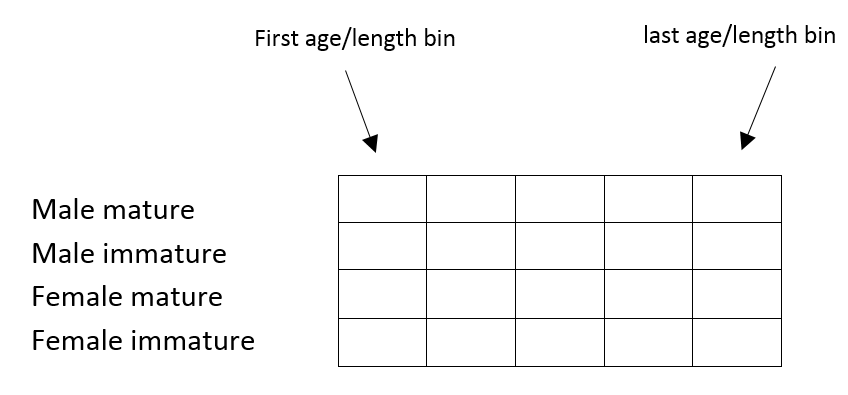
\includegraphics[scale=0.3]{Figures/partition.png}
		\caption{A visual representation of a partition}\label{Fig:part}
\end{figure}

So they define four time steps, labelled 1 through 4. Step 1 includes the non-spawning fishery. Step 2 includes the migration to the spawning area. Step 3 includes the spawning fishery. Step 4 includes recruitment and the migration back to the non-spawning area. (In fact, they could have used only 3 time steps, by using a single step in place of their steps 2 and 3. Because the default order of processes within a time step places migrations before fisheries, the processes would still have occurred in the right order.) There are other details to be sorted out, such as the proportion of natural mortality occurring in each time step and where observations occur, but this gives the basic idea.

This structure can be used to implement complex models, with intermingling of separate species and stocks, with complex migration patterns over multiple areas, and multiple sources of anthropogenic impact using different methods and covering different areas and times. However, we note that there is little point in using a complex structure to model a population when there are no observations to support that structure. In other words, use a structure for your model that is compatible with the data available. For information on how to define categories and using \CNAME's shorthand syntax see Section~\ref{sec:ShorthandSyntax-section}.

The model is run from an initial year up to the final(current) year. It can also be run past the final year to make projections --- things that happen in the future --- up to the final projection year.

An example, to specify a model with 2 categories (male and female) with ages 1-20 (with the last age a plus group) and an age-length relationship defined with the label \texttt{male\_growth} and \texttt{female\_growth}, then the \texttt{@model} example from above becomes,
{\small{\begin{verbatim}
		@model
		start_year
		final_year
		min_age 1
		max_age 20
		age_plus_group True
		initialisation_phases iphase
		time_steps step1 step2
\end{verbatim}}}

\subsection{\I{The state object and the partition}}

The key component of the state object is the partition, a matrix that store numbers of individuals at age for each category. A category represents a group of individuals that have the same specific attributes, examples of such attributes include life histories and growth rates, etc. For example, categories may include labels such as:

\begin{itemize}
\item Sex (male or female);
\item Area (any number of areas, named by the user);
\item Maturity (immature or mature);
\item Growth-path (any number of growth-paths);
\item Tag (any number of tagging events);
\item Species
\end{itemize}

A stock can be thought of as a population of individuals which recruits separately. See Section \ref{sec:maturity-notinpartition} for the treatment of maturity when it is not a category in the partition. 

So, you need to tell \CNAME\ the following: 

\begin{itemize}
\item	The minimum and maximum age classes in an age-based model.
\item	Whether there is an age-plus group.
\item The names of all categories.
\end{itemize}

Age classes are always one year wide, except that the maximum age group can optionally be a plus group. Users need to choose the minimum and maximum age classes. 

\CNAME\ allows categories of the partition to exist for certain years of the model. This is added for computational efficiency, when models contain a large number of categories that do not persist for all model years. Situations where this is beneficial is when a model contains a process that does a one off transition of fish from one category into another category in a subset of the model initialisation phases or years (for example, tagging events). Excluding categories for certain years can save a considerable amount of time as CASAL2 does not need to, for example, initialising empty categories or implement processes in time periods when they have no effect. 

Another important component of the state object in \CNAME\ are derived quantities. This includes quantities such as a mature biomass (for example, in fisheries models, the mid-spawning season biomasses of spawning fish, SSB) for either one or sum of more than one category. \CNAME\ derives through the command \command{derived\_quantity}, and may be required in the specification of some processes (i.e., in fisheries models, a recruitment process that  specifies a stock recruitment relationship requires the definition of a derived quantity that specifies the mid-season spawning stock biomass).

\subsection{\I{Time sequences}}

The time sequence of the model is defined in the following parts;
\begin{itemize}
  \item \I{Annual cycle}
  \item \I{Initialisation}
  \item \I{Model run years}
  \item \I{Projection year}s
\end{itemize}

\subsubsection*{\I{Annual cycle}}

The annual cycle is implemented as a set of processes that occur, in a user-defined order, within each year. Time-steps are used to break the annual cycle into separate components, and allow observations to be associated with different time periods and processes. Any number of processes can occur within each time-step, in any order (although there are limitations around mortality based processes - see Section~\ref{sec:mortality_block}) and can occur multiple times within each time-step. Note that time-steps are not implemented during the initialisation phases (effectively, there is only one time-step), and that the annual cycle in the initialisation phases can, optionally, be different from that which is applied during the model years.

\subsubsection*{\I{Mortality blocks}}\label{sec:mortality_block}

For every time step in an annual cycle there is an associated \emph{mortality block}. Mortality blocks are a key concept in \CNAME.

Mortality blocks are used to define the `point' in the model time sequence when observations (see Section~\ref{sec:observation-section}) are evaluated, and derived quantities (see Section~\ref{sec:derived-quantities}) are calculated.

A mortality block is defined as a consecutive sequence of mortality processes within a time step. The processes that are mortality processes are all pre-defined in \CNAME, and cannot be modified. These include all the processes described in subsection~\ref{sec:mortality}. 

\CNAME\ requires that each time step has exactly one mortality block. The achieve this, either all the mortality processes in a time step must be sequential (i.e., there can not be a non-mortality process between any two mortality processes within any one time step); or if no mortality processes occur in a time step then the mortality block is defined to occur at the end of the time step. 

\CNAME\ will error out if more than one mortality block occurs in a single time step. 

\begin{figure}[H]
	\centering
	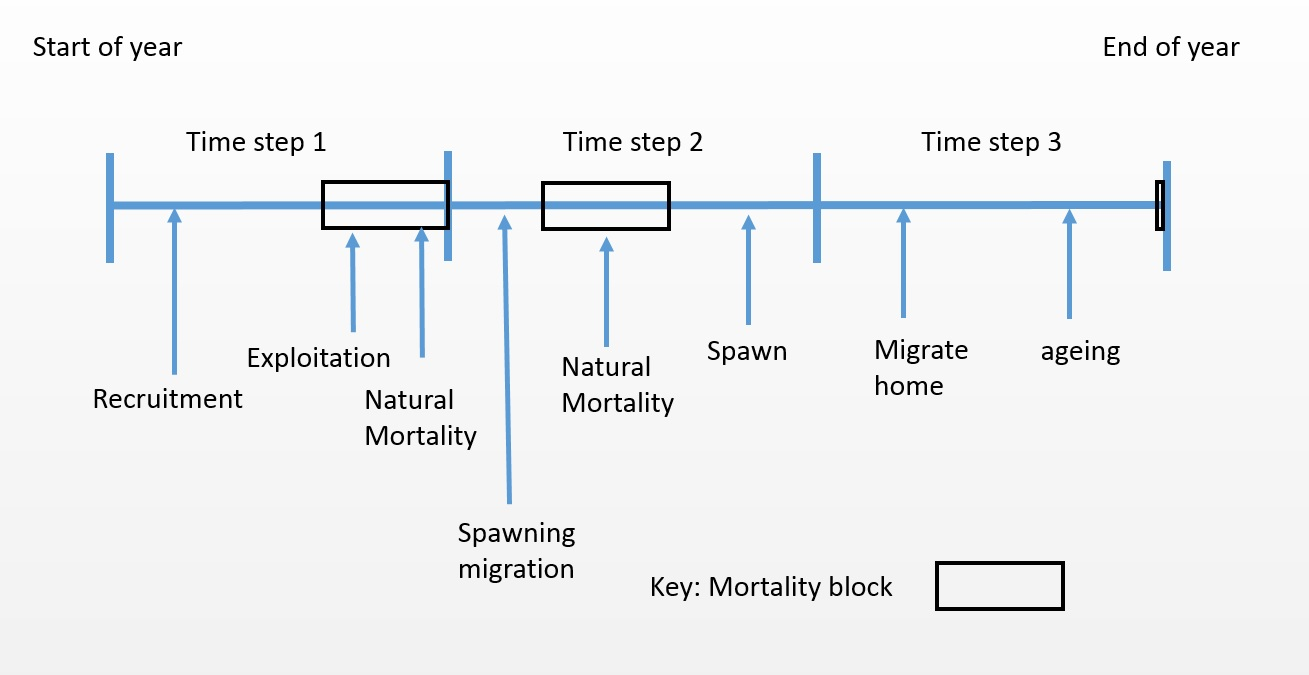
\includegraphics[scale=0.5]{Figures/annual_cycle.jpg}
	\caption{A visual representation of a hypothetical sequence for an annual cycle.}\label{Fig:annual}
\end{figure}

\subsubsection{\I{Initialisation}}\label{subsec:initialisation}

Initialisation is the process of determining the model starting state, whether it be equilibrium/steady state or some other initial state for the model (e.g exploited), prior to the start year of the model. This can be computationally expensive if a plus group is present in the partition.

There are multiple methods to initialise a partition in \CNAME. These methods are: iterative, fixed, derived, and Cinitial. 

Model initialisation can also occur in several phases\index{Initialisation!phases}, each of which can be a different method. These are carried out in sequence. At the end of all of the initialisations, \CNAME\ then runs the model years carrying out processes in each time step in the annual cycle.

The multi-phased initialisation allows the user to choose a number of initialisations that may assist with optimising the models for speed, initialise a non-equilibrium starting state, or resolve simple processes before introducing more complex ones.

Each phase of the initialisation defaults to have the same processes and in the same order as defined in the annual cycle. Although they can involve any number of processes using the \texttt{insert\_processes} subcommand.

In each initialisation phase, the processes defined for that phase are carried out and used as the starting point for the following phase or, if it is the last phase, then the years that the model is run over. 

Note that the \emph{first} initialisation phase is always initialised with each element (i.e., each age and category) set at zero. Note that you may need to be careful when using complex category inter-relationships or density dependent processes that depend on a previously calculated state, as they may fail when used in the first phase of an initialisation. 

Multi-phase iterations\index{Multi-phase iteration} can also be used to determine if the initialisation has converged. Here, add a second initialisation phase for, say, $1$ year (with the same processes applied). Then report the state at the end of the first and second phase. If these states are identical, then its likely that the initialisation has converged to an equilibrium state.

Syntax for including or excluding processes through the \texttt{insert\_processes} and  \texttt{exclude\_processes}. For the \texttt{insert\_processes} the syntax is;
{\small{\begin{verbatim}
		insert_processes time_step_label(process_label_in_annual_cycle) = label_new_process
\end{verbatim}}}
		An example of this is would be in the \command{time\_step} labelled \texttt{Oct\_Nov} include the \command{process} labelled \texttt{predationIni} before the \command{process} labelled \texttt{Instantaneous\_Mortality}
{\small{\begin{verbatim}
		insert_processes Oct_Nov(Instantaneous_Mortality)=predationIni
\end{verbatim}}}

if you want to include a process at the end of the time step you can use the following syntax,
{\small{\begin{verbatim}
		insert_processes Oct_Nov()=predationIni
		\end{verbatim}}}
To exclude a process from an initialisation phase the syntax is much simpler and can be done by the following subcommand in your \command{initialisation\_phase};

{\small{\begin{verbatim}
		exclude_processes process_label_in_annual_cycle
    	exclude_processes Instantaneous_Mortality	
		\end{verbatim}}}

The command above will remove the process \texttt{Instantaneous\_Mortality} during that particular initialisation phase.

\paragraph*{\I{Iterative Initialisation}}

The iterative initialisation is a general solution for initialising the model. The iterative method can be slow to converge, depending on the nature of the problem being resolved, but will work on even complex structured models that may be difficult or impossible to implement using analytic approximations. 

The number of iterations in the iterative initialisation can effect the model output, and these should be chosen to be large enough to allow the population state to fully converge. We recommend that a period of about two generations to ensure convergence. \CNAME\ can be requested to report a number of convergence statistics that can assist the user determine the level of convergence.

In addition, the iterative initialisation phase can optionally be stopped early if some user defined convergence criteria is met. For list of supplied years in the initialisation phase, convergence is defined as met if the proportional absolute summed difference between the state in year $t-1$ and the state in year $t$ ($\widehat{\lambda}$) is less than a user defined $\lambda$ where, 
\begin{equation}
  \widehat{\lambda} = \frac{\sum\limits_{i} \sum\limits_{j} \left|\text{element}(i,j)_t - \text{element}(i,j)_{t-1} \right|}{\sum\limits_{i} \sum\limits_{j} \frac{}{}\text{element}(i,j)_t}
\end{equation}

Hence, for an iterative initialisation you need to define;
\begin{itemize}
  \item The initialisation phases.
  \item The number of years in each phase and the processes to apply in each (default is the annual cycle).
\end{itemize}

An example of the syntax to implement this would be,
{\small{\begin{verbatim}
@model
...
initialisation_phases Iterative_initialisation

@initialisation_phase Iterative_initialisation
type iterative
years 50
lambda 0.0001
convergence_years 20 40
\end{verbatim}}}

\paragraph*{\I{Derived Initialisation}}

\texttt{Derived} initialisation is an analytical solution that calculates the equilibrium age structure and the plus group using a geometric series solution. The benefit of this method is it can be solved in max\_age - min\_age +1 years, so is computationally faster than the iterative initialisation phase. Users should be warned that we have found under some process combinations (for example. one way migrations) that this solution does not reach the exact equilibrium partition. We note that if using this method, that users confirm the partition has reached an equilibrium state by either comparing with and iterative initialisation, or by adding a second iterative initialisation phase of a limited number of iterations to confirm convergence.

An example of the syntax to implement this would be,
{\small{\begin{verbatim}
		@model
		...
		initialisation_phases Equilibrium_initialisation
		
		@initialisation_phase Equilibrium_initialisation
		type derived
		\end{verbatim}}}
	
\paragraph*{\I{Cinitial Initialisation}}

This initialisation is only available as a second or greater phase initialisation, and can only be applied after derived or iterative initialisation phases. The Cinitial factors that can be estimated to shift the initial population away from an equilibrium state prior to start year. If there is known exploitation before data exists for a population this can be a solution for estimating a non equilibrium population. Note that it may be advisable to include an observation of age composition data for the first year of the model in order to estimate the non equilibrium population state. 

An example of the syntax to implement this would be,

{\small{\begin{verbatim}
		@model
		...
		initialisation_phases Cinitial
		
		@initialisation_phase Cinitial
		type cinitial
		categories spawn.male+nonspawn.male 	spawn.female+nonspawn.female
		table n
		spawn.male+nonspawn.male   5e7 5e7 7e6 6e6 5e6 4e6 3e6 2e6 1e6 1e6 1e1 1e1 1e1 1e1	
		spawn.female+nonspawn.female 5e7 5e7 7e6 6e6 5e6 4e6 3e6 2e6 1e6 1e6 1e1 1e1 1e1 1e1
		end_table
		\end{verbatim}}}
	
		The cinitial factors can also be estimated using the following syntax
		
{\small{\begin{verbatim}	
	@estimate cinit_male
	parameter initialisation_phase[Cinitial].spawn.male+nonspawn.male
	same initialisation_phase[Cinitial].spawn.female+nonspawn.female
	lower_bound  2e2  2e2  2e2  2e2  2e2  2e2  2e2  2e2  2e2  2e2  2e0  2e0  2e0  2e0
	upper_bound  2e9  2e9  2e9  2e9  2e9  2e9  2e9  2e9  2e9  2e9  2e9  2e9  2e9  2e9
	type uniform
	\end{verbatim}}}

\paragraph*{\I{Fixed Initialisation}}

This is a user defined table that is taken to be the initial partition prior to the start year. Users have the ability to initialise models by specify the numbers at age for each category. Be careful when initialising models with this type, if the model applies processes that require derived quantities to be calculated in the initialisation phase. As this may cause undefined behaviour.

An example of the syntax to implement this would be,
{\small{\begin{verbatim}
		@model
		...
		initialisation_phases Fixed
		
		@initialisation_phase Fixed
		type state_category_by_age
		categories male female
		min_age 3
		max_age 10
		table n
		male   1000 900 800 700 600 500 400 700
		female 1000 900 800 700 600 500 400 700
		end_table
		\end{verbatim}}}

\subsection{\I{Model run years}}

Following initialisation, the model then runs over a number of user-defined years from (initial\_year to final\_year). For this part of the model, the annual cycle can be broken into separate time-steps, and observations can be associated with the state of the model at the end of any time-step, i.e., likelihoods for particular observations are evaluated, if required, within each time-step. 

Processes are carried out in the order specified within each time-step. These can be the same or different to the processes in initialisation phases of the model. 

The run years define the years over which the model is to run and the annual cycle within each year. The model runs from the start of year \argument{initial} and runs to the end of year \argument{current}. The projection part then extends the run time up to the end of year \argument{final}. 
\begin{itemize}
  \item The time-steps and the processes applied in each
  \item The initial year (i.e., the model start year)
  \item The final year (i.e., the model end year)
  \item The projection final year (i.e., the model projection end year)
\end{itemize}

\subsection{\I{Projection years}}\label{sec:projection}

Projecting is the process of running the model forwards into the future, using stochastic and or deterministic values for population dynamic parameters, such as recruitments and catches. Users invoke \CNAME\ to run in projection mode using the following command \texttt{casal2 -f 1}. The number the follows the \texttt{-f} parameter indicates how many projections you would like to undertake for each set of parameters supplied. This allows you to explore many future scenarios for a single set of parameters, this value should only be greater than 1 if you are applying a projection type that is stochastic. When running projections after a bayesian analysis you should add the \texttt{--tabular} parameter into the command. This will output a tabular report (see Section~\ref{sub:tabular}) which is easier to manipulate and run diagnostics on in the \R\ environment.

Projection years occur immediately after the model run years and defined as the \subcommand{final\_year + 1} upto and including \subcommand{final\_projection\_year}.

For a projection run in \CNAME\, a model is initialised and run through the model years from \argument{initial} to the \argument{final}. During this phase \CNAME\ stores all parameter values so that projection classes can (if the users choices) allow parameters before \subcommand{final\_year} to be projected (See end of this paragraph for an example of when you may want to do this). The model then is re-run from \argument{initial} to \argument{projection\_final\_year}, where any parameter can be either fixed or, if specified, drawn from a stochastic distribution or process during that time period. An example of when users may want to begin projecting a parameter before the projection phase has started is for year class parameters. Usually the last few year class parameters are poorly estimated (if they are estimated at all), although this depends on the quality and coverage of the compositional data that would inform these parameter or the precenese of a recruitment index. So users may wish to assume they are unknown and apply projection methods as they do for future values.

\CNAME\ does not have any default projections for when parameters are specified by year. These must be specified using the \command{project} command blocks. This is important for parameters that may vary from year to year (such as year class strength parameters), \CNAME\ should error out if users run \CNAME\ in projection mode but have not specified a \command{prject} block for the \subcommand{ycs\_values} parameter.

\CNAME\ allows any estimable parameter to be specified in a \command{project} block and then used in a projection. The available projection types for these parameters include constant, lognormal, empirical-lognormal, empirical re-sampling, or user-defined. To see all the projection classes available and examples of their syntax see Section~\ref{sec:projections}.

The subcommand that is common to all projection methods is the \subcommand{years},\subcommand{parameter} and \argument{multiplier} command. This is as it suggests a constant that is multiplied to the projected value after it has been derived by its respective method.

A \textbf{note} to users for the specific year class parameter, The definition of year applies to the \argument{ycs\_years} not the model years. As defined in Section~\ref{subsubsec:BH-recruitment}, \argument{ycs\_years} are offset between time of spawning and when they enter the partition. 

\subsection{\I{Population processes}}
Population processes are those processes that change the model state. Processes produce changes in the model partition, by adding, removing or moving individuals between ages and/or categories. The population processes include recruitment\index{Recruitment}, ageing\index{Ageing},  mortality\index{Mortality} events (e.g., natural and anthropogenic) and category transition processes\index{Category transition} (i.e., processes that move individuals between categories while preserving their age structure). See Section~\ref{sec:population-section} for a complete list of available processes.

There are two types of processes, processes that occur across multiple time steps in the annual cycle e.g \subcommand{mortality\_constant\_rate} and \subcommand{mortality\_instantaneous}. There are also processes that only occur within the time step they are defined. Each of these processes are carried out in the user-defined prescribed order when initialising the model, and then for a user-defined order in each year in the annual cycle\index{Annual cycle}. 

\subsubsection{\I{Recruitment}}

Recruitment processes are defined as a process that introduces new individuals into the partition. \CNAME\ currently implements two types of recruitment process, constant recruitment\index{Recruitment ! Constant} and  \I{Beverton-Holt recruitment}\index{Recruitment ! Beverton-Holt} \citep{1203}.

In the recruitment processes, the number of individuals are added to a single age class within the partition, with the amount defined by the type of recruitment process and its function. If more than one category is defined, then the proportion of recruiting individuals to be added to each category is specified by the \argument{proportions} parameter, or multiple recruitment processes can be defined. For example, if recruiting to categories labelled male and female, then you might set the proportions as $0.5$ and $0.5$ respectively to denote that half of the recruits recruit to the male category and the remaining half to the female category. 

An important note here is that recruitment can differ from a spawning event or the creation of a cohort/year class. In a fisheries context recruitment usually refers to indivisuals 'recruiting' to the fishery. This is done for a few reasons, one being often we do not have a lot of information relating to age classes between spawning and data collection i.e. an information gap exists. Once again in a fisheries context this information gap can refer to the time between spawning and being vulnerable to a survey or fishery for data collection. Thus users may only want to model the population for which data is available. This offset between spawning and recruitment is parameratised either by the recruitment variable \texttt{age} or \texttt{min\_age} (the default value for the \texttt{age} parameter in the recruitment process). For CASAL users the parameter \texttt{age} is the same as \texttt{y\_enter} in CASAL.

For the constant and Beverton-Holt recruitment processes, the  number of individuals following recruitment in year $y$ is,  
\begin{equation}
N_{y,a,j} \leftarrow N_{y,a - 1,j} + p_j(R_{y,a})
\end{equation}
where $N_{y,a,j}$ is the numbers in category $j$ at age $a$, $p_j$ is the proportion to category $j$, and $R_{y,a}$ is the number of recruits for year $y$. See below for how $N_{y,a,j}$ is determined in each of these cases.

\subsubsection*{\I{Constant Recruitment}}

In the constant recruitment process the total number of recruits added each year $y$ in age $a$ is $R_{y,a}$, and is simply $p_j(R_0)$, i.e.
\begin{equation}
  R_{y,a,j} = p_j(R_0)
\end{equation}

Constant recruitment recruits a constant number of individuals each year. It is equivalent to a Beverton-Holt recruitment process with steepness set equal to one (i.e., $h=1$).

For example, to specify a constant recruitment process, where individuals are added to male and female immature categories at $age=1$ evenly (\texttt{proportions} = 0.5), and the number to add is $R_0=5 \times 10^5$, then the syntax is

{\small{\begin{verbatim}
	@process Recruitment
	type constant_recruitment
	categories male.immature female.immature
	proportions 0.5 0.5
	r0 500000
	age 1
\end{verbatim}}}

\subsubsection*{\I{Beverton-Holt recruitment}}\label{subsubsec:BH-recruitment}

In the Beverton-Holt recruitment process the total number of recruits added each year is $R_y$, and is the product of the average recruitment $R_0$, the annual year class strength multiplier, $YCS$, and the stock-recruit relationship i.e.,
\begin{equation}\label{eq:BH}
  R_{y,a,j} = p_j(R_0 \times YCS_{ycs\_year} \times SR(SSB_{ycs\_year}))
\end{equation}
where
\begin{equation}\label{eq:year_class}
ycs\_year = y - \texttt{ssb\_offset}
\end{equation}

where $a$ is the parameter \texttt{age}, $p_j$ is the proportion of recruits to enter category $j$ and \texttt{ssb\_offset} is the lag between spawning and recruitment. As stated earlier recruitment refers to the recruitment into the population and may differ from the spawning event. See two paragraphs below on more information about \texttt{ssb\_offset}, but in general this parameter shouldn't be specified by the user.

$SR$ is the Beverton-Holt stock-recruit relationship parametrised by the steepness $h$,
\begin{equation}\label{eq:BH_SR}
SR(SSB_y) = \frac{SSB_y}{B_0} / \left( 1-\frac{5h-1}{4h} \left( 1-\frac{SSB_y}{B_0} \right) \right)
\end{equation}

Note that the Beverton-Holt recruitment process requires a value for \Bzero\ and $SSB_y$ to resolve the stock-recruitment relationship. Here, a derived quantity (see Section \ref{sec:derived-quantities}) must be defined that provides the annual $SSB_y$ for the recruitment process. \Bzero\ is then defined as the value of the $SSB$ at the end of one of the initialisation phases, this initialisation phase is defined by the parameter \texttt{b0\_intialisation\_phase}. During initialisation the $YCS$ multipliers are assumed to be equal to one, and recruitment that happens in the initialisation phases that occur before and during the phase when \Bzero\ is determined is assumed to have steepness $h=1$ (i.e. in those initialisation phases, recruitment is simply equal to \Rzero). Recruitment in the initialisation phases after the phase where \Bzero\ was determined follow the Beverton-Holt stock-recruit relationship defined above. \Rzero\ and \Bzero\ have a direct relationship when there are no density dependent processes in the annual cycle, for this reason users can choose to initialise models using \Bzero\ or \Rzero.

\texttt{ssb\_offset} should not be manually given by the user in commonplace, \CNAME\ determines \texttt{ssb\_offset} by the order of ageing, recruitment, spawning and the recruitment parameter \texttt{age}, 
\begin{itemize}
	\item If recruitment then ageing then spawning, then \texttt{ssb\_offset} should equal \texttt{age} + 1.
	\item If spawning then ageing then recruitment, then \texttt{ssb\_offset} should equal \texttt{age} - 1.
	\item else \texttt{ssb\_offset} = \texttt{age}
\end{itemize}

The certain scenarios where the user will manually want to input these values is if there are multiple ageing processes in the annual cycle. We have not coded \CNAME\ to deal with this situation so will be up to the user to define the \texttt{ssb\_offset}.

Another important input parameter is the \texttt{ycs\_years} which is defined in Equation~\eqref{eq:year_class}. When referencing the parameter \texttt{ycs\_values} you should always reference it by the \texttt{ycs\_years} parameter, this is important to note for when defining \command{estimate}, \command{project} and \command{time\_varying} blocks for the parameter \texttt{ycs\_values}. An example follows

Year classes values are standardised using the Haist parametrisation suggested by V. Haist. Here, the model parameter \texttt{ycs\_values} is a vector \textbf{Y}, covering years from \texttt{start\_year} - \texttt{ssb\_offset} to \texttt{final\_year} - \texttt{ssb\_offset}, as defined by the parameter \texttt{ycs\_years}. The year class strengths are calculated by $YCS_i=Y_i/\bar{\textbf{Y}}$ where the mean is calculated over the user-specified years \texttt{standardise\_ycs\_years}. Then,
\[
YCS_i = 
\begin{cases}
Y_i / mean_{y \in S}(Y_y) & :y \in S\\
Y_i					 & :y \notin S
\end{cases}
\]

where S is the set of years from \texttt{standardise\_ycs\_years}. One effect of this parametrisation is that\Rzero\ is then defined as the mean estimated recruitment over the years S, because the mean year class multiplier over these years will always be one.

Typically, the user will define \texttt{standardise\_ycs\_years} to span the years for which they expect to have reasonable estimates of YCSs. Often, the user will wish to force $Y_y=1$ for some or all years $y\in S$ (this is equivalent to forcing Ry=R0 x SR) by setting the lower and upper bounds of these Ys to be 1. An exception to this might occur for the most recent YCSs, which the user may want to estimate, but not include in the definition of R0 (because the estimates are based on too few data). Note that, optionally, the user may exclude one or more years from within the range from the averaging process of the Haist parameterisation. 

The advantage of the Haist parameterisation is that the user need no longer use a large penalty to force the mean of the YCS parameter to be 1 (though they should still use a small penalty to stop the mean of Y from drifting). This may improve MCMC performance.  projected YCS are not affected by this feature. A disadvantage with this parameterisation in a Bayesian analysis is that the prior refers to the Y’s, not the YCS.

An example of a the configuration of the Beverton-Holt recruitment process, where individuals are added to the category `immature' at $age=1$, and the number to add is $R_0=5 \times 10^5$. \texttt{SSB\_derived\_quantity} is a derived quantity that specifies the total spawning stock biomass that contributed to the this year class, with \Bzero\ the value of the derived quantity at the end of the initialisation phase labelled \texttt{phase1}. The $YCS$ are standardised to have mean one in the period 1995 to 2004, and recruits enter into the model two years following spawning.


{\small{\begin{verbatim}
	@process Recruitment
	type recruitment_beverton_holt
	categories immature
	proportions 1.0
	r0 500000
	b0_initialisation_phase phase1
	steepness 0.75
	age 1
	ssb SSB_derived_quantity
	standardise_ycs_years 1995:2004
	ycs_years 1994 1995 1996 1997 1998 1999 2000 2001 2002 2003 2004 2005 2006
	ycs_values   0.65    0.87    1.6    1.13    1.0235    0.385   2.653    1.35    1    1    1    1    1
\end{verbatim}}}

So, to specify a Beverton-Holt recruitment for each stock, the following information is required:
\begin{enumerate}
	\item YCS, starting from year (\texttt{start\_year} - \texttt{ssb\_offset}) and extending up to year (\texttt{final\_year} - \texttt{ssb\_offset}).
	\item The value of \texttt{age} aka \texttt{y\_enter} to CASAL users.
	\item the steepness parameter \texttt{h}.
	\item In a multi category model, the proportion of recruits for each category.
	\item label for the derived quantity
\end{enumerate}

Defining a \command{recruitment} block with a \command{initialisation\_phase} (Section~\ref{subsec:initialisation}) type = \subcommand{derived}. Ususally in a recruitment processes you only need to define the categories that recieve recruits, for example if you had a model that had a spawning area different from the are that recruits enter the population at, you would want an area explicit model containing spawning categories and recruiting categories. You can just specify the recruited categories in the subcommand \subcommand{categories}. As these will be the categories recieving recruits. \textbf{If} you have \command{initialisation\_phase}, \subcommand{type=derived} you need to specify all categories that are apart of that recruitment process. using the following example this would be defined as;

{\small{\begin{verbatim}
		@process Recruitment
		type recruitment_beverton_holt
		categories recruits.male recruits.female spawn.male spawn.female
		proportions 0.5 0.5 0.0 0.0
		r0 500000
		ssb SSB
		....
		\end{verbatim}}}
note the proportions = 0.0, this is needed because of how the derived initalisation phase works, it finds a solution for when \subcommand{r0} = 1.0 based on a infinite geometric series for the plus group, and scales the initial partition by \subcommand{r0}. Thus if you did not include all categories not all categories would be initialised to true values and give possibly messed up answers. This is cauton and will come up again in fishery based models where you have multiple stocks then you need to list all the categories that make up the stock.
\subsubsection{\I{Ageing}\label{sec:ageing}}

The ageing process `ages' individuals --- it simply moves all individuals in the named categories $i$ to the next age class $j + 1$, or accumulates them if the last age class is a plus group. 

The ageing process is defined as,
\begin{equation}
  \text{element}(i,j) \leftarrow \text{element}(i,j-1)
\end{equation}

except that in the case of the plus group (if defined), 
\begin{equation}
  \text{element}(i,age_{\text{max}}) \leftarrow \text{element}(i,age_{\text{max}}) + \text{element}(i,age_{\text{max}-1}).
\end{equation}

For example, to apply ageing to the categories \texttt{immature} and \texttt{mature}, then the syntax is,

{\small{\begin{verbatim}
	@process Ageing
	type ageing
	categories immature mature
	\end{verbatim}}}

Note that ageing is \emph{not} applied by \CNAME\ by default. As with other processes, \CNAME\ will not apply a process unless its defined and specified as a process within the annual cycle. Hence, it is possible to specify a model where a category is not aged. \CNAME\ will not check or otherwise warn if there is a category defined where ageing is not applied.

\subsubsection{\I{Mortality}\label{sec:mortality}}

Six types of mortality processes are permissible in \CNAME, constant rate, event, biomass-event, Hollings mortality, initialisation mortality event and instantaneous. These processes remove individuals from the partition, either as a rate, as a total number (abundance), as a biomass of individuals or as a mixture of these. Note that \CNAME\ does not (yet) implement the Baranov catch equation but instantaneous mortality is an approximation to the baranov catch equation. To apply both natural and biomass-event mortality, users can use \texttt{mortality\_instantaneous}. Note that all mortality processes occur within a mortality block of a time step see Section~\ref{sec:mortality_block} for more information and definitions on mortality blocks. 

\paragraph{Constant mortality rate}

To specify a constant annual mortality rate \index{Constant mortality}($M=0.2$) for categories `male' and `female', then, 
{\small{\begin{verbatim}
@process NaturalMortality
type mortality_constant_rate
categories male female
selectivities One One
m 0.2 0.2
\end{verbatim}}}

\begin{equation}
D_{j,t} = \sum_a N_{a,j} (1 - \exp{S_{a,j} M_j p_t})
\end{equation}
Where, $D_{j,t}$ is the number of deaths in category $j$ in time step $t$, $N_{a,j}$ is the number of individuals in category $j$ at age $a$. $S_{a,j}$ is the selectivity value for age $a$ in category $j$, $M_j$ is the mortality rate for category $j$, and $p_t$ is the proportion of the mortality rate to apply in time step $t$.

Note that the mortality rate process requires a selectivity. To apply the same mortality rate over all age classes, use a selectivity defined as $S_j=1.0$ for all ages $j$, e.g.,

{\small{\begin{verbatim}
@selectivity One
type constant
c 1
\end{verbatim}}}

\paragraph{Event and biomass-event mortality}

The event mortality process\index{Event mortality} and biomass mortality\index{Biomass event mortality} processes act in a similar manner, except that they remove a specified abundance (number of individuals) or biomass respectively. These can be used to include anthropogenic mortality where numbers of removals are known, for example, fishing in a fisheries model, rather than applying mortality as a rate. 

In these cases, the abundance or biomass removed is also constrained by a maximum exploitation rate. \CNAME\ removes as many individuals or as much biomass as it can while not exceeding the maximum exploitation rate. When minimising, event mortality processes require a penalty to discourage parameter values that do not allow the defined number of individuals to be removed. Here, the model penalises those parameter estimates that result in an too low a number of individuals in the defined categories (after applying selectivities) to allow for removals at the maximum exploitation rate. See Section \ref{sec:penalties} for more information on how to specify penalties.

For example, the event mortality applied to user-defined categories $i$, with the numbers removed at age $j$ determined by a selectivity-at-age $S_j$ is applied as follows:

First, calculate the vulnerable abundance for each category $i$ in $1 \ldots I$ for ages $j = 1 \ldots J$ that are subject to event mortality,
\begin{equation}
  V(i,j) = S(j) N(i,j)
\end{equation}

And hence define the total vulnerable abundance $V_{total}$ as,
\begin{equation}
  V_{total}  = \sum\limits_i {\sum\limits_j {V(i,j)}} 
\end{equation}

Hence the exploitation rate\index{Maximum exploitation rate} to apply is 
\begin{equation}
U = \begin{cases}
  C/V_{total}, & \text{if $C/V_{total} \leq U_{max}$} \\
  U_{max}, & \text{otherwise}\\ 
  \end{cases} 
\end{equation}

And the number removed $R$ from each age $j$ in category $i$ is,
\begin{equation}
  R(i,j) = UV(i,j)
\end{equation}

For example, to specify an \textbf{abundance based} fishing mortality process in a fisheries model, with catches given for a set of specific years, over categories `immature' and 'mature', with selectivity `FishingSel' and assuming a maximum possible exploitation rate of 0.7, then the syntax would be,

{\small{\begin{verbatim}
	@process Fishing
	type event_mortality
	categories immature mature
	years 2000 2001 2002 2003
	U_max 0.70
	selectivities FishingSel FishingSel
	penalty event_mortality_penalty
	\end{verbatim}}}

Another example of a \textbf{biomass} based fishing mortality process with the same characteristics as earlier.

{\small{\begin{verbatim}
		@process Fishing
		type mortality_event_biomass
		categories immature mature
		years 2000 2001 2002 2003
		U_max 0.70
		selectivities FishingSel FishingSel
		penalty event_mortality_penalty
		\end{verbatim}}}
\paragraph{Instantaneous mortality}

The instantaneous mortality process\index{Instantaneous mortality} is a process that combines both natural mortality and event biomass mortality into a single process. This allows the natural mortality to occur occurs across multiple time steps, and can specify multiple instances of event mortality to account for, say, multiple fisheries operating sequentially or concurrently. This process applies half the natural mortality in each time step, then the mortalities from all the concurrent fisheries instantaneously, then the remaining half of the natural mortality.

When instantaneous mortality is applied the following equations are used.

\begin{itemize}
	\item An exploitation rate (actually a proportion) is calculated for each fishery, as the catch over the selected-and-retained biomass,
	$$ U_f = \frac{C_f}{\sum_j \bar{w}_jS_{f,j}n_j e^{-0.5tM_j}}$$
	\item The fishing pressure associated with fishery $f$ is defined as the maximum proportion of fish taken from any element of the partition in the area affected by fishery $f$,
	$$ U_{f,obs} = max_j(\sum_k S_{k,j}U_k) $$
	where the maximum is over all partition elements affected by fishery $f$, and the summation is over all fisheries $k$ which affect the jth partition element in the same time step as fishery $f$.
	
In most cases the fishing pressure will be equal to the exploitation rate (i.e., $U_{f,obs} = U_f$), but they can be different if (a) there is another fishery operating in the same time step as fishery $f$ and affecting some of the same partition elements, and/or (b) the selectivity $S_{f,j}$ does not have a maximum value of 1.
	
There is a maximum fishing pressure limit of $U_{f,max}$ for each fishery $f$. So, no more than proportion $U_{f,max}$ can be taken from any element of the partition affected by fishery $f$ in that time step. Clearly $0 \leq U_{max} \leq 1$. It is an error if two fisheries which affect the same partition elements in the same time step do not have the same $U_max$.

For each $f$, if $U_{f,obs} > U_{f,max}$, then $U_f$ is multiplied by $U_{f,max}/U_{f,obs}$ and the fishing pressures are recalculated. In this case the catch actually taken from the population in the model will differ from the specified catch, $C_f$.
	
\item The partition is updated using
	$$ n'_j = n_j exp(-tM_j)\big[1 - \sum_f S_{f,j} U_f \big] $$ 
\end{itemize}

An example of the syntax is if we want to apply natural mortality of $0.20$ across three time steps on both male and female categories. And we have two method of removals (fisheries) \texttt{FishingWest FishingEast} with there respective catches known for years 1975:1977 in kilograms. These are given in the \texttt{catches} table and information on selectivities, penalties and maximum exploitation rates are given in the \texttt{fisheries} table.

{\small{\begin{verbatim}
	@process instant_mort
	type mortality_instantaneous
	m 0.20
	time_step_ratio 0.42 0.25 0.33
	selectivities One
	categories male female
	units kgs

	table catches
	year FishingWest FishingEast
	1975	80000	111000
	1976	152000	336000
	1977	74000	1214000
	end table

	table method
	method       category  selectivity u_max   time_step penalty
	FishingWest   stock     westFSel    0.7     step1     CatchPenalty
	FishingEast   stock     eastFSel    0.7     step1     CatchPenalty
	end_table
	\end{verbatim}}}

Referencing catch parameters for use in projecting, time\_varying and estimating uses the following syntax;
{\small{\begin{verbatim}
		parameter process[mortality_instantaneous].method_"method_label"{2018}
		\end{verbatim}}}
	where \subcommand{"method\_label"} is lower case from your \subcommand{catch} or \subcommand{method} table taking the following earlier example;

{\small{\begin{verbatim}
		parameter process[instant_mort].method_FishingWest{2018}
		\end{verbatim}}}
		
\paragraph{Hollings mortality rate}

The density-dependent Holling mortality process\index{Holling mortality} applies the Holling Type II and Type III functions \citep{Holling1959}, but is generalised using the Michaelis-Menten equation \citep{MentenMichaelis1913}. The function removes a number or biomass from a set of categories according to their total (selected) abundance (or biomass)and some 'predator' abundance (or biomass), but constrained by a maximum exploitation rate.

For example, the mortality applied to user-defined categories $k$, with the numbers removed at age $l$ determined by a selectivity-at-age $S(l)$ is applied as follows:

First, calculate the total predator abundance (or biomass) over all predator categories $k$ in $1 \ldots K$ and ages $l = 1 \ldots L$ that are applying the mortality,
\begin{equation}
	P(k,l) = S_{predator}(l) N_{predator}(k,l)
\end{equation}

And define the total predator abundance (or biomass) $P_{total}$ as,
\begin{equation}
	P_{total}  = \sum\limits_K {\sum\limits_L {P(k,l)}} 
\end{equation}

Then, calculate the total vulnerable abundance (or biomass) over all prey categories $k$ in $1 \ldots K$ and ages $l = 1 \ldots L$ that are subject to the mortality,
\begin{equation}
	V(k,l) = S_{prey}(l) N_{prey}(k,l)
\end{equation}

And hence define the total vulnerable abundance (or biomass) $V_{total}$ as,
\begin{equation}
	V_{total}  = \sum\limits_K {\sum\limits_L {V(k,l)}} 
\end{equation}

and then, the the number to remove is determined as,
\begin{equation}
	R_{total} = P_{total} \frac{a  V_{total}^{x-1}}{b + V_{total}^{x-1}}
\end{equation}
where $x=2$ for Holling type II function,  $x=3$ for Holling type III function, or any value of $x \geq 1$ for the generalised Michaelis-Menten function, and $a > 0$ and $b > 0$ are the Holling function parameters.

Hence the exploitation rate\index{Maximum exploitation rate} to apply is 
\begin{equation}
	U = \begin{cases}
		R_{total}/V_{total}, & \text{if $R_{total}/V_{total} \leq U_{max}$} \\
		U_{max}, & \text{otherwise}\\ 
	\end{cases} 
\end{equation}

And the number removed $R$ from each age $l$ in category $k$ is,
\begin{equation}
	R(k,l) = UV(k,l)
\end{equation}

The density-dependent Holling mortality process is applied either as a biomass or an abundance depending on the value of the \texttt{is\_abundance} switch.

For example, a biomass Holling type II mortality process on \texttt{prey} by our predator \texttt{predator} would have syntax,

{\small{\begin{verbatim}
		@process HollingMortality
		type Holling_mortality_rate
		is_abundance F
		a 0.08
		b 10000
		x 2
		categories prey
		selectivities One
		predator_categories predator
		predator_selectivities One
		u_max 0.8
		\end{verbatim}}}

\paragraph{Initialisation event or biomass-event mortality}

The Initialisation event mortality process\index{Initialisation event mortality} are specific processes that only can occur in the initialisation phase. It allows users to apply abundance or biomass mortality events specifically in initialisation phases. This can be useful if you wanted to deviate a model from equilibrium before model start. This process applies a single catch for all iterations within the initialisation phase, this process wont apply any mortality outside of the initialisation phase. It is advised that users use this process in conjunction with the \texttt{insert\_processes} command in the \command{initialisation\_phase} block, and not embed this process in the annual cycle. Example syntax to implement such a scenario,

{\small{\begin{verbatim}
initialisation_phases Equilibrium_state Predation_state
time_steps Oct_Nov Dec_Mar

@initialisation_phase Equilibrium_state 
type derived

@initialisation_phase Predation_state
type iterative
insert_processes Oct_Nov()=predation_Initialisation

@process predation_Initialisation
type initialisation_mortality_event
categories male.HOKI female.HOKI
catch 90000
selectivities Hakesl Hakesl

time_step Oct_Nov
processes Mg1 Instantaneous_Mortality

@time_step Dec_Mar 
processes Recruitment Instantaneous_Mortality
\end{verbatim}}}

Note how we have added the \texttt{initialisation\_mortality\_event} into the initialisation phase \texttt{Predation\_state} but not in the annual cycle. This was a case where the functionality has been applied.



\subsubsection{\I{Transition By Category}}

This process covers moves individuals between categories. Because the \CNAME\ partition user defined, this type of process is used to move individuals between categorised, and is used to specify processes such as maturation (move individuals from an immature to mature state) or migration (move individuals from one area to another). 

\paragraph{Annual transition by category}

A special case is annual transition by category, which allows a transition to occur in a specific subset of years only, where each year can have a different rate.

In both cases, there has to be a one to one relationship between the `from' category and the `to' category --- for every source category there is one target category. If however, you want to merge categories, then just repeat the `to' category multiple times. 

\begin{equation}
	N_{a,j} = N_{a,i} \times P_i \times S_{a,i}
\end{equation}
where $N_{a,j}$ is the number of individuals that have moved to category $j$ from category $i$ in age $a$ and $N_{a,i}$ is the number of individuals in category $i$. $P_i$ is the proportion parameter for category $i$ and $S_{a,i}$ is the selectivity at age $a$ for category $i$.

An example, to specify a simple spawning migration of mature males from a western area migrating to an eastern (spawning) area, then the syntax is
{\small{\begin{verbatim}
		@process Spawning_migration
		type transition_category
		from West.males	
		to East.males	
		selectivities MatureSel
		proportions 1
		\end{verbatim}}}

Where \texttt{MatureSel} is a selectivity that describes the proportion of age or length classes that are mature and thus move to the eastern area.

\subsubsection{\I{Tag Release events}}\label{sub:tag_release}

Tagging processes can be age or length based processes, where by numbers of fished are moved from an untagged category to a tagged category that the user has defined in the \command{Categories} block. Tag release processes can also account for tag induced mortality on individuals. Age based tag release events take a known number of individuals tagged for each age and do a straightforward category transition along with extra mortality. Length based tag release processes are more complicated, as \CNAME\ needs to calculate the age length matrix and exploitation by each length to then move the correct numbers at age based on the known lengths of release. \CNAME\ also allows for initial tag loss. An example of tag release by length process is as follows. 

{\small{\begin{verbatim}
		@process 2005Tags_shelf
		type tag_by_length 
		years 2005
		from male.untagged  female.untagged
		to male.2005  female.2005	
		selectivities MatureSel
		proportions 1
		selectivities ShelfselMale ShelfselFemale
		penalty tagging_penalty
		maximum_length 230
		plus_group False
		initial_mortality 0.1
		table proportions
		year 30 40 50 60 70 80 90 100 110 120 130 140 150 160 170 180 190 200 210 220
		2005  0 0 0.0580 0.1546 0.3380 0.1981 0.1643 0.0531 0.0242 0.0097 0 0 0 0 0 0 0 0 0 0
		end_table
		n 207
		U_max 0.999
		\end{verbatim}}}

The above process will move 207 individuals from a combination of male.untagged and female.untagged, based on the combination of growth rates and selectivity between the sexes.

\subsubsection{\I{Tag Loss}}

Tag Loss is the process where tags are lost from tagged categories over time from tag failure or getting knocked off. This process is applied as a instantaneous migration rate that can happen over multiple time steps in the annual cycle. This method assumes when tags are lost that the fish are transferred from the \subcommand{from} category to the \subcommand{to} category. How the tag loss rate is applied depends on whether the fish were only tagged with a single tag (\subcommand{tag\_number\_per\_animal = 1}), double tagged (\subcommand{tag\_number\_per\_animal = 2}) or $n$ tagged (\subcommand{tag\_number\_per\_animal = n}). The relationship is as follows

{\small{\begin{verbatim}
	@process Tag_loss
	type tag_loss
	categories tagged_fish
	tag_loss_rate 0.02
	time_step_ratio 0.25 0.75
	selectivities One
	tag_loss_type single
	year 1985
		\end{verbatim}}}

\subsection{\I{Derived quantities}\label{sec:derived-quantities}}

Some processes require, as arguments, a population value derived from the population state. These are termed \texttt{derived quantities}. Derived quantities are values, calculated by \CNAME\ at the end of a specified time-step in every year, and hence they have a single value for each year of the model. Derived quantities can be calculated as either an abundance or as a biomass. Abundance derived quantities are simply the count or sum of categories (after applying a selectivity). Biomass derived quantities are similar, except they are a measure of biomass. Derived quantities are also calculated during the initialisation phases, and hence the time-step during each phase must also be specified. If the initialisation time-steps are not specified, \CNAME\ will calculate the derived quantity during the initialisation phases in every year, at the end of the annual cycle. 

Derived quantities are required by some processes, for example the Beverton-Holt recruitment process. The Beverton-Holt recruitment process can require an equilibrium biomass ($B_0$) and annual spawning stock biomass values ($SSB_y$) to resolve the stock-recruit relationship. Here, these would be defined as the abundance or biomass of a part of the population at some point in the annual cycle for selected ages and categories, and would be calculated as a derived quantity.

Derived quantities are associated with a mortality block see section~\ref{sec:mortality_block} for more detail on mortality blocks. Users can ask for derived quantities partway through mortality blocks. Currently two methods are implemented in \CNAME\ to interpolate derived quantities part-way through a mortality block, these are \texttt{weighted\_sum} and \texttt{weighted\_product}, they are defined as,
\begin{itemize}
	\item \texttt{weighted\_sum}: after proportion $p$ of the mortality block, the partition elements are given by $n_{p,j} = (1 - p)n_j + p'_j$
	
	\item \texttt{weighted\_product}: after proportion $p$ of the mortality block, the partition elements are given by $n_{p,j} = n_j^{1-p} n'^p_j$
\end{itemize}
where, $n_p,j$ is the derived quantity at proportion $p$ of the mortality block for category $j$. $n_j$ is the quantity at the beginning of the mortality block and $n'_j$ is the quantity at the end of the mortality block.

As an example, to define a biomass derived quantity (say spawning stock biomass, SSB) for a model, evaluated at the end of the first time-step (labelled \texttt{step\_one}), over all 'mature' male and female categories and halfway through the mortality block using the \texttt{weighted\_sum} method, we would use the syntax,

{\small{\begin{verbatim}
@derived_quantity SSB
type biomass
time_step step_one
categories mature.male mature.female
selectivities One
time_step_proportion 0.5
time_step_proportion_method weighted_sum
\end{verbatim}}}

\subsection{\I{Age-length relationship}\label{sec:age-at-age}}

The age-length relationship defines the length at age (and the weight at length, see Section \ref{sec:mean-weight}) of individuals at age/category within the model. There are three length-age relationships available in \CNAME. The first is the naive no relationship (where each individual has length 1 irrespective of age). The second  and third are the von-Bertalanffy and Schnute relationships respectively. The length-at-age relationship is used to determine the length frequency, given age, and then with the length-weight relationship, a weight-at-age of individuals within an age/category. 

The three age-length relationships are,

\begin{description}
\item {None:} where the length of each individual is exactly 1 for all ages, in which case the \texttt{none} length-weight relationship must also be used.
\item{von Bertalanffy:}\index{von Bertalanffy growth curve} where length at age is defined as,
\begin{equation} 
\bar{s}(age)= L_\infty \left( 1 - \exp \left( -k \left(age-t_0 \right) \right) \right)
\end{equation}

\item{Schnute:}\index{Schnute growth curve} where length at age is defined as,
\begin{equation}
\bar{s}(age)=\displaystyle\begin{cases}
  \left[ y_1^b + (y_2^b - y_1^b) \dfrac{1-\exp \left(-a(age - \tau_1) \right)}{1-\exp \left(-a(\tau_2 - \tau_1) \right)} \right]^{1/b}, & \text{if $a\ne0$ and $b\ne0$} \\
  \AddVspace
  y_1 \exp \left[ \ln \left( y_2 / y_1 \right) \dfrac{1-\exp \left(-a(age - \tau_1) \right)}{1-\exp \left(-a(\tau_2 - \tau_1) \right)} \right], & \text{if $a\ne0$ and $b=0$} \\
  \AddVspace
  \left[ y_1^b + \left( y_2^b - y_1^b \right) \dfrac{age-\tau_1}{\tau_2 - \tau_1} \right]^{1/b}, & \text{if $a=0$ and $b\ne0$} \\
  \AddVspace
  y_1 \exp \left[ \ln \left( y_2/y_1 \right) \dfrac{age-\tau_1}{\tau_2 - \tau_1} \right] , & \text{if $a=0$ and $b=0$} \\
  \end{cases}
\end{equation}
\end{description}

The von Bertalanffy curve is parameterised by $L_\infty$, $k$, and $t_0$; the Schnute curve \citep{836} by $y_1$ and $y_2$, which are the mean lengths at reference ages $\tau_1$ and $\tau_2$, and $a$ and $b$ (when $b=1$, this reduces to the von Bertalanffy with $k=a$). 

When defining length-at-age in \CNAME, you must also define a length-weight relationship (see Section \ref{sec:mean-weight} below).

\subsubsection*{\I{Calculation of length-at-age (in an age-based model)}}

\subsubsection*{\I{Interpolation of length-at-age}}

\subsubsection*{\I{Length-weight relationship}\label{sec:mean-weight}}

There are two length-weight relationship,s available in \CNAME. The first is the naive no relationship. Here, the weight of an individual, regardless of length, is always 1. The second is the basic relationship. 

The two length-weight relationships are,

\begin{itemize}
  \item{None:} The length-weight relationship where  
  \begin{equation}
    \text{mean weight}=1
  \end{equation}
  \item{Basic:}\index{Basic length-weight relationship} The length-weight relationship where the mean weight $w$ of an individual of length $l$ is
  \begin{equation}
    w=a l^b
  \end{equation}
	Note that if a distribution of length-at-age is specified, then the mean weight is calculated over the distribution of lengths, and is
  \begin{equation}
	  w=(al^b)(1+cv^2)^{\frac{b(b-1)}{2}}
  \end{equation}
	where the $cv$ is the c.v. of lengths-at-age. This adjustment is exact for lognormal distributions, and a close approximation for normal distributions if the c.v. is not large \citep{1388}.
\end{itemize}

Be careful about the scale of $a$ --- this can easily be specified incorrectly. If the catch is in tonnes and the growth curve in centimetres, then $a$ should be on the right scale to convert a length in centimetres to a weight in tonnes. Note that there are reports available that can be used to help check that the units specified are plausible (see Section \ref{sec:report-section}).


\subsection{\I{Weightless model}\label{sec:weightless-model}}
If users would like to only model abundance and are not interested in converting the population to weight you can turn off the \command{length\_weight}, by specifing the keyword \subcommand{none} in the \command{age\_length} block. For example,
{\small{\begin{verbatim}
	@age_length age_size
	type schnute
	...
	length_weight none
	\end{verbatim}}}

If this specified in the model any biomass that is generated by \CNAME\ will actually be abundance, so be careful on intepretations when using this setting.

\subsection{\I{Maturity, in models without maturing in the partition}\label{sec:maturity-notinpartition}}

If maturity is not a character of the partition it can easily be derived at an instance in time using selectivities. Applying a maturity selectivity on to the partition allows \CNAME\ to use mature elements in processes, derive mature biomasses estimates (using derived quantities), and report the mature partition as an output.

\subsection{\I{Selectivities}\label{sec:selectivities}}
A selectivity is a function that can have a different value for each age class. Selectivities are used throughout \CNAME\ to interpret observations (Section \ref{sec:estimation-section}) or to modify the effects of processes on each age class (Section \ref{sec:population-section}). \CNAME\ implements a number of different parametric forms, including logistic, knife edge, and double normal selectivities. Selectivities are defined in there own command block (\command{selectivity}), where the unique label is used by observations or processes to identify which selectivity to apply.

Selectivities are indexed by age, with indices from \argument{min\_age} to \argument{max\_age}. For example, you might have an age-based selectivity that was logistic with $50\%$ selected at age $5$ and $95\%$ selected at age $7$. This would be defined by the \subcommand{type}=\argument{logistic} with parameters $a_{50}=5$ and $a_{to95}=(7-5)=2$. Then the value of the selectivity at age $x=7$ is $0.95$ and the selectivity at $x=3$ is $0.05$. Note selectivities can be length based, However Caution, more testing is needed for this functionality.

Note that the function values for some choices of parameters for some selectivities can result in an computer numeric overflow error (i.e., the number calculated from parameter values is either too large or too small to be represented in computer memory). \CNAME\ implements range checks on some parameters to test for a possible numeric overflow error before attempting to calculate function values. For example, the logistic selectivity is implemented such that if $(a50-x)/ato_95 > 5$ then the value of the selectivity at $x=0$, i.e., for $a50=5$, $ato_95=0.1$, then the value of the selectivity at $x=1$, without range checking would be $7.1 \times 10^{-52}$. With range checking, that value is $0$ (as $(a50 x)/ato_95=40 > 5$).

The available selectivities are;

\begin{itemize}
  \item Constant
  \item Knife-edge
  \item All values
  \item All values bounded
  \item Increasing
  \item Logistic
  \item Inverse logistic
  \item Logistic producing
  \item Double normal
  \item Double exponential
  \item Cubic spline (Not yet implemented)
\end{itemize}

The available selectivities are described below.

\subsubsection[Constant]{{constant}}

\begin{equation}
f(x)=C
\end{equation}

The constant selectivity has the estimable parameter C. 

\subsubsection[Knife-edge]{\argument{knife\_edge}}
\begin{equation}
f(x)= \begin{cases}
  0, & \text{if $x < E$} \\
  \alpha, & \text{if $x \ge E$}\\ 
  \end{cases} 
\end{equation}

The knife-edge ogive has the estimable parameter E and a scaling parameter $\alpha$, where the default value of $\alpha = 1$

\subsubsection[All-values]{\argument{all\_values}}\index{Selectivities!All-values}

\begin{equation}
f(x)=V_x
\end{equation}

The all-values selectivity has estimable parameters $V_{low}$, $V_{low+1}$ \ldots $V_{high}$. Here, you need to provide the selectivity value for each age class.

\subsubsection[All-values-bounded]{\argument{all\_values\_bounded}}\index{Selectivities!All-values-bounded}

\begin{equation}
f(x)=\begin{cases}
		 0, & \text{if $x < L$} \\
		 V_x, & \text{if $L \le x \le H$} \\
		 V_H, & \text{if $x > H$}
  \end{cases}
\end{equation}

The all-values-bounded selectivity has non-estimable parameters L and H. The estimable parameters are $V_L$, $V_{L+1}$ \ldots $V_H$. Here, you need to provide an selectivity value for each age class from $L \ldots H$.

\subsubsection[Increasing]{\argument{increasing}}\index{Selectivities!Increasing}

\begin{equation} 
f(x)=\begin{cases}
	  0, & \text{if $x < L$} \\
	  f(x-1)+ \pi_x(\alpha-f(x-1)), & \text{if $L \le x \le H$} \\
	  f(\alpha), & \text{if $x \ge H$} \\  
  \end{cases}
\end{equation}

The increasing ogive has non-estimable parameters $L$ and $H$. The estimable parameters are $\pi_L$, $\pi_{L+1}$ \ldots $\pi_H$ (but if these are estimated, they should always be constrained to be between 0 and 1). $\alpha$ is a scaling parameter, with default value of $\alpha = 1$. Note that the increasing ogive is similar to the all-values-bounded ogive, but is constrained to be non-decreasing.

\subsubsection[Logistic]{\argument{logistic}}\index{Selectivities!Logistic}

\begin{equation}
  f(x) = \alpha / [1+19^{(a_{50}-x)/a_{to95}}]
\end{equation}
 
The logistic selectivity has estimable parameters $a_{50}$ and $a_{to95}$. $\alpha$ is a scaling parameter, with default value of $\alpha = 1$. The logistic selectivity takes values $0.5 \alpha$ at $x=a_{50}$ and $0.95 \alpha$ at $x=a_{50}+a_{to95}$. 

\subsubsection[Inverse logistic]{\argument{inverse\_logistic}}\index{Selectivities!Inverse-logistic}

\begin{equation}
  f(x) = \alpha - \alpha / [1+19^{(a_{50}-x)/a_{to95}}]
\end{equation}
 
The inverse logistic selectivity has estimable parameters $a_{50}$ and $a_{to95}$. $\alpha$ is a scaling parameter, with default value of $\alpha = 1$. The logistic selectivity takes values $0.5 \alpha$ at $x=a_{50}$ and $0.95 \alpha$ at $x=a_{50}-a_{to95}$. 

\subsubsection[Logistic producing]{\argument{logistic\_producing}}\index{Selectivities!Logistic-producing}

\begin{equation} 
f(x)=\begin{cases}
	  0, & \text{if $x < L$} \\
	  \lambda(L), & \text{if $x=L$} \\
	  \left( \lambda(x)-\lambda(x-1) \right) / \left( 1-\lambda(x-1) \right), & \text{if $L < x < H$} \\
	  1, & \text{if $x \ge H$} \\  
  \end{cases}
\end{equation}

The logistic-producing selectivity has the non-estimable parameters $L$ and $H$, and has estimable parameters $a_{50}$ and $a_{to95}$. $\alpha$ is a scaling parameter, with default value of $\alpha = 1$. For category transitions, $f(x)$ represents the proportion moving, not the proportion that have moved. This selectivity was designed for use in an age-based model to model maturity. In such a model, a logistic-producing maturation selectivity will (in the absence of other influences) make the proportions mature follow a logistic curve with parameters $a_{50}$, $a_{to95}$.

\subsubsection[Double-normal]{\argument{double\_normal}}\index{Selectivities!Double-normal}

\begin{equation}
  f(x) = \begin{cases}
    \alpha 2^{-[(x- \mu)/\sigma_L ]^2}, & \text{if $x \leq \mu$} \\
    \alpha 2^{-[(x- \mu)/\sigma_R ]^2}, & \text{if $x \ge \mu$}\\
  \end{cases}
\end{equation} 

The double-normal selectivity has estimable parameters $a_1$, $s_L$, and $s_R$. $\alpha$ is a scaling parameter, with default value of $\alpha = 1$. It has values $\alpha$ at $x=a_1$, and $0.5 \alpha$ at $x=a_1-s_L$ and $x=a_1+s_R$. 

\subsubsection[Double-exponential]{\argument{double\_exponential}}\index{Selectivities!Double-exponential}

\begin{equation} 
f(x)=\begin{cases}
	  \alpha y_0(y_1 / y_0)^{(x-x_0)/(x_1-x_0)}, & \text{if $x \le x_0$} \\
	  \alpha y_0(y_2 / y_0)^{(x-x_0)/(x_2-x_0)}, & \text{if $x > x_0$} \\
  \end{cases}
\end{equation}

The double-exponential selectivity has non-estimable parameters $x_1$ and $x_2$, and estimable parameters $x_0$, $y_0$, $y_1$, and $y_2$.  $\alpha$ is a scaling parameter, with default value of $\alpha = 1$. It can be `U-shaped'. Bounds for $x_0$ must be such that $x_1 < x_0 < x_2$. With $\alpha=1$, the selectivity passes through the points $(x_1, y)$, $(x_0, y_0)$, and $(x_2, y_2)$. If both $y_1$ and $y_2$ are greater than $y_0$ the selectivity is `U-shaped' with minimum at $(x_0, y_0)$.

%\subsubsection[Spline]{\argument{spline}}\index{Selectivities!Spline}
%
%The spline selectivity implements a cubic spline that has non-estimable knots, and an estimable value for each knot. The cubic spline is either (i) a natural splines where the second derivatives are set to 0 at the boundaries, i.e., the values at the boundaries are horizontal, (ii) a spline with a fixed first derivative at the boundaries (linear, but not necessarily horizontal) and (iii) spline which turns into a parabola at the boundaries. 
%
\begin{figure}
	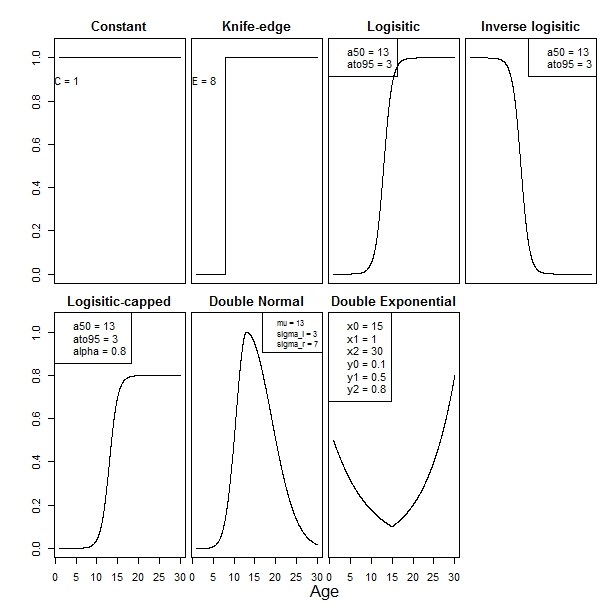
\includegraphics[scale = 0.7]{Figures/Selectivities.jpeg}
	\caption{Examples of the functional forms of selectivities available in \CNAME.}
\end{figure}

Selectivities \subcommand{all\_values} and \subcommand{all\_values\_bounded} can be addressed in additional priors using the following syntax,

{\small{\begin{verbatim}
		@selectivity maturity
		type all_values
		v 0.001 0.1 0.2 0.3 0.4 0.3 0.2 0.1
		
		## encourage ages 3-8 to be smooth.
		@additional_prior smooth_maturity
		type vector_smooth
		parameter selectivity[maturity].values{3:8}
		
		\end{verbatim}}}

\subsection{\I{Projections}\label{sec:projections}}
This section lists all the projections classes available, their functionality and an example of the syntax.
\paragraph*{\I{Constant}}
A parameter can either be fixed during all projection years or specified individually for each projection year. This is a deterministic assumption, where the parameter is assumed to be known without error during projection years.

{\small{\begin{verbatim}
		@project Future_ycs
		type constant
		parameter process[Recruitment].ycs_values
		years 2012:2016
		values 1 2 1 2 0.5
		multiplier 1
		\end{verbatim}}}
\paragraph*{\I{Empirical resampling}}

Parameters that have time components associated with them can be re-sampled uniformly with replacement over a range of years and used as the projected year values. The year range which users must specify are between \argument{start\_year} and \argument{final\_year}
{\small{\begin{verbatim}
		@project Future_ycs
		type empirical_sampling
		parameter process[Recruitment].ycs_values
		years 2012:2016
		start_year 1988
		final_year 2008
		multiplier 1
		\end{verbatim}}}


\paragraph*{\I{Lognormal}}
The parameters are originally drawn from a gaussian distribution in log space and exponentiated out to form the lognormal distribution,
\begin{equation}\label{eq:lognormal}
X_p = e^{\epsilon_p- 0.5\sigma^2}
\end{equation}
where $\epsilon_p\stackrel{iid}{\sim}N(\mu,\sigma)$ and $X_p$ is the projected value for parameter $X$, and $\mu$, $\sigma$ is the mean and standard deviation on the log scale. An example of applying this process is if we wanted to draw future year class parameters from a lognormal distribution with mean 1 and standard deviation 0.8, we would define the syntax as,

{\small{\begin{verbatim}
		@project Future_ycs
		type lognormal
		parameter process[Recruitment].ycs_values
		years 2012:2016
		mean 0
		sigma 0.8
		multiplier 1
		\end{verbatim}}}


\paragraph*{\I{Lognormal-Empirical}}
This class applies Lognormal draw as in the \argument{LogNormal} class but it allows the user to specify a year range which is re-sampled uniformly without replacement. These re sampled values are then used to calculate the standard deviation of the distribution. Then equation~\eqref{eq:lognormal} is used to generate future values with user defined $\mu$ and empirically calculated $\sigma$,

{\small{\begin{verbatim}
		@project Future_ycs
		type lognormal_empirical
		parameter process[Recruitment].ycs_values
		years 2012:2016
		mean 0
		start_year 1988
		final_year 2008
		multiplier 1
		\end{verbatim}}}

\paragraph*{\I{User Defined}}
This class allows users to use the equation parser to define the future values of a parameter during projection mode. This was originally set-up to apply harvest control rules (i.e. apply a management action, change in TACC based on the current or previos state). In fisheries this would be setting the catch based on an exploitation rate * vulnerable biomass, where the exploitation rate is based on some rule as shown in figure~\ref{fig:HCR}.

\begin{figure}[!h]\label{fig:HCR}
	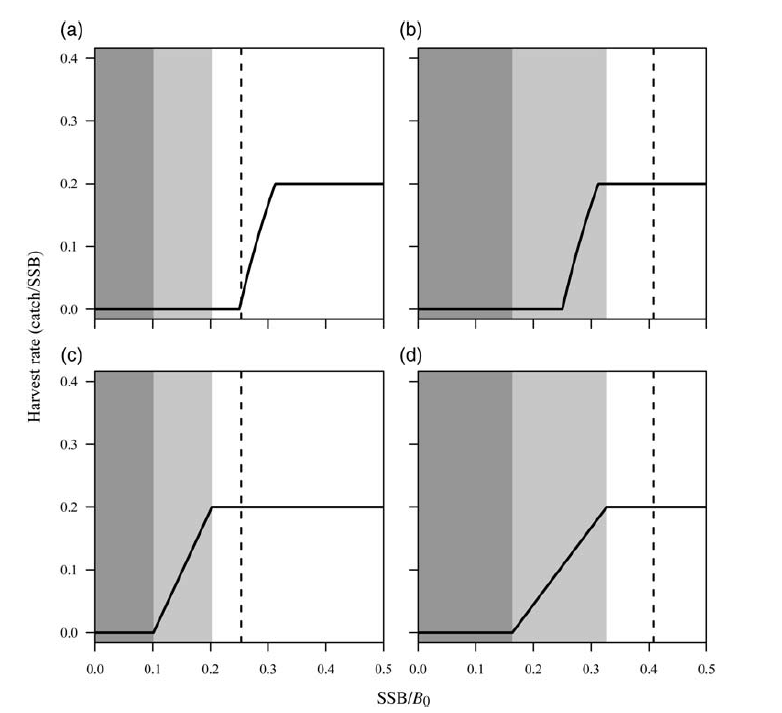
\includegraphics[scale=0.9]{Figures/HarvestControlRules.png}
	\caption{\textbf{Examples of control rules based on current stock status.}}
\end{figure}

\pagebreak
{\small{\begin{verbatim}
		@project HCR_2015
		type user_defined
		parameter process[Instantaneous_Mortality].method_Sub_Ant_F
		years 2015 
		equation if(derived_quantity[SSB].values{2014} / process[Recruitment].b0 <= 0.1, 0.0,
		if(derived_quantity[SSB].values{2014} / process[Recruitment].b0 > 0.1 && 
		derived_quantity[SSB].values{2014} / process[Recruitment].b0 < 0.2,
		derived_quantity[SSB].values{2014} * derived_quantity[SSB].values{2014}  
		/ process[Recruitment].b0,
		derived_quantity[SSB].values{2014} * 0.2))
		\end{verbatim}}}

The syntax of the equation parser is a bit difficult and care should be taken when writing it. In words the above equation is, if $\%B_{2014} \leq 0.1$ next years catch is 0.0, else if $\%B_{2014} > 0.1 \& \%B_{2014} \leq 0.2$, next years catch is equal to $\%B_{2014} * SSB_{2014}$, else set next years catch to $0.2 SSB_{2014}$

\subsection{\I{Time Varying Parameters}\label{sec:time_var}}

\CNAME\ has the functionality to vary any parameter annually between the start and final year of a model run. This can be for blocks of years or specific years if chosen. For years that are not specified the parameter will default to the input or if in a iterative state such as estimation mode, the value being trialled at that iteration. Method \texttt{type}'s for time varying a parameter are; \subcommand{constant}, \subcommand{random\_walk}, \subcommand{exogenous}, \subcommand{linear}, \subcommand{annual\_shift}, \subcommand{random\_draw}. This allows users to let a parameter be known in a year, be the result of a deterministic equation or stochastic. \textbf{Note} that we haven't implemented random effects so be careful on your intepretation if you choose to estimate parameters that control any stochastic time-varying method. This functionality was originally implemented for simulating more realistic observations. When you allow removals to have annual varying catchabilities, selectivities and other more realistic model components simulated observations become more real data and thus conclusions based on simulated data are more useful. The other driver was allowing mean or location parameters of selectivities to change between years based on an explanatory variable. An example of this is in the New Zealand Hoki fishery where we allow the $\mu$ and $a_{50}$ parameters to shift depending on when the fishing season. Discriptive analysis showed that when fishing was earlier relative to other years they caught smaller fish and vice versa. This can be shown in the Examples 2stock directory, implemented at line: 382 in population.csl2.

\subsubsection[Constant]{\argument{Constant}}\index{Time Varying Parameters!Constant}
Allows a parameter to have an alternative values during certain years, which can be estimated.
{\small{\begin{verbatim}
		@time_varying q_time_var
		type constant
		parameter catchability[survey_q].q
		years 1975:1988
		values 0.001
		\end{verbatim}}}

Users can also estimate these year values using the following syntax, a word of caution is that you shouldn't estimate the actual parameter and its time varying counterpart, as the time varying value will overwrite the actual parameter making the first value unidentifiable and an impossible optimization process.
{\small{\begin{verbatim}
		@estimate q_time_var
		type uniform
		parameter time_varying[q_time_var].values(1975:1976)
		lower_bound 1e-6 1e-6
		upper_bound 2 2
		\end{verbatim}}}

\subsubsection[Random Walk]{\argument{Random Walk}}\index{Time Varying Parameters!Random Walk}

A random deviate added into the last value drawn from a standard normal distribution. This has an estimable parameter $\sigma_p$ for each time varying parameter $p$. For reproducible modelling, it is highly recommended that users set the seed (see Section~\ref{sec:command-line-arguments}) when using stochastic functionality like this, otherwise reproducing models becomes almost impossible.
{\small{\begin{verbatim}
		@time_varying q_time_var
		type random_walk
		parameter catchability[survey_q].q
		distribution normal
		mean 0
		sigma 3
		\end{verbatim}}}

If the \texttt{parameter} specified in the \command{time\_varying} is associated with an \command{estimate} block then the parameter is constrained to stay within the lower and upper bounds of the \command{estimate} block. \textbf{WARNING}, if the parameter does not have an associated \command{estimate} block then there is no safe guard for a random deviate to put the parameter in a space where the model fails, i.e generates NA or INF values. to avoid this from happening it is recommended you specify an \command{estimate} block even though you are not estimating the parameter like below. A constraint whilst using this functionality is that a parameter cannot be less than 0.0, if it is \CNAME\ sets it equal to 0.01.

{\small{\begin{verbatim}
		@estimate survey_q_est
		type uniform
		parameter catchability[survey_q].q
		lower_bound 1e-6
		upper_bound 10
		\end{verbatim}}}
This will insure the random walk time varying process will set the any new candidate within the lower and upper bound of the \command{estimate} block.

\subsubsection[Annual shift]{\argument{Annual shift}}\index{Time Varying Parameters!Annual shift}
A parameter generated in year $y$ ($\theta'_y$) depends on the value specified by the user ($\theta_y$) along with three coefficients $a,b$ and $c$ as follows,

\begin{equation}
\bar{\theta}_y = \frac{\sum_{y}^Y\theta_y}{Y}
\end{equation}

\begin{equation}
\theta'_y = a \bar{\theta}_y + b\bar{\theta}_y^{2} + c\bar{\theta}_y^{3}
\end{equation}

\subsubsection[Exogenous]{\argument{Exogenous}}

Parameters are shifted based on an exogenous variable, an example of this is an exploitation selectivity parameters that may vary between years based on known changes in exploitation behaviour such as season, start time, and average depth of exploitation.
\begin{equation}
\delta_y = a(E_y - \bar{E})
\end{equation}

\begin{equation}
\theta'_y = \theta_y + \delta_y
\end{equation}
where $\delta_y$ is the shift or deviation in parameter $\theta_y$ in year $y$ to generate the new parameter value in year $y$ ($\theta'_y$). $a$ is an estimable shift parameter, $E$ is the exogenous variable and $E_y$ is the value of this variable in year $y$. For more information readers can see \cite{francis_03}.


\subsection{\I{Equation Parser}\label{sec:eq_parser}}
\CNAME\ has the ability to use an equation parser, this is currently implemented in two classes of the model, Projections (section~\ref{sec:projections}), Derived quantities (section~\ref{sec:derived-quantities}) and reports (section~\ref{sec:report-section}). Examples of syntax for implementing the equation parser follow from here. But for a more detailed look at the parser see \url{https://github.com/nickgammon/parser/blob/master/parser.cpp}\\


{\small{\begin{verbatim}
		equation process[Recruitment].r0 * (2-1)
		\end{verbatim}}}

Can apply routine mathematical functions such as \texttt{log}, \texttt{exp},\texttt{cos},\texttt{sin},\texttt{tan} such as;
{\small{\begin{verbatim}
		equation sqrt(process[Recruitment].r0)
		\end{verbatim}}}

Apply exponents,
{\small{\begin{verbatim}
		equation pow(2, 3)
		\end{verbatim}}}

evaluate the absolute of an equation using the \texttt{abs()} syntax,
{\small{\begin{verbatim}
		equation abs(sqrt(process[Recruitment].r0) * 1.33)
		\end{verbatim}}}
	
Use if else statements
{\small{\begin{verbatim}
		equation if(process[Recruitment].r0 > 23, 44, 55)
		## if R0 is greater than 23 return 44 else return 55
		\end{verbatim}}}
You can link if else statements as well but be warned the syntax becomes a bit messy, such as
{\small{\begin{verbatim}
		equation if(process[Recruitment].r0 > 23, 44, 
         		if(process[Recruitment].r0 > 10, 55, 66))
		## if R0 is greater than 23 return 44 else if R0 less than 23 but greater than 10 return 55, 
		else R0 must be less than 10 return 66
		\end{verbatim}}}

Constraints, are that you can only reference singletons so cannot apply an equation to vector parameters for example, you can't reference \subcommand{process[Recruit].ycs\_values\{1974:1980\}}. To see which parameters you can include in an equation parser go to the syntax section (Section~\ref{sec:syntax}) any subcommand that has a \textbf{Type} Estimable should in theory be addressed in an equation parser.

With the equation parser it is difficult to catch all user configuration errors. Such as we cannot check whether a parameter that exists in the system has been populated when the user requires it. For example if you wanted to say that next years (2015) removals was based on the this years (2014) state of the population. The user can easily specify the wrong year;
{\small{\begin{verbatim}
		parameter process[removals].catch
		year 2015
		equation derived_quantity[percent_b0].values{2020}
		\end{verbatim}}}
	
The above would be an acceptable equation but obviously will cause non-sensical results, because you are asking for a value in 2020 when you are in 2015. This is just a caution that although the equation parser is great and adds a great deal of flexibility, users should be careful because it is easy to mis-specify and near impossible for the development team to catch all errors.

\clearemptydoublepage{}
\section{\I{The estimation section}\label{sec:estimation-section}}

\subsection{\I{Role of the estimation section}\label{sec:role-of-the-estimation-section}}
The role of the estimation section is to define the tasks carried out by \CNAME: 

\begin{enumerate}
  \item Define the objective function (see Section \ref{sec:objective-function})
  \item Define the parameters to be estimated (see Section \ref{sec:estimate-free-parameters})
  \item Calculate a point estimate, i.e., the maximum posterior density estimate (MPD) (see Section \ref{sec:estimate-MPD})\index{Maximum posterior density estimate (MPD)}\index{MPD (Maximum posterior density estimate)}.
  \item Calculate a posterior profile selected parameters, i.e., find, for each of a series of values of a parameter, allowing the other estimated parameters to vary, the minimum value of the objective function (see Section \ref{sec:estimate-profiles}\index{Profiles}).
  \item Generate an MCMC\index{Monte Carlo Markov Chain (MCMC)} sample from the posterior distribution (see Section \ref{sec:estimate-MCMC}\index{MCMC}).
  \item Calculate the approximate covariance matrix of the parameters as the inverse of the minimizer\textquoteright{}s approximation to the \I{Hessian}, and the corresponding correlation matrix (see Section \ref{sec:estimate-MPD}\index{Covariance matrix}).
\end{enumerate}

The estimation section defines the objective function, parameters of the model, and the method of estimation (point estimates, Bayesian posteriors, profiles, etc.). The objective function is based on a goodness-of-fit measure of the model to observations, priors and penalties. See the observation section for a description of the observations, likelihoods, priors and penalties. 

\subsection{\I{The objective function}\label{sec:objective-function}}

In Bayesian estimation, the objective function is a negative log-posterior,

\begin{equation}\label{objective_function}
Objective(p)= - \sum\limits_i {\log \left[ {L\left( {{\bf{p}}|O_i } \right)} \right]}  - \log \left[ {\pi \left( {\bf{p}} \right)} \right]
\end{equation}

where $\pi$ is the joint prior density of the parameters $p$.

The contribution to the objective function from the likelihoods are defined in Section \ref{sec:likelihoods}. In addition to likelihoods, priors (see Section \ref{sec:priors}) and penalties (see Section \ref{sec:penalties}) are components of the objective function. Note that if the priors are specified as uniform, then the prior contribution is zero and the estimation problem turns into penalised-likelihood and not Bayesian.

Penalties can be used to ensure that the exploitation rate constraints on mortality events (i.e., fisheries) are not breached (otherwise there is nothing to prevent the model from having abundances so low that the recorded mortalities could not have been taken), penalties on category transitions (to ensure there are enough individuals to move), and possibly penalties to encourage estimated values to be similar or smooth, etc. Equation~\ref{objective_function} can mathematically reduce to a penalised likelihood equation if all priors are assumed to be uniform. This is because uniform priors have a zero contribution to the objective function so Equation~\ref{objective_function} reduces to likelihoods plus penalties.

\subsection{\I{Specifying the parameters to be estimated}\label{sec:estimate-free-parameters}}
The estimable parameters that will be estimated are defined using \command{estimate} commands (see Section \ref{sec:estimation-syntax}). An \command{estimate} command-block looks like\index{Estimating parameters},

{\small{\begin{verbatim}
  @estimate male.m
  parameter process[NaturalMortality].m{male}
  lower_bound 0.1
  upper_bound 0.4
  type uniform
\end{verbatim}}}

See Section \ref{sec:parameter-names} for instructions on how to generate the parameter name. At least one parameter is to be estimated if doing an estimation \texttt{-e}, profile \texttt{-p}, or MCMC \texttt{-m} run. Initial values for the parameters to be estimated will still need to be provided, and these are used as the starting values for the minimiser. However, these may be overwritten if you provide a set of alternative starting values (i.e., using  \texttt{\cname\ -i}, see Section \ref{sec:command-line-arguments}).

All parameters are estimated within bounds\index{Bounds}. For each parameter to be estimated, you need to specify the bounds and the prior\index{Priors} (\texttt{type}) (Section \ref{sec:priors}). Note that the bounds and prior for each parameter refer to the values of the parameters, not the actual values resulting from the application of the parameter to an equation. Bounds should be carefully chosen as they effect the space in which the minimisers search over. Some minimisers convert lower and upper bound into a minimisation space (for example -1,1 space for the numerical differences algorithm). If estimating only some elements of a vector, either define each element of the vector to be estimated (see \ref{sec:parameter-names}) or fix the others by setting the bounds equal.

\subsection{\I{Point estimation}\label{sec:estimate-MPD}}
Point estimation is invoked with \texttt{\cname\ -e}. Mathematically, it is an attempt to find a minimum of the objective function\index{Objective function}. \CNAME\ has multiple algorithms for solving (minimising) the optimisation problem. There are three non auto differential minimisers: numerical differences, differential evolution minimiser (\subcommand{de\_solver}), and the dlib minimiser. There are also three auto differential (AD) minimisers being: ADOL-C, CPPAD, and BETADIFF. For references see section \ref{sec:tech}. AD minimisers are recommended for complex models they are on average much faster and from my experience find a better minimum if exploring a complex objective surface. 

Recently with the number of parameters growing in these models, an important input parameter on most minimisers is the \subcommand{tolerance} parameter. This is the stopping rule that minimisers use to define when they have found a 'solution' (remember there is no guarantee that a solution is the global solution, such is the world we live in). Try  alternative starting values, this is easiliy done with the \texttt{-i parameter\_file.txt} in \CNAME. I digress, I highly recommend when estimating any model with \CNAME\ that you try smaller values for the \subcommand{tolerance} parameter. I have found for some models that if you make it say 0.00000002 that the solution is quite a bit different than when using the default (0.002). I believe this is not ideal behaviour from your model (Craig's Opinion) and that you should do some more investigative work on what parameters are causing the behaviour. An aside note: this will also effect your covariance matrix as with different tolerances and searchs you may end up with a different approximate hessian matrix which is inverted to solve for the covariance matrix. I thought that this might make a difference on MCMC results because the covariance is incorporated into the proposal distribution. However I have run a few MCMC's with varying tolerances and have found that doesn't effect the posterior distribution of the MCMC.
\subsubsection{\I{The numerical differences minimiser}}

The minimiser has three kinds of (non-error) exit status, depending on the minimiser: 

\begin{enumerate}
\item Successful convergence (suggests you have found a local minimum, at least).
\item Convergence failure (you have not reached a local minimum, though you may deem yourself to be `close enough' at your own risk).
\item Convergence unclear (the minimiser halted but was unable to determine if convergence occurred. You may be at a local minimum, although you should check by restarting the minimiser at the final values of the estimated parameters).
\end{enumerate}

You can choose the maximum number of quasi-Newton iterations\index{Quasi-Newton iterations} and objective function evaluations\index{Objective function evaluations} allotted to the minimiser. If it exceeds either limit, it exits with a convergence failure\index{Convergence failure}. We recommend large numbers of evaluations and iterations (at least the defaults of 300 and 1000) unless you successfully reach convergence with less. You can also specify an alternative starting point of the minimiser using \texttt{\cname\ -i}.

We want to stress that the minimisers are local optimisation algorithms trying to solve a global optimisation problem. What this means is that, even if you get a 'successful convergence'\index{Successful convergence} message, your solution may be only a local minimum\index{Local minimums}, not a global one. To diagnose this problem, try doing multiple runs from different starting points and comparing the results, or doing profiles of one or more key parameters and seeing if any of the profiled estimates finds a better optimum than than the original point estimate.

The approximate covariance matrix\index{Covariance matrix} of the estimated parameters can be calculated as the inverse of the minimiser's approximation to the \I{Hessian}, and the corresponding correlation matrix\index{Correlation matrix} is also calculated. Be aware that

\begin{itemize}
\item the Hessian approximation develops over many minimiser steps, so if the minimiser has only run for a small number of iterations the covariance matrix can be a very poor approximation
\item the inverse Hessian is not a good approximation to the covariance matrix of the estimated parameters, and may not be useful to construct, for example, confidence intervals. 
\end{itemize}

Also note that if an estimated parameter has equal lower and upper bounds, it will have entries of `0' in the covariance matrix and \texttt{NaN} or \texttt{-1.\#IND} (depending on the operating system) in the correlation matrix. 

{\small{\begin{verbatim}
@minimiser numerical_diff
type numerical_differences
tolerance 1e-6
iterations 2500
evaluations 4000
\end{verbatim}}}

\subsubsection{\I{The differential evolution minimiser}}

The differential evolution minimiser is a simple population based, stochastic function minimizer, but is claimed to be quite powerful in solving minimisation problems. It is a method of mathematical optimization of multidimensional functions and belongs to the class of evolution strategy optimizers. Initially, the procedure randomly generates and evaluates a number of solution vectors (the population size), each with $p$ parameters. Then, for each generation (iteration), the algorithm creates a candidate solution for each existing solution by random mutation and uniform crossover. The random mutation generates a new solution by multiplying the difference between two randomly selected solution vectors by some scale factor, then adding the result to a third vector. Then an element-wise crossover takes place with probability $P_{cr}$, to generate a potential candidate solution. If this is better than the initial solution vector, it replaces it, otherwise the original solution is retained. The algorithm is terminated after either a predefined number of generations (\argument{max\_generations}) or when the maximum difference between the scaled individual parameters from the candidate solutions from all populations is less than some predefined amount \argument{tolerance}.

The differential evolution minimiser can be good at finding global minimums in surfaces that may have local minima. However, the speed of the minimiser, and the ability to find a good minima depend on the number of initial `populations'. Some authors recommend that the number of populations be set at about $10*p$, where $p$ is the number of free parameters. However, depending on your problem, you may find that you may need more, or that less will suffice.

We note that there is no proof of convergence for the differential evolution solver, but several papers have found it to be an efficient method of solving multidimensional problems. Our (limited) experience suggests that it can often find a better minima and may be faster or longer (depending on the actual model specification) at finding a solution when compared with the numerical differences minimiser. Comparisons with auto-differentiation minimisers or other more sophisticated algorithms have not been made. 

{\small{\begin{verbatim}
		@minimiser DE_solver
		type de_solver
		tolerance 1e-6
		iterations 2500
		evaluations 4000
		\end{verbatim}}}

\subsubsection{\I{Betadiff minimiser}}
An auto-differentiable minimiser for non-linear models, This is the minimiser from the original CASAL package.
{\small{\begin{verbatim}
		@minimiser beta_diff
		type beta_diff
		tolerance 1e-6
		iterations 2500
		evaluations 4000
		\end{verbatim}}}
\subsubsection{\I{ADOL-C minimiser}}
An auto-differentiable minimiser for non-linear models.
{\small{\begin{verbatim}
		@minimiser ADOLC
		type adolc
		step_size 1e-6
		iterations 2500
		evaluations 4000
		tolerance 1e-6		
		\end{verbatim}}}
\subsubsection{\I{CPPAD minimiser}}
An auto-differentiable minimiser for non-linear models using the mumps solver, see \url{https://www.coin-or.org/CppAD/Doc/ipopt_solve.htm} for more information about this solver.
{\small{\begin{verbatim}
		@minimiser CPPAD
		type cppad
		\end{verbatim}}}
I have found this solver to be by far the quickest solver for models that have a reasonably well defined solution. What I mean by that, is there is 'good' information in the data to identify all the parameters. Now you may be thinking shouldn't this be the case for all minimisers? Short answer is yes, but the other minimisers are quicker than \subcommand{cppad} to tell you there is not a reasonable solution. 

\subsubsection{\I{Dlib minimiser}}
Non auto-diff minimiser
{\small{\begin{verbatim}
		@minimiser Dlib
		type dlib
		tolerance 1e-6
		iterations 2500
		evaluations 4000
		\end{verbatim}}}

\subsection{\I{Posterior profiles}\label{sec:estimate-profiles}}
If profiles are requested \texttt{\cname\ -p}, \CNAME\ will first calculate a point estimate. For each scalar parameter or, in the case of vectors or selectivities, the element of the parameter to be profiled, \CNAME\ will fix its value at a sequence of $n$ evenly spaced numbers ($step$) between a specified lower and upper bounds $l$ and $u$, and calculate a point estimate at each value. 

By default $step=10$, and $(l, u)=($lower bound on parameter plus $(range/(2n))$, upper bound on parameter less $(range/(2n))$. Each minimisation starts at the final parameter values from the previous resulting value of the parameter being profiled. \CNAME\ will report the objective function for each parameter value. Note that an initial point estimate should be compared with the profile, not least to check that none of the other points along the profile have a better objective function value than the initial `minimum'.

You specify which parameters are to be profiled, and optionally the number of steps, lower bound, and upper bound for each. In the case of vector parameters, you will also need to specify the element of the vector being profiled. 

You can also supply the initial starting point for the estimation using \texttt{\cname\ -i \emph{file}} --- this may improve the minimiser performance for the profiles.

If you get an implausible profile, it may be a result of not using enough iterations in the minimiser or a poor choice of minimiser control variables (e.g., the minimiser tolerance). It also may be useful to try both if the minimisers in \CNAME\ and compare the results.

\subsection{\I{Bayesian estimation}\label{sec:estimate-MCMC}}

\CNAME\ can use a \I{Monte Carlo Markov Chain (MCMC)}\index{MCMC} to generate a sample from the posterior distribution of the estimated parameters \texttt{\cname\ -m} and output the sampled values to a file (optionally keeping only every $n$th set of values).

As \CNAME\ has no post-processing capabilities. \CNAME\ cannot produce MCMC convergence diagnostics (use a package such as \href{http://www.public-health.uiowa.edu/boa}{BOA}) or plot/summarize the posterior distributions of the output quantities (for example, using a general-purpose statistical or spreadsheet package such as \href{http://www.insightful.com}{S-Plus}, \href{http://www.r-project.org}{\R}, or \href{http://www.microsoft.com}{Microsoft Excel}).

Bayesian methodology\index{Bayesian estimation} and MCMC are both large and complex topics, and we do not describe either properly here. See Gelman et al. \citeyearpar{823} and Gilks et al. \citeyearpar{143} for details of both Bayesian analysis and MCMC methods. In addition, see Punt \& Hilborn \citeyearpar{828} for an introduction to quantitative fish stock assessment using Bayesian methods. 

This section only briefly describes the MCMC algorithms used in \CNAME. See Section \ref{sec:estimation-syntax-MCMC} for a better description of the sequence of \CNAME\ commands used in a full Bayesian analysis.

\CNAME\ uses a straightforward implementation of the Metropolis-Hastings algorithm \citep{823,143}. The Metropolis-Hastings algorithm attempts to draw a sample from a Bayesian posterior distribution, and calculates the posterior density $\pi$, scaled by an unknown constant. The algorithm generates a `chain' or sequence of values. Typically the beginning of the chain is discarded and every $N$th element of the remainder is taken as the posterior sample. The chain is produced by taking an initial point $x_0$ and repeatedly applying the following rule, where $x_i$ is the current point: 

\begin{itemize}
\item Draw a candidate step s from a proposal distribution J, which should be symmetric i.e., $J(-s)=J(s)$.
\item Calculate $r=min(\pi(x_i+s)/\pi(x_i),1)$. 
\item Let $x_{i+1}=x_i+s$ with probability $r$, or $x_i$ with probability $1-r$.
\end{itemize}

An initial point estimate is produced before the chain starts, which is done so as to calculate the approximate covariance matrix of the estimated parameters (as the inverse Hessian), and may also be used as the starting point of the chain. 

The user can specify the starting point of the point estimate minimiser using \texttt{\cname\ -i}. Don't start it too close to the actual estimate (either by using \texttt{\cname\ -i}, or by changing the initial parameter values in \config) as it takes a few iterations to form a reasonable approximation to the Hessian. 

There is currently two options for the starting point of the Markov Chain: 

\begin{itemize}
\item Start from the point estimate.
%\item Start from a random point near the point estimate (the point is generated from a multivariate normal distribution, centred on the point estimate, with covariance equal to the inverse Hessian times a user-specified constant). This may be useful if the chain gets `stuck' at the point estimate, or if you wish to generate multiple chains from  for later MCMC diagnostic tests.
\item Restart a chain given a covariance matrix and starting points (see section \I{arg1}) 
\end{itemize}

The chain moves in natural space, i.e., no transformations are applied to the estimated parameters. The default proposal distribution is a multivariate t centred on the current point, with covariance matrix equal to a matrix based on the approximate covariance produced by the minimiser, times some stepsize factor. The following steps define the initial covariance matrix of the proposal distribution: 

\begin{itemize}
\item The covariance matrix is taken as the inverse of the approximate Hessian from the quasi-Newton minimiser.
\item The covariance matrix is modified so as to decrease all correlations greater than \commandsub{mcmc}{max\_correlation} down to \commandsub{mcmc}{max\_correlation}, and similarly to increase all correlations less than  -\commandsub{mcmc}{max\_correlation} up to -\commandsub{mcmc}{max\_correlation} (the \commandsub{mcmc}{max\_correlation} parameter defaults to 0.8). This should help to avoid getting `stuck' in a lower-dimensional subspace.

\item The covariance matrix is then modified either by,

\begin{itemize}
\item if \commandsubarg{mcmc}{adjustment\_method}{covariance}: that if the variance of the $i$th parameter is non-zero and less than \commandsub{mcmc}{min\_difference} times the difference between the parameters' lower and upper bound, then the variance is changed, without changing the associated correlations, to $k=$min\_diff$(upper\_bound_i-lower\_bound_i)$. This is done by setting \[
{\mathop{\rm Cov}\nolimits} \left( {i,j} \right)^\prime   = {{{\mathop{\rm sqrt}\nolimits} \left( k \right){\mathop{\rm Cov}\nolimits} \left( {i,j} \right)} \mathord{\left/
{\vphantom {{{\mathop{\rm sqrt}\nolimits} \left( k \right){\mathop{\rm Cov}\nolimits} \left( {i,j} \right)} {{\mathop{\rm sd}\nolimits} \left( i \right)}}} \right.
\kern-\nulldelimiterspace} {{\mathop{\rm sd}\nolimits} \left( i \right)}}
\]
for $i \ne j$, and ${\mathop{\rm var}} \left( i \right)^\prime   = k$

\item if \commandsubarg{mcmc}{adjustment\_method}{correlation}: that if the variance of the $i$th parameter is non-zero and less than \commandsub{mcmc}{min\_difference} times the difference between the parameters' lower and upper bound, then its variance is changed to $k=min\_diff(upper\_bound_i-lower\_bound_i)$. This differs from (i) above in that the effect of this option is that it also modifies the resulting correlations between the $i$th parameter and all other parameters.
\end{itemize}

This allows each estimated parameter to move in the MCMC even if its variance is very small according to the inverse Hessian. In both cases, the \commandsub{mcmc}{min\_difference} parameter defaults to $0.0001$.

\item The \commandsub{mcmc}{stepsize} (a scalar factor applied to the covariance matrix to improve the acceptance probability) is chosen by the user. The default is $2.4d^{-0.5}$ where $d$ is the number of estimated parameters, as recommended by Gelman et al. \citep{823}. However, you may find that a smaller value may often be better. 
\end{itemize}

The proposal distribution can also change adaptively during the chain, using two different mechanisms. Both are offered as means of improving the convergence properties of the chain. It is important to note that any adaptive behaviour must finish before the end of the burn-in period, i.e., the proposal distribution must be finalised before the kept portion of the chain starts. The adaptive mechanisms are as follows: 

\begin{enumerate}
\item You can request that the stepsize change adaptively at one or more sample numbers (See next paragraph for details on the stepsize adaptation methods)

\item You can request that the entire covariance matrix change adaptively at one or more sample numbers. At each adaptation, the covariance matrix is replaced with an empirical covariance, derived from the MCMC chain. The idea here is that an empirical covariance is a better approximation to the proposal distribution than the inverse of the hessian matrix, and can improve convergence and mixing of your chain.
\end{enumerate}

The two methods that you can choose to adapt the step size are \texttt{double\_half} or \texttt{ratio}, this is done through the input parameter \texttt{adapt\_stepsize\_method}. The \texttt{double\_half} method is used in CASAL and (See Gelman et al. \citep{823} for justification). The algorithm for \texttt{double\_half} is, at each adaptation, the stepsize is doubled if the acceptance rate since the last adaptation is more than $0.5$, or halved if the acceptance rate is less than $0.2$. The \texttt{ratio} is taken from SPM. It adapts the current step size by, the acceptance rate since the last adaptation multiplied by 4.1667 to reach an acceptance rate of $\approx$ 0.24 see \cite{mcmc_rate} for justification on that acceptance rate.

The stepsize parameter is now on a completely different scale, and must be reset. It is set to a user-specified value (which may or may not be the same as the initial stepsize). We recommend that some of the stepsize adaptations are set to occur after this, so that the stepsize can be readjusted to an appropriate value which gives good acceptance probabilities with the new matrix. 

All modified versions of the covariance matrix are printed to the standard output, but only the initial covariance matrix (inverse Hessian) is saved to the objectives file. The number of covariance modifications by each iteration is recorded as a column on the objectives file.  

The variance-covariance matrix of this sub-sample of chain is calculated. As above, correlations greater than \commandsub{mcmc}{max\_correlation} are reduced to \commandsub{mcmc}{max\_correlation}, correlations less than \commandsub{mcmc}{max\_correlation} are increased to  \commandsub{mcmc}{max\_correlation}, and very small non-zero variances are increased (\commandsub{mcmc}{covariance\_adjustment} and \commandsub{mcmc}{min\_difference}. The result is the new variance-covariance matrix of the proposal distribution. 


The procedure used to choose the sample of points is as follows. First, all points on the chain so far are taken. All points in an initial user-specified period are discarded. The assumption is that the chain will have started moving during this period - if this is incorrect and the chain has still not moved by the end of this period, it is a fatal error and \CNAME\ stops. The remaining set of points must contain at least some user-specified number of transitions - if this is incorrect and the chain has not moved this often, it is again a fatal error. If this test is passed, the set of points is systematically sub-sampled down to 1000 points (it must be at least this long to start with).

The probability of acceptance for each jump is $0$ if it would move out of the bounds, or $1$ if it improves the posterior, or (new posterior/old posterior) otherwise. You can specify how often the position of the chain is recorded using the keep parameter. For example, with keep $10$, only every $10$th sample is recorded. 

You have the option to specify that some of the estimated parameters are fixed during the MCMC. If the chain starts at the point estimate or at a random location, these fixed parameters are set to their values at the point estimate.

If you specify the start of the chain using \texttt{\cname\ -i}, these fixed parameters are set to the values in the file.

Restarting a mcmc chain, in the case where computers get turned off and an mcmc execution is haltered. There is the ability to restart it from where it finishes. 

{\small{\begin{verbatim}
		casal2 -m --resume --objective-file Objective_file_name --sample-file Sample_file_name
		\end{verbatim}}}
where \texttt{Objective\_file\_name} is the file name containing the objective report and \texttt{Sample\_file\_name} is the file name containing the sample report from a mcmc chain.


The posterior sample can be used for (projections (Section \ref{sec:projection})) or simulations (Section \ref{sec:simulation-observations}) with the values supplied using \texttt{\cname\ -i \emph{file}}.


A multivariate t distribution is available as an alternative to the multivariate normal proposal distribution. If you request multivariate t proposals, you may want to change the degrees of freedom from the default of 4. As the degrees of freedom decrease, the t distribution becomes more heavy tailed. This may lead to better convergence properties.


Given a posterior (sub)sample, \CNAME\ can calculate a list of output quantities for each sample point (see Section~\ref{sec:report-section} scecifically tabular report). These quantities can be dumped into a file (using \texttt{\cname\ -r --tabular}) and read into an external software package where the posterior distributions can be plotted and/or summarised. 

The posterior sample can also be used for projections (Section~\ref{sec:projection}). The advantage of this is that the parameter uncertainty, as expressed in your posterior distribution, can be included into the risk estimates.

\subsection{Priors\label{sec:priors}}

In a Bayesian analysis, you need to give a prior for every parameter that is being estimated. There are no default priors.  

Note that when some of these priors are parameterised in terms of mean, c.v., and standard deviation, these refer to the parameters of the distribution before bounds are applied. The moments of the prior after the bounds are applied may differ.

\CNAME\ has the following priors (expressed in terms of their contribution to the objective function): 

\begin{enumerate}
\item{Uniform\index{Uniform prior}\index{Priors ! Uniform}}

\begin{equation}
 - \log \left(\pi \left(p \right) \right) = 0
\end{equation}

\item{Uniform-log\index{Uniform-log prior}\index{Priors ! Uniform-log}} (i.e., $\log(p) \sim \text{uniform}$)

\begin{equation}
 - \log \left(\pi \left(p \right) \right) = \log \left( p \right)
\end{equation}

\item{Normal\index{Normal prior}\index{Priors ! Normal} with mean $\mu$ and c.v. $c$}

\begin{equation}
 - \log \left(\pi \left(p \right) \right) = 0.5\left(\frac{p - \mu}{c\mu} \right)^2 
\end{equation}

\item{Normal with mean $\mu$ and standard deviation $\sigma$}

\begin{equation}
 - \log \left(\pi \left(p \right) \right) = 0.5\left(\frac{p - \mu}
{\sigma }\right)^2
\end{equation}

\item{Lognormal\index{Lognormal prior}\index{Priors ! Lognormal} with mean $\mu$ and c.v. $c$} 

\begin{equation}
 - \log \left(\pi \left(p \right) \right) = \log \left( p \right) + 0.5 \left( \frac{\log \left( p / \mu \right)}{s} + \frac{s}{2} \right)^2
\end{equation}

where $s$ is the standard deviation of $\log(p)$ and $s= \sqrt{\log \left(1+c^2 \right)}$.


\item{Beta\index{Beta prior}\index{Priors ! Beta} with mean $\mu$ and standard deviation $\sigma$, and range parameters $A$ and $B$}

\begin{equation}
 - \log \left(\pi \left( p \right) \right) = \left( 1 - m \right) \log \left( p - A \right) + \left( 1 - n \right)\log \left( B - p \right)
\end{equation}

where $\nu  = \frac{\mu  - A}{B - A}$, and $\tau = \frac{\left(\mu -A \right)\left(B - \mu \right)}{\sigma ^2} - 1$ and then $\mu=\tau \nu$ and $n=\tau(1-\nu)$. Note that the beta prior is undefined when $\tau \leq 0$.

\end{enumerate}

Vectors of parameters can be independently (but not necessarily identically) distributed according to any of the above forms, in which case the joint negative-log-prior for the vector is the sum of the negative-log-priors of the components. Values of each parameter need to be specified for each element of the vector. Example of syntax to define the estimation of a parameter and the prior assumed follows;

{\small{\begin{verbatim}
		## uniform-log example estimate
		@estimate B0
		type uniform_log	# this command "type" defines the prior type.
		parameter process[Recruitment].b0 # "Recruitment" is the label of your process
		upper_bound 20000
		lower_bound 1000
		
		## Lognormal YCS estimation
		@estimate year_class_strengths_1990_1995
		type lognormal
		parameter process[Recruitment].ycs_values{1990:1995}
		#ycs_year   1990	1991	1992	1993	1994	1995
		mu   		1   	1   	1   	1   	1   	1
		cv 			0.9 	0.9 	0.9 	0.9 	0.9 	0.9
		lower_bound 0.01	0.01	0.01	0.01	0.01	0.01
		upper_bound 9		9		9		9		9		9	
		
		
\end{verbatim}}}

\subsection{Penalties\label{sec:penalties}}
Penalties are associated with processes and can be used to discourage parameter values or model outputs that are non-sensical, by adding a penalty to the objective function. For example, parameter estimates that do not allow a known mortality event to remove enough individuals from the population can be discouraged within an event mortality process. \CNAME\ requires penalty functions for processes that remove or shift a \emph{number} of individuals between categories or from the partition. For CASAL users many of the penalties that were available in CASAL have been moved to be additional priors, see Section~\ref{sec:additional_priors}.

For most penalties, you need to specify a multiplier, and the objective function is increased by this multiplier times the penalty value as described below. In some cases you will need to make the multiplier quite large to prohibit some model behaviour. 

Currently, the penalties for the processes \commandlabsubarg{process}{type}{event\_mortality},
\commandlabsubarg{process}{type}{mortality\_instantaneous},
\commandlabsubarg{process}{type}{tag\_by\_length}, \commandlabsubarg{process}{type}{tag\_by\_length} and \commandlabsubarg{process}{type}{category\_transition} are the only penalties implemented. 

For these processes, two types of penalty can be defined, natural scale (the default) and log scale. Both of these types add a penalty value of the squared difference between the observed value (i.e., the actual number of individuals to be removed in an event mortality process or the actual number of individuals to shift in a category transition process), and the number that were moved (if less than or equal), times the penalty multiplier.

The natural scale penalty just uses at the squared difference on a natural scale, while the log scale penalty uses the squared difference of the logged values. An example of applying a penalty

{\small{\begin{verbatim}
@process Mortality
type mortality_instantaneous
penalty CatchMustBeTaken	

# define the penalty in an @penalty block
@penalty CatchMustBeTaken
type process
log_scale True
multiplier 10000
\end{verbatim}}}

Penalties are added to the objective function in the following ways;
\begin{equation}
	Penalty = (X_1 - X_2)^2
\end{equation}
or if \subcommand{log\_scale true}
\begin{equation}
Penalty = (log(X_1) - log(X_2))^2
\end{equation}

Where $X_1$ could be a known catch and $X_2$ is the model catch under a given set of parameter values. These are usually applied in situations where you have known numbers or weight. Another obvious example is tagging, we know for a fact that we tagged $N$ fish this year so don't allow you model to apply less than that because that is nonsensical.

\subsection{Additional Priors\label{sec:additional_priors}}
Additional priors can be thought of as the inverse of penalties and for CASAL users most of the legacy \command{penalty} blocks have now been migrated as \command{additional\_prior} blocks. They constrain or encourage parameters in user defined spaces. The types of additional priors available in \CNAME\ are \texttt{vector\_smoothing}, \texttt{vector\_averaging}, \texttt{uniform\_log}, \texttt{lognormal}, \texttt{element\_difference} and \texttt{Beta}, which are defined as,

\begin{enumerate}
	\item \texttt{vector\_averaging}
	\\\\	
	Applied to a vector parameter. Sum of squares of rth differences, optionally on a log scale. This encourages the vector to be like a polynomial of degree (r-1). Note a range of the vector to be “smoothed” can be specified (and if not, the smoother is applied to the entire vector), but this must be specified by an index of the vector and must be between 1 and the length of the vector, inclusive.
	\item \texttt{vector\_smoothing}
	\\\\
	Applied to a vector parameter. Square of (mean(vector)-k), or of (mean(log(vector))-l), or of (log(mean(vector)/m)). Encourages the vector to average arithmetically to k or m, or geometrically to exp(l). Typically used for YCS with k=1 or m=1 or l=0, to encourage the YCS to centre on 1. Optionally, you can choose to exclude indices outside a given set of bounds.
	\\\\
	\item\texttt{lognormal}
	 with mean $\mu$ and c.v. $c$
	\begin{equation}
	- \log \left(\pi \left(p \right) \right) = \log \left( p \right) + 0.5 \left( \frac{\log \left( p / \mu \right)}{s} + \frac{s}{2} \right)^2
	\end{equation}
	\\\\
	\item\texttt{uniform\_log}
	
	\begin{equation}
	- \log \left(\pi \left(p \right) \right) = \log \left( p \right)
	\end{equation}	
	\item\texttt{element\_difference}

	\begin{equation}
	- \log \left(\pi \left(p_1,p_2 \right) \right) = \sum_{i = 1}^n \left( p_{1,i} - p_{2,i} \right)^2
	\end{equation}		
	\\\\
	\item\texttt{Beta}
	{Beta\index{Beta additional prior}\index{Additional Priors ! Beta} with mean $\mu$ and standard deviation $\sigma$, and range parameters $A$ and $B$, for parameter value = $p$}
	
	\begin{equation}
	- \log \left(\pi \left( p \right) \right) = \left( 1 - m \right) \log \left( p - A \right) + \left( 1 - n \right)\log \left( B - p \right)
	\end{equation}	
	where $\nu  = \frac{\mu  - A}{B - A}$, and $\tau = \frac{\left(\mu -A \right)\left(B - \mu \right)}{\sigma ^2} - 1$ and then $m=\tau \nu$ and $n=\tau(1-\nu)$. Note that the beta prior is undefined when $\tau \leq 0$.
\end{enumerate}

Methods available for the type \texttt{vector\_average} are \subcommand{l}, \subcommand{k}, \subcommand{m}. For a target vector parameter $\textbf{X}$ and desired average $k$, the contribution to the objective score is.

\begin{itemize}
	\item \subcommand{method k}\\\\
	$- \log \left(\pi \left(p \right) \right) = \left(\bar{X} - k\right)^2$
	
	\item \subcommand{method l}\\\\
	$- \log \left(\pi \left(p \right) \right) = \left(\overline{ln\left(X\right)} - k\right)^2$
	
	\item \subcommand{method m}\\\\
$- \log \left(\pi \left(p \right) \right) = \left(ln\left(\bar{X}\right) - k\right)^2$	
\end{itemize}
where $\overline{ln\left(X\right)}$ is the mean of the logged values.


There are a range of parameters and derived values that users can apply additional priors to. Here are a list of non-estiamted (All parameters that can be estimated can have an additional prior attached to them) parameters that you can apply additional priors on. This should be a useful guide for users how are trying to apply the equivalnet old CASAL penalties to their updated \CNAME\ models.

\begin{itemize}
	\item \subcommand{selectivity[Selectivity\_label].values\{3:8\}}. This applying a selectivity to the actual selectivity value by age (in this case for ages 3-8). This is only available for certain types of selectivities (\subcommand{all\_values}, \subcommand{all\_values\_bounded}, \subcommand{double\_exponential}). See the Hoki stock assessment for an application of applying additional priors on selectivities.
	\item \subcommand{catchability[Catchability\_label].q}
	this is only for catchabilities that are of type \subcommand{nuisance}. Because \subcommand{nuisance} q's are not free parameters to replicate legacy CASAL models with \command{estimate} blocks in nuisance q's we now apply additional priors. Note if legacy models applied uniform priors this has a null effect and you can ignore functionality when converting to \CNAME\ models.
\end{itemize}
\pagebreak
\subsubsection{\I{Estimate Transformations}\label{sec:transformations}}
\CNAME\ has multiple methods to transform a parameter some methods are for legacy purposes and some are more recent ideas. All transformations are implemented for the same reason and that is to try and achieve 'better' optimisation from our models. It is no surprise that complex population models can have highly correlated parameters so transforming them into orthogonal or into a different space is a way of trying to remove correlations and hope this allows our minimiser to find a 'global' minimum quicker. To read more about transformations and get a better understanding of why they are used we refer you to \cite{gilks1995markov} specifically chapter 6. There are two main methods available in \CNAME, \subcommand{transform\_with\_jacobian} and \subcommand{prior\_applies\_to\_transform}. Transform with jacobian is when users define priors on parameters in natural/model space (business as usual priors) but when we pass the parameter to the minimiser it gets transformed and a jacobian is added to the objective function to account for the transformation. The second method is when users can specify bounds and prior parameters on the parameters in transformed space. Note that you cannot specify both \subcommand{prior\_applies\_to\_transform} and \subcommand{transform\_with\_jacobian} true, \CNAME\ should gracefully tell you this.

There are two ways users can apply estimate transformations. The first is within the \command{estimate} block, this is for univariate (simple) transformations only. For complicated transformations you will have to specify a \command{estimate\_transformation} block to describe the transformation. Examples of these two implementations.

{\small{\begin{verbatim}
		## simple transformation
		@estimate log_R0
		type lognormal
		transformation log
		parameter process[Recruitment].r0
		transform_with_jacobian true
		mu 442413
		cv 0.2
		lower_bound 3000
		upper_bound 24154953
		
		## Complicated 
		@estimate R0
		type lognormal
		parameter process[Recruitment].r0		
		mu 442413
		cv 0.2
		lower_bound 3000
		upper_bound 24154953
		
		@estiamte_transformation Log_R0
		type log
		estimate_label log_R0
		transform_with_jacobian true	
		\end{verbatim}}}

\paragraph*{Transform with Jacobian}
The support of a random variable $X$ with density $p_X(x)$ is that subset of values for which it has non-zero density, 
\begin{equation}
 supp(X)… = \{x|p_X(x) > 0\}
\end{equation}
If $f$ is a transformation function defined on the support of $X$, then $Y = f(X)$ is a new random variable (transformed variable). This section shows the available transformations in \CNAME\ and the probability density function of $Y$. %%This theory follows the STAN manual \cite{STAN}.

Suppose $X$ is one dimensional and $f$: $supp(X) \to \mathbf{R}$ is a one-to-one, monotonic function with a differentiable inverse $f^{-1}$. Then the density of $Y$ is given by
\begin{equation}\label{eq:jacobian}
	p_Y(y) = p_X(f^{-1}(y)) \begin{vmatrix} \frac{\partial}{\partial y} f^{-1}(y) \end{vmatrix}
\end{equation}

where $\begin{vmatrix} \frac{\partial}{\partial y} f^{-1}(y) \end{vmatrix}$ is the jacobian term. The jacobian measures how the scale of the transformed variable changes with respect to the underlying variable. This can be expanded to the multivaiate case where the jacobian becomes a matrix of partial derivatives, see later for some example of multivariate cases. In equation~\ref{eq:jacobian} the term $p_X(f^{-1}(y)) = p_X(X)$ and in a bayesian context is the prior of the untransformed variable/parameter.

{\small{\begin{verbatim}
		@estimate log_R0
		type lognormal
		transformation log
		parameter process[Recruitment].r0
		transform_with_jacobian true
		mu 442413
		cv 0.2
		lower_bound 3000
		upper_bound 24154953		 	
\end{verbatim}}}
	
\paragraph*{Transform without Jacobian but prior defined in transformed space}
This is where users define the priors in transformed space, this clas of transformations will contain functionality that was implemented in the original CASAL. If $f$ is a transformation function defined on the support of $X$, then $Y = f(X)$ is a new random variable (transformed variable). In this class users specify \textit{a priori} information with regard to $p_Y(y)$, an example of this syntax 

{\small{\begin{verbatim}
		@estimate log_R0
		type lognormal
		parameter process[Recruitment].r0
		prior_applies_to_transform true
		mu 13
		cv 0.5
		lower_bound 8
		upper_bound 17		 	
		\end{verbatim}}}


\paragraph*{Transformation types}


\begin{itemize}
\item \subcommand{log} natural logorithm transformation\\
\subcommand{is\_simple = true}\\
\subcommand{jacobian defined = true}\\
$Y = ln(X)$\\
$\begin{vmatrix} \frac{\partial}{\partial y} f^{-1}(y) \end{vmatrix} = X^{-1}$\\\\

\item \subcommand{inverse}\\
\subcommand{is\_simple = true}\\
\subcommand{jacobian defined = true}\\
$Y = X^{-1}$\\
$\begin{vmatrix} \frac{\partial}{\partial y} f^{-1}(y) \end{vmatrix} = -X^{-2}$\\\\

\item \subcommand{sqrt} Square Root transformation\\
\subcommand{is\_simple = true}\\
\subcommand{jacobian defined = true}\\
$Y = \sqrt{X}$\\
$\begin{vmatrix} \frac{\partial}{\partial y} f^{-1}(y) \end{vmatrix} = -X^{-1.5}$\\\\

\item \subcommand{average\_difference} Take two parameters $X_1$ and $X_2$ and transform to $Y_1$ and $Y_2$, where $Y_1$ is the average of the original parameters and $Y_2$ is the difference between the mean and each parameter.\\
\subcommand{is\_simple = false}\\
\subcommand{jacobian defined = false}\\
$Y_1 = \frac{X_1 + X_2}{2}$\\
$Y_2 = | Y_1 - X_1 |$\\
Restore transformations\\
$X_1 = Y_1 + 0.5Y_2$\\
$X_2 = X_1 - 0.5Y_2$\\
$\begin{vmatrix} \frac{\partial}{\partial y} f^{-1}(y) \end{vmatrix}$ Hasn't been assessed (i.e it could exist)\\\\

\item \subcommand{log\_sum} Take two parameters $X_1$ and $X_2$ and transform to $Y_1$ and $Y_2$, where $Y_1$ is the natural logorithm of the sum of $X_1$ and $X_2$. $Y_2$ describes the proportion of the sum with respect to $X_1$\\
\subcommand{is\_simple = false}\\
\subcommand{jacobian defined = false}\\
$Y_1 = ln(X_1 + X_2)$\\
$Y_2 = X_1 / (X_1 + X_2)$\\
Restore transformations\\
$X_1 = exp(Y_1)Y_2$\\
$X_2 =exp(Y_1)(1 - Y_2)$\\
$\begin{vmatrix} \frac{\partial}{\partial y} f^{-1}(y) \end{vmatrix}$ Hasn't been assessed (i.e it could exist)\\\\

\item \subcommand{orthogonal} Take two parameters $X_1$ and $X_2$ and transform to $Y_1$ and $Y_2$, where $Y_1$ is the multiplication of $X_1$ and $X_2$. $Y_2$ is the division of $X_1$ and $X_2$\\
\subcommand{is\_simple = false}\\
\subcommand{jacobian defined = true}\\
$Y_1 = X_1 X_2$\\
$Y_2 = X_1 / X_2$\\
Restore transformations\\
$X_1 = \sqrt{Y_1 Y_2}$\\
$X_2 = \sqrt{Y_1 / Y_2}$\\
$\begin{vmatrix} \frac{\partial}{\partial y} f^{-1}(y) \end{vmatrix} = 2Y_2$\\\\

\end{itemize}


\clearemptydoublepage{}
\section{The observation section\label{sec:observation-section}}

\subsection{\I{Observations}\label{sec:Observations}\index{Observations}}

The objective function is based on the goodness-of-fit of the model to your observations. Observations are typically supplied at an instance in time, over a group of aggregated categories. Most observations are different kinds of time series, i.e., data which were recorded for one or more years, in the same format each year. Examples of time series data types include relative abundance indices, commercial catch length frequencies, and survey numbers-at-age.

The definitions for each type of observation are described below, including how the observed values should be formatted, how \CNAME\ calculates the expected values, and the likelihoods that are available for each type of observation.

There are two types of observations available in \CNAME. The first are observations that are associated with a \textbf{mortality block} and secondly observations that are associated with a specific process. These can be distinguished by the type definition. If an observation type begins with \texttt{process} it is an observation that is associated with a process. If a type does \textbf{not} begin with \texttt{process} it is associated with the mortality block of the time step that you define. For example the observation type \texttt{process\_abundance} is a process based observation vs \texttt{process\_abundance} \texttt{abundance}, which is an observation that is associated with a mortality block.

Process specific observations can also be broken into two types. \textbf{Specific process observations} are observations that are associated to a specific process (e.g. \texttt{process\_proportions\_migrating}), and \textbf{general process observations} are observations that can be associated with any process (e.g. \texttt{process\_proportions\_at\_age}). These tiers of observations have been separated in different sections as to reduce the confusion.

\subsubsection{\I{Mortality block associated observations}}

All observations within this class are calculated in a similar fashion. That is an expectation is calculated at the beginning of the mortality block and at the end of the mortality block. \CNAME\ then uses a linear interpolation to approximate an expectation part way through a mortality block usign the subcommand \texttt{time\_step\_proportion}. This could be useful if a survey occurs part-way through an exploitation phase. For example for if modelling a fish population this may be part-way through a fishing season. Each observation in this class will evaluate different expectations of the partition which will be explained in the following descriptions. A list of observation \texttt{types} that are available with this class of observations are as follows,
\begin{itemize}
	\item \texttt{abundance}
	\item \texttt{biomass}
	\item \texttt{proportions\_at\_age}
	\item \texttt{proportions\_at\_length}	
	\item \texttt{proportions\_by\_category}	
	\item \texttt{tag\_recapture\_by\_length}		
	\item \texttt{tag\_recapture\_by\_age}														
\end{itemize}

\paragraph*{\I{Abundance or biomass observations}}
Abundance (or biomass) observations are observations of either a relative or absolute number (or biomass) of individuals from a set of categories after applying a selectivity. The observations classes are the same, except that a biomass observation will use the biomass as the observed (and expected) value (calculated from mean weight of individuals within each age and category) while an abundance observation is just the number of individuals. 

Each observation is for a given year and time-step, for some selected age classes of the population (i.e., for a range of ages multiplied by a selectivity), for aggregated categories. Further, you need to provide the label of the catchability coefficient $q$, which can either be estimated of fixed. For absolute abundance or absolute biomass observations, define a catchability where $q=1$.

The observations can be supplied for any set of categories. For example, for a model with the two categories \emph{male} and \emph{female}, we might supply an observation of the total abundance/biomass (male $+$ female) or just male abundance/biomass. The subcommand \subcommand{categories} defines the categories used to aggregate the abundance/biomass. In addition, each category must have an associated selectivity, defined by \subcommand{selectivities}. For example,  

{\small{\begin{verbatim}
		categories male
		selectivities male-selectivity
		\end{verbatim}}}

defines an observation for males after applying the selectivity male-selectivity. \CNAME\ then expects that there will be a single observation supplied. The expected values for the observations will be the expected abundance (or biomass) of males, after applying the selectivities, at the year and time-step specified. 

\CNAME\ calculates the expected values by summing over the defined ages (via the age range and selectivity) and categories at both the beginning and end of a mortality block. You can prompt \CNAME\ to approximate the expectation part way through the mortality block using the \texttt{time\_step\_proportion}. The default value \CNAME\ uses us 0.5, which does linear interpolation between the start and end abundance (or biomass) from the mortality block.

For an abundance observation the expectation is calculated as follows,
\begin{equation}\label{eq:expec_1}
E_{i,1} = \sum_{c=1}^{} \sum_{a=1}^{A} S_{a,c} N_{a,c,i,1}
\end{equation}

\begin{equation}\label{eq:expec_2}
E_{i,2} = \sum_{c=1}^{} \sum_{a=1}^{A} S_a N_{a,c,i,2}
\end{equation}

Where $E_{i,1}$ is the expectation at the beginning of time step and $E_{i,2}$ is the expectation at the end of the time-step. $S_a$ is the selectivity for age $a$ and category $c$. If there is no mortality related to this observation then $E_i$ which is used in the likelihood contribution is $E_{i,1}$. If this was a biomass observation we would replace $N_{a,c,i,1}$ in Equation~\eqref{eq:expec_1} and~\eqref{eq:expec_2} with $N_{a,c,i,1} \bar{w}_{a,c}$, where $\bar{w}_{a,c}$ is the mean weight of category $c$ at age $a$. If the user wishes to apply 100\% mortality then $E_i = E_{i,2}$. For applying quantities of mortality between these values ($M_i$), \CNAME\ does the following linear interpolation.
\begin{equation}
E_{i} = |E_{i,1} - E_{i,2}|  M_i
\end{equation}


{\small{\begin{verbatim}
		@observation MyAbundance
		type abundance
		years 1999
		...
		categories male 
		obs 1000
		...
		\end{verbatim}}}

Or, for an observation aggregated over multiple categories,

{\small{\begin{verbatim}
		@observation MyAbundance
		type abundance
		years 1990 1991
		...
		categories male+female
		table obs
		1990 1000
		1991 1200
		end_table
		...
		\end{verbatim}}}


Note that, to define a biomass observation instead of an abundance observation, use 

{\small{\begin{verbatim}
		@observation MyBiomass
		type biomass
		...
		\end{verbatim}}}

\paragraph*{\I{Proportions-at-age}}
Proportions-at-age observations are observations of the relative number of individuals at age, via some selectivity. 

The observation is supplied for a given year and time-step, for some selected age classes of the population (i.e., for a range of ages multiplied by a selectivity), for categories aggregated over a set of spatial cells. Note that the categories defined in the observations must have an associated selectivity, defined by \subcommand{selectivities}.

The age range must be ages defined in the partition (i.e., between \commandsub{model}{min\_age} and \commandsub{model}{max\_age} inclusive), but the upper end of the age range can optionally be a plus group --- which must be either the same or less than the plus group defined for the partition. 


Proportions-at-age observations can be supplied as; 
\begin{enumerate}
	\item a set of proportions for a single category, 
	\item a set of proportions for multiple categories, or
	\item a set of proportions across aggregated categories.
\end{enumerate}

The method of evaluating expectation are the same for all three of these sceneries. We will describe how you define these different scenarios and the expected dimensions of observation and error inputs that \CNAME\ expects for each respective scenario with examples.

Like all types of observations that are associated with the mortality block, \CNAME\ will evaluate the numbers at age before the mortality block (after taking into account a selectivity that the user defines) and after for the specified time step of the observation. \CNAME\ will generate expectations from the partition part way through the mortality block using the subcommand \texttt{time\_step\_proportion}. This approximation is an linear interpolation of the numbers at age over the mortality block. 

Once the interpolation is evaluated \CNAME\ will apply ageing error if the user has specified it. \CNAME\ finally converts numbers at age to proportions at age by dividing all numbers at age bin by the total and sending that to the likelihood to be evaluated.

Defining an observation for a single category is the simplest, and is used to model a set of proportions of a single category by age class. For example, to specify that the observations are of the proportions of male within each age class, then the subcommand \subcommand{categories} for the \commandlabsubarg{observation}{type}{proportion\_by\_age} command is,

{\small{\begin{verbatim}
		categories male
		\end{verbatim}}}

\CNAME\ then expects that there will be a single vector of proportions supplied, with one proportion for each age class within the defined age range, and that these proportions sum to one. 

For example, if the age range was 3 to 10, then 8 proportions should be supplied (one proportion for each of the the ages 3, 4, 5, 6, 7, 8, 9, and 10). The expected values will be the expected proportions of males within each of these age classes (after ignoring any males aged less than 3 or older than 10), after applying a selectivity at the year and time-step specified. The supplied vector of proportions (i.e., in this example, the 8 proportions) must sum to one, which is evaluated with a default tolerance of 0.001. 


{\small{\begin{verbatim}
		@observation MyProportions
		type proportions_at_age
		...
		categories male
		min_age 3
		max_age 9
		years 1990
		table obs
		1990 0.01 0.09 0.20 0.20 0.35 0.10 0.05
		end_table
		...
		\end{verbatim}}}


Defining an observation for multiple categories extends on the single category implementation. It is used to model a set of proportions over several categories by age class. For example, to specify that the observations are of the proportions of male or females within each age class, then the subcommand \subcommand{categories} for the \commandlabsubarg{observation}{type}{proportion\_by\_age} command is,

{\small{\begin{verbatim}
		categories male female
		\end{verbatim}}}

\CNAME\ then expects that there will be a single vector of proportions supplied, with one proportion for each category and age class combination, and that these proportions sum to one across all ages and categories.

For example, if there were two categories and the age range was 3 to 10, then 16 proportions should be supplied (one proportion for each of the the ages 3, 4, 5, 6, 7, 8, 9, and 10, for each category male and female). The expected values will be the expected proportions of males and within each of these age classes (after ignoring those aged less than 3 or older than 10), after applying a selectivity at the year and time-step specified. The supplied vector of proportions (i.e., in this example, the 16 proportions) must sum to one, which is evaluated with a default tolerance of 0.001. 

For example,

{\small{\begin{verbatim}
		@observation MyProportions
		type proportions_at_age
		...
		categories male female
		min_age 1
		max_age 5
		years 1990 1991
		table obs
		1990 0.01 0.05 0.10 0.20 0.20 0.01 0.05 0.15 0.20 0.03
		1991 0.02 0.06 0.10 0.21 0.18 0.02 0.03 0.17 0.20 0.01
		end_table
		...
		\end{verbatim}
		
		
Defining an observation across aggregated categories allows categories to be aggregated before the proportions are calculated. It is used to model a set of proportions from several categories that have been combined by age class. To indicate that two (or more) categories are to be aggregated, separate them with a '+' symbol. For example, to specify that the observations are of the proportions of male and females combined within each age class, then the subcommand \subcommand{categories} for the \commandlabsubarg{observation}{type}{proportion\_by\_age} command is,
		
		{\small{\begin{verbatim}
				categories male + female
				\end{verbatim}}}
		
\CNAME\ then expects that there will be a single vector of proportions supplied, with one proportion for each age class, and that these proportions sum to one. 
		
For example, if there were two categories and the age range was 3 to 10, then 8 proportions should be supplied (one proportion for each of the the ages 3, 4, 5, 6, 7, 8, 9, and 10, for the sum of males and females within each age class). The expected values will be the expected proportions of males + females within each of these age classes (after ignoring those aged less than 3 or older than 10), after applying a selectivity at the year and time-step specified. The supplied vector of proportions (i.e., in this example, the 16 proportions) must sum to one, which is evaluated with a default tolerance of 0.001. 
		
For example,
		
{\small{\begin{verbatim}
				@observation MyProportions
				type proportions_at_age 
				...
				years 1990 1991
				categories male+female
				min_age 1
				max_age 5
				table obs
				1990 0.02 0.13 0.25 0.30 0.30
				1991 0.02 0.06 0.18 0.35 0.39
				end_table
				...
				\end{verbatim}
				
The later form can then be extended to include multiple categories, or multiple aggregated categories. For example, to describe proportions for the three groups: immature males, mature males, and all females (immature and mature females added together) for ages 1--4, a total of 12 proportions are required 
				
{\small{\begin{verbatim}
@observation MyProportions
type proportions_at_age
...
categories male_immature male_mature female_immature+female_mature
min_age 1
max_age 4
years 1990
table obs
year 1990 0.05 0.15 0.15 0.05 0.02 0.03 0.08 0.04 0.05 0.15 0.15 0.08
end_table
...
\end{verbatim}}}


\paragraph*{\I{Proportions-at-length}}
Functionality regarding defining combinations of categories and aggregated categories directly translates over from proportions at age to proportions at length. The difference is the observation is over length bins instead of age-classes. \CNAME\ calculates expectations of numbers at length by converting numbers at age to numbers by length by using the age-length relationship and distribution specified for the category specified in the \command{age\_length} block. Commands that are different are instead of supplying a minimum and maximum age users must supply a vector of length bins. If there is no plus group i.e \texttt{length\_plus\_group=false} \CNAME\ expects a vector of proportions for each year that is $n - 1$, where $n$ is the number of lengths supplied. If \texttt{length\_plus\_group=true} \CNAME\ expects a vector of proportions for each year that is $n$. The last proportion represents the numbers from the last length bin to the maximum length the age-length relationship allows.


{\small{\begin{verbatim}
@observation Observed_Length_frequency_Chat_east
type process_removals_by_length
years 1991 1992
likelihood multinomial
time_step Summer
fishery EastChathamRise
process instant_mort
categories male
length_plus_group false
length_bins 0 20 40 60 80 110
table obs
1991    0.2   0.25    0.15     0.2     0.2 
1992    0.12  0.25    0.28    0.25    0.1 
end_table
table error_values
1991 25
1992 37
end_table  
\end{verbatim}}}
 
\paragraph*{\I{Proportions-by-category observations}\label{sec:proportions-by-category}}
Proportions-by-category observations are observations of either the relative number of individuals between categories within age classes, or relative biomass between categories within age classes. 

The observation is supplied for a given year and time-step, for some selected age classes of the population (i.e., for a range of ages multiplied by a selectivity).

The age range must be ages defined in the partition (i.e., between \commandsub{model}{min\_age} and \commandsub{model}{max\_age} inclusive), but the upper end of the age range can optionally be a plus group --- which may or may not be the same as the plus group defined for the partition. 

Proportions-by-category observations can be supplied for any set of categories as a proportion of themselves and any set of additional categories. For example, for a model with the two categories \emph{male} and \emph{female}, we might supply observations of the proportions of males in the population at each age class. The subcommand \subcommand{categories} defines the categories for the numerator in the calculation of the proportion, and the subcommand \subcommand{categories2} supplies the additional categories to be used in the denominator of the calculation. In addition, each category must have an associated selectivity, defined by \subcommand{selectivities} for the numerator categories and \subcommand{selectivities2} for the additional categories used in the denominator, e.g., 

{\small{\begin{verbatim}
		categories male
		categories2 female
		selectivities male-selectivity
		selectivities2 female-selectivity
		\end{verbatim}}}

defines that the proportion of males in each age class as a proportion of males $+$ females. \CNAME\ then expects that there will be a vector of proportions supplied, with one proportion for each age class within the defined age range, i.e., if the age range was 3 to 10, then 8 proportions should be supplied (one proportion for each of the the ages 3, 4, 5, 6, 7, 8, 9, and 10). The expected values will be the expected proportions of male to male $+$ female within each of these age classes, after applying the selectivities at the year and time-step specified. 

The observations must be supplied using all or some of the values defined by a categorical layer. \CNAME\ calculates the expected values by summing over the ages (via the age range and selectivity) and categories for those spatial cells where the categorical layer has the same value as defined for each vector of observations i.e.,

{\small{\begin{verbatim}
		@observation MyProportions
		type proportions_by_category
		years 1990 1991
		...
		categories male
		categories2 female
		min_age 1
		max_age 5
		table obs
		1990 0.01 0.05 0.10 0.20 0.20
		1991 0.02 0.06 0.10 0.21 0.18
		end_table
		...
		\end{verbatim}}}

\paragraph*{\I{Tag Recapture by length}\label{sec:tag-recapture-by-length}}

Tag data is primarily used to estimate the population abundance of fish. In some models, this estimation can only be made outside the model and the result is used as an estimate of abundance in the model. But in CASAL the tagging data can, alternatively, be fitted within the model.
\\\\
Before adding a tag-recapture time series, you will need to define a tag-release process (Section~\ref{sub:tag_release}). Tagging events list the labels of the tags which are modelled, and define the events where fish are tagged (i.e., \CNAME moves fish into the section of the partition corresponding to a specific tag).
\\\\
The observations are divided into two parts: (i) the number of fish that were scanned, and (ii) the number of tags that were recaptured. Each can be specified by categories, or for combinations of categories. The precise content of the scanned and recaptured observations depends on the sampling method, and the available options are:

\begin{enumerate}
	\item age: both scanned and recaptured are vectors containing numbers-at-age. Only available in an age-based model. The selectivity ogive is redundant and cannot be supplied.
	\item size: both scanned and recaptured are vectors containing numbers-at-size. Can be used in either an age- or size-based model. The selectivity ogive is redundant and cannot be supplied.
\end{enumerate}
When defining the tag-recapture time series, you also need to specify:
\begin{itemize}
	\item the time step,
	\item the years (unlike a tag-release process, the tag-recapture observations can occur over several years),
	\item the probability that each scanned tagged fish is detected as tagged (may be less than 1 if the observers are not infallible). The expected number of tags detected is calculated by multiplying this number by the number of tagged fish in the sample,
	\item the tagged category or categories (Make up the recaptures),
	\item the categories scanned (All the fish sampled for tags),
	\item A selectivity used in the recapture process,
	\item the size classes if the observations are size-based in an age-based model.
\end{itemize}


An example of a tag recapture observation applied in \CNAME\ is shown, below
{\small{\begin{verbatim}
		## For the following partition
		@categories
		format sex.area.tag
		names  		male.Area1.2011,notag female.Area1.2011,notag
		
		@observation Tag_2011_Area1_recap_2012 ## individuals tagged in 2011 and recaptured in 2012
		## in Area1
		type tag_recapture_by_length
		categories *.Area1.2011+  ## male and femaled tagged categories
		categories2 format=*.Area1.*+ ## scanned categories in Area1
		detection 0.85 ## detection probability
		likelihood binomial ## likelihood choice
		selectivities One ## label of selectivity for tagged
		selectivities2 One ## label of selectivity for scanned
		years 2012  ## years to apply observation
		time_step step2  ## time_step to apply observation	
		time_step_proportion 0.5 ## proportion of mortality applied before observation is calculated 
		length_bins 21 30 40 50	## size bins
		plus_group true ## is the last bin a plus group i.e. 50cm +
		
		table scanned
		2012 281271 41360 30239 12234
		end_table
		
		table recaptured
		2012 15 20 12 2
		end_table
		
		delta 1e-11 ## robustification value
		dispersion 6.3	## dispersion factor
		
		\end{verbatim}}}



The tag-recapture likelihood (binomial) is specified below as it is a modified version of the more general binomial. Note that this likelihood does not have any user-set precision parameters such as $N$ or $c.v.$ (though there are user-specified robustification and dispersion parameters available). Note that factorials are calculated using the log-gamma function, to allow for non-integer arguments where necessary (and avoid overflow errors).


\subsubsection{\I{General process observations}}
A list of \texttt{types} that are associated with this set of observations.
\begin{itemize}
	\item \texttt{process\_abundance}
	\item \texttt{process\_biomass}
	\item \texttt{process\_proportions\_at\_age}
	\item \texttt{process\_proportions\_at\_length}	
	\item \texttt{process\_proportions\_by\_category}				
\end{itemize}

These observations have the same expectations as the mortality block versions described in Section~\ref{sec:mortality_block}. With the exception that instead of wrapping a mortality block they can wrap any process type available in \CNAME.

\subsubsection{\I{Specific process observations}}
A list of \texttt{types} that are associated with this set of observations are;
\begin{itemize}
	\item \texttt{process\_removals\_by\_age},
	\item \texttt{process\_removals\_by\_length},
	\item \texttt{process\_proportions\_migrating}.	
\\\\	
\paragraph*{\I{Process removals by age}\label{sec:removals-by-age}}	
Removals at age observations are observations of the relative number of individuals at age, partway through a process of type \texttt{mortality\_instantaneous}. This observation is exclusively associated with the process of type \texttt{mortality\_instantaneous}, and will error out if associated with any other process type.

The observation is supplied for a given year and time-step, for some selected age classes of the population (i.e., for a range of ages multiplied by a selectivity that is associated with the process).

The age range must be ages defined in the partition (i.e., between \commandsub{model}{min\_age} and \commandsub{model}{max\_age} inclusive), but the upper end of the age range can optionally be a plus group --- which must be either the same or less than the plus group defined for the partition. 

The expectations from this observation are generated whilst the process is being executed. The expectation of numbers at age $a$ for category $c$ from exploitation method $m$ ($E[N_{a,c,m}]$) are defined as,


\begin{equation}
E[N_{a,c,m}] = N_{a,c} U_{a,m} S_{a,c,m} 0.5 M_{a,c}
\end{equation}

where, $N_{a,c}$ are the numbers at age in category $c$ before the process is executed, $U_{a,m}$ is the exploitation rate for age $a$ from method $m$. $S_{a,c,m}$ is the selectivity and $M$ is the natural mortality. These are all relevant to the time step which the user defines.
\\\\
The observation class then acquires the variable $E[N_{a,c,m}]$ and applies ageing error if the user has specified it. Then it amalgamates the observations by method and category depending on how the user specifies the observation, before converting numbers at age to proportions and sending them to the likelihood to be evaluated.
\\\\
Likelihoods that are available for this observation class are the mulitnomial, dirichlet and the lognormal. See Section~\ref{sec:likelihood-observations} for information on the respected likelihood.
\\\\
\paragraph*{\I{Process removals by length}\label{sec:removals-by-length}}
Removals by length observations are observations of the relative number of individuals at length, partway through a process of type \texttt{mortality\_instantaneous}. This observation is exclusively associated with the process of type \texttt{mortality\_instantaneous}, and will error out if associated with any other process type.
\\\\
The observation is supplied for a given year and time-step, for some selected age classes of the population (i.e., for a range of ages multiplied by a selectivity that is associated with the process).

The expectations from this observation are generated whilst the process is being executed. The expectation of numbers at age $a$ for category $c$ from exploitation method $m$ ($E[N_{a,c,m}]$) are defined as,


\begin{equation}
E[N_{a,c,m}] = N_{a,c} U_{a,m} S_{a,c,m} 0.5 M_{a,c}
\end{equation}

where, $N_{a,c}$ are the numbers at age in category $c$ before the process is executed, $U_{a,m}$ is the exploitation rate for age $a$ from method $m$. $S_{a,c,m}$ is the selectivity and $M$ is the natural mortality. These are all relevant to the time step which the user defines.

The observation class acquires the variable $E[N_{a,c,m}]$ from the process and applies the age-length relationship specified in the model. This converts numbers at age to numbers at age and length, where \CNAME\ then converts to numbers at length. Then it amalgamates the observations by method and category depending on how the user specifies the observation, before converting numbers at age to proportions and sending them to the likelihood to be evaluated.
{\small{\begin{verbatim}
@observation observation_fishery_LF
type process_removals_by_length
...
years  1993 1994 1995 
method_of_removal FishingEast
mortality_instantaneous_process instant_mort
length_plus_group false
length_bins 0 20 40 60 80 110
delta 1e-5
table obs
1993    0.0   0.05    0.05    0.10    0.80  
1994    0.05  0.1     0.05    0.05    0.75  
1995    0.3   0.4     0.2     0.05    0.05  
end_table

table error_values
1993 31
1994 34
1995 22
end_table   
\end{verbatim}}}

Likelihoods that are available for this observation are the mulitnomial, dirichlet and the lognormal. See Section~\ref{sec:likelihood-observations} for information on the respected likelihood.

\paragraph*{\I{Proportions migrating}\label{sec:Proportions-migrating}}
This observation is of the proportion migrating from one area to another. This observation is exclusively associated with the process type \texttt{transition\_category}, and will error out when trying to associate with any other process type. This observation is used to inform migration rates in migration processes. This observation class is used in the Hoki stock assessment see~\cite{francis_03} for more information on how these observations are collected and the situation you would use it. This observation calculates an expectation $E_a$ of proportions for each age class $a$ that have migrated, by evaluating the following,

\begin{equation}
E_a = \frac{N_a - N_a'}{N_a}
\end{equation}
where, $N_a$ are the numbers of individuals in age $a$ before the migration process occurs and $N_a'$ is the number of individuals after the migration process occurs.
\\
The likelihoods that are allowed for this observation are the lognormal, multinomial and dirichlet.
\\\\
An extract of the Hoki stock assessment is as follows,
{\small{\begin{verbatim}
		@observation pspawn_1993
		type process_proportions_migrating
		years 1993
		time_step step4
		process Wspmg ## migration process that the observation is associated with
		age_plus true
		min_age 4
		max_age 9
		likelihood lognormal
		categories male.west+female.west ## Categories to evaluate the prportion for
		ageing_error Normal_offset ## label for an @ageing_error block
		table obs
		#age    4    5    6    7    8    9
		1993 0.64 0.58 0.65 0.66 0.71 0.60
		end_table
		
		table error_values
		## if lognormal these are c.v.'s
		1993 0.25
		end_table
		\end{verbatim}}}
			
\end{itemize}

\subsection{\I{Likelihoods}\label{sec:likelihood-observations}\index{Likelihoods}}
\subsubsection{Likelihoods for proportions-at-age observations}
\CNAME\ implements three likelihoods for proportions-at-age observations, the multinomial likelihood, dirichlet, and the lognormal likelihood. 

\subsubsection*{The multinomial likelihood\index{Multinomial likelihood}}
For the observed proportions at age $O_i$ for age classes $i$, with sample size $N$, and the expected proportions at the same age classes $E_i$, the negative log-likelihood is defined as; 

\begin{equation}
-\log \left(L \right) =  -\log \left(N! \right) + \sum\limits_i \log \left( \left(NO_i \right)! \right) - NO_i \log \left(Z \left(E_i,\delta \right) \right)
\end{equation}

where $\sum\limits_i O_i = 1$ and $\sum\limits_i E_i = 1$. $Z \left(\theta,\delta \right)$ is a robustifying function to prevent division by zero errors, with parameter $\delta>0$. $Z \left(\theta,\delta \right)$ is defined as,

\begin{equation}
Z \left(\theta,\delta \right) = \begin{cases}
\theta, & \text{where $\theta \ge r$} \\
\delta/\left( 2-\theta/\delta \right), & \text{otherwise} \\  
\end{cases}
\end{equation}

The default value of $\delta$ is $1 \times 10^{-11}$.
\subsubsection*{The dirichlet likelihood\index{Dirichlet likelihood}}

For the observed proportions at age $O_i$ for age classes $i$, with sample size $N$, and the expected proportions at the same age classes $E_i$, the negative log-likelihood is defined as; 

\begin{equation}
-\log \left(L \right) = -\log(\Gamma \sum\limits_i (\alpha_i)) + \sum\limits_i \log(\Gamma (\alpha_i)) - \sum\limits_i (\alpha_i-1) \log(Z(O_i,\delta))
\end{equation}

where $\alpha_i = Z \left(N E_i,\delta \right)$, $\sum\limits_i O_i = 1$, and $\sum\limits_i E_i = 1$. $Z \left(\theta,\delta \right)$ is a robustifying function to prevent division by zero errors, with parameter $\delta>0$. $Z \left(\theta,\delta \right)$ is defined as,

\begin{equation}
Z \left(\theta,\delta \right) = \begin{cases}
\theta, & \text{where $\theta \ge r$} \\
\delta/\left( 2-\theta/\delta \right), & \text{otherwise} \\  
\end{cases}
\end{equation}

The default value of $\delta$ is $1 \times 10^{-11}$.

\subsubsection*{The lognormal likelihood\index{Lognormal likelihood}}

For the observed proportions at age $O_i$ for age classes $i$, with c.v. $c_i$, and the expected proportions at the same age classes $E_i$, the negative log-likelihood is defined as; 

\begin{equation}
- \log \left(L \right) = \sum\limits_i \left( \log \left( \sigma _i \right) + 0.5\left( \frac{\log \left(O_i / Z \left(E_i,\delta \right) \right)}{\sigma_i} + 0.5 \sigma_i \right)^2 \right)
\end{equation}

where 

\begin{equation}
\sigma_i  = \sqrt{\log \left(1+c_i^2 \right)}
\end{equation}

and the $c_i$'s are the c.v.s for each age class $i$, and $Z \left(\theta,\delta \right)$ is a robustifying function to prevent division by zero errors, with parameter $\delta>0$. $Z \left(\theta,\delta \right)$ is defined as,

\begin{equation}
Z \left(\theta,\delta \right) = \begin{cases}
\theta, & \text{where $\theta \ge r$} \\
\delta/\left( 2-\theta/\delta \right), & \text{otherwise} \\  
\end{cases}
\end{equation}

The default value of $\delta$ is $1 \times 10^{-11}$.

\subsubsection{Likelihoods for abundance and biomass observations}\label{Obs:biomass}
Abundance and biomass observations are expected as an annual time series in \CNAME, where they select the same categories over that time series. The parameters and inputs needed to use this observation class are: a observation $O_i$, c.v. $c_i$, catchability coefficient $q$, where $i$ indexed the year. \CNAME\ calculates an expectation $E_i$ and scales it by $q$ before comparing it to $O_i$. This means that the value chosen for $q$ will determine whether the observation is relative ($q\neq 1$) or absolute $q = 1$. Before we describe each of the likelihoods we will discuss the methods available to handle $q's$:

\begin{enumerate}
	\item The $q's$ can be treated as ‘nuisance’ parameters. For each set of values of the free parameters, the model uses the values of the $q's$which minimise the objective function. These optimal $q's$ are calculated algebraically (see Section~\ref{subsec:nuisance}). If one of the $q's$ falls outside the bounds specified by the user, it is set equal to the closest bound. This approach reduces the size of the parameter vector and hence should improve the performance of the estimation method. However, it is not correct when calculating a sample from the posterior in a Bayesian analysis (except asymptotically, see \cite{Walters_ludwig_94}) and we offer the following alternative;
	
	\item The $q's$ can be treated as ordinary free parameters.
\end{enumerate}	
	
For both options, it is necessary to evaluate the contribution of $O_i$ to the negative loglikelihood for a given value of $q$. Each observation $O_i$ varies about $qE_i$ — express the variability of $O_i$ in terms of its c.v. $c_i$ (or in one case, its standard deviation si). Here are the likelihoods, which are expressed on the objective-function scale of -log(L):


\subsubsection*{The lognormal likelihood\index{Lognormal likelihood}\index{Lognormal likelihood}}

The negative log likelihood for a the lognormal is as follows,

\begin{equation}
- \log \left(L \right) = \sum\limits_i \left( \log \left( \sigma _i \right) + 0.5\left( \frac{\log \left(O_i / q Z \left(E_i,\delta \right) \right)}{\sigma_i} + 0.5 \sigma_i \right)^2 \right)
\end{equation}

where 

\begin{equation}
\sigma_i  = \sqrt{\log \left(1+c_i^2 \right)}
\end{equation}

and $Z \left(\theta,\delta \right)$ is a robustifying function to prevent division by zero errors, with parameter $\delta>0$. $Z \left(\theta,\delta \right)$ is defined as,

This reflects the distributional assumptions that  $O_i$ has the lognormal distribution, that the mean of $O_i$ is $qE_i$  and the c.v. of $O_i$ is $c_i$.

\begin{equation}
Z \left(\theta,\delta \right) = \begin{cases}
\theta, & \text{where $\theta \ge r$} \\
\delta/\left( 2-\theta/\delta \right), & \text{otherwise} \\  
\end{cases}
\end{equation}

The default value of $\delta$ is $1 \times 10^{-11}$.

\subsubsection*{The normal likelihood\index{Normal likelihood}\index{Normal likelihood}}

For observations $O_i$, c.v. $c_i$, and expected values $qE_i$, the negative log-likelihood is defined as;

\begin{equation}
- \log \left(L \right) = \sum\limits_i \left( \log \left( c_i E_i \right) +0.5 \left( \frac{O_i-E_i}{Z\left(c_i E_i,\delta \right)}\right)^2\right)
\end{equation}

and $Z \left(\theta,\delta \right)$ is a robustifying function to prevent division by zero errors, with parameter $\delta>0$. $Z \left(\theta,\delta \right)$ is defined as,

\begin{equation}
Z \left(\theta,\delta \right) = \begin{cases}
\theta, & \text{where $\theta \ge r$} \\
\delta/\left( 2-\theta/\delta \right), & \text{otherwise} \\  
\end{cases}
\end{equation}

The default value of $\delta$ is $1 \times 10^{-11}$.

This reflects the distributional assumptions that  $O_i$ has the normal distribution, that the mean of $O_i$ is $qE_i$  and the c.v. of $O_i$ is $c_i$.

\subsubsection{Likelihoods for tag recapture by age and length observations}
\paragraph*{The binomial likelihood\index{Binomial likelihood ! tag-recapture-by-length}}
Designed for situations where the size frequencies or age frequencies of the recaptured tagged fish and of the scanned fish are known. Available in both age or size based models.
\\\\
Here we define the likelihood as a binomial, but based on sizes, rather than ages,
\begin{equation}
\begin{split}
-\log \left(L \right)'= -\sum\limits_i & \left[ \right. \log \left(n_i! \right) - \log \left(\left(n_i - m_i \right)! \right) - \log \left(\left(m_i \right)! \right) + m_i \log \left(Z\left(\frac{M_i}{N_i},\delta \right) \right) \\
&+  \left(n_i - m_i \right)\log \left(Z\left(1 - \frac{M_i}{N_i},\delta\right) \right) \left. \right]
\end{split}
\end{equation}
where 
\\
$n_i$ = number of fish at size or age $i$ that were scanned
\\
$m_i$ = number of fish at size or age $i$ that were recaptured
\\
$N_i$ = number of fish at size or age $i$ in the available population (tagged and untagged)
\\
$M_i$ = number of fish at size or age $i$ in the available population that have the tag after a detection probability $p_d$ has been applied, $M_i = M_i'p_d$, where $M_i'$ is the expected available population that have the tag.
\\\\
where $Z(x,\delta)$ is a robustifying function with parameter $r > 0$ (to prevent division by zero errors), defined as


\[ Z(x,\delta) =
\begin{cases}
x       & \text{where } x \geq \delta\\
\frac{\delta}{(2 - x / \delta)}  & \text{otherwise}\\
\end{cases}
\]

Finally if a dispersion parameter ($\tau$) is described in the observation then the final negative log likelihood $-log(L)$ contribution is,

$$-log(L) = -log(L)' / \tau$$


\subsubsection{Likelihoods for proportions-by-category observations}
\CNAME\ implements two likelihoods for proportions-by-category observations, the binomial likelihood, and the normal approximation to the binomial (binomial-approx). 

\subsubsection*{The binomial likelihood\index{Binomial likelihood ! proportions-by-category}}

For observed proportions $O_i$ for age class $i$, where $E_i$ are the expected proportions for age class $i$, and $N_i$ is the effective sample size for age class $i$, then the negative log-likelihood is defined as;  

\begin{equation}
\begin{split}
-\log \left(L \right)= -\sum\limits_i & \left[ \right. \log \left(N_i! \right) - \log \left(\left(N_i \left(1 - O_i \right) \right)! \right) - \log \left(\left(N_i O_i \right)! \right) + N_i O_i \log \left(Z\left(E_i,\delta \right) \right) \\
&+ N_i \left(1 - O_i \right)\log \left(Z\left(1 - E_i,\delta\right) \right) \left. \right]
\end{split}
\end{equation}


where $Z \left(\theta,\delta \right)$ is a robustifying function to prevent division by zero errors, with parameter $\delta>0$. $Z \left(\theta,\delta \right)$ is defined as,

\begin{equation}
Z \left(\theta,\delta \right) = \begin{cases}
\theta, & \text{where $\theta \ge r$} \\
\delta/\left( 2-\theta/\delta \right), & \text{otherwise} \\  
\end{cases}
\end{equation}

The default value of $\delta$ is $1 \times 10^{-11}$.

\subsubsection*{The normal approximation to the binomial likelihood\index{Binomial likelihood (normal approximation) ! proportions-by-category}}

For observed proportions $O_i$ for age class $i$, where $E_i$ are the expected proportions for age class $i$, and $N_i$ is the effective sample size for age class $i$, then the negative log-likelihood is defined as;  

\begin{equation}
-\log \left(L \right)= \sum\limits_i \log \left( \sqrt{Z\left(E_i,\delta \right)Z\left(1-E_i,\delta\right)/N_i} \right)     + \frac{1}{2} \left( \frac{O_i-E_i}{\sqrt{Z\left(E_i,\delta\right)Z\left(1-E_i,\delta \right)/N_i}} \right)^2
\end{equation}

where $Z \left(\theta,\delta \right)$ is a robustifying function to prevent division by zero errors, with parameter $\delta>0$. $Z \left(\theta,\delta \right)$ is defined as,

\begin{equation}
Z \left(\theta,\delta \right) = \begin{cases}
\theta, & \text{where $\theta \ge r$} \\
\delta/\left( 2-\theta/\delta \right), & \text{otherwise} \\  
\end{cases}
\end{equation}

The default value of $\delta$ is $1 \times 10^{-11}$.

\subsection{\I{Process error}}

Additional `process error' can be defined for each set of observations. Additional process error has the effect of increasing the observation error in the data, and hence of decreasing the relative weight given to the data in the fitting process. 

For observations where where the likelihood is parameterised by the c.v., you can specify the process error for a given set of observations as a c.v., in which case all the c.v.s $c_i$ are changed to

\begin{equation}
  c'_i  = \sqrt {c_i^2  + c_{process\_error}^2 } 
\end{equation}

Note that $c_{process\_ error} \ge 0$, and that $c_{process\_ error} = 0$ is equivalent to no process error.

Similarly, if the likelihood is parameterised by the effective sample size $N$,

\begin{equation}
 N'_i  = \frac{1}{1 / {N_i}+ 1 / N_{process\_error}}
\end{equation}

Note that this requires that $N_{process\_ error} > 0$, but we allow the special case of $N_{process\_ error}=0$, and define $N_{process\_ error}=0$ as no process error (i.e., defined to be equivalent to $N_{process\_ error}=\infty$). 

For both the c.v. and $N$ process errors, the process error has more effect on small errors than on large ones. Be clear that a large value for the $N$ process error means a small process error.

\subsection{\I{Calculating nuisance q's}}\label{subsec:nuisance}
This section describes the equations used to calculate nuisance catchability coefficients $q’s$ (see Section~\ref{Obs:biomass}). From the user's point of view, the essence is that you can use nuisance $q’s$ in the following situations:
\begin{enumerate}
	\item With maximum likelihood.
	\item With Bayesian estimation, providing that your prior on the q is one of the following:
		\begin{itemize} 
			\item Uniform
			\item Uniform-log
			\item Lognormal with observations distributed lognormal, robustified lognormal
		\end{itemize}
\end{enumerate}
Table~\ref{tab:nus_overview} displays the scenarios when the nuisance catchability can be used for a Bayesian analysis.

\begin{table}[h!]
	\caption{\textbf{Equations used to calculate nuisance $q$'s. (*=no analytic solution found.)}}\label{tab:nus_overview}
	\begin{tabular}{cccccc}
		Distribution of observations & Maximum Likelihood & Uniform & Uniform-log & Normal & lognormal\\
		\hline
		Normal & \eqref{EQ:1} & \eqref{EQ:1} & \eqref{EQ:3} & \textbf{*} & \textbf{*} \\
		Lognormal & \eqref{EQ:4} & \eqref{EQ:4} & \eqref{EQ:8} & \textbf{*} & \eqref{EQ:9} \\				
	\end{tabular}
\end{table}
%% Insert table 4 here
Note that $q’s$ are calculated for robustified lognormal likelihoods as if they were ordinary lognormal likelihoods.
\\\\
The equations and their derivations follow. Let $\sigma_i = \sqrt{log(1 + c_i^2)}$ throughout, and let $n$ be the number of observations in the time series. The case of multiple time series sharing the same $q$, and the modifications required for the assumption of curvature, are addressed at the end of this subsection.
\\\\
First, consider maximum likelihood estimation. When the ($Oi$) are assumed to be normally
distributed,
\begin{equation}\label{EQ:1}
-log(L) = \sum_i log (c_iqE_i) + 0.5\sum_i \bigg(\frac{O_i - qE_i}{c_iqE_i} \bigg)^2
\end{equation}
The value of $q$ which minimises the objective function is found by solving $\partial/\partial q(-log(L))$

\begin{equation}\label{EQ:2}
\frac{\partial }{\partial q}(-log(L)) = \frac{n}{q} + \frac{1}{q^2} \sum_i \frac{O_i}{c_i^2E_i} - \frac{1}{q^3} \sum_i \bigg(\frac{O_i}{c_iE_i}\bigg)^2
\end{equation}
hence
\begin{equation}\label{EQ:3}
\hat q = \frac{-S_1 + \sqrt{S_1^2 + 4nS_2}}{2n} 
\end{equation}
where $S_1 = \sum_i (O_i/c_i^2E_i)$ and $S_2 = \sum_i (O_i/c_iE_i)^2$
\\\\
When the ($O_i$) are assumed to be lognormally distributed,
\begin{equation}\label{EQ:4}
-log(L) = \sum_i log (\sigma_i) + 0.5\sum_i \bigg(\frac{log(O_i) - log(qE_i) + 0.5\sigma_i^2}{\sigma_i} \bigg)^2
\end{equation}
\begin{equation}\label{EQ:5}
\frac{\partial }{\partial q}(-log(L)) = \frac{-1}{q} \sum_i\bigg( \frac{log(O_i/E_i) - log(q) + 0.5\sigma_i^2}{\sigma_i^2}\bigg)
\end{equation}

\begin{equation}\label{EQ:6}
\hat q = exp\frac{0.5n + S_3}{S_4} 
\end{equation}

where $S_3 = \sum_i (log(O_i /E_I)/\sigma_i^2)$ and $S_4 = \sum_i(1/\sigma_i^2)$ 
\\\\
Next consider Bayesian estimation, where we must also specify a prior for $q$.
\\\\
The effects of the prior on the equations are to replace likelihood $L$ by posterior $P$ throughout, to add $-log(\pi(q))$ to the equation for $-log(P)$ and $\partial/\partial q(-log(-\pi(q)))$ to the equation for $\partial/\partial q(-log(P))$
\\\\
This last term is 0 for a uniform prior on $q$, $1/q$ for a log-uniform prior, and $\frac{1}{q}\bigg( 1.5 + \frac{log(q) - log(\mu_q)}{\sigma_q^2}$ for a lognormal prior, 
\\\\
where $\mu_q$ and $c_q$ are the mean and c.v of the prior on $q$ and $\sigma_q = \sqrt{log(1+c_q^2)}$. Clearly, if the prior is uniform, the equation for $\hat q$ is teh same as teh maximum likelihood estimation.
\\\\
When the $(O_i)$ are assumed to be normally distributed and teh prior is log-uniform equation~\eqref{EQ:3} becomes,

\begin{equation}\label{EQ:7}
\hat q = \frac{-S_1 + \sqrt{S_1^2 + 4(n + 1)S_2}}{2(n+1)} 
\end{equation}

but we cannot solve for $\hat q$ with either a normal or lognormal prior.
\\\\
When the $O_i$ are assumed to be lognormally distributed and the prior is log-uniform, equation~\eqref{EQ:6} becomes 


\begin{equation}\label{EQ:8}
\hat q = exp\frac{0.5n -1 + S_3}{S_4} 
\end{equation}

and if the prior is lognormal,

\begin{equation}\label{EQ:9}
\hat q = exp\frac{0.5n -1.5 + log(\mu_q)/\sigma_q^2 + S_3}{S_4 + 1 / \sigma_q^2} 
\end{equation}
but it is not possible to solve for $\hat q$ with a normal prior.
\subsection{\I{Ageing error}}

\CNAME\ can apply ageing error to expected age frequency generated by the model. The ageing error is applied as a misclassification matrix, which has the effect of 'smearing' the expected age frequencies. This is mimicking the error involved in identifying the age of individuals. For example fish species are aged by reading the ear bones (otoliths) which can be quite difficult depending on the species. These are used in calculating the fits to the observed values, and hence the contribution to the total objective function. 

Ageing error is optional, and if it is used, it may be omitted for any individual time series. Different ageing error models may be applied for different observation commands. See Section \ref{sec:ageingerrorreport} for reporting the misclassification matrix at the end of model run.

The ageing error models implemented are,
\begin{enumerate}
  \item{None}: The default model is to apply no ageing error.
  \item{Off by one}: Proportion $p_1$ of individuals of each age $a$ are misclassified as age $a-1$ and proportion $p_2$ are misclassified as age $a+1$. Individuals of age $a < k$ are not misclassified. If there is no plus group in the population model, then proportion $p_2$ of the oldest age class will 'fall off the edge' and disappear. 
  \item{Normal}: Individuals of age $a$ are classified as ages which are normally distributed with mean $a$ and constant c.v. $c$. As above, if there is no plus group in the population model, some individuals of the older age classes may disappear. If $c$ is high enough, some of the younger age classes may 'fall off the other edge'. Individuals of age $a < k$ are not misclassified.
\end{enumerate}

Note that the expected values (fits) reported by \CNAME\ for observations with ageing error will have had the ageing error applied. 



\subsection{\I{Simulating observations}\label{sec:simulation-observations}}

\CNAME\ can generate simulated observations for a given model with given parameter values using \texttt{casal2 -s 1} (To simulate one set of simulated observations). Simulated observations are randomly distributed values, generated according to the error assumptions defined for each observation, around fits calculated from one or more sets of the 'true' parameter values. Simulating from a set of parameters can be used to generate observations from an operating model or as a form of parametric bootstrap. 

The procedure \CNAME\ uses for simulating observations is to first run using the `true' parameter values and generate the expected values. Then, if a set of observations uses ageing error, ageing error is applied. Finally a random value for each observed value is generated based on (i) the expected values, (ii) the type of likelihood specified, and (iii) the variability parameters (e.g., \subcommand{error\_value} and \subcommand{process\_error}). 

Methods for generating the random error, and hence simulated values, depend on the specific likelihood type of each observation. 

\begin{enumerate}
  \item{} Normal likelihood parameterised by c.v.: Let $E_{i}$ be the fitted value for observation $i$, and $c_i$ be the corresponding c.v. (adjusted by the process error if applicable). Each simulated observation value $S_i$ is generated as an independent normal deviate with mean $E_i$ and standard deviation $E_i c_i$.
  \item{} Log-normal likelihood: Let $E_i$ be the fitted value for observation $i$ and $c_i$ be the corresponding c.v. (adjusted by the process error if applicable). Each simulated observation value $S_i$ is generated as an independent lognormal deviate with mean and standard deviation (on the natural scale, not the log-scale) of $E_i$ and $E_i c_i$ respectively. The robustification parameter $\delta$ is ignored.
  \item{} Multinomial likelihood: Let $E_i$ be the fitted value for observation $i$, for $i$ between $1$ and $n$, and let $N$ be the sample size (adjusted by process error if applicable, and then rounded up to the next whole number). The robustification parameter $\delta$ is ignored. Then, 
  \begin{enumerate}
    \item{} A sample of $N$ values from $1$ to $n$ is generated using the multinomial distribution, using sample probabilities proportional to the values of $E_i$.
    \item{} Each simulated observation value $S_i$ is calculated as the proportion of the $N$ sampled values equalling $i$
    \item{} The simulated observation values $S_i$ are then rescaled so that their sum is equal to $1$
  \end{enumerate}
\item{} Binomial and the normal approximation to the binomial likelihoods: Let $E_i$ be the fitted value for observation $i$, for $i$ between $1$ and $n$, and $N_i$ the corresponding equivalent sample size (adjusted by process error if applicable, and then rounded up to the next whole number). The robustification parameter $\delta$ is ignored. Then, 
  \begin{enumerate}
    \item{} A sample of $N_i$ independent binary variates is generated, equalling $1$ with probability $E_i$ 
    \item{}	The simulated observation value $S_i$ is calculated as the sum of these binary variates divided by $N_i$
  \end{enumerate}
\end{enumerate}

\textbf{An important note:} \CNAME\ will not automatically report simulated observations, the user must write a report using the \texttt{simulated\_observation} report (\commandlabsubarg{report}{type}{observation}). See Section \ref{sec:report-section} for more information on how to write this report.




\subsection{\I{Pseudo-observations}}
\CNAME\ can generate expected values for observations without them contributing to the total objective function. These are called pseudo-observations, and can be used to either generate the expected values from \CNAME\ for reporting or diagnostic purposes. To define an observation as a pseudo-observation, use the command \commandlabsubarg{observation}{likelihood}{none}. Any observation type can be used as a pseudo-observation. \CNAME\ can also generate simulated observations from pseudo-observations. Note that;

\begin{itemize}
  \item Output will only be generated if a report command \commandlabsubarg{report}{type}{observation} is specified.
  \item The observed values should be supplied (even if they are `dummy' observation). These will be processed by \CNAME\ as if they were actual observation values, and must conform to the validations carried out for the other types of likelihood. 
  \item The subcommands \subcommand{likelihood}, \subcommand{obs}, \subcommand{error\_value} and \subcommand{process\_error} have no effect when generating the expected values for the pseudo-observation.   
  \item When simulating observations, \CNAME\ needs the subcommand \subcommand{simulation\_likelihood} to tell it what sort of likelihood to use. In this case, the \subcommand{obs}, \subcommand{error\_value} and \subcommand{process\_error} are used to determine the appropriate terms to use for the likelihood when simulating.
\end{itemize}

\subsection{\I{Residuals}}\label{sec:Residuals}}

\CNAME\ will only print the usual residual (i.e. observed less fitted) using the report type \command{report}.type=observation. For an observation \textit{O} and \textit{F} the corresponding fit (=\textit{qE} for relative observations), then
\begin{itemize}
	\item Residuals = \textit{O} - \textit{F}
\end{itemize}

Pearson and Normalised residuals can be generated using \CNAME\ \textbf{R} package with-in the \textbf{R} environment. For specific R functions see Section~\ref{sec:post-processing}. The definitions used in the calculations are as follows,

\begin{enumerate}
	\item \textit{Pearson residuals} attempt to express the residual relative to the variability of the observation, and are defined as (\textit{O}-\textit{F})/std.dev.(\textit{O}), where std.dev.(\textit{O}) is calculated as
	\begin{itemize}
			\item F $\times$ cv for normal, lognormal, robustified lognormal, and normal-log error distributions.
			\item s for normal-by-standard deviation error distributions.
			\item $\sqrt{\frac{Z(\textit{F},r)(1 - Z(\textit{F},r))}{N}}$ for multinomial or binomial likelihoods.
			\item $\sqrt{\frac{(\textit{F} + r)(1 - \textit{F} + r)}{N}}$ for binomial-approx likelihood likelihoods.
	\end{itemize}
	\item \textit{Normalised residuals} to express the residual on a standard normal scale, and are defined as:
	\begin{itemize}
		\item Equal to the Pearson residuals for normal error distributions.
		\item (log(\textit{O}/\textit{F})+0.5$\sigma^2$)/$\sigma$ for lognormal (including robustified lognormal) error distributions, where $\sigma= \sqrt{log(1 + cv^2)}$.
		\item  log(\textit{O}/\textit{F})/$\sigma$ for normal-log error distributions, again with $\sigma= \sqrt{log(1 + cv^2)}$.
		\item And are otherwise undefined.
	\end{itemize}	
\end{enumerate}

where $Z(\textit{F},r)$ is the robustifying term on \textit{F} (fit or expectation of the observation). This robustifying is described earlier in the likelihood section.




\clearemptydoublepage{}
\section{\I{The report section}\label{sec:report-section}}\index{Reports}\index{Reports section}
The report section specifies the printouts and other outputs from the model. \CNAME\ does not, in general, produce any output unless requested by a valid \command{report} block. 

Reports from \CNAME\ can be defined to print partition and states objects at a particular point in time, observation summaries, estimated parameters and objective function values. See below for a more extensive list, and an example of an observation report.

{\small{\begin{verbatim}
		@report observation_age ## label of report
		type observation		## Type of report
		observation age_1990	## label corresponding to an @observation as shown below
		
		@observation age_1990
		type proportion_at_age
		year 1990
		plus_group
		etc ...
		\end{verbatim}}}

Reports from \CNAME\ all conform to a standard style\index{Reports ! standard style} (with one exception --- the \texttt{output\_parameters} report, see below). The standard style is that reports are prefixed with an aster-ix followed by a user-defined label and type of report in brackets (e.g., \texttt{*label (type)}), with the report ending with the line \texttt{*end}. For example,

\begin{verbatim} 
*My_report(type)
...
*end
\end{verbatim}


This syntax should make it easier for external packages to be configured to read \CNAME\ output. The \texttt{extract} functions in the \R\ \texttt{CASAL2} package uses this information to identify and read \CNAME\ output within an \R\ environment.

Note that the \texttt{output\_parameters} report does not print either a header or \texttt{*end} at the end of the report. This is as the \texttt{output\_parameters} report is designed to provide a single line (or multi-line for more than one set) vector of the estimated parameter values, suitable for reading by \CNAME\ (with the command \texttt{casal2 -i}). This is a specialised report for \texttt{casal2 -o filename} command. For estimate values in standard output users are recommended to use \texttt{type=estimate\_value}.

Reports can be defined in an \command{report} but may not be generated. For example printing the partition for a year and/or time-step that does not exist or reporting the covariance matrix when not estimating. Certain reports are associated with certain \CNAME\ run modes. Such reports are ignored by \CNAME\ and the program will not generate any output for these reports --- although they must still conform to \CNAME s syntax requirements.

Not all reports will be generated in all run modes. Some reports are only available in some run modes. For example, when simulating, only simulation reports will be output.

\subsection{\I{Print the partition at the end of an initialisation}}\index{Reports ! Initialisation}

Print the partition following an initialisation phase. This prints out, the numbers of individuals in each age class and category in the partition following an initialisation phase. This report will print out in the following runmodes \texttt{-r, -e, -f}.

\subsection{\I{Print the partition}}\index{Reports ! Partition}

Print the partition for a given year or given years and time-step. This prints out, the numbers of individuals in each age class and category in the partition for each year. Note that this report is evaluated at the end of the time-step in the given year(s). This report will print out in the following runmodes \texttt{-r, -e, -f}.


\subsection{\I{Print the age length and length weight values}}\index{Reports ! Partition}

Print the length and weight for an age of the partition for a given year or given years and time-step. This prints out, the length and weight value for each age class and category in the partition for each year and time step. Note that this report is evaluated at the end of the time-step in the given year(s). This report will print out in the following runmodes \texttt{-r, -e, -f}.

{\small{\begin{verbatim}
		@report length_weight_at_age
		type partition_mean_weight
		time_step step2
		years 1900:2013
		\end{verbatim}}}

\subsection{\I{Print a process summary}}\index{Reports ! Processes}
Print a summary of a process. Depending on the process, different summaries are produced. These typically detail the type of process, its parameters and other options, and any associated details. This report will print out in the following runmodes \texttt{-r, -e, -f}.

\subsection{\I{Print derived quantities}}\index{Reports ! Derived quantities}

Print out the description of the derived quantity, and the values of the derived quantity as recorded in the model state, for each year of the model. and for all years in the  initialisation phases. This report will print out in the following runmodes \texttt{-r, -e, -f}.

\subsection{\I{Print the estimated parameters}}\index{Reports ! Estimated parameters}

Print a summary of the estimated parameters using the following type \texttt{estimate\_summary}, including the parameter name, lower and upper bounds, the label of the prior, and its value. This report will print out in the following runmodes \texttt{-r, -e}.

\subsection{\I{Print the estimated parameters in a vector format}}\index{Reports ! Estimated parameters}

Print the estimated parameter values out as a vector. The \texttt{estimate\_values} report prints the name of the parameter, followed by the value of that run.  This report will print out in the following runmodes \texttt{-r, -e}.

\subsection{\I{Print the objective function}}\index{Reports ! Objective function}

Print the total objective function value, and the value of all observations, the values of all priors, and the value of any penalties that have been incurred in the model. Note that if an individual model run does not incur a penalty, then the penalty will not be reported. This report will print out in the following runmodes \texttt{-r, -e, -f}.

\subsection{\I{Print the covariance matrix}}\index{Reports ! Covariance Matrix}\index{Reports ! Hessian}

Print the Hessian and covariance matrices if estimating and if the covariance has been requested by\commandlabsubarg{minimiser}{covariance}{true}.

\subsection{\I{Print observations, fits, and residuals}}\index{Reports ! Observations}

Prints out for each category or combination of categories, expected values as calculated by the model, residuals (observed $-$ expected), the error value, process error, and the total error (i.e., the error value as modified by any additional process error), and the contribution to the total objective function of that individual point in the observation. 

Note that constants in likelihoods are often ignored in the objective function score of individual points. Hence, the total score from an observation equals the contribution of the objective function scores from each individual point plus a constant term (if applicable). In likelihoods without a constant term, then the total score from an observation will equal the contribution of the objective function scores from each individual point.

If simulating, then the contribution to the objective function of each observation is reported as zero. 

{\small{\begin{verbatim}
		@report Tan_at_age_obs
		type observation
		observation TAN_AT_AGE
		\end{verbatim}}}

\subsection{\I{Print simulated observations}}\index{Reports ! Simulated observations}

Prints out a complete observation definition (i.e., in the form defined by \commandlabsubarg{report}{type}{observation}), but with observed values replaced by randomly generated simulated values. The output is in a form  suitable for use within a \CNAME\ \config, reproducing the command and subcommands from the \config. This report will print out in the following runmodes \texttt{-s}.

\subsection{\I{Print the ageing error misclassification matrix}}\index{Reports ! Ageing error misclassification matrix}\label{sec:ageingerrorreport}

Prints out the ageing error misclassification matrix used to offset observations within during model the model fitting procedure.

\subsection{\I{Print selectivities}}\index{Reports ! Selectivities}

Prints the values of a selectivity for each age in the partition, for a given year and at then end of a given time-step.

\subsection{\I{Print the random number seed}}\index{Reports ! Random number seed}

Prints the random number seed used by \CNAME\ to generate the random number sequence. Future runs made with the same random number seed and the same model will produce identical outputs.

\subsection{\I{Print the results of an MCMC}}\index{Reports ! MCMC}

Print the MCMC samples, objective function values, and proposal covariance matrix following an MCMC. This report will print out in the following runmode \texttt{-m}.

\subsection{\I{Print the MCMC samples as they are calculated}}\index{Reports ! MCMC samples}

Print the MCMC samples for each new \textit{i}th sample as they are calculated while doing an MCMC. The output file will be updated with each new sample as it is calculated by \CNAME. This report will print out in the following runmodes \texttt{-m}.

\subsection{\I{Print the MCMC objective function values as they are calculated}}\index{Reports ! MCMC objective functions}

Print the MCMC objective function values (along with the proposal covariance matrix) for each new \textit{i}th sample as they are calculated while doing an MCMC. The output file will be updated with each new set of objective function values as it is calculated by \CNAME. This report will print out in the following runmodes \texttt{-m}.

\subsection{\I{Print time varying parameters}}\index{Reports ! time varying}

Print all \command{time\_varying} blocks with the values and years that they were implemented in. This report will print out in the following runmodes \texttt{-r, -e, -m}.

{\small{\begin{verbatim}
		@report time_varying_parameters
		type time_varying
		\end{verbatim}}}

\subsection{\I{Tabular or derived quantity reporting}}\index{Reports ! Tabular}
An alternative reporting framework to the standard output is the tabular reporting. Tabular reporting is used with multiline \texttt{-i} input files (like the MCMC sample or -o outputs). Tabular reports will print out a row that will correspond with each row of the \texttt{-i} input files. Tabular reporting is in invoked at the command line using the following command \texttt{casal2 -r --tabular -i file\_name}.

\command{report}'s that have \texttt{tabular} functionality, these are derived quantities, observations, selectivities, processes and estimate\_values. For each input file the output will begin with the names of each column followed by a multiline report ending with the \texttt{*end} syntax. These tables can be easily read into \R\ using the \texttt{CASAL2} package and for the example of MCMC multi-line files posteriors of derived quantities can be plotted. This functionality is analagous to running CASAL with the \texttt{-v} mode. The main use is extracting SSB's, exploitation by year, residuals from a MCMC run.




\clearemptydoublepage{}
\section{Population command and subcommand syntax\label{sec:population-syntax}}
For ease of reading \CNAME\ files in text editors, there exists a syntax highlighter \texttt{CASAL2.syn}
\subsection{\I{Model structure}}
\defComLab{model}{Define an object of type \emph{model}}

\defSub{start\_year} {Define the first year of the model, immediately following initialisation}
\defType{non-negative integer}
\defDefault{No Default}
\defValue{Defines the first year of the model, $\ge 1$, e.g. 1990}

\defSub{final\_year} {Define the final year of the model, excluding years in the projection period}
\defType{non-negative integer}
\defDefault{No Default}
\defValue{Defines the last year of the model, i.e., the model is run from start\_year to final\_year}

\defSub{min\_age} {Minimum age of individuals in the population}
\defType{non-negative integer}
\defDefault{0}
\defValue{$0 \le$ age\textlow{min} $\le$ age\textlow{max}}

\defSub{max\_age} {Maximum age of individuals in the population}
\defType{non-negative integer}
\defDefault{0}
\defValue{$0 \le$ age\textlow{min} $\le$ age\textlow{max}}

\defSub{age\_plus} {Define the oldest age as a plus group}
\defType{boolean}
\defDefault{false}
\defValue{true, false}

\defSub{initialisation\_phases} {Define the labels of the phases of the initialisation}
\defType{string vector}
\defDefault{true}
\defValue{A list of valid labels defined by \texttt{@initialisation\_phase}}

\defSub{time\_steps} {Define the labels of the time steps, in the order that they are applied, to form the annual cycle}
\defType{string vector}
\defDefault{No Default}
\defValue{A list of valid labels defined by \texttt{@time\_step}}

\defSub{projection\_final\_year} {Define the final year of the model in projection mode}
\defType{non-negative integer}
\defDefault{0}
\defValue{Defines the last year of the projection period, i.e., the projection period runs from \texttt{final\_year}$+1$ to \texttt{projection\_final\_year}. For the default, $0$, no projections are run.}

\defSub{length\_bins} {}
\defType{constant vector}
\defDefault{true}

\defSub{base\_weight\_units} {Define the units for the base weight. This will be the default unit of any weight input parameters}
\defType{string}
\defDefault{tonnes}
\defAllowedValues{grams, tonnes, kgs}

 

\subsection{\I{Initialisation}}
\defComLab{initialisation\_phase}{Define an object of type \emph{initialisation\_phase}}

\defSub{label} {The label of the initialisation phase}
\defType{string}
\defDefault{No Default}

\defSub{type} {The type of initialisation}
\defType{string}
\defDefault{iterative}

\subsubsection[Cinitial]{\commandlabsubarg{initialisation\_\_phase}{type}{cinitial}}

\defSub{categories} {The list of categories for the Cinitial initialisation}
\defType{string vector}
\defDefault{No Default}

\subsubsection[Derived]{\commandlabsubarg{initialisation\_\_phase}{type}{derived}}

\defSub{insert\_processes} {Additional processes not defined in the annual cycle, that are to beinserted into this initialisation phase}
\defType{string vector}
\defDefault{true}

\defSub{exclude\_processes} {Processes in the annual cycle to be excluded from this initialisation phase}
\defType{string vector}
\defDefault{true}

\defSub{casal\_intialisation\_switch} {Run an extra annual cycle to evalaute equilibrium SSB's. Warning - if true, this may not correctly evaluate the equilibrium state. Use true if attempting to replicate a legacy CASAL model}
\defType{boolean}
\defDefault{false}

\subsubsection[Iterative]{\commandlabsubarg{initialisation\_\_phase}{type}{iterative}}

\defSub{years} {The number of iterations (years) over which to execute this initialisation phase}
\defType{non-negative integer}
\defDefault{No Default}

\defSub{insert\_processes} {(years) over which to execute this initialisation phase}
\defType{string vector}
\defDefault{true}

\defSub{exclude\_processes} {Processes in the annual cycle to be excluded from this initialisation phase}
\defType{string vector}
\defDefault{true}

\defSub{convergence\_years} {The iteration (year) when the test for converegence (lambda) is evaluated}
\defType{non-negative integer vector}
\defDefault{true}

\defSub{lambda} {The maximum value of the absolute sum of differences (lambda) between the partition at year-1 and year that indicates successfull convergence}
\defType{constant}
\defDefault{0.0}

\subsubsection[State Category By Age]{\commandlabsubarg{initialisation\_\_phase}{type}{state\_category\_by\_age}}

\defSub{categories} {The list of categories for the category state initialisation}
\defType{string vector}
\defDefault{No Default}

\defSub{min\_age} {The minimum age of values supplied in the definition of the category state}
\defType{non-negative integer}
\defDefault{No Default}

\defSub{max\_age} {The minimum age of values supplied in the definition of the category state}
\defType{non-negative integer}
\defDefault{No Default}

 

\subsection{\I{Categories}}
\defComLab{categories}{Define an object of type \emph{categories}}

\defSub{format} {The format that the category names adhere too}
\defType{string}
\defDefault{No Default}

\defSub{names} {The names of the categories to be used in the model}
\defType{string vector}
\defDefault{No Default}

\defSub{years} {The years that individual categories will be active for. This overrides the model values}
\defType{string vector}
\defDefault{true}

\defSub{age\_lengths} {The labels of age\_length objects that are assigned to categories}
\defType{string vector}
\defDefault{true}

 

\subsection{\I{Time-steps}}
\defComLab{time\_step}{Define an object of type \emph{time\_step}}

\defSub{label} {The label of the timestep}
\defType{string}
\defDefault{No Default}

\defSub{processes} {The labels of the processes for this time step in the order that they occur}
\defType{string vector}
\defDefault{No Default}

 

\subsection{\I{Processes}}
\defComLab{process}{Define an object of type \emph{process}}

\defSub{label} {The label of the process}
\defType{string}
\defDefault{No Default}

\defSub{type} {The type of process}
\defType{string}
\defDefault{""}

\defSub{print\_report} {Indicates if a process report should be generated for this process}
\defType{boolean}
\defDefault{false}

\subsubsection[Ageing]{\commandlabsubarg{process}{type}{ageing}}

\defSub{categories} {The labels of the categories}
\defType{string vector}
\defDefault{No Default}

\subsubsection[Maturation]{\commandlabsubarg{process}{type}{maturation}}

\defSub{from} {List of categories to mature from}
\defType{string vector}
\defDefault{No Default}

\defSub{to} {List of categories to mature too}
\defType{string vector}
\defDefault{No Default}

\defSub{selectivities} {List of selectivities to use for maturation}
\defType{string vector}
\defDefault{No Default}

\defSub{years} {The years to be associated with rates}
\defType{non-negative integer vector}
\defDefault{No Default}

\defSub{rates} {The rates to mature for each year}
\defType{constant vector}
\defDefault{No Default}

\subsubsection[Mortality Constant Rate]{\commandlabsubarg{process}{type}{mortality\_constant\_rate}}

\defSub{categories} {List of categories labels}
\defType{string vector}
\defDefault{No Default}

\defSub{m} {Mortality rates}
\defType{constant vector}
\defDefault{No Default}

\defSub{time\_step\_ratio} {Time step ratios for the mortality rates}
\defType{constant vector}
\defDefault{true}

\defSub{selectivities} {List of selectivities for the categories}
\defType{string vector}
\defDefault{No Default}

\subsubsection[Mortality Event]{\commandlabsubarg{process}{type}{mortality\_event}}

\defSub{categories} {Categories}
\defType{string vector}
\defDefault{No Default}

\defSub{years} {Years in which to apply the mortality process}
\defType{non-negative integer vector}
\defDefault{No Default}

\defSub{catches} {The number of removals (catches) to apply for each year}
\defType{constant vector}
\defDefault{No Default}

\defSub{u\_max} {Maximum exploitation rate ($Umax$}
\defType{constant}
\defDefault{0.99}

\defSub{selectivities} {List of selectivities}
\defType{string vector}
\defDefault{No Default}

\defSub{penalty} {The label of the penalty to apply if the total number of removals cannot be taken}
\defType{string}
\defDefault{""}

\subsubsection[Mortality Event Biomass]{\commandlabsubarg{process}{type}{mortality\_event\_biomass}}

\defSub{categories} {Category labels}
\defType{string vector}
\defDefault{No Default}

\defSub{selectivities} {The labels of the selectivities for each of the categories}
\defType{string vector}
\defDefault{No Default}

\defSub{years} {Years in which to apply the mortality process}
\defType{non-negative integer vector}
\defDefault{No Default}

\defSub{catches} {The biomass of removals (catches) to apply for each year}
\defType{constant vector}
\defDefault{No Default}

\defSub{u\_max} {Maximum exploitation rate ($Umax$}
\defType{constant}
\defDefault{0.99}

\defSub{penalty} {The label of the penalty to apply if the total biomass of removals cannot be taken}
\defType{string}
\defDefault{""}

\subsubsection[Mortality Holling Rate]{\commandlabsubarg{process}{type}{mortality\_holling\_rate}}

\defSub{prey\_categories} {Prey Categories labels}
\defType{string vector}
\defDefault{No Default}

\defSub{predator\_categories} {Predator Categories labels}
\defType{string vector}
\defDefault{No Default}

\defSub{is\_abundance} {Is vulnerable amount of prey and predator an abundance [true] or biomass [false]}
\defType{boolean}
\defDefault{true}

\defSub{a} {parameter a}
\defType{constant}
\defDefault{No Default}
\defLowerBound{0.0 (inclusive)}

\defSub{b} {parameter b}
\defType{constant}
\defDefault{No Default}
\defLowerBound{0.0 (inclusive)}

\defSub{x} {This parameter controls the type of functional form, Holling function type 2 (x=2) or 3 (x=3), or generalised (Michaelis Menten, x,=1}
\defType{constant}
\defDefault{No Default}
\defLowerBound{1.0 (inclusive)}

\defSub{u\_max} {Maximum exploitation rate ($Umax$}
\defType{constant}
\defDefault{No Default}
\defLowerBound{0.0 (inclusive)}
\defUpperBound{1.0 (inclusive)}

\defSub{prey\_selectivities} {Selectivities for prey categories}
\defType{string vector}
\defDefault{No Default}

\defSub{predator\_selectivities} {Selectivities for predator categories}
\defType{string vector}
\defDefault{No Default}

\defSub{penalty} {Label of penalty to be applied}
\defType{string}
\defDefault{""}

\defSub{years} {Years in which to apply the mortality process}
\defType{non-negative integer vector}
\defDefault{No Default}

\subsubsection[Mortality Initialisation Event]{\commandlabsubarg{process}{type}{mortality\_initialisation\_event}}

\defSub{categories} {Categories}
\defType{string vector}
\defDefault{No Default}

\defSub{catch} {The number of removals (catches) to apply for each year}
\defType{constant}
\defDefault{No Default}

\defSub{u\_max} {Maximum exploitation rate ($Umax$}
\defType{constant}
\defDefault{0.99}

\defSub{selectivities} {List of selectivities}
\defType{string vector}
\defDefault{No Default}

\defSub{penalty} {The label of the penalty to apply if the total number of removals cannot be taken}
\defType{string}
\defDefault{""}

\subsubsection[Mortality Initialisation Event Biomass]{\commandlabsubarg{process}{type}{mortality\_initialisation\_event\_biomass}}

\defSub{categories} {Categories}
\defType{string vector}
\defDefault{No Default}

\defSub{catch} {The number of removals (catches) to apply for each year}
\defType{constant}
\defDefault{No Default}

\defSub{u\_max} {Maximum exploitation rate ($Umax$}
\defType{constant}
\defDefault{0.99}

\defSub{selectivities} {List of selectivities}
\defType{string vector}
\defDefault{No Default}

\defSub{penalty} {The label of the penalty to apply if the total number of removals cannot be taken}
\defType{string}
\defDefault{""}

\subsubsection[Mortality Instantaneous]{\commandlabsubarg{process}{type}{mortality\_instantaneous}}

\defSub{categories} {Categories for instantaneous mortality}
\defType{string vector}
\defDefault{No Default}

\defSub{m} {Natural mortality rates for each category}
\defType{constant vector}
\defDefault{No Default}
\defLowerBound{0.0 (inclusive)}
\defUpperBound{1.0 (inclusive)}

\defSub{time\_step\_ratio} {Time step ratios for natural mortality}
\defType{constant vector}
\defDefault{true}

\defSub{selectivities} {The selectivities to apply on the categories for natural mortality}
\defType{string vector}
\defDefault{No Default}

\subsubsection[Mortality Prey Suitability]{\commandlabsubarg{process}{type}{mortality\_prey\_suitability}}

\defSub{prey\_categories} {Prey Categories labels}
\defType{string vector}
\defDefault{No Default}

\defSub{predator\_categories} {Predator Categories labels}
\defType{string vector}
\defDefault{No Default}

\defSub{consumption\_rate} {Predator consumption rate}
\defType{constant}
\defDefault{No Default}
\defLowerBound{0.0 (inclusive)}
\defUpperBound{1.0 (inclusive)}

\defSub{electivities} {Prey Electivities}
\defType{constant vector}
\defDefault{No Default}
\defLowerBound{0.0 (inclusive)}
\defUpperBound{1.0 (inclusive)}

\defSub{u\_max} {Umax}
\defType{constant}
\defDefault{No Default}
\defLowerBound{0.0 (inclusive)}
\defUpperBound{1.0 (inclusive)}

\defSub{prey\_selectivities} {Selectivities for prey categories}
\defType{string vector}
\defDefault{No Default}

\defSub{predator\_selectivities} {Selectivities for predator categories}
\defType{string vector}
\defDefault{No Default}

\defSub{penalty} {Label of penalty to be applied}
\defType{string}
\defDefault{""}

\defSub{years} {Year that process occurs}
\defType{non-negative integer vector}
\defDefault{No Default}

\subsubsection[Nop]{\commandlabsubarg{process}{type}{nop}}

\subsubsection[Recruitment Beverton Holt]{\commandlabsubarg{process}{type}{recruitment\_beverton\_holt}}

\defSub{categories} {Category labels}
\defType{string vector}
\defDefault{No Default}

\defSub{r0} {R0}
\defType{constant}
\defDefault{false}

\defSub{b0} {B0}
\defType{constant}
\defDefault{false}

\defSub{proportions} {Proportions}
\defType{constant vector}
\defDefault{No Default}

\defSub{age} {Age to recruit at}
\defType{non-negative integer}
\defDefault{true}

\defSub{ssb\_offset} {Spawning biomass year offset}
\defType{non-negative integer}
\defDefault{true}

\defSub{steepness} {Steepness}
\defType{constant}
\defDefault{1.0}

\defSub{ssb} {SSB Label (derived quantity}
\defType{string}
\defDefault{No Default}

\defSub{b0\_intialisation\_phase} {Initialisation phase Label that b0 is from}
\defType{string}
\defDefault{""}

\defSub{ycs\_values} {YCS Values}
\defType{constant vector}
\defDefault{No Default}

\defSub{ycs\_years} {Recruitment years. A vector of years that relates to the year of the spawning event that created this cohort}
\defType{non-negative integer vector}
\defDefault{false}

\defSub{standardise\_ycs\_years} {Years that are included for year class standardisation}
\defType{non-negative integer vector}
\defDefault{true}

\subsubsection[Recruitment Constant]{\commandlabsubarg{process}{type}{recruitment\_constant}}

\defSub{categories} {Categories}
\defType{string vector}
\defDefault{No Default}

\defSub{proportions} {Proportions}
\defType{constant vector}
\defDefault{true}

\defSub{age} {Age}
\defType{non-negative integer}
\defDefault{No Default}

\defSub{r0} {R0}
\defType{constant}
\defDefault{No Default}
\defLowerBound{0.0 (exclusive)}

\subsubsection[Survival Constant Rate]{\commandlabsubarg{process}{type}{survival\_constant\_rate}}

\defSub{categories} {List of categories}
\defType{string vector}
\defDefault{No Default}

\defSub{s} {Survival rates}
\defType{constant vector}
\defDefault{No Default}

\defSub{time\_step\_ratio} {Time step ratios for S}
\defType{constant vector}
\defDefault{true}

\defSub{selectivities} {Selectivity label}
\defType{string vector}
\defDefault{No Default}

\subsubsection[Tag By Age]{\commandlabsubarg{process}{type}{tag\_by\_age}}

\defSub{from} {Categories to transition from}
\defType{string vector}
\defDefault{No Default}

\defSub{to} {Categories to transition to}
\defType{string vector}
\defDefault{No Default}

\defSub{min\_age} {Minimum age to transition}
\defType{non-negative integer}
\defDefault{No Default}

\defSub{max\_age} {Maximum age to transition}
\defType{non-negative integer}
\defDefault{No Default}

\defSub{penalty} {Penalty label}
\defType{string}
\defDefault{""}

\defSub{u\_max} {U Max}
\defType{constant}
\defDefault{0.99}

\defSub{years} {Years to execute the transition in}
\defType{non-negative integer vector}
\defDefault{No Default}

\defSub{initial\_mortality} {}
\defType{constant}
\defDefault{0}

\defSub{initial\_mortality\_selectivity} {}
\defType{string}
\defDefault{""}

\defSub{loss\_rate} {}
\defType{constant vector}
\defDefault{No Default}

\defSub{loss\_rate\_selectivities} {}
\defType{string vector}
\defDefault{true}

\defSub{selectivities} {}
\defType{string vector}
\defDefault{No Default}

\defSub{n} {}
\defType{constant vector}
\defDefault{true}

\subsubsection[Tag By Length]{\commandlabsubarg{process}{type}{tag\_by\_length}}

\defSub{from} {Categories to transition from}
\defType{string vector}
\defDefault{No Default}

\defSub{to} {Categories to transition to}
\defType{string vector}
\defDefault{No Default}

\defSub{plus\_group} {Use plus group for last length bin}
\defType{boolean}
\defDefault{false}

\defSub{maximum\_length} {The upper length when there is no plus group}
\defType{constant}
\defDefault{0}

\defSub{penalty} {Penalty label}
\defType{string}
\defDefault{""}

\defSub{u\_max} {U Max}
\defType{constant}
\defDefault{0.99}

\defSub{years} {Years to execute the transition in}
\defType{non-negative integer vector}
\defDefault{No Default}

\defSub{initial\_mortality} {}
\defType{constant}
\defDefault{0}

\defSub{initial\_mortality\_selectivity} {}
\defType{string}
\defDefault{""}

\defSub{selectivities} {}
\defType{string vector}
\defDefault{No Default}

\defSub{n} {}
\defType{constant vector}
\defDefault{true}

\subsubsection[Tag Loss]{\commandlabsubarg{process}{type}{tag\_loss}}

\defSub{categories} {List of categories}
\defType{string vector}
\defDefault{No Default}

\defSub{tag\_loss\_rate} {Tag Loss rates}
\defType{constant vector}
\defDefault{No Default}

\defSub{time\_step\_ratio} {Time step ratios for Tag Loss}
\defType{constant vector}
\defDefault{true}

\defSub{tag\_loss\_type} {Type of tag loss}
\defType{string}
\defDefault{No Default}

\defSub{selectivities} {Selectivities}
\defType{string vector}
\defDefault{No Default}

\defSub{year} {The year the first tagging release process was executed}
\defType{non-negative integer}
\defDefault{No Default}

\subsubsection[Transition Category]{\commandlabsubarg{process}{type}{transition\_category}}

\defSub{from} {From}
\defType{string vector}
\defDefault{No Default}

\defSub{to} {To}
\defType{string vector}
\defDefault{No Default}

\defSub{proportions} {Proportions}
\defType{constant vector}
\defDefault{No Default}

\defSub{selectivities} {Selectivity names}
\defType{string vector}
\defDefault{No Default}

\subsubsection[Transition Category By Age]{\commandlabsubarg{process}{type}{transition\_category\_by\_age}}

\defSub{from} {Categories to transition from}
\defType{string vector}
\defDefault{No Default}

\defSub{to} {Categories to transition to}
\defType{string vector}
\defDefault{No Default}

\defSub{min\_age} {Minimum age to transition}
\defType{non-negative integer}
\defDefault{No Default}

\defSub{max\_age} {Maximum age to transition}
\defType{non-negative integer}
\defDefault{No Default}

\defSub{penalty} {Penalty label}
\defType{string}
\defDefault{""}

\defSub{u\_max} {U Max}
\defType{constant}
\defDefault{0.99}

\defSub{years} {Years to execute the transition in}
\defType{non-negative integer vector}
\defDefault{No Default}

 

\subsection{\I{Time varying parameters}}
\defComLab{time\_varying}{Define an object of type \emph{time\_varying}}

\defSub{label} {The time-varying label}
\defType{string}
\defDefault{No Default}

\defSub{type} {The time-varying type}
\defType{string}
\defDefault{""}

\defSub{years} {Years in which to vary the values}
\defType{non-negative integer vector}
\defDefault{No Default}

\defSub{parameter} {The name of the parameter to time vary}
\defType{string}
\defDefault{No Default}

\subsubsection[Annual Shift]{\commandlabsubarg{time\_\_varying}{type}{annual\_shift}}

\defSub{values} {}
\defType{constant vector}
\defDefault{No Default}

\defSub{a} {}
\defType{constant}
\defDefault{No Default}

\defSub{b} {}
\defType{constant}
\defDefault{No Default}

\defSub{c} {}
\defType{constant}
\defDefault{No Default}

\defSub{scaling\_years} {}
\defType{non-negative integer vector}
\defDefault{true}

\subsubsection[Constant]{\commandlabsubarg{time\_\_varying}{type}{constant}}

\defSub{values} {Value to assign to addressable}
\defType{constant vector}
\defDefault{No Default}

\subsubsection[Exogenous]{\commandlabsubarg{time\_\_varying}{type}{exogenous}}

\defSub{a} {Shift parameter}
\defType{constant}
\defDefault{No Default}

\defSub{exogeneous\_variable} {Values of exogeneous variable for each year}
\defType{constant vector}
\defDefault{No Default}

\subsubsection[Linear]{\commandlabsubarg{time\_\_varying}{type}{linear}}

\defSub{slope} {The slope of the linear trend (additive unit per year}
\defType{constant}
\defDefault{No Default}

\defSub{intercept} {The intercept of the linear trend value for the first year}
\defType{constant}
\defDefault{No Default}

\subsubsection[Random Draw]{\commandlabsubarg{time\_\_varying}{type}{random\_draw}}

\defSub{mean} {Mean}
\defType{constant}
\defDefault{0}

\defSub{sigma} {Standard deviation}
\defType{constant}
\defDefault{1}

\defSub{distribution} {distribution}
\defType{string}
\defDefault{normal}
\defAllowedValues{normal, lognormal}

\subsubsection[Random Walk]{\commandlabsubarg{time\_\_varying}{type}{random\_walk}}

\defSub{mean} {Mean}
\defType{constant}
\defDefault{0}

\defSub{sigma} {Standard deviation}
\defType{constant}
\defDefault{1}

\defSub{upper\_bound} {Upper bound for the random walk}
\defType{constant}
\defDefault{1}

\defSub{upper\_bound} {Lower bound for the random walk}
\defType{constant}
\defDefault{1}

\defSub{rho} {Auto Correlation parameter}
\defType{constant}
\defDefault{1}

\defSub{distribution} {distribution}
\defType{string}
\defDefault{normal}



\subsection{\I{Derived quantities}}
\defComLab{derived\_quantity}{Define an object of type \emph{derived\_quantity}}

\defSub{label} {Label of the derived quantity}
\defType{string}
\defDefault{No Default}

\defSub{type} {Type of derived quantity}
\defType{string}
\defDefault{No Default}

\defSub{time\_step} {The time step in which to calculate the derived quantity after}
\defType{string}
\defDefault{No Default}

\defSub{categories} {The list of categories to use when calculating the derived quantity}
\defType{string vector}
\defDefault{No Default}

\defSub{selectivities} {A list of one selectivity}
\defType{string vector}
\defDefault{No Default}

\defSub{time\_step\_proportion} {Proportion through the mortality block of the time step when calculated}
\defType{constant}
\defDefault{0.5}
\defLowerBound{0.0 (inclusive)}
\defUpperBound{1.0 (inclusive)}

\defSub{time\_step\_proportion\_method} {Method for interpolating for the proportion through the mortality block}
\defType{string}
\defDefault{weighted\_sum}
\defAllowedValues{weighted\_sum, weighted\_product}

\subsubsection[Abundance]{\commandlabsubarg{derived\_\_quantity}{type}{abundance}}

\subsubsection[Biomass]{\commandlabsubarg{derived\_\_quantity}{type}{biomass}}

 

\subsection{\I{Age-length relationship}}
\defComLab{age\_length}{Define an object of type \emph{age\_length}}

\defSub{label} {Label of the age length relationship}
\defType{string}
\defDefault{No Default}

\defSub{type} {Type of age length relationship}
\defType{string}
\defDefault{No Default}

\defSub{time\_step\_proportions} {the fraction of the year applied in each time step that is added to the age for the purposes of evaluating the length, i.e., a value of 0.5 for a time step will evaluate the length of individuals at age+0.5 in that time step}
\defType{constant vector}
\defDefault{true}

\defSub{distribution} {The assumed distribution for the growth curve}
\defType{string}
\defDefault{normal}

\defSub{cv\_first} {CV for the first age class}
\defType{estimable}
\defDefault{0.0}
\defLowerBound{0.0 (inclusive)}

\defSub{cv\_last} {CV for last age class}
\defType{estimable}
\defDefault{0.0}
\defLowerBound{0.0 (inclusive)}

\defSub{casal\_switch} {If true, use the (less accurate) equation for the cumulative normal function as was used in the legacy version of CASAL.}
\defType{boolean}
\defDefault{false}

\subsubsection[Data]{\commandlabsubarg{age\_\_length}{type}{data}}

\defSub{external\_gaps} {}
\defType{string}
\defDefault{mean}
\defAllowedValues{mean, nearest\_neighbour}

\defSub{internal\_gaps} {}
\defType{string}
\defDefault{mean}
\defAllowedValues{mean, nearest\_neighbour, interpolate}

\defSub{length\_weight} {The label from an associated length-weight block}
\defType{string}
\defDefault{No Default}

\defSub{by\_length} {Specifies if the linear interpolation of CV's is a linear function of mean length at age. Default is just by age}
\defType{boolean}
\defDefault{true}

\subsubsection[None]{\commandlabsubarg{age\_\_length}{type}{none}}

\subsubsection[Schnute]{\commandlabsubarg{age\_\_length}{type}{schnute}}

\defSub{y1} {Define the y1 parameter of the Schnute relationship}
\defType{estimable}
\defDefault{No Default}

\defSub{y2} {Define the y2 parameter of the Schnute relationship}
\defType{estimable}
\defDefault{No Default}

\defSub{tau1} {Define the $\tau_1$ parameter of the Schnute relationship}
\defType{estimable}
\defDefault{No Default}

\defSub{tau2} {Define the $\tau_2$ parameter of the Schnute relationship}
\defType{estimable}
\defDefault{No Default}

\defSub{a} {Define the $a$ parameter of the Schnute relationship}
\defType{estimable}
\defDefault{No Default}
\defLowerBound{0.0 (inclusive)}

\defSub{b} {Define the $b$ parameter of the Schnute relationship}
\defType{estimable}
\defDefault{No Default}
\defLowerBound{0.0 (exclusive)}

\defSub{length\_weight} {Define the label of the associated length-weight relationship}
\defType{string}
\defDefault{No Default}

\defSub{by\_length} {Specifies if the linear interpolation of CV's is a linear function of mean length at age. Default is just by age}
\defType{boolean}
\defDefault{true}

\subsubsection[Von Bertalanffy]{\commandlabsubarg{age\_\_length}{type}{von\_bertalanffy}}

\defSub{linf} {Define the $L_{infinity}$ parameter of the von Bertalanffy relationship}
\defType{estimable}
\defDefault{No Default}
\defLowerBound{0.0 (inclusive)}

\defSub{k} {Define the $k$ parameter of the von Bertalanffy relationship}
\defType{estimable}
\defDefault{No Default}
\defLowerBound{0.0 (inclusive)}

\defSub{t0} {Define the $t_0$ parameter of the von Bertalanffy relationship}
\defType{estimable}
\defDefault{No Default}

\defSub{length\_weight} {Define the label of the associated length-weight relationship}
\defType{string}
\defDefault{No Default}

\defSub{by\_length} {Specifies if the linear interpolation of CV's is a linear function of mean length at age. Default is just by age}
\defType{boolean}
\defDefault{true}

 

\subsection{\I{Length-weight}}
\defComLab{length\_weight}{Define an object of type \emph{length\_weight}}

\defSub{label} {The label of the length-weight relationship}
\defType{string}
\defDefault{No Default}

\defSub{type} {The type of the length-weight relationship}
\defType{string}
\defDefault{No Default}

\subsubsection[Basic]{\commandlabsubarg{length\_\_weight}{type}{basic}}

\defSub{a} {The $a$ parameter in the basic length-weight relationship}
\defType{constant}
\defDefault{No Default}

\defSub{b} {The $b$ parameter in the basic length-weight relationship}
\defType{constant}
\defDefault{No Default}

\defSub{units} {Units of measure (tonnes, kgs, grams}
\defType{string}
\defDefault{No Default}
\defAllowedValues{tonnes, kgs, grams}

\subsubsection[None]{\commandlabsubarg{length\_\_weight}{type}{none}}



\subsection{\I{Selectivities}}
\defComLab{Selectivity}{Define an object of type \emph{Selectivity}}.
\defRef{sec:Selectivity}
\label{syntax:Selectivity}

\defSub{label}{The label for the selectivity}
\defType{String}
\defDefault{No default}

\defSub{type}{The type of selectivity}
\defType{String}
\defDefault{No default}

\defSub{length\_based}{Is the selectivity length based?}
\defType{Boolean}
\defDefault{false}

\defSub{intervals}{The number of quantiles to evaluate a length-based selectivity over the age-length distribution}
\defType{Non-negative integer}
\defDefault{5}

\defSub{values}{}
\defType{Vector of addressables}
\defDefault{No default}

\defSub{length\_values}{}
\defType{Vector of addressables}
\defDefault{No default}

\subsubsection{Selectivity of type All\_Values}
\commandlabsubarg{Selectivity}{type}{All\_Values}.
\defRef{sec:Selectivity-AllValues}
\label{syntax:Selectivity-AllValues}

\defSub{v}{The v parameter}
\defType{Vector of real numbers (estimable)}
\defDefault{No default}

\subsubsection{Selectivity of type All\_Values\_Bounded}
\commandlabsubarg{Selectivity}{type}{All\_Values\_Bounded}.
\defRef{sec:Selectivity-AllValuesBounded}
\label{syntax:Selectivity-AllValuesBounded}

\defSub{l}{The low value (L)}
\defType{Non-negative integer}
\defDefault{No default}

\defSub{h}{The high value (H)}
\defType{Non-negative integer}
\defDefault{No default}

\defSub{v}{The v parameter}
\defType{Vector of real numbers (estimable)}
\defDefault{No default}

\subsubsection{Selectivity of type Compound\_All}
\commandlabsubarg{Selectivity}{type}{Compound\_All}.
\defRef{sec:Selectivity-CompoundAll}
\label{syntax:Selectivity-CompoundAll}

\defSub{a50}{The mean (mu)}
\defType{Real number (estimable)}
\defDefault{No default}

\defSub{ato95}{The sigma L parameter}
\defType{Real number (estimable)}
\defDefault{No default}
\defLowerBound{0.0 (exclusive)}

\defSub{a\_min}{The sigma R parameter}
\defType{Real number (estimable)}
\defDefault{No default}
\defLowerBound{0.0 (exclusive)}

\defSub{alpha}{The maximum value of the selectivity}
\defType{Real number (estimable)}
\defDefault{1.0}
\defLowerBound{0.0 (exclusive)}

\subsubsection{Selectivity of type Compound\_Left}
\commandlabsubarg{Selectivity}{type}{Compound\_Left}.
\defRef{sec:Selectivity-CompoundLeft}
\label{syntax:Selectivity-CompoundLeft}

\defSub{a50}{The mean (mu)}
\defType{Real number (estimable)}
\defDefault{No default}

\defSub{ato95}{The sigma L parameter}
\defType{Real number (estimable)}
\defDefault{No default}
\defLowerBound{0.0 (exclusive)}

\defSub{a\_min}{The sigma R parameter}
\defType{Real number (estimable)}
\defDefault{No default}
\defLowerBound{0.0 (exclusive)}

\defSub{left\_mean}{The maximum value of the selectivity}
\defType{Real number (estimable)}
\defDefault{1.0}
\defLowerBound{0.0 (exclusive)}

\defSub{sigma}{The maximum value of the selectivity}
\defType{Real number (estimable)}
\defDefault{1.0}
\defLowerBound{0.0 (exclusive)}

\defSub{alpha}{The maximum value of the selectivity}
\defType{Real number (estimable)}
\defDefault{1.0}
\defLowerBound{0.0 (exclusive)}

\subsubsection{Selectivity of type Compound\_Middle}
\commandlabsubarg{Selectivity}{type}{Compound\_Middle}.
\defRef{sec:Selectivity-CompoundMiddle}
\label{syntax:Selectivity-CompoundMiddle}

\defSub{a50}{The mean (mu)}
\defType{Real number (estimable)}
\defDefault{No default}

\defSub{ato95}{The sigma L parameter}
\defType{Real number (estimable)}
\defDefault{No default}
\defLowerBound{0.0 (exclusive)}

\defSub{a\_min}{The sigma R parameter}
\defType{Real number (estimable)}
\defDefault{No default}
\defLowerBound{0.0 (exclusive)}

\defSub{left\_mean}{The maximum value of the selectivity}
\defType{Real number (estimable)}
\defDefault{1.0}
\defLowerBound{0.0 (exclusive)}

\defSub{to\_right\_mean}{The maximum value of the selectivity}
\defType{Real number (estimable)}
\defDefault{1.0}
\defLowerBound{0.0 (exclusive)}

\defSub{sigma}{The maximum value of the selectivity}
\defType{Real number (estimable)}
\defDefault{1.0}
\defLowerBound{0.0 (exclusive)}

\defSub{alpha}{The maximum value of the selectivity}
\defType{Real number (estimable)}
\defDefault{1.0}
\defLowerBound{0.0 (exclusive)}

\subsubsection{Selectivity of type Compound\_Right}
\commandlabsubarg{Selectivity}{type}{Compound\_Right}.
\defRef{sec:Selectivity-CompoundRight}
\label{syntax:Selectivity-CompoundRight}

\defSub{a50}{The mean (mu)}
\defType{Real number (estimable)}
\defDefault{No default}

\defSub{ato95}{The sigma L parameter}
\defType{Real number (estimable)}
\defDefault{No default}
\defLowerBound{0.0 (exclusive)}

\defSub{a\_min}{The sigma R parameter}
\defType{Real number (estimable)}
\defDefault{No default}
\defLowerBound{0.0 (exclusive)}

\defSub{left\_mean}{The maximum value of the selectivity}
\defType{Real number (estimable)}
\defDefault{1.0}
\defLowerBound{0.0 (exclusive)}

\defSub{to\_right\_mean}{The maximum value of the selectivity}
\defType{Real number (estimable)}
\defDefault{1.0}
\defLowerBound{0.0 (exclusive)}

\defSub{sigma}{The maximum value of the selectivity}
\defType{Real number (estimable)}
\defDefault{1.0}
\defLowerBound{0.0 (exclusive)}

\defSub{alpha}{The maximum value of the selectivity}
\defType{Real number (estimable)}
\defDefault{1.0}
\defLowerBound{0.0 (exclusive)}

\subsubsection{Selectivity of type Constant}
\commandlabsubarg{Selectivity}{type}{Constant}.
\defRef{sec:Selectivity-Constant}
\label{syntax:Selectivity-Constant}

\defSub{c}{The constant value}
\defType{Real number (estimable)}
\defDefault{No default}

\subsubsection{Selectivity of type Constant.Mock}
\commandlabsubarg{Selectivity}{type}{Constant.Mock}.
\defRef{sec:Selectivity-Constant.Mock}
\label{syntax:Selectivity-Constant.Mock}

The Constant.Mock type has no additional subcommands.
\subsubsection{Selectivity of type Decreasing}
\commandlabsubarg{Selectivity}{type}{Decreasing}.
\defRef{sec:Selectivity-Decreasing}
\label{syntax:Selectivity-Decreasing}

\defSub{decreasing\_parameter}{Decreasing parameter}
\defType{Real number (estimable)}
\defDefault{0.0}

\defSub{l}{The low value (L)}
\defType{Non-negative integer}
\defDefault{No default}

\defSub{h}{The high value (H)}
\defType{Non-negative integer}
\defDefault{No default}

\defSub{v}{The v parameter}
\defType{Vector of real numbers (estimable)}
\defDefault{No default}

\defSub{alpha}{The maximum value of the selectivity}
\defType{Real number (estimable)}
\defDefault{1.0}
\defLowerBound{0.0 (exclusive)}

\subsubsection{Selectivity of type Double\_Exponential}
\commandlabsubarg{Selectivity}{type}{Double\_Exponential}.
\defRef{sec:Selectivity-DoubleExponential}
\label{syntax:Selectivity-DoubleExponential}

\defSub{x0}{The X0 parameter}
\defType{Real number (estimable)}
\defDefault{No default}

\defSub{x1}{The X1 parameter}
\defType{Real number (estimable)}
\defDefault{No default}

\defSub{x2}{The X2 parameter}
\defType{Real number (estimable)}
\defDefault{No default}

\defSub{y0}{The Y0 parameter}
\defType{Real number (estimable)}
\defDefault{No default}
\defLowerBound{0.0 (exclusive)}

\defSub{y1}{The Y1 parameter}
\defType{Real number (estimable)}
\defDefault{No default}
\defLowerBound{0.0 (exclusive)}

\defSub{y2}{The Y2 parameter}
\defType{Real number (estimable)}
\defDefault{No default}
\defLowerBound{0.0 (exclusive)}

\defSub{alpha}{The maximum value of the selectivity}
\defType{Real number (estimable)}
\defDefault{1.0}
\defLowerBound{0.0 (exclusive)}

\subsubsection{Selectivity of type Double\_Normal}
\commandlabsubarg{Selectivity}{type}{Double\_Normal}.
\defRef{sec:Selectivity-DoubleNormal}
\label{syntax:Selectivity-DoubleNormal}

\defSub{mu}{The mean (mu)}
\defType{Real number (estimable)}
\defDefault{No default}

\defSub{sigma\_l}{The sigma L parameter}
\defType{Real number (estimable)}
\defDefault{No default}
\defLowerBound{0.0 (exclusive)}

\defSub{sigma\_r}{The sigma R parameter}
\defType{Real number (estimable)}
\defDefault{No default}
\defLowerBound{0.0 (exclusive)}

\defSub{alpha}{The maximum value of the selectivity}
\defType{Real number (estimable)}
\defDefault{1.0}
\defLowerBound{0.0 (exclusive)}

\subsubsection{Selectivity of type Double\_Normal\_Plateau}
\commandlabsubarg{Selectivity}{type}{Double\_Normal\_Plateau}.
\defRef{sec:Selectivity-DoubleNormalPlateau}
\label{syntax:Selectivity-DoubleNormalPlateau}

\defSub{sigma\_l}{The sigma L parameter}
\defType{Real number (estimable)}
\defDefault{No default}
\defLowerBound{0.0 (exclusive)}

\defSub{sigma\_r}{The sigma R parameter}
\defType{Real number (estimable)}
\defDefault{No default}
\defLowerBound{0.0 (exclusive)}

\defSub{a1}{The a1 parameter}
\defType{Real number (estimable)}
\defDefault{No default}
\defLowerBound{0.0 (exclusive)}

\defSub{a2}{The a2 parameter}
\defType{Real number (estimable)}
\defDefault{No default}
\defLowerBound{0.0 (exclusive)}

\defSub{alpha}{The maximum value of the selectivity}
\defType{Real number (estimable)}
\defDefault{1.0}
\defLowerBound{0.0 (inclusive)}

\subsubsection{Selectivity of type Double\_Normal\_SS3}
\commandlabsubarg{Selectivity}{type}{Double\_Normal\_SS3}.
\defRef{sec:Selectivity-DoubleNormalSS3}
\label{syntax:Selectivity-DoubleNormalSS3}

\defSub{peak}{beginning size (or age) for the plateau (in cm or year).}
\defType{Real number (estimable)}
\defDefault{No default}
\defLowerBound{0.0 (exclusive)}

\defSub{y0}{Selectivity at first bin, as logistic between 0 and 1}
\defType{Real number (estimable)}
\defDefault{No default}
\defLowerBound{-20 (inclusive)}
\defUpperBound{0.0 (inclusive)}

\defSub{y1}{Selectivity at last bin, as logistic between 0 and 1}
\defType{Real number (estimable)}
\defDefault{No default}
\defLowerBound{-20 (inclusive)}
\defUpperBound{10.0 (inclusive)}

\defSub{ascending}{Ascending width: parameter value is ln(width).}
\defType{Real number (estimable)}
\defDefault{No default}

\defSub{descending}{Descending width: parameter value is ln(width).}
\defType{Real number (estimable)}
\defDefault{No default}

\defSub{width}{width of plateau, as logistic between peak and maximum length (or age)}
\defType{Real number (estimable)}
\defDefault{No default}

\defSub{l}{The low value (L)}
\defType{Real number (estimable)}
\defDefault{No default}
\defLowerBound{0.0 (exclusive)}

\defSub{h}{The high value (H)}
\defType{Real number (estimable)}
\defDefault{No default}
\defLowerBound{1.0 (exclusive)}

\defSub{alpha}{The maximum value of the selectivity}
\defType{Real number (estimable)}
\defDefault{1.0}
\defLowerBound{0.0 (inclusive)}

\subsubsection{Selectivity of type Increasing}
\commandlabsubarg{Selectivity}{type}{Increasing}.
\defRef{sec:Selectivity-Increasing}
\label{syntax:Selectivity-Increasing}

\defSub{l}{The low value (L)}
\defType{Non-negative integer}
\defDefault{No default}

\defSub{h}{The high value (H)}
\defType{Non-negative integer}
\defDefault{No default}

\defSub{v}{The v parameter}
\defType{Vector of real numbers (estimable)}
\defDefault{No default}

\defSub{alpha}{The maximum value of the selectivity}
\defType{Real number (estimable)}
\defDefault{1.0}
\defLowerBound{0.0 (exclusive)}

\subsubsection{Selectivity of type Inverse\_Logistic}
\commandlabsubarg{Selectivity}{type}{Inverse\_Logistic}.
\defRef{sec:Selectivity-InverseLogistic}
\label{syntax:Selectivity-InverseLogistic}

\defSub{a50}{a50}
\defType{Real number (estimable)}
\defDefault{No default}

\defSub{ato95}{ato95}
\defType{Real number (estimable)}
\defDefault{No default}
\defLowerBound{0.0 (exclusive)}

\defSub{alpha}{The maximum value of the selectivity}
\defType{Real number (estimable)}
\defDefault{1.0}
\defLowerBound{0.0 (exclusive)}

\subsubsection{Selectivity of type Knife\_Edge}
\commandlabsubarg{Selectivity}{type}{Knife\_Edge}.
\defRef{sec:Selectivity-KnifeEdge}
\label{syntax:Selectivity-KnifeEdge}

\defSub{e}{The edge value}
\defType{Real number (estimable)}
\defDefault{No default}

\defSub{alpha}{The maximum value of the selectivity}
\defType{Real number (estimable)}
\defDefault{1.0}

\subsubsection{Selectivity of type Logistic}
\commandlabsubarg{Selectivity}{type}{Logistic}.
\defRef{sec:Selectivity-Logistic}
\label{syntax:Selectivity-Logistic}

\defSub{a50}{The a50 parameter}
\defType{Real number (estimable)}
\defDefault{No default}

\defSub{ato95}{The ato95 parameter}
\defType{Real number (estimable)}
\defDefault{No default}
\defLowerBound{0.0 (exclusive)}

\defSub{alpha}{The maximum value of the selectivity}
\defType{Real number (estimable)}
\defDefault{1.0}
\defLowerBound{0.0 (exclusive)}

\subsubsection{Selectivity of type Logistic\_Producing}
\commandlabsubarg{Selectivity}{type}{Logistic\_Producing}.
\defRef{sec:Selectivity-LogisticProducing}
\label{syntax:Selectivity-LogisticProducing}

\defSub{l}{The low value (L)}
\defType{Non-negative integer}
\defDefault{No default}

\defSub{h}{The high value (H)}
\defType{Non-negative integer}
\defDefault{No default}

\defSub{a50}{the a50 parameter}
\defType{Real number (estimable)}
\defDefault{No default}

\defSub{ato95}{The ato95 parameter}
\defType{Real number (estimable)}
\defDefault{No default}
\defLowerBound{0.0 (exclusive)}

\defSub{alpha}{The maximum value of the selectivity}
\defType{Real number (estimable)}
\defDefault{1.0}
\defLowerBound{0.0 (exclusive)}

 

\section{Estimation command and subcommand syntax\label{sec:estimation-syntax}}

\subsection{\I{Estimation methods}}
\defComLab{estimate}{Define an object of type \emph{estimate}}

\defSub{label} {The label of the estimate}
\defType{string}
\defDefault{""}

\defSub{type} {The prior type for the estimate}
\defType{string}
\defDefault{No Default}

\defSub{parameter} {The name of the parameter to estimate in the model}
\defType{string}
\defDefault{No Default}

\defSub{lower\_bound} {The lower bound for the parameter}
\defType{constant}
\defDefault{No Default}

\defSub{upper\_bound} {The upper bound for the parameter}
\defType{constant}
\defDefault{No Default}

\defSub{same} {List of parameters that are constrained to have the same value as this parameter}
\defType{string vector}
\defDefault{""}

\defSub{mcmc} {Indicates if this parameter is fixed at the point estimate during an MCMC run}
\defType{boolean}
\defDefault{false}

\subsubsection[Beta]{\commandlabsubarg{estimate}{type}{beta}}

\defSub{mu} {Beta prior  mean (mu) parameter}
\defType{estimable}
\defDefault{No Default}

\defSub{sigma} {Beta prior variance (sigma) parameter}
\defType{estimable}
\defDefault{No Default}
\defLowerBound{0.0 (exclusive)}

\defSub{a} {Beta prior lower bound of the range (A) parameter}
\defType{constant}
\defDefault{No Default}

\defSub{b} {Beta prior upper bound of the range (B) parameter}
\defType{constant}
\defDefault{No Default}

\subsubsection[Lognormal]{\commandlabsubarg{estimate}{type}{lognormal}}

\defSub{mu} {The lognormal prior mean (mu) parameter}
\defType{estimable}
\defDefault{No Default}
\defLowerBound{0.0 (exclusive)}

\defSub{cv} {The Lognormal variance (CV) parameter}
\defType{estimable}
\defDefault{No Default}
\defLowerBound{0.0 (exclusive)}

\subsubsection[Normal]{\commandlabsubarg{estimate}{type}{normal}}

\defSub{mu} {The normal prior mean (mu) parameter}
\defType{estimable}
\defDefault{No Default}

\defSub{cv} {The normal variance (standard devation) parameter}
\defType{estimable}
\defDefault{No Default}
\defLowerBound{0.0 (exclusive)}

\subsubsection[Normal By Stdev]{\commandlabsubarg{estimate}{type}{normal\_by\_stdev}}

\defSub{mu} {The normal prior mean (mu) parameter}
\defType{estimable}
\defDefault{No Default}

\defSub{sigma} {The normal variance (standard devation) parameter}
\defType{estimable}
\defDefault{No Default}
\defLowerBound{0.0 (exclusive)}

\subsubsection[Normal Log]{\commandlabsubarg{estimate}{type}{normal\_log}}

\defSub{mu} {The normal-log prior mean (mu) parameter}
\defType{estimable}
\defDefault{No Default}

\defSub{sigma} {The normal-log prior variance (standard deviation) parameter}
\defType{estimable}
\defDefault{No Default}
\defLowerBound{0.0 (exclusive)}

\subsubsection[Uniform]{\commandlabsubarg{estimate}{type}{uniform}}

\subsubsection[Uniform Log]{\commandlabsubarg{estimate}{type}{uniform\_log}}



\subsection{\I{Point estimation}}
\defComLab{minimiser}{Define an object of type \emph{minimiser}}

\defSub{label} {The minimiser label}
\defType{string}
\defDefault{No Default}

\defSub{type} {The type of minimiser to use}
\defType{string}
\defDefault{No Default}

\defSub{active} {Indicates if this minimiser is active}
\defType{boolean}
\defDefault{false}

\defSub{covariance} {Indicates if a covariance matrix should be generated}
\defType{boolean}
\defDefault{true}

\subsubsection[A D O L C]{\commandlabsubarg{minimiser}{type}{adolc}}

\defSub{iterations} {Maximum number of iterations}
\defType{integer}
\defDefault{1000}

\defSub{evaluations} {Maximum number of evaluations}
\defType{integer}
\defDefault{4000}

\defSub{tolerance} {Tolerance of the gradient for convergence}
\defType{constant}
\defDefault{0.02}

\defSub{step\_size} {Minimum Step-size before minimisation fails}
\defType{constant}
\defDefault{1e-7}

\subsubsection[Beta Diff]{\commandlabsubarg{minimiser}{type}{betadiff}}

\defSub{iterations} {Maximum number of iterations}
\defType{integer}
\defDefault{1000}

\defSub{evaluations} {Maximum number of evaluations}
\defType{integer}
\defDefault{4000}

\defSub{tolerance} {Tolerance of the gradient for convergence}
\defType{constant}
\defDefault{2e-3}

\subsubsection[C P P A D]{\commandlabsubarg{minimiser}{type}{cppad}}

\subsubsection[D E Solver]{\commandlabsubarg{minimiser}{type}{de\_solver}}

\defSub{population\_size} {The number of candidate solutions to have in the population}
\defType{non-negative integer}
\defDefault{No Default}

\defSub{crossover\_probability} {Define the minimisers crossover probability}
\defType{constant}
\defDefault{0.9}

\defSub{difference\_scale} {The scale to apply to new solutions when comparing candidates}
\defType{constant}
\defDefault{0.02}

\defSub{max\_generations} {The maximum number of iterations to run}
\defType{non-negative integer}
\defDefault{No Default}

\defSub{tolerance} {The total variance between the population and best candidate before acceptance}
\defType{constant}
\defDefault{0.01}

\defSub{method} {The type of candidate generation method to use}
\defType{string}
\defDefault{""}
\defValue{not\_yet\_implemented}

\subsubsection[D Lib]{\commandlabsubarg{minimiser}{type}{d\_lib}}

\subsubsection[Gamma Diff]{\commandlabsubarg{minimiser}{type}{numerical\_differences}}

\defSub{iterations} {Maximum number of iterations}
\defType{integer}
\defDefault{1000}

\defSub{evaluations} {Maximum number of evaluations}
\defType{integer}
\defDefault{4000}

\defSub{tolerance} {Tolerance of the gradient for convergence}
\defType{constant}
\defDefault{0.02}

\defSub{step\_size} {Minimum Step-size before minimisation fails}
\defType{constant}
\defDefault{1e-7}



\subsection{\I{Monte Carlo Markov Chain (MCMC)}\label{sec:estimation-syntax-MCMC}}
\defComLab{mcmc}{Define an object of type \emph{mcmc}}

\defSub{label} {The label of the MCMC}
\defType{string}
\defDefault{No Default}

\defSub{type} {The type of MCMC}
\defType{string}
\defDefault{""}

\defSub{length} {The number of iterations in for the MCMC chain}
\defType{non-negative integer}
\defDefault{No Default}

\defSub{active} {Indicates if this is the active MCMC algorithm}
\defType{boolean}
\defDefault{true}

\defSub{print\_default\_reports} {Indicates if the output prints the default reports}
\defType{boolean}
\defDefault{true}

\defSub{step\_size} {Initial stepsize (as a multiplier of the approximate covariance matrix}
\defType{constant}
\defDefault{0.02}

\subsubsection[Independence Metropolis]{\commandlabsubarg{mcmc}{type}{independence\_metropolis}}

\defSub{start} {Covariance multiplier for the starting point of the MCMC}
\defType{constant}
\defDefault{0.0}

\defSub{keep} {Spacing between recorded values in the MCMC}
\defType{non-negative integer}
\defDefault{1u}

\defSub{max\_correlation} {Maximum absolute correlation in the covariance matrix of the proposal distribution}
\defType{constant}
\defDefault{0.8}

\defSub{covariance\_adjustment\_method} {Method for adjusting small variances in the covariance proposal matrix}
\defType{string}
\defDefault{covariance}

\defSub{correlation\_adjustment\_diff} {Minimum non-zero variance times the range of the bounds in the covariance matrix of the proposal distribution}
\defType{constant}
\defDefault{0.0001}

\defSub{proposal\_distribution} {The shape of the proposal distribution (either the t or the normal distribution}
\defType{string}
\defDefault{t}

\defSub{df} {Degrees of freedom of the multivariate t proposal distribution}
\defType{non-negative integer}
\defDefault{4}

\defSub{adapt\_stepsize\_at} {Iterations in the chain to check and resize the MCMC stepsize}
\defType{non-negative integer vector}
\defDefault{true}

\defSub{adapt\_covariance\_matrix\_at} {Iterations in the chain to check and resize the MCMC stepsize}
\defType{non-negative integer vector}
\defDefault{true}

\defSub{adapt\_stepsize\_method} {Method to adapt step size.}
\defType{string}
\defDefault{ratio}
\defAllowedValues{ratio, double\_half}



\subsection{\I{Profiles}}
\defComLab{profile}{Define an object of type \emph{profile}}

\defSub{label} {Label}
\defType{string}
\defDefault{""}

\defSub{steps} {The number of steps to take between the lower and upper bound}
\defType{non-negative integer}
\defDefault{No Default}

\defSub{lower\_bound} {The lower bounds}
\defType{constant}
\defDefault{No Default}

\defSub{upper\_bound} {The upper bounds}
\defType{constant}
\defDefault{No Default}

\defSub{parameter} {The system parameter to profile}
\defType{string}
\defDefault{No Default}



\subsection{\I{Defining catchability constants}}
\defComLab{catchability}{Define an object of type \emph{catchability}}

\defSub{label} {Label of the catchability}
\defType{string}
\defDefault{No Default}

\defSub{type} {Type of catchability}
\defType{string}
\defDefault{No Default}

\subsubsection[Free]{\commandlabsubarg{catchability}{type}{free}}

\defSub{q} {value of the catchability}
\defType{constant}
\defDefault{No Default}

\subsubsection[Nuisance]{\commandlabsubarg{catchability}{type}{nuisance}}



\subsection{\I{Defining penalties}}
\defComLab{penalty}{Define an object of type \emph{penalty}}

\defSub{label} {The label of the penalty}
\defType{string}
\defDefault{No Default}

\defSub{type} {The type of penalty}
\defType{string}
\defDefault{No Default}

\subsubsection[Process]{\commandlabsubarg{penalty}{type}{process}}

\defSub{multiplier} {The penalty multiplier}
\defType{constant}
\defDefault{1.0}

\defSub{log\_scale} {Indicates if the sums of squares is calculated on the log scale}
\defType{boolean}
\defDefault{false}



\subsection{\I{Defining priors on parameter ratios, differences, and means}}
\defComLab{additional\_prior}{Define an object of type \emph{additional\_prior}}

\defSub{parameter} {Name of the parameter to generate additional prior on}
\defType{string}
\defDefault{No Default}

\defSub{label} {Label for teh additional prior}
\defType{string}
\defDefault{No Default}

\defSub{type} {Type of additional prior}
\defType{string}
\defDefault{No Default}

\subsubsection[Beta]{\commandlabsubarg{additional\_\_prior}{type}{beta}}

\defSub{mu} {Beta distribution mean (mu) parameter}
\defType{constant}
\defDefault{No Default}

\defSub{sigma} {Beta distribution variance (sigma) parameter}
\defType{constant}
\defDefault{No Default}
\defLowerBound{0.0 (inclusive)}

\defSub{a} {Beta distribution lower bound of the range (A) parameter}
\defType{constant}
\defDefault{No Default}

\defSub{b} {Beta distribution upper bound of the range (B) parameter}
\defType{constant}
\defDefault{No Default}

\subsubsection[Vector Average]{\commandlabsubarg{additional\_\_prior}{type}{vector\_average}}

\defSub{method} {What calculation method to use, either k, l, or m}
\defType{string}
\defDefault{k}

\defSub{k} {K Value to use in the calculation}
\defType{constant}
\defDefault{No Default}

\defSub{multiplier} {Multiplier for the penalty amount}
\defType{constant}
\defDefault{1}

\subsubsection[Vector Smoothing]{\commandlabsubarg{additional\_\_prior}{type}{vector\_smoothing}}

\defSub{log\_scale} {Should sums of squares be calculated on the log scale?}
\defType{boolean}
\defDefault{false}

\defSub{multiplier} {Multiply the penalty by this factor}
\defType{constant}
\defDefault{1}

\defSub{lower\_bound} {First element to apply the penalty to in the vector}
\defType{non-negative integer}
\defDefault{0u}

\defSub{upper\_bound} {Last element to apply the penalty to in the vector}
\defType{non-negative integer}
\defDefault{0u}

\defSub{r} {Penalty applied to rth differences}
\defType{non-negative integer}
\defDefault{2u}



\section{Observation command and subcommand syntax\label{sec:observation-syntax}}

%Note: this code auto generated by the Casal2 build system. 

\subsection{\I{Observation types}}

The observation types available are,

\begin{description}
  \item Observations of proportions of individuals by age class
  \item Observations of proportions of individuals between categories within each age class
  \item Relative and absolute abundance observations
  \item Relative and absolute biomass observations
\end{description}

Each type of observation requires a set of subcommands and arguments specific to that process.

\section{The observation section\label{sec:observation-section}}

\subsection{\I{Observations}\label{sec:Observations}\index{Observations}}

The objective function is based on the goodness-of-fit of the model to your observations. Observations are typically supplied at an instance in time, over a group of aggregated categories. Most observations are different kinds of time series, i.e., data which were recorded for one or more years, in the same format each year. Examples of time series data types include relative abundance indices, commercial catch length frequencies, and survey numbers-at-age.

The definitions for each type of observation are described below, including how the observed values should be formatted, how \CNAME\ calculates the expected values, and the likelihoods that are available for each type of observation.

There are two types of observations available in \CNAME. The first are observations that are associated with a \textbf{mortality block} and secondly observations that are associated with a specific process. These can be distinguished by the type definition. If an observation type begins with \texttt{process} it is an observation that is associated with a process. If a type does \textbf{not} begin with \texttt{process} it is associated with the mortality block of the time step that you define. For example the observation type \texttt{process\_abundance} is a process based observation vs \texttt{process\_abundance} \texttt{abundance}, which is an observation that is associated with a mortality block.

Process specific observations can also be broken into two types. \textbf{Specific process observations} are observations that are associated to a specific process (e.g. \texttt{process\_proportions\_migrating}), and \textbf{general process observations} are observations that can be associated with any process (e.g. \texttt{process\_proportions\_at\_age}). These tiers of observations have been separated in different sections as to reduce the confusion.

\subsubsection{\I{Mortality block associated observations}}

All observations within this class are calculated in a similar fashion. That is an expectation is calculated at the beginning of the mortality block and at the end of the mortality block. \CNAME\ then uses a linear interpolation to approximate an expectation part way through a mortality block usign the subcommand \texttt{time\_step\_proportion}. This could be useful if a survey occurs part-way through an exploitation phase. For example for if modelling a fish population this may be part-way through a fishing season. Each observation in this class will evaluate different expectations of the partition which will be explained in the following descriptions. A list of observation \texttt{types} that are available with this class of observations are as follows,
\begin{itemize}
	\item \texttt{abundance}
	\item \texttt{biomass}
	\item \texttt{proportions\_at\_age}
	\item \texttt{proportions\_at\_length}	
	\item \texttt{proportions\_by\_category}	
	\item \texttt{tag\_recapture\_by\_length}		
	\item \texttt{tag\_recapture\_by\_age}														
\end{itemize}

\paragraph*{\I{Abundance or biomass observations}}
Abundance (or biomass) observations are observations of either a relative or absolute number (or biomass) of individuals from a set of categories after applying a selectivity. The observations classes are the same, except that a biomass observation will use the biomass as the observed (and expected) value (calculated from mean weight of individuals within each age and category) while an abundance observation is just the number of individuals. 

Each observation is for a given year and time-step, for some selected age classes of the population (i.e., for a range of ages multiplied by a selectivity), for aggregated categories. Further, you need to provide the label of the catchability coefficient $q$, which can either be estimated of fixed. For absolute abundance or absolute biomass observations, define a catchability where $q=1$.

The observations can be supplied for any set of categories. For example, for a model with the two categories \emph{male} and \emph{female}, we might supply an observation of the total abundance/biomass (male $+$ female) or just male abundance/biomass. The subcommand \subcommand{categories} defines the categories used to aggregate the abundance/biomass. In addition, each category must have an associated selectivity, defined by \subcommand{selectivities}. For example,  

{\small{\begin{verbatim}
		categories male
		selectivities male-selectivity
		\end{verbatim}}}

defines an observation for males after applying the selectivity male-selectivity. \CNAME\ then expects that there will be a single observation supplied. The expected values for the observations will be the expected abundance (or biomass) of males, after applying the selectivities, at the year and time-step specified. 

\CNAME\ calculates the expected values by summing over the defined ages (via the age range and selectivity) and categories at both the beginning and end of a mortality block. You can prompt \CNAME\ to approximate the expectation part way through the mortality block using the \texttt{time\_step\_proportion}. The default value \CNAME\ uses us 0.5, which does linear interpolation between the start and end abundance (or biomass) from the mortality block.

For an abundance observation the expectation is calculated as follows,
\begin{equation}\label{eq:expec_1}
E_{i,1} = \sum_{c=1}^{} \sum_{a=1}^{A} S_{a,c} N_{a,c,i,1}
\end{equation}

\begin{equation}\label{eq:expec_2}
E_{i,2} = \sum_{c=1}^{} \sum_{a=1}^{A} S_a N_{a,c,i,2}
\end{equation}

Where $E_{i,1}$ is the expectation at the beginning of time step and $E_{i,2}$ is the expectation at the end of the time-step. $S_a$ is the selectivity for age $a$ and category $c$. If there is no mortality related to this observation then $E_i$ which is used in the likelihood contribution is $E_{i,1}$. If this was a biomass observation we would replace $N_{a,c,i,1}$ in Equation~\eqref{eq:expec_1} and~\eqref{eq:expec_2} with $N_{a,c,i,1} \bar{w}_{a,c}$, where $\bar{w}_{a,c}$ is the mean weight of category $c$ at age $a$. If the user wishes to apply 100\% mortality then $E_i = E_{i,2}$. For applying quantities of mortality between these values ($M_i$), \CNAME\ does the following linear interpolation.
\begin{equation}
E_{i} = |E_{i,1} - E_{i,2}|  M_i
\end{equation}


{\small{\begin{verbatim}
		@observation MyAbundance
		type abundance
		years 1999
		...
		categories male 
		obs 1000
		...
		\end{verbatim}}}

Or, for an observation aggregated over multiple categories,

{\small{\begin{verbatim}
		@observation MyAbundance
		type abundance
		years 1990 1991
		...
		categories male+female
		table obs
		1990 1000
		1991 1200
		end_table
		...
		\end{verbatim}}}


Note that, to define a biomass observation instead of an abundance observation, use 

{\small{\begin{verbatim}
		@observation MyBiomass
		type biomass
		...
		\end{verbatim}}}

\paragraph*{\I{Proportions-at-age}}
Proportions-at-age observations are observations of the relative number of individuals at age, via some selectivity. 

The observation is supplied for a given year and time-step, for some selected age classes of the population (i.e., for a range of ages multiplied by a selectivity), for categories aggregated over a set of spatial cells. Note that the categories defined in the observations must have an associated selectivity, defined by \subcommand{selectivities}.

The age range must be ages defined in the partition (i.e., between \commandsub{model}{min\_age} and \commandsub{model}{max\_age} inclusive), but the upper end of the age range can optionally be a plus group --- which must be either the same or less than the plus group defined for the partition. 


Proportions-at-age observations can be supplied as; 
\begin{enumerate}
	\item a set of proportions for a single category, 
	\item a set of proportions for multiple categories, or
	\item a set of proportions across aggregated categories.
\end{enumerate}

The method of evaluating expectation are the same for all three of these sceneries. We will describe how you define these different scenarios and the expected dimensions of observation and error inputs that \CNAME\ expects for each respective scenario with examples.

Like all types of observations that are associated with the mortality block, \CNAME\ will evaluate the numbers at age before the mortality block (after taking into account a selectivity that the user defines) and after for the specified time step of the observation. \CNAME\ will generate expectations from the partition part way through the mortality block using the subcommand \texttt{time\_step\_proportion}. This approximation is an linear interpolation of the numbers at age over the mortality block. 

Once the interpolation is evaluated \CNAME\ will apply ageing error if the user has specified it. \CNAME\ finally converts numbers at age to proportions at age by dividing all numbers at age bin by the total and sending that to the likelihood to be evaluated.

Defining an observation for a single category is the simplest, and is used to model a set of proportions of a single category by age class. For example, to specify that the observations are of the proportions of male within each age class, then the subcommand \subcommand{categories} for the \commandlabsubarg{observation}{type}{proportion\_by\_age} command is,

{\small{\begin{verbatim}
		categories male
		\end{verbatim}}}

\CNAME\ then expects that there will be a single vector of proportions supplied, with one proportion for each age class within the defined age range, and that these proportions sum to one. 

For example, if the age range was 3 to 10, then 8 proportions should be supplied (one proportion for each of the the ages 3, 4, 5, 6, 7, 8, 9, and 10). The expected values will be the expected proportions of males within each of these age classes (after ignoring any males aged less than 3 or older than 10), after applying a selectivity at the year and time-step specified. The supplied vector of proportions (i.e., in this example, the 8 proportions) must sum to one, which is evaluated with a default tolerance of 0.001. 


{\small{\begin{verbatim}
		@observation MyProportions
		type proportions_at_age
		...
		categories male
		min_age 3
		max_age 9
		years 1990
		table obs
		1990 0.01 0.09 0.20 0.20 0.35 0.10 0.05
		end_table
		...
		\end{verbatim}}}


Defining an observation for multiple categories extends on the single category implementation. It is used to model a set of proportions over several categories by age class. For example, to specify that the observations are of the proportions of male or females within each age class, then the subcommand \subcommand{categories} for the \commandlabsubarg{observation}{type}{proportion\_by\_age} command is,

{\small{\begin{verbatim}
		categories male female
		\end{verbatim}}}

\CNAME\ then expects that there will be a single vector of proportions supplied, with one proportion for each category and age class combination, and that these proportions sum to one across all ages and categories.

For example, if there were two categories and the age range was 3 to 10, then 16 proportions should be supplied (one proportion for each of the the ages 3, 4, 5, 6, 7, 8, 9, and 10, for each category male and female). The expected values will be the expected proportions of males and within each of these age classes (after ignoring those aged less than 3 or older than 10), after applying a selectivity at the year and time-step specified. The supplied vector of proportions (i.e., in this example, the 16 proportions) must sum to one, which is evaluated with a default tolerance of 0.001. 

For example,

{\small{\begin{verbatim}
		@observation MyProportions
		type proportions_at_age
		...
		categories male female
		min_age 1
		max_age 5
		years 1990 1991
		table obs
		1990 0.01 0.05 0.10 0.20 0.20 0.01 0.05 0.15 0.20 0.03
		1991 0.02 0.06 0.10 0.21 0.18 0.02 0.03 0.17 0.20 0.01
		end_table
		...
		\end{verbatim}
		
		
Defining an observation across aggregated categories allows categories to be aggregated before the proportions are calculated. It is used to model a set of proportions from several categories that have been combined by age class. To indicate that two (or more) categories are to be aggregated, separate them with a '+' symbol. For example, to specify that the observations are of the proportions of male and females combined within each age class, then the subcommand \subcommand{categories} for the \commandlabsubarg{observation}{type}{proportion\_by\_age} command is,
		
		{\small{\begin{verbatim}
				categories male + female
				\end{verbatim}}}
		
\CNAME\ then expects that there will be a single vector of proportions supplied, with one proportion for each age class, and that these proportions sum to one. 
		
For example, if there were two categories and the age range was 3 to 10, then 8 proportions should be supplied (one proportion for each of the the ages 3, 4, 5, 6, 7, 8, 9, and 10, for the sum of males and females within each age class). The expected values will be the expected proportions of males + females within each of these age classes (after ignoring those aged less than 3 or older than 10), after applying a selectivity at the year and time-step specified. The supplied vector of proportions (i.e., in this example, the 16 proportions) must sum to one, which is evaluated with a default tolerance of 0.001. 
		
For example,
		
{\small{\begin{verbatim}
				@observation MyProportions
				type proportions_at_age 
				...
				years 1990 1991
				categories male+female
				min_age 1
				max_age 5
				table obs
				1990 0.02 0.13 0.25 0.30 0.30
				1991 0.02 0.06 0.18 0.35 0.39
				end_table
				...
				\end{verbatim}
				
The later form can then be extended to include multiple categories, or multiple aggregated categories. For example, to describe proportions for the three groups: immature males, mature males, and all females (immature and mature females added together) for ages 1--4, a total of 12 proportions are required 
				
{\small{\begin{verbatim}
@observation MyProportions
type proportions_at_age
...
categories male_immature male_mature female_immature+female_mature
min_age 1
max_age 4
years 1990
table obs
year 1990 0.05 0.15 0.15 0.05 0.02 0.03 0.08 0.04 0.05 0.15 0.15 0.08
end_table
...
\end{verbatim}}}


\paragraph*{\I{Proportions-at-length}}
Functionality regarding defining combinations of categories and aggregated categories directly translates over from proportions at age to proportions at length. The difference is the observation is over length bins instead of age-classes. \CNAME\ calculates expectations of numbers at length by converting numbers at age to numbers by length by using the age-length relationship and distribution specified for the category specified in the \command{age\_length} block. Commands that are different are instead of supplying a minimum and maximum age users must supply a vector of length bins. If there is no plus group i.e \texttt{length\_plus\_group=false} \CNAME\ expects a vector of proportions for each year that is $n - 1$, where $n$ is the number of lengths supplied. If \texttt{length\_plus\_group=true} \CNAME\ expects a vector of proportions for each year that is $n$. The last proportion represents the numbers from the last length bin to the maximum length the age-length relationship allows.


{\small{\begin{verbatim}
@observation Observed_Length_frequency_Chat_east
type process_removals_by_length
years 1991 1992
likelihood multinomial
time_step Summer
fishery EastChathamRise
process instant_mort
categories male
length_plus_group false
length_bins 0 20 40 60 80 110
table obs
1991    0.2   0.25    0.15     0.2     0.2 
1992    0.12  0.25    0.28    0.25    0.1 
end_table
table error_values
1991 25
1992 37
end_table  
\end{verbatim}}}
 
\paragraph*{\I{Proportions-by-category observations}\label{sec:proportions-by-category}}
Proportions-by-category observations are observations of either the relative number of individuals between categories within age classes, or relative biomass between categories within age classes. 

The observation is supplied for a given year and time-step, for some selected age classes of the population (i.e., for a range of ages multiplied by a selectivity).

The age range must be ages defined in the partition (i.e., between \commandsub{model}{min\_age} and \commandsub{model}{max\_age} inclusive), but the upper end of the age range can optionally be a plus group --- which may or may not be the same as the plus group defined for the partition. 

Proportions-by-category observations can be supplied for any set of categories as a proportion of themselves and any set of additional categories. For example, for a model with the two categories \emph{male} and \emph{female}, we might supply observations of the proportions of males in the population at each age class. The subcommand \subcommand{categories} defines the categories for the numerator in the calculation of the proportion, and the subcommand \subcommand{categories2} supplies the additional categories to be used in the denominator of the calculation. In addition, each category must have an associated selectivity, defined by \subcommand{selectivities} for the numerator categories and \subcommand{selectivities2} for the additional categories used in the denominator, e.g., 

{\small{\begin{verbatim}
		categories male
		categories2 female
		selectivities male-selectivity
		selectivities2 female-selectivity
		\end{verbatim}}}

defines that the proportion of males in each age class as a proportion of males $+$ females. \CNAME\ then expects that there will be a vector of proportions supplied, with one proportion for each age class within the defined age range, i.e., if the age range was 3 to 10, then 8 proportions should be supplied (one proportion for each of the the ages 3, 4, 5, 6, 7, 8, 9, and 10). The expected values will be the expected proportions of male to male $+$ female within each of these age classes, after applying the selectivities at the year and time-step specified. 

The observations must be supplied using all or some of the values defined by a categorical layer. \CNAME\ calculates the expected values by summing over the ages (via the age range and selectivity) and categories for those spatial cells where the categorical layer has the same value as defined for each vector of observations i.e.,

{\small{\begin{verbatim}
		@observation MyProportions
		type proportions_by_category
		years 1990 1991
		...
		categories male
		categories2 female
		min_age 1
		max_age 5
		table obs
		1990 0.01 0.05 0.10 0.20 0.20
		1991 0.02 0.06 0.10 0.21 0.18
		end_table
		...
		\end{verbatim}}}

\paragraph*{\I{Tag Recapture by length}\label{sec:tag-recapture-by-length}}

Tag data is primarily used to estimate the population abundance of fish. In some models, this estimation can only be made outside the model and the result is used as an estimate of abundance in the model. But in CASAL the tagging data can, alternatively, be fitted within the model.
\\\\
Before adding a tag-recapture time series, you will need to define a tag-release process (Section~\ref{sub:tag_release}). Tagging events list the labels of the tags which are modelled, and define the events where fish are tagged (i.e., \CNAME moves fish into the section of the partition corresponding to a specific tag).
\\\\
The observations are divided into two parts: (i) the number of fish that were scanned, and (ii) the number of tags that were recaptured. Each can be specified by categories, or for combinations of categories. The precise content of the scanned and recaptured observations depends on the sampling method, and the available options are:

\begin{enumerate}
	\item age: both scanned and recaptured are vectors containing numbers-at-age. Only available in an age-based model. The selectivity ogive is redundant and cannot be supplied.
	\item size: both scanned and recaptured are vectors containing numbers-at-size. Can be used in either an age- or size-based model. The selectivity ogive is redundant and cannot be supplied.
\end{enumerate}
When defining the tag-recapture time series, you also need to specify:
\begin{itemize}
	\item the time step,
	\item the years (unlike a tag-release process, the tag-recapture observations can occur over several years),
	\item the probability that each scanned tagged fish is detected as tagged (may be less than 1 if the observers are not infallible). The expected number of tags detected is calculated by multiplying this number by the number of tagged fish in the sample,
	\item the tagged category or categories (Make up the recaptures),
	\item the categories scanned (All the fish sampled for tags),
	\item A selectivity used in the recapture process,
	\item the size classes if the observations are size-based in an age-based model.
\end{itemize}


An example of a tag recapture observation applied in \CNAME\ is shown, below
{\small{\begin{verbatim}
		## For the following partition
		@categories
		format sex.area.tag
		names  		male.Area1.2011,notag female.Area1.2011,notag
		
		@observation Tag_2011_Area1_recap_2012 ## individuals tagged in 2011 and recaptured in 2012
		## in Area1
		type tag_recapture_by_length
		categories *.Area1.2011+  ## male and femaled tagged categories
		categories2 format=*.Area1.*+ ## scanned categories in Area1
		detection 0.85 ## detection probability
		likelihood binomial ## likelihood choice
		selectivities One ## label of selectivity for tagged
		selectivities2 One ## label of selectivity for scanned
		years 2012  ## years to apply observation
		time_step step2  ## time_step to apply observation	
		time_step_proportion 0.5 ## proportion of mortality applied before observation is calculated 
		length_bins 21 30 40 50	## size bins
		plus_group true ## is the last bin a plus group i.e. 50cm +
		
		table scanned
		2012 281271 41360 30239 12234
		end_table
		
		table recaptured
		2012 15 20 12 2
		end_table
		
		delta 1e-11 ## robustification value
		dispersion 6.3	## dispersion factor
		
		\end{verbatim}}}



The tag-recapture likelihood (binomial) is specified below as it is a modified version of the more general binomial. Note that this likelihood does not have any user-set precision parameters such as $N$ or $c.v.$ (though there are user-specified robustification and dispersion parameters available). Note that factorials are calculated using the log-gamma function, to allow for non-integer arguments where necessary (and avoid overflow errors).


\subsubsection{\I{General process observations}}
A list of \texttt{types} that are associated with this set of observations.
\begin{itemize}
	\item \texttt{process\_abundance}
	\item \texttt{process\_biomass}
	\item \texttt{process\_proportions\_at\_age}
	\item \texttt{process\_proportions\_at\_length}	
	\item \texttt{process\_proportions\_by\_category}				
\end{itemize}

These observations have the same expectations as the mortality block versions described in Section~\ref{sec:mortality_block}. With the exception that instead of wrapping a mortality block they can wrap any process type available in \CNAME.

\subsubsection{\I{Specific process observations}}
A list of \texttt{types} that are associated with this set of observations are;
\begin{itemize}
	\item \texttt{process\_removals\_by\_age},
	\item \texttt{process\_removals\_by\_length},
	\item \texttt{process\_proportions\_migrating}.	
\\\\	
\paragraph*{\I{Process removals by age}\label{sec:removals-by-age}}	
Removals at age observations are observations of the relative number of individuals at age, partway through a process of type \texttt{mortality\_instantaneous}. This observation is exclusively associated with the process of type \texttt{mortality\_instantaneous}, and will error out if associated with any other process type.

The observation is supplied for a given year and time-step, for some selected age classes of the population (i.e., for a range of ages multiplied by a selectivity that is associated with the process).

The age range must be ages defined in the partition (i.e., between \commandsub{model}{min\_age} and \commandsub{model}{max\_age} inclusive), but the upper end of the age range can optionally be a plus group --- which must be either the same or less than the plus group defined for the partition. 

The expectations from this observation are generated whilst the process is being executed. The expectation of numbers at age $a$ for category $c$ from exploitation method $m$ ($E[N_{a,c,m}]$) are defined as,


\begin{equation}
E[N_{a,c,m}] = N_{a,c} U_{a,m} S_{a,c,m} 0.5 M_{a,c}
\end{equation}

where, $N_{a,c}$ are the numbers at age in category $c$ before the process is executed, $U_{a,m}$ is the exploitation rate for age $a$ from method $m$. $S_{a,c,m}$ is the selectivity and $M$ is the natural mortality. These are all relevant to the time step which the user defines.
\\\\
The observation class then acquires the variable $E[N_{a,c,m}]$ and applies ageing error if the user has specified it. Then it amalgamates the observations by method and category depending on how the user specifies the observation, before converting numbers at age to proportions and sending them to the likelihood to be evaluated.
\\\\
Likelihoods that are available for this observation class are the mulitnomial, dirichlet and the lognormal. See Section~\ref{sec:likelihood-observations} for information on the respected likelihood.
\\\\
\paragraph*{\I{Process removals by length}\label{sec:removals-by-length}}
Removals by length observations are observations of the relative number of individuals at length, partway through a process of type \texttt{mortality\_instantaneous}. This observation is exclusively associated with the process of type \texttt{mortality\_instantaneous}, and will error out if associated with any other process type.
\\\\
The observation is supplied for a given year and time-step, for some selected age classes of the population (i.e., for a range of ages multiplied by a selectivity that is associated with the process).

The expectations from this observation are generated whilst the process is being executed. The expectation of numbers at age $a$ for category $c$ from exploitation method $m$ ($E[N_{a,c,m}]$) are defined as,


\begin{equation}
E[N_{a,c,m}] = N_{a,c} U_{a,m} S_{a,c,m} 0.5 M_{a,c}
\end{equation}

where, $N_{a,c}$ are the numbers at age in category $c$ before the process is executed, $U_{a,m}$ is the exploitation rate for age $a$ from method $m$. $S_{a,c,m}$ is the selectivity and $M$ is the natural mortality. These are all relevant to the time step which the user defines.

The observation class acquires the variable $E[N_{a,c,m}]$ from the process and applies the age-length relationship specified in the model. This converts numbers at age to numbers at age and length, where \CNAME\ then converts to numbers at length. Then it amalgamates the observations by method and category depending on how the user specifies the observation, before converting numbers at age to proportions and sending them to the likelihood to be evaluated.
{\small{\begin{verbatim}
@observation observation_fishery_LF
type process_removals_by_length
...
years  1993 1994 1995 
method_of_removal FishingEast
mortality_instantaneous_process instant_mort
length_plus_group false
length_bins 0 20 40 60 80 110
delta 1e-5
table obs
1993    0.0   0.05    0.05    0.10    0.80  
1994    0.05  0.1     0.05    0.05    0.75  
1995    0.3   0.4     0.2     0.05    0.05  
end_table

table error_values
1993 31
1994 34
1995 22
end_table   
\end{verbatim}}}

Likelihoods that are available for this observation are the mulitnomial, dirichlet and the lognormal. See Section~\ref{sec:likelihood-observations} for information on the respected likelihood.

\paragraph*{\I{Proportions migrating}\label{sec:Proportions-migrating}}
This observation is of the proportion migrating from one area to another. This observation is exclusively associated with the process type \texttt{transition\_category}, and will error out when trying to associate with any other process type. This observation is used to inform migration rates in migration processes. This observation class is used in the Hoki stock assessment see~\cite{francis_03} for more information on how these observations are collected and the situation you would use it. This observation calculates an expectation $E_a$ of proportions for each age class $a$ that have migrated, by evaluating the following,

\begin{equation}
E_a = \frac{N_a - N_a'}{N_a}
\end{equation}
where, $N_a$ are the numbers of individuals in age $a$ before the migration process occurs and $N_a'$ is the number of individuals after the migration process occurs.
\\
The likelihoods that are allowed for this observation are the lognormal, multinomial and dirichlet.
\\\\
An extract of the Hoki stock assessment is as follows,
{\small{\begin{verbatim}
		@observation pspawn_1993
		type process_proportions_migrating
		years 1993
		time_step step4
		process Wspmg ## migration process that the observation is associated with
		age_plus true
		min_age 4
		max_age 9
		likelihood lognormal
		categories male.west+female.west ## Categories to evaluate the prportion for
		ageing_error Normal_offset ## label for an @ageing_error block
		table obs
		#age    4    5    6    7    8    9
		1993 0.64 0.58 0.65 0.66 0.71 0.60
		end_table
		
		table error_values
		## if lognormal these are c.v.'s
		1993 0.25
		end_table
		\end{verbatim}}}
			
\end{itemize}

\subsection{\I{Likelihoods}\label{sec:likelihood-observations}\index{Likelihoods}}
\subsubsection{Likelihoods for proportions-at-age observations}
\CNAME\ implements three likelihoods for proportions-at-age observations, the multinomial likelihood, dirichlet, and the lognormal likelihood. 

\subsubsection*{The multinomial likelihood\index{Multinomial likelihood}}
For the observed proportions at age $O_i$ for age classes $i$, with sample size $N$, and the expected proportions at the same age classes $E_i$, the negative log-likelihood is defined as; 

\begin{equation}
-\log \left(L \right) =  -\log \left(N! \right) + \sum\limits_i \log \left( \left(NO_i \right)! \right) - NO_i \log \left(Z \left(E_i,\delta \right) \right)
\end{equation}

where $\sum\limits_i O_i = 1$ and $\sum\limits_i E_i = 1$. $Z \left(\theta,\delta \right)$ is a robustifying function to prevent division by zero errors, with parameter $\delta>0$. $Z \left(\theta,\delta \right)$ is defined as,

\begin{equation}
Z \left(\theta,\delta \right) = \begin{cases}
\theta, & \text{where $\theta \ge r$} \\
\delta/\left( 2-\theta/\delta \right), & \text{otherwise} \\  
\end{cases}
\end{equation}

The default value of $\delta$ is $1 \times 10^{-11}$.
\subsubsection*{The dirichlet likelihood\index{Dirichlet likelihood}}

For the observed proportions at age $O_i$ for age classes $i$, with sample size $N$, and the expected proportions at the same age classes $E_i$, the negative log-likelihood is defined as; 

\begin{equation}
-\log \left(L \right) = -\log(\Gamma \sum\limits_i (\alpha_i)) + \sum\limits_i \log(\Gamma (\alpha_i)) - \sum\limits_i (\alpha_i-1) \log(Z(O_i,\delta))
\end{equation}

where $\alpha_i = Z \left(N E_i,\delta \right)$, $\sum\limits_i O_i = 1$, and $\sum\limits_i E_i = 1$. $Z \left(\theta,\delta \right)$ is a robustifying function to prevent division by zero errors, with parameter $\delta>0$. $Z \left(\theta,\delta \right)$ is defined as,

\begin{equation}
Z \left(\theta,\delta \right) = \begin{cases}
\theta, & \text{where $\theta \ge r$} \\
\delta/\left( 2-\theta/\delta \right), & \text{otherwise} \\  
\end{cases}
\end{equation}

The default value of $\delta$ is $1 \times 10^{-11}$.

\subsubsection*{The lognormal likelihood\index{Lognormal likelihood}}

For the observed proportions at age $O_i$ for age classes $i$, with c.v. $c_i$, and the expected proportions at the same age classes $E_i$, the negative log-likelihood is defined as; 

\begin{equation}
- \log \left(L \right) = \sum\limits_i \left( \log \left( \sigma _i \right) + 0.5\left( \frac{\log \left(O_i / Z \left(E_i,\delta \right) \right)}{\sigma_i} + 0.5 \sigma_i \right)^2 \right)
\end{equation}

where 

\begin{equation}
\sigma_i  = \sqrt{\log \left(1+c_i^2 \right)}
\end{equation}

and the $c_i$'s are the c.v.s for each age class $i$, and $Z \left(\theta,\delta \right)$ is a robustifying function to prevent division by zero errors, with parameter $\delta>0$. $Z \left(\theta,\delta \right)$ is defined as,

\begin{equation}
Z \left(\theta,\delta \right) = \begin{cases}
\theta, & \text{where $\theta \ge r$} \\
\delta/\left( 2-\theta/\delta \right), & \text{otherwise} \\  
\end{cases}
\end{equation}

The default value of $\delta$ is $1 \times 10^{-11}$.

\subsubsection{Likelihoods for abundance and biomass observations}\label{Obs:biomass}
Abundance and biomass observations are expected as an annual time series in \CNAME, where they select the same categories over that time series. The parameters and inputs needed to use this observation class are: a observation $O_i$, c.v. $c_i$, catchability coefficient $q$, where $i$ indexed the year. \CNAME\ calculates an expectation $E_i$ and scales it by $q$ before comparing it to $O_i$. This means that the value chosen for $q$ will determine whether the observation is relative ($q\neq 1$) or absolute $q = 1$. Before we describe each of the likelihoods we will discuss the methods available to handle $q's$:

\begin{enumerate}
	\item The $q's$ can be treated as ‘nuisance’ parameters. For each set of values of the free parameters, the model uses the values of the $q's$which minimise the objective function. These optimal $q's$ are calculated algebraically (see Section~\ref{subsec:nuisance}). If one of the $q's$ falls outside the bounds specified by the user, it is set equal to the closest bound. This approach reduces the size of the parameter vector and hence should improve the performance of the estimation method. However, it is not correct when calculating a sample from the posterior in a Bayesian analysis (except asymptotically, see \cite{Walters_ludwig_94}) and we offer the following alternative;
	
	\item The $q's$ can be treated as ordinary free parameters.
\end{enumerate}	
	
For both options, it is necessary to evaluate the contribution of $O_i$ to the negative loglikelihood for a given value of $q$. Each observation $O_i$ varies about $qE_i$ — express the variability of $O_i$ in terms of its c.v. $c_i$ (or in one case, its standard deviation si). Here are the likelihoods, which are expressed on the objective-function scale of -log(L):


\subsubsection*{The lognormal likelihood\index{Lognormal likelihood}\index{Lognormal likelihood}}

The negative log likelihood for a the lognormal is as follows,

\begin{equation}
- \log \left(L \right) = \sum\limits_i \left( \log \left( \sigma _i \right) + 0.5\left( \frac{\log \left(O_i / q Z \left(E_i,\delta \right) \right)}{\sigma_i} + 0.5 \sigma_i \right)^2 \right)
\end{equation}

where 

\begin{equation}
\sigma_i  = \sqrt{\log \left(1+c_i^2 \right)}
\end{equation}

and $Z \left(\theta,\delta \right)$ is a robustifying function to prevent division by zero errors, with parameter $\delta>0$. $Z \left(\theta,\delta \right)$ is defined as,

This reflects the distributional assumptions that  $O_i$ has the lognormal distribution, that the mean of $O_i$ is $qE_i$  and the c.v. of $O_i$ is $c_i$.

\begin{equation}
Z \left(\theta,\delta \right) = \begin{cases}
\theta, & \text{where $\theta \ge r$} \\
\delta/\left( 2-\theta/\delta \right), & \text{otherwise} \\  
\end{cases}
\end{equation}

The default value of $\delta$ is $1 \times 10^{-11}$.

\subsubsection*{The normal likelihood\index{Normal likelihood}\index{Normal likelihood}}

For observations $O_i$, c.v. $c_i$, and expected values $qE_i$, the negative log-likelihood is defined as;

\begin{equation}
- \log \left(L \right) = \sum\limits_i \left( \log \left( c_i E_i \right) +0.5 \left( \frac{O_i-E_i}{Z\left(c_i E_i,\delta \right)}\right)^2\right)
\end{equation}

and $Z \left(\theta,\delta \right)$ is a robustifying function to prevent division by zero errors, with parameter $\delta>0$. $Z \left(\theta,\delta \right)$ is defined as,

\begin{equation}
Z \left(\theta,\delta \right) = \begin{cases}
\theta, & \text{where $\theta \ge r$} \\
\delta/\left( 2-\theta/\delta \right), & \text{otherwise} \\  
\end{cases}
\end{equation}

The default value of $\delta$ is $1 \times 10^{-11}$.

This reflects the distributional assumptions that  $O_i$ has the normal distribution, that the mean of $O_i$ is $qE_i$  and the c.v. of $O_i$ is $c_i$.

\subsubsection{Likelihoods for tag recapture by age and length observations}
\paragraph*{The binomial likelihood\index{Binomial likelihood ! tag-recapture-by-length}}
Designed for situations where the size frequencies or age frequencies of the recaptured tagged fish and of the scanned fish are known. Available in both age or size based models.
\\\\
Here we define the likelihood as a binomial, but based on sizes, rather than ages,
\begin{equation}
\begin{split}
-\log \left(L \right)'= -\sum\limits_i & \left[ \right. \log \left(n_i! \right) - \log \left(\left(n_i - m_i \right)! \right) - \log \left(\left(m_i \right)! \right) + m_i \log \left(Z\left(\frac{M_i}{N_i},\delta \right) \right) \\
&+  \left(n_i - m_i \right)\log \left(Z\left(1 - \frac{M_i}{N_i},\delta\right) \right) \left. \right]
\end{split}
\end{equation}
where 
\\
$n_i$ = number of fish at size or age $i$ that were scanned
\\
$m_i$ = number of fish at size or age $i$ that were recaptured
\\
$N_i$ = number of fish at size or age $i$ in the available population (tagged and untagged)
\\
$M_i$ = number of fish at size or age $i$ in the available population that have the tag after a detection probability $p_d$ has been applied, $M_i = M_i'p_d$, where $M_i'$ is the expected available population that have the tag.
\\\\
where $Z(x,\delta)$ is a robustifying function with parameter $r > 0$ (to prevent division by zero errors), defined as


\[ Z(x,\delta) =
\begin{cases}
x       & \text{where } x \geq \delta\\
\frac{\delta}{(2 - x / \delta)}  & \text{otherwise}\\
\end{cases}
\]

Finally if a dispersion parameter ($\tau$) is described in the observation then the final negative log likelihood $-log(L)$ contribution is,

$$-log(L) = -log(L)' / \tau$$


\subsubsection{Likelihoods for proportions-by-category observations}
\CNAME\ implements two likelihoods for proportions-by-category observations, the binomial likelihood, and the normal approximation to the binomial (binomial-approx). 

\subsubsection*{The binomial likelihood\index{Binomial likelihood ! proportions-by-category}}

For observed proportions $O_i$ for age class $i$, where $E_i$ are the expected proportions for age class $i$, and $N_i$ is the effective sample size for age class $i$, then the negative log-likelihood is defined as;  

\begin{equation}
\begin{split}
-\log \left(L \right)= -\sum\limits_i & \left[ \right. \log \left(N_i! \right) - \log \left(\left(N_i \left(1 - O_i \right) \right)! \right) - \log \left(\left(N_i O_i \right)! \right) + N_i O_i \log \left(Z\left(E_i,\delta \right) \right) \\
&+ N_i \left(1 - O_i \right)\log \left(Z\left(1 - E_i,\delta\right) \right) \left. \right]
\end{split}
\end{equation}


where $Z \left(\theta,\delta \right)$ is a robustifying function to prevent division by zero errors, with parameter $\delta>0$. $Z \left(\theta,\delta \right)$ is defined as,

\begin{equation}
Z \left(\theta,\delta \right) = \begin{cases}
\theta, & \text{where $\theta \ge r$} \\
\delta/\left( 2-\theta/\delta \right), & \text{otherwise} \\  
\end{cases}
\end{equation}

The default value of $\delta$ is $1 \times 10^{-11}$.

\subsubsection*{The normal approximation to the binomial likelihood\index{Binomial likelihood (normal approximation) ! proportions-by-category}}

For observed proportions $O_i$ for age class $i$, where $E_i$ are the expected proportions for age class $i$, and $N_i$ is the effective sample size for age class $i$, then the negative log-likelihood is defined as;  

\begin{equation}
-\log \left(L \right)= \sum\limits_i \log \left( \sqrt{Z\left(E_i,\delta \right)Z\left(1-E_i,\delta\right)/N_i} \right)     + \frac{1}{2} \left( \frac{O_i-E_i}{\sqrt{Z\left(E_i,\delta\right)Z\left(1-E_i,\delta \right)/N_i}} \right)^2
\end{equation}

where $Z \left(\theta,\delta \right)$ is a robustifying function to prevent division by zero errors, with parameter $\delta>0$. $Z \left(\theta,\delta \right)$ is defined as,

\begin{equation}
Z \left(\theta,\delta \right) = \begin{cases}
\theta, & \text{where $\theta \ge r$} \\
\delta/\left( 2-\theta/\delta \right), & \text{otherwise} \\  
\end{cases}
\end{equation}

The default value of $\delta$ is $1 \times 10^{-11}$.

\subsection{\I{Process error}}

Additional `process error' can be defined for each set of observations. Additional process error has the effect of increasing the observation error in the data, and hence of decreasing the relative weight given to the data in the fitting process. 

For observations where where the likelihood is parameterised by the c.v., you can specify the process error for a given set of observations as a c.v., in which case all the c.v.s $c_i$ are changed to

\begin{equation}
  c'_i  = \sqrt {c_i^2  + c_{process\_error}^2 } 
\end{equation}

Note that $c_{process\_ error} \ge 0$, and that $c_{process\_ error} = 0$ is equivalent to no process error.

Similarly, if the likelihood is parameterised by the effective sample size $N$,

\begin{equation}
 N'_i  = \frac{1}{1 / {N_i}+ 1 / N_{process\_error}}
\end{equation}

Note that this requires that $N_{process\_ error} > 0$, but we allow the special case of $N_{process\_ error}=0$, and define $N_{process\_ error}=0$ as no process error (i.e., defined to be equivalent to $N_{process\_ error}=\infty$). 

For both the c.v. and $N$ process errors, the process error has more effect on small errors than on large ones. Be clear that a large value for the $N$ process error means a small process error.

\subsection{\I{Calculating nuisance q's}}\label{subsec:nuisance}
This section describes the equations used to calculate nuisance catchability coefficients $q’s$ (see Section~\ref{Obs:biomass}). From the user's point of view, the essence is that you can use nuisance $q’s$ in the following situations:
\begin{enumerate}
	\item With maximum likelihood.
	\item With Bayesian estimation, providing that your prior on the q is one of the following:
		\begin{itemize} 
			\item Uniform
			\item Uniform-log
			\item Lognormal with observations distributed lognormal, robustified lognormal
		\end{itemize}
\end{enumerate}
Table~\ref{tab:nus_overview} displays the scenarios when the nuisance catchability can be used for a Bayesian analysis.

\begin{table}[h!]
	\caption{\textbf{Equations used to calculate nuisance $q$'s. (*=no analytic solution found.)}}\label{tab:nus_overview}
	\begin{tabular}{cccccc}
		Distribution of observations & Maximum Likelihood & Uniform & Uniform-log & Normal & lognormal\\
		\hline
		Normal & \eqref{EQ:1} & \eqref{EQ:1} & \eqref{EQ:3} & \textbf{*} & \textbf{*} \\
		Lognormal & \eqref{EQ:4} & \eqref{EQ:4} & \eqref{EQ:8} & \textbf{*} & \eqref{EQ:9} \\				
	\end{tabular}
\end{table}
%% Insert table 4 here
Note that $q’s$ are calculated for robustified lognormal likelihoods as if they were ordinary lognormal likelihoods.
\\\\
The equations and their derivations follow. Let $\sigma_i = \sqrt{log(1 + c_i^2)}$ throughout, and let $n$ be the number of observations in the time series. The case of multiple time series sharing the same $q$, and the modifications required for the assumption of curvature, are addressed at the end of this subsection.
\\\\
First, consider maximum likelihood estimation. When the ($Oi$) are assumed to be normally
distributed,
\begin{equation}\label{EQ:1}
-log(L) = \sum_i log (c_iqE_i) + 0.5\sum_i \bigg(\frac{O_i - qE_i}{c_iqE_i} \bigg)^2
\end{equation}
The value of $q$ which minimises the objective function is found by solving $\partial/\partial q(-log(L))$

\begin{equation}\label{EQ:2}
\frac{\partial }{\partial q}(-log(L)) = \frac{n}{q} + \frac{1}{q^2} \sum_i \frac{O_i}{c_i^2E_i} - \frac{1}{q^3} \sum_i \bigg(\frac{O_i}{c_iE_i}\bigg)^2
\end{equation}
hence
\begin{equation}\label{EQ:3}
\hat q = \frac{-S_1 + \sqrt{S_1^2 + 4nS_2}}{2n} 
\end{equation}
where $S_1 = \sum_i (O_i/c_i^2E_i)$ and $S_2 = \sum_i (O_i/c_iE_i)^2$
\\\\
When the ($O_i$) are assumed to be lognormally distributed,
\begin{equation}\label{EQ:4}
-log(L) = \sum_i log (\sigma_i) + 0.5\sum_i \bigg(\frac{log(O_i) - log(qE_i) + 0.5\sigma_i^2}{\sigma_i} \bigg)^2
\end{equation}
\begin{equation}\label{EQ:5}
\frac{\partial }{\partial q}(-log(L)) = \frac{-1}{q} \sum_i\bigg( \frac{log(O_i/E_i) - log(q) + 0.5\sigma_i^2}{\sigma_i^2}\bigg)
\end{equation}

\begin{equation}\label{EQ:6}
\hat q = exp\frac{0.5n + S_3}{S_4} 
\end{equation}

where $S_3 = \sum_i (log(O_i /E_I)/\sigma_i^2)$ and $S_4 = \sum_i(1/\sigma_i^2)$ 
\\\\
Next consider Bayesian estimation, where we must also specify a prior for $q$.
\\\\
The effects of the prior on the equations are to replace likelihood $L$ by posterior $P$ throughout, to add $-log(\pi(q))$ to the equation for $-log(P)$ and $\partial/\partial q(-log(-\pi(q)))$ to the equation for $\partial/\partial q(-log(P))$
\\\\
This last term is 0 for a uniform prior on $q$, $1/q$ for a log-uniform prior, and $\frac{1}{q}\bigg( 1.5 + \frac{log(q) - log(\mu_q)}{\sigma_q^2}$ for a lognormal prior, 
\\\\
where $\mu_q$ and $c_q$ are the mean and c.v of the prior on $q$ and $\sigma_q = \sqrt{log(1+c_q^2)}$. Clearly, if the prior is uniform, the equation for $\hat q$ is teh same as teh maximum likelihood estimation.
\\\\
When the $(O_i)$ are assumed to be normally distributed and teh prior is log-uniform equation~\eqref{EQ:3} becomes,

\begin{equation}\label{EQ:7}
\hat q = \frac{-S_1 + \sqrt{S_1^2 + 4(n + 1)S_2}}{2(n+1)} 
\end{equation}

but we cannot solve for $\hat q$ with either a normal or lognormal prior.
\\\\
When the $O_i$ are assumed to be lognormally distributed and the prior is log-uniform, equation~\eqref{EQ:6} becomes 


\begin{equation}\label{EQ:8}
\hat q = exp\frac{0.5n -1 + S_3}{S_4} 
\end{equation}

and if the prior is lognormal,

\begin{equation}\label{EQ:9}
\hat q = exp\frac{0.5n -1.5 + log(\mu_q)/\sigma_q^2 + S_3}{S_4 + 1 / \sigma_q^2} 
\end{equation}
but it is not possible to solve for $\hat q$ with a normal prior.
\subsection{\I{Ageing error}}

\CNAME\ can apply ageing error to expected age frequency generated by the model. The ageing error is applied as a misclassification matrix, which has the effect of 'smearing' the expected age frequencies. This is mimicking the error involved in identifying the age of individuals. For example fish species are aged by reading the ear bones (otoliths) which can be quite difficult depending on the species. These are used in calculating the fits to the observed values, and hence the contribution to the total objective function. 

Ageing error is optional, and if it is used, it may be omitted for any individual time series. Different ageing error models may be applied for different observation commands. See Section \ref{sec:ageingerrorreport} for reporting the misclassification matrix at the end of model run.

The ageing error models implemented are,
\begin{enumerate}
  \item{None}: The default model is to apply no ageing error.
  \item{Off by one}: Proportion $p_1$ of individuals of each age $a$ are misclassified as age $a-1$ and proportion $p_2$ are misclassified as age $a+1$. Individuals of age $a < k$ are not misclassified. If there is no plus group in the population model, then proportion $p_2$ of the oldest age class will 'fall off the edge' and disappear. 
  \item{Normal}: Individuals of age $a$ are classified as ages which are normally distributed with mean $a$ and constant c.v. $c$. As above, if there is no plus group in the population model, some individuals of the older age classes may disappear. If $c$ is high enough, some of the younger age classes may 'fall off the other edge'. Individuals of age $a < k$ are not misclassified.
\end{enumerate}

Note that the expected values (fits) reported by \CNAME\ for observations with ageing error will have had the ageing error applied. 



\subsection{\I{Simulating observations}\label{sec:simulation-observations}}

\CNAME\ can generate simulated observations for a given model with given parameter values using \texttt{casal2 -s 1} (To simulate one set of simulated observations). Simulated observations are randomly distributed values, generated according to the error assumptions defined for each observation, around fits calculated from one or more sets of the 'true' parameter values. Simulating from a set of parameters can be used to generate observations from an operating model or as a form of parametric bootstrap. 

The procedure \CNAME\ uses for simulating observations is to first run using the `true' parameter values and generate the expected values. Then, if a set of observations uses ageing error, ageing error is applied. Finally a random value for each observed value is generated based on (i) the expected values, (ii) the type of likelihood specified, and (iii) the variability parameters (e.g., \subcommand{error\_value} and \subcommand{process\_error}). 

Methods for generating the random error, and hence simulated values, depend on the specific likelihood type of each observation. 

\begin{enumerate}
  \item{} Normal likelihood parameterised by c.v.: Let $E_{i}$ be the fitted value for observation $i$, and $c_i$ be the corresponding c.v. (adjusted by the process error if applicable). Each simulated observation value $S_i$ is generated as an independent normal deviate with mean $E_i$ and standard deviation $E_i c_i$.
  \item{} Log-normal likelihood: Let $E_i$ be the fitted value for observation $i$ and $c_i$ be the corresponding c.v. (adjusted by the process error if applicable). Each simulated observation value $S_i$ is generated as an independent lognormal deviate with mean and standard deviation (on the natural scale, not the log-scale) of $E_i$ and $E_i c_i$ respectively. The robustification parameter $\delta$ is ignored.
  \item{} Multinomial likelihood: Let $E_i$ be the fitted value for observation $i$, for $i$ between $1$ and $n$, and let $N$ be the sample size (adjusted by process error if applicable, and then rounded up to the next whole number). The robustification parameter $\delta$ is ignored. Then, 
  \begin{enumerate}
    \item{} A sample of $N$ values from $1$ to $n$ is generated using the multinomial distribution, using sample probabilities proportional to the values of $E_i$.
    \item{} Each simulated observation value $S_i$ is calculated as the proportion of the $N$ sampled values equalling $i$
    \item{} The simulated observation values $S_i$ are then rescaled so that their sum is equal to $1$
  \end{enumerate}
\item{} Binomial and the normal approximation to the binomial likelihoods: Let $E_i$ be the fitted value for observation $i$, for $i$ between $1$ and $n$, and $N_i$ the corresponding equivalent sample size (adjusted by process error if applicable, and then rounded up to the next whole number). The robustification parameter $\delta$ is ignored. Then, 
  \begin{enumerate}
    \item{} A sample of $N_i$ independent binary variates is generated, equalling $1$ with probability $E_i$ 
    \item{}	The simulated observation value $S_i$ is calculated as the sum of these binary variates divided by $N_i$
  \end{enumerate}
\end{enumerate}

\textbf{An important note:} \CNAME\ will not automatically report simulated observations, the user must write a report using the \texttt{simulated\_observation} report (\commandlabsubarg{report}{type}{observation}). See Section \ref{sec:report-section} for more information on how to write this report.




\subsection{\I{Pseudo-observations}}
\CNAME\ can generate expected values for observations without them contributing to the total objective function. These are called pseudo-observations, and can be used to either generate the expected values from \CNAME\ for reporting or diagnostic purposes. To define an observation as a pseudo-observation, use the command \commandlabsubarg{observation}{likelihood}{none}. Any observation type can be used as a pseudo-observation. \CNAME\ can also generate simulated observations from pseudo-observations. Note that;

\begin{itemize}
  \item Output will only be generated if a report command \commandlabsubarg{report}{type}{observation} is specified.
  \item The observed values should be supplied (even if they are `dummy' observation). These will be processed by \CNAME\ as if they were actual observation values, and must conform to the validations carried out for the other types of likelihood. 
  \item The subcommands \subcommand{likelihood}, \subcommand{obs}, \subcommand{error\_value} and \subcommand{process\_error} have no effect when generating the expected values for the pseudo-observation.   
  \item When simulating observations, \CNAME\ needs the subcommand \subcommand{simulation\_likelihood} to tell it what sort of likelihood to use. In this case, the \subcommand{obs}, \subcommand{error\_value} and \subcommand{process\_error} are used to determine the appropriate terms to use for the likelihood when simulating.
\end{itemize}

\subsection{\I{Residuals}}\label{sec:Residuals}}

\CNAME\ will only print the usual residual (i.e. observed less fitted) using the report type \command{report}.type=observation. For an observation \textit{O} and \textit{F} the corresponding fit (=\textit{qE} for relative observations), then
\begin{itemize}
	\item Residuals = \textit{O} - \textit{F}
\end{itemize}

Pearson and Normalised residuals can be generated using \CNAME\ \textbf{R} package with-in the \textbf{R} environment. For specific R functions see Section~\ref{sec:post-processing}. The definitions used in the calculations are as follows,

\begin{enumerate}
	\item \textit{Pearson residuals} attempt to express the residual relative to the variability of the observation, and are defined as (\textit{O}-\textit{F})/std.dev.(\textit{O}), where std.dev.(\textit{O}) is calculated as
	\begin{itemize}
			\item F $\times$ cv for normal, lognormal, robustified lognormal, and normal-log error distributions.
			\item s for normal-by-standard deviation error distributions.
			\item $\sqrt{\frac{Z(\textit{F},r)(1 - Z(\textit{F},r))}{N}}$ for multinomial or binomial likelihoods.
			\item $\sqrt{\frac{(\textit{F} + r)(1 - \textit{F} + r)}{N}}$ for binomial-approx likelihood likelihoods.
	\end{itemize}
	\item \textit{Normalised residuals} to express the residual on a standard normal scale, and are defined as:
	\begin{itemize}
		\item Equal to the Pearson residuals for normal error distributions.
		\item (log(\textit{O}/\textit{F})+0.5$\sigma^2$)/$\sigma$ for lognormal (including robustified lognormal) error distributions, where $\sigma= \sqrt{log(1 + cv^2)}$.
		\item  log(\textit{O}/\textit{F})/$\sigma$ for normal-log error distributions, again with $\sigma= \sqrt{log(1 + cv^2)}$.
		\item And are otherwise undefined.
	\end{itemize}	
\end{enumerate}

where $Z(\textit{F},r)$ is the robustifying term on \textit{F} (fit or expectation of the observation). This robustifying is described earlier in the likelihood section.




\subsection{\I{Likelihoods}}
\defComLab{likelihood}{Define an object of type \emph{likelihood}}

\subsubsection[Binomial]{\commandlabsubarg{likelihood}{type}{binomial}}

\subsubsection[Binomial Approx]{\commandlabsubarg{likelihood}{type}{binomial\_approx}}

\subsubsection[Dirichlet]{\commandlabsubarg{likelihood}{type}{dirichlet}}

\subsubsection[Log Normal]{\commandlabsubarg{likelihood}{type}{log\_normal}}

\subsubsection[Log Normal With Q]{\commandlabsubarg{likelihood}{type}{log\_normal\_with\_q}}

\subsubsection[Logistic Normal]{\commandlabsubarg{likelihood}{type}{logistic\_normal}}

\defSub{label} {Label for Logisitic Normal Likelihood}
\defType{string}
\defDefault{No Default}

\defSub{type} {Type of likelihood}
\defType{string}
\defDefault{No Default}

\defSub{rho} {The auto-correlation parameter $\rho$}
\defType{constant vector}
\defDefault{No Default}

\defSub{sigma} {Sigma parameter in the likelihood}
\defType{constant}
\defDefault{No Default}

\defSub{arma} {Defines if two rho parameters supplied then covar is assumed to have the correlation matrix of an ARMA(1,1) process}
\defType{boolean}
\defDefault{No Default}

\defSub{bin\_labels} {If no covariance matrix parameter then list a vector of bin labels that the covariance matrix will be built for, can be ages or lengths.}
\defType{non-negative integer vector}
\defDefault{false}

\defSub{sexed} {Will the observation be split by sex?}
\defType{boolean}
\defDefault{false}

\defSub{seperate\_by\_sex} {If data is sexed, shold the correlation structure be seperated by sex?}
\defType{boolean}
\defDefault{false}

\subsubsection[Multinomial]{\commandlabsubarg{likelihood}{type}{multinomial}}

\subsubsection[Normal]{\commandlabsubarg{likelihood}{type}{normal}}

\subsubsection[Pseudo]{\commandlabsubarg{likelihood}{type}{pseudo}}



\subsection{\I{Defining ageing error}}

Three methods for including ageing error into estimation with observations are,

\begin{itemize}
	\item None
	\item Normal
	\item Off-by-one
\end{itemize}

Each type of ageing error requires a set of subcommands and arguments specific to its type.

\defComLab{ageing\_error}{Define an object of type \emph{ageing\_error}}

\defSub{label} {Label of the ageing error}
\defType{string}
\defDefault{No Default}

\defSub{type} {Type of ageing error}
\defType{string}
\defDefault{No Default}

\subsubsection[Data]{\commandlabsubarg{ageing\_\_error}{type}{data}}

\subsubsection[None]{\commandlabsubarg{ageing\_\_error}{type}{none}}

\subsubsection[Normal]{\commandlabsubarg{ageing\_\_error}{type}{normal}}

\defSub{cv} {CV of the misclassification matrix}
\defType{constant}
\defDefault{No Default}
\defLowerBound{0.0 (inclusive)}

\defSub{k} {k defines the minimum age of individuals which can be misclassified, e.g., individuals of age less than k have no ageing error}
\defType{non-negative integer}
\defDefault{0u}

\subsubsection[Off By One]{\commandlabsubarg{ageing\_\_error}{type}{off\_by\_one}}

\defSub{p1} {proportion misclassified as one year younger, e.g., the proportion of age 3 individuals that were misclassified as age 2}
\defType{constant}
\defDefault{No Default}
\defLowerBound{0.0 (inclusive)}
\defUpperBound{1.0 (inclusive)}

\defSub{p2} {proportion misclassified as one year older, e.g., the proportion of age 3 individuals that were misclassified as age 4}
\defType{constant}
\defDefault{No Default}
\defLowerBound{0.0 (inclusive)}
\defUpperBound{1.0 (inclusive)}

\defSub{k} {The minimum age of fish which can be misclassified, i.e., fish of age less than k are assumed to be correctly classified}
\defType{non-negative integer}
\defDefault{0u}
\defLowerBound{0.0 (inclusive)}
\defUpperBound{1.0 (inclusive)}



\section{Report command and subcommand syntax\label{sec:report-syntax}}
\subsection{\I{Report commands and subcommands}}

\section{\I{The report section}\label{sec:report-section}}\index{Reports}\index{Reports section}
The report section specifies the printouts and other outputs from the model. \CNAME\ does not, in general, produce any output unless requested by a valid \command{report} block. 

Reports from \CNAME\ can be defined to print partition and states objects at a particular point in time, observation summaries, estimated parameters and objective function values. See below for a more extensive list, and an example of an observation report.

{\small{\begin{verbatim}
		@report observation_age ## label of report
		type observation		## Type of report
		observation age_1990	## label corresponding to an @observation as shown below
		
		@observation age_1990
		type proportion_at_age
		year 1990
		plus_group
		etc ...
		\end{verbatim}}}

Reports from \CNAME\ all conform to a standard style\index{Reports ! standard style} (with one exception --- the \texttt{output\_parameters} report, see below). The standard style is that reports are prefixed with an aster-ix followed by a user-defined label and type of report in brackets (e.g., \texttt{*label (type)}), with the report ending with the line \texttt{*end}. For example,

\begin{verbatim} 
*My_report(type)
...
*end
\end{verbatim}


This syntax should make it easier for external packages to be configured to read \CNAME\ output. The \texttt{extract} functions in the \R\ \texttt{CASAL2} package uses this information to identify and read \CNAME\ output within an \R\ environment.

Note that the \texttt{output\_parameters} report does not print either a header or \texttt{*end} at the end of the report. This is as the \texttt{output\_parameters} report is designed to provide a single line (or multi-line for more than one set) vector of the estimated parameter values, suitable for reading by \CNAME\ (with the command \texttt{casal2 -i}). This is a specialised report for \texttt{casal2 -o filename} command. For estimate values in standard output users are recommended to use \texttt{type=estimate\_value}.

Reports can be defined in an \command{report} but may not be generated. For example printing the partition for a year and/or time-step that does not exist or reporting the covariance matrix when not estimating. Certain reports are associated with certain \CNAME\ run modes. Such reports are ignored by \CNAME\ and the program will not generate any output for these reports --- although they must still conform to \CNAME s syntax requirements.

Not all reports will be generated in all run modes. Some reports are only available in some run modes. For example, when simulating, only simulation reports will be output.

\subsection{\I{Print the partition at the end of an initialisation}}\index{Reports ! Initialisation}

Print the partition following an initialisation phase. This prints out, the numbers of individuals in each age class and category in the partition following an initialisation phase. This report will print out in the following runmodes \texttt{-r, -e, -f}.

\subsection{\I{Print the partition}}\index{Reports ! Partition}

Print the partition for a given year or given years and time-step. This prints out, the numbers of individuals in each age class and category in the partition for each year. Note that this report is evaluated at the end of the time-step in the given year(s). This report will print out in the following runmodes \texttt{-r, -e, -f}.


\subsection{\I{Print the age length and length weight values}}\index{Reports ! Partition}

Print the length and weight for an age of the partition for a given year or given years and time-step. This prints out, the length and weight value for each age class and category in the partition for each year and time step. Note that this report is evaluated at the end of the time-step in the given year(s). This report will print out in the following runmodes \texttt{-r, -e, -f}.

{\small{\begin{verbatim}
		@report length_weight_at_age
		type partition_mean_weight
		time_step step2
		years 1900:2013
		\end{verbatim}}}

\subsection{\I{Print a process summary}}\index{Reports ! Processes}
Print a summary of a process. Depending on the process, different summaries are produced. These typically detail the type of process, its parameters and other options, and any associated details. This report will print out in the following runmodes \texttt{-r, -e, -f}.

\subsection{\I{Print derived quantities}}\index{Reports ! Derived quantities}

Print out the description of the derived quantity, and the values of the derived quantity as recorded in the model state, for each year of the model. and for all years in the  initialisation phases. This report will print out in the following runmodes \texttt{-r, -e, -f}.

\subsection{\I{Print the estimated parameters}}\index{Reports ! Estimated parameters}

Print a summary of the estimated parameters using the following type \texttt{estimate\_summary}, including the parameter name, lower and upper bounds, the label of the prior, and its value. This report will print out in the following runmodes \texttt{-r, -e}.

\subsection{\I{Print the estimated parameters in a vector format}}\index{Reports ! Estimated parameters}

Print the estimated parameter values out as a vector. The \texttt{estimate\_values} report prints the name of the parameter, followed by the value of that run.  This report will print out in the following runmodes \texttt{-r, -e}.

\subsection{\I{Print the objective function}}\index{Reports ! Objective function}

Print the total objective function value, and the value of all observations, the values of all priors, and the value of any penalties that have been incurred in the model. Note that if an individual model run does not incur a penalty, then the penalty will not be reported. This report will print out in the following runmodes \texttt{-r, -e, -f}.

\subsection{\I{Print the covariance matrix}}\index{Reports ! Covariance Matrix}\index{Reports ! Hessian}

Print the Hessian and covariance matrices if estimating and if the covariance has been requested by\commandlabsubarg{minimiser}{covariance}{true}.

\subsection{\I{Print observations, fits, and residuals}}\index{Reports ! Observations}

Prints out for each category or combination of categories, expected values as calculated by the model, residuals (observed $-$ expected), the error value, process error, and the total error (i.e., the error value as modified by any additional process error), and the contribution to the total objective function of that individual point in the observation. 

Note that constants in likelihoods are often ignored in the objective function score of individual points. Hence, the total score from an observation equals the contribution of the objective function scores from each individual point plus a constant term (if applicable). In likelihoods without a constant term, then the total score from an observation will equal the contribution of the objective function scores from each individual point.

If simulating, then the contribution to the objective function of each observation is reported as zero. 

{\small{\begin{verbatim}
		@report Tan_at_age_obs
		type observation
		observation TAN_AT_AGE
		\end{verbatim}}}

\subsection{\I{Print simulated observations}}\index{Reports ! Simulated observations}

Prints out a complete observation definition (i.e., in the form defined by \commandlabsubarg{report}{type}{observation}), but with observed values replaced by randomly generated simulated values. The output is in a form  suitable for use within a \CNAME\ \config, reproducing the command and subcommands from the \config. This report will print out in the following runmodes \texttt{-s}.

\subsection{\I{Print the ageing error misclassification matrix}}\index{Reports ! Ageing error misclassification matrix}\label{sec:ageingerrorreport}

Prints out the ageing error misclassification matrix used to offset observations within during model the model fitting procedure.

\subsection{\I{Print selectivities}}\index{Reports ! Selectivities}

Prints the values of a selectivity for each age in the partition, for a given year and at then end of a given time-step.

\subsection{\I{Print the random number seed}}\index{Reports ! Random number seed}

Prints the random number seed used by \CNAME\ to generate the random number sequence. Future runs made with the same random number seed and the same model will produce identical outputs.

\subsection{\I{Print the results of an MCMC}}\index{Reports ! MCMC}

Print the MCMC samples, objective function values, and proposal covariance matrix following an MCMC. This report will print out in the following runmode \texttt{-m}.

\subsection{\I{Print the MCMC samples as they are calculated}}\index{Reports ! MCMC samples}

Print the MCMC samples for each new \textit{i}th sample as they are calculated while doing an MCMC. The output file will be updated with each new sample as it is calculated by \CNAME. This report will print out in the following runmodes \texttt{-m}.

\subsection{\I{Print the MCMC objective function values as they are calculated}}\index{Reports ! MCMC objective functions}

Print the MCMC objective function values (along with the proposal covariance matrix) for each new \textit{i}th sample as they are calculated while doing an MCMC. The output file will be updated with each new set of objective function values as it is calculated by \CNAME. This report will print out in the following runmodes \texttt{-m}.

\subsection{\I{Print time varying parameters}}\index{Reports ! time varying}

Print all \command{time\_varying} blocks with the values and years that they were implemented in. This report will print out in the following runmodes \texttt{-r, -e, -m}.

{\small{\begin{verbatim}
		@report time_varying_parameters
		type time_varying
		\end{verbatim}}}

\subsection{\I{Tabular or derived quantity reporting}}\index{Reports ! Tabular}
An alternative reporting framework to the standard output is the tabular reporting. Tabular reporting is used with multiline \texttt{-i} input files (like the MCMC sample or -o outputs). Tabular reports will print out a row that will correspond with each row of the \texttt{-i} input files. Tabular reporting is in invoked at the command line using the following command \texttt{casal2 -r --tabular -i file\_name}.

\command{report}'s that have \texttt{tabular} functionality, these are derived quantities, observations, selectivities, processes and estimate\_values. For each input file the output will begin with the names of each column followed by a multiline report ending with the \texttt{*end} syntax. These tables can be easily read into \R\ using the \texttt{CASAL2} package and for the example of MCMC multi-line files posteriors of derived quantities can be plotted. This functionality is analagous to running CASAL with the \texttt{-v} mode. The main use is extracting SSB's, exploitation by year, residuals from a MCMC run.




\section{Including commands from other files\label{sec:general-syntax}}

\defComArg{include}{file}{\I{Include an external file}}

\defArg{file}{The name of the external file to include}
\defType{string}
\defDefault{No default}
\defValue{A valid external file}
\defCondition{The file name must be enclosed in double quotes}
\defExample{\command{include} \argument{\ "my\_file.txt"}}
\defNote{\command{include} does not denote the end of the previous command block as is the case for all other commands}
\label{sec:syntax}

\clearemptydoublepage{}

\section{\I{Syntax conventions, examples and niceties}\label{sec:examples}}

\subsection{Input File Specification}
The file format used for \CNAME\ is based on the formats used for CASAL and SPM. It's a standard text file that contains definitions organised into blocks.
\\
Without exception, every object specified in a configuration file is part of a block. At the top level blocks have a one-to-one relationships with components in the system.
\\
Example:
\\
{\small{\begin{verbatim}
@block1 label
parameter value
parameter value_1 value 2

@block2 label
parameter value
table table_name
column_1 column_2
data_1 data_2
data_3 data_4
end_table
\end{verbatim}}}

Some general notes about writing configuration files:
\begin{enumerate}
	\item Whitespace can be used freely. Tabs and spaces are both accepted
	\item A block ends only at the beginning of a new block or end of final configuration file
	\item You can include another configuration file from anywhere
	\item Included files are placed inline, so you can continue a block in a new file
	\item The configuration files support inline declarations of objects
\end{enumerate}

\subsubsection{Keywords And Reserved Characters}
In order to allow efficient creation of input files CASAL2's file format contains special keywords and characters that cannot be used for labels etc.

\paragraph*{\command Block Definitions}
Every new block in the configuration file must start with a block definition character. The reserved character for this is the \command character\\
Example:
{\small{\begin{verbatim}
@block1 <label>
type <type>

@block2 <label>
type <type>
\end{verbatim}}}

\paragraph*{'type' Keyword}
The 'type' keyword is used for declaring the sub-type of a defined block. Any block object that has multiple sub-types will use the type keyword.\\
Example:
{\small{\begin{verbatim}
@block1 <label>
type <sub_type>

@block2 <label>
type <sub_type>
\end{verbatim}}}

\paragraph*{\# (Single-Line Comment)}
Comments are supported in the configuration file in either single-line (to end-of-line) or multi-line\\
Example:
{\small{\begin{verbatim}
@block <label>
type <sub_type> #Descriptive comment
#parameter <value_1> – This whole line is commented out
parameter <value_1> #<value_2>(value_2 is commented out)
\end{verbatim}}}

\paragraph*{\commentstart\ \commentend\ (Multi-Line Comment)}
Multiple line comments are supported by surrounding the comments in \commentstart\ and \commentend\\
Example:
{\small{\begin{verbatim}
@block <label>
type <sub_type>
parameter <value_1>
parameter <value_1> <value_2>

\* 
	Do not load this process
	@block <label>
	type <sub_type>
	parameter <value_1>
	parameter <value_1> <value_2>
*\
\end{verbatim}}}

\paragraph*{$\{ \}$ (Indexing Parameters)}

Users can reference individual elements of a map using the \{ \} syntax, for example when estimating \subcommand{ycs\_values} you may only want to estimate a block of YCS not all of them say between 1975 and 2012.
Example:
{\small{\begin{verbatim}
		@estimate YCS
		parameter process[Recruitment].ycs_values{1975:2012}
		type uniform
		lower_bound
		upper_bound
		\end{verbatim}}}
	
\paragraph*{':' (Range Specifier)}
The range specifier allows you to specify a range of values at once instead of having to input them manually. Ranges can be either incremental or decremental.\\
Example:
{\small{\begin{verbatim}
@process my_recruitment_process
type constant_recruitment
years_to_run 1999:2009 #With range specifier

@process my_mortality_process
type natural_mortality
years_to_run 2000 2001 2002 2003 2004 2005 2006 2007 #Without range specifier
\end{verbatim}}}

\paragraph*{',' (List Specifier)}
When a parameter supports multiple values in a single entry you can use the list specifier to supply multiple values as a single parameter.\\
Example:
{\small{\begin{verbatim}
@categories
format sex.stage
names male,female.immature,mature #With list specifier

@categories
format sex.stage
names male.immature male.mature female.immature female.mature #Without list specifier
\end{verbatim}}}

\paragraph*{'table' and 'end\_table' Keyword}
The table keyword is used to define a table of information used as a parameter. The line following the table declaration must contain a list of columns to be used. Following lines are rows of the table. Each row must have the same number of values as the number of columns specified.
The table definition must end with the 'end\_table' keyword on it's own line.
The first row of a table will be the name of the columns if required.\\
Example:
{\small{\begin{verbatim}
@block <label>
type <sub_type>
parameter <value_1>
table <table_label>
<column_1> <column_2> <column_n>
<row1_value1> <row1_value2> <row1_valueN>
<row2_value1> <row2_value2> <row2_valueN>
end_table
\end{verbatim}}}

\paragraph*{[ ] (Inline Declarations)}
When an object takes the label of a target object as a parameter this can be replaced with an inline declaration. An inline declaration is a complete declaration of an object one 1 line. This is designed to allow the configuration writer to simplify the configuration writing process.\\
Example:
{\small{\begin{verbatim}
#With inline declaration with label specified for time step
@model
time_steps step_one=[type=iterative; processes=recruitment ageing]

#With inline declaration with default label (model.1)
@model
time_steps [type=iterative; processes=recruitment ageing]

#Without inline declaration
@model
time_steps step_one

@time_step step_one
processes recruitment ageing
\end{verbatim}}}

\paragraph*{Categories}
The \CNAME\ model is essentially a 2-dimensional model. The model partition is:\\
Categories x Ages/Lengths.
\\\\
Each category supports the ability to have a different range of ages/lengths and accessibility during different time periods.
\\\\
Because each category is quite complicated the syntax for defining categories has been structured to allow complex definitions using a simple short-hand structure.
\\\\
The "format" parameter allows you to tell the model the structure of the category labels. By using a "." (period) character between each segment we can utilise this later in the model to do short-hand lookups of categories.

The "names" parameter is a list of the category names. The syntax of these names will need to match the "format" parameter so \CNAME\ can organise and search on them. Using the "list specifier" and range characters we can shorten this parameter significantly.\\
Example:
{\small{\begin{verbatim}
@categories
format sex.stage.tag
names male.immature.notag male.immature.2001 male.mature.notag male.mature.2001

names male.immature #Invalid: No tag information
names female #Invalid: no stage of tag information
names female.immature.notag.1 #Invalid: Extra format segment not defined

names male,female.immature,mature.notag,2001:2005 #OK!
#Without short-hand. You'd have to write:
names male.immature.notag male.immature.2001 male.immature.2002 male.immature.2003 male.immature.2004 male.immature.2005 male.mature.notag male.mature.2001 male.mature.2002 male.mature.2003 male.mature.2004 male.mature.2005 female.immature.notag female.immature.2001 female.immature.2002 female.immature.2003 female.immature.2004 female.immature.2005 female.mature.notag female.mature.2001 female.mature.2002 female.mature.2003 female.mature.2004 female.mature.2005
\end{verbatim}}}

When we have specific data for a year in a category we don't want the model to process this category during other years (or the initialisation stages). We can define a list of years where each category will be available, this will override the default of all years in the model. Any category where you overwrite the default will no longer be accessible in the initialisation phases.
\\
Examples:
{\small{\begin{verbatim}
@model
start_year 1998
final_year 2010

@categories
format sex.stage.tag
names male,female.immature,mature.notag,2001:2005 #OK!
years tag=2001=1999:2003  tag=2005=2003:2007
# Categories with the tag value “2001” will be available during years 1999, 2000, 2001, 2002 and 2003
# Categories with the tag value “2005” will be available during the years 2003, 2004, 2005, 2006, 2007
\end{verbatim}}}

\subsection{More examples of shorthand syntax and use of \CNAME's reserved and key characters}\label{sec:ShorthandSyntax-section}
\paragraph*{\I{Categories}\label{sub:categories}}
\CNAME\ allows many user defined categories so shorthand syntax has been added to aid in the readability of complex configuration scripts and partition structures. For example when defining categories you can use a comma for shortening lists of categories. The following syntax is how we would specify the categories the long way.
{\small{\begin{verbatim}
		@categories 
		format sex.stage
		names male.immature male.mature female.immature female.mature		
		\end{verbatim}}}	

for the exact same partition structure but specified in a shorter way users could define the categories as, (note the use of the list character ','),

{\small{\begin{verbatim}
		@categories 
		format sex.stage
		names male,female.immature,mature	
		\end{verbatim}}}

\CNAME\ asks for categories in processes and observations so that it can apply the right model dynamics to the right elements of the partition. For the same reason as defining categories shorthand syntax aids in readability and input management. An example of a process where categories need to be supplied as an input command is in ageing,

{\small{\begin{verbatim}
		# 1. The standard way
		@ageing my_ageing
		categories male.immature male.mature female.immature female.mature
		
		# 2. The 1st short-hand way
		@ageing my_ageing
		categories male,female.immature,mature
		
		# 3. Wild Card (all categories)
		@ageing my_ageing
		categories *
		
		# 4. The 2nd short-hand way
		@ageing my_ageing
		categories sex=male sex=female
		\end{verbatim}}}

Sometimes in observations we want to amalgamate categories together for example if we had a biomass estimate of the population that was made up of both males and females in the population you can specify this using the + special character, for example

{\small{\begin{verbatim}
		@observation CPUE
		type biomass
		catchability Fishq
		time_step one
		categories male+female
		selectivities FishSel
		likelihood lognormal
		years 1992:2001
		time_step_proportion 1.0
		obs 1.50 1.10 0.93 1.33 1.53 0.90 0.68 0.75 0.57 1.23
		error_value 0.35
		\end{verbatim}}}

Shorthand syntax can be useful when applying processes to a select group of categories from the partition, for example. If we wanted to apply a spawning migration to the mature categories in the partition and the partition was defined by the categories below,
{\small{\begin{verbatim}
		@categories 
		format area.maturity.tag
		names north.immature.notag,2011 north.mature.notag,2011 south.immature.notag,2011
		south.mature.notag,2011		
		\end{verbatim}}}	

If we wanted to migrate a portion of the mature population from the southern area to the northern are you could use the following syntax,

{\small{\begin{verbatim}
		@process spawn_migration
		type transition_category 		
		from format=south.mature.*	
		to format=north.mature.*
		proportions 1.0
		selectivities One
		\end{verbatim}}}


\paragraph*{\I{Parameters}\label{sec:params}}
\CNAME\ also allows parameters that are of type vector or map to be referenced and estimated partially. An example of a parameter that is type vector is \texttt{ycs\_values} in a recruitment process. Let say a recruitment block was specified as follows,
{\small{\begin{verbatim}
		@process WestRecruitment
		type recruitment_beverton_holt
		r0 400000
		years
		ycs_values 1 1 1 1 1 1 1 1 
		ycs_years 1975:1983
		An alternative specification to the sequence of values you can use an astrix to
		shorthand repeating integers e.g.
		
		ycs_values 1*8
		
		steepness 0.9
		age 1
		\end{verbatim}}}

Lets say we wanted to only estimate the last four years of the parameter \texttt{process[WestRecruitment].ycs\_values}. This can be done as specified in the following \command{estimate} block,

{\small{\begin{verbatim}
		@estimate
		parameter process[WestRecruitment].ycs_values{1979:1983}
		type uniform
		lower_bound 0.1 0.1 0.1 0.1
		upper_bound  10  10  10  10 
		\end{verbatim}}}

Note the first element of a vector is indexed by 1. This syntax can be applied to parameters that are of type map as well, for information on what type a parameter is see the syntax section. An example of a parameter that is of type map is \command{time\_varying}\texttt{[label].type=constant}. For the following \command{time\_varying} block,

{\small{\begin{verbatim}
		@time_varying q_step1
		type constant
		parameter catchability[Fishq].q
		years 	1992	1993	1994	1995
		value 	0.2		0.2		0.2		0.2	
		\end{verbatim}}}

In this example a user may want to estimate only one element of the map (say 1992), but force all other years to be the same as the one estimate. This can be done in an estimate block as follows,
{\small{\begin{verbatim}
		@estimate
		parameter time_varying[q_step1].value{1992}
		same time_varying[q_step1].value{1993:1995}
		type uniform
		lower_bound 0.1 0.1 0.1 0.1
		upper_bound  10  10  10  10 
		\end{verbatim}}}
\paragraph*{\I{In line declaration}\label{sec:declare}}
In line declarations can help shorten models by passing \command{} blocks, for example 
{\small{\begin{verbatim}
		@observation chatCPUE
		type biomass
		catchability [q=6.52606e-005]
		time_step one
		categories male+female
		selectivities chatFselMale chatFselFemale
		likelihood lognormal
		years 1992:2001
		time_step_proportion 1.0
		obs 1.50 1.10 0.93 1.33 1.53 0.90 0.68 0.75 0.57 1.23
		error_value 0.35
		
		@estimate 
		parameter catchability[chatTANbiomass.one].q
		type uniform_log
		lower_bound 1e-2
		upper_bound 1
		In line declaration tips
		\end{verbatim}}}

In the above code we are defining and estimating catchability without explicitly creating an \command{catchability} block


When you do an inline declaration the new object will be created with the name of the creator's \texttt{label.index}
where index will be the word if it's one-nine and the number if it's 10+, for example
{\small{\begin{verbatim}
		@mortality halfm
		selectivities [type=constant; c=1]
		
		would create
		@selectivity halfm.one
		\end{verbatim}}}

if there were 10 categories all with there own selectivity the $10^th$ selectivity would be labelled;

{\small{\begin{verbatim}
		@selectivity halfm.10
		\end{verbatim}}}


\subsection{Processes}
Processes are special in how they can be defined, althrough out this document we have been referring to specifying a process as follows,

{\small{\begin{verbatim}
		@process Recruitment
		type recruitment_beverton_holt
		\end{verbatim}}}
However for convenience and for file clarity you could equally specify this block as follows,
{\small{\begin{verbatim}
		@recruitment Recruitment
		type beverton_holt
		\end{verbatim}}}

The trick is that you can replace the keyword \subcommand{process} with the first word of the process type, in the example above this is the \subcommand{recruitment} this can be away of creating more reader friendly/lay term configuration scripts. More examples follow;

{\small{\begin{verbatim}
		@mortality Fishing_and_M
		type instantaneous
		\end{verbatim}}}

{\small{\begin{verbatim}
		@transition Migration
		type category
		\end{verbatim}}}
	
\subsection{\I{An example of a simple model}\label{example1}}
\index{Examples ! Example 1}\index{Examples ! A simple non-spatial model}
This example implements a very simple single species and area model, with recruitment, maturation, natural and fishing mortality, and an annual age increment. The population structure has ages $1-30^{+}$ with a single category.

\CNAME\ default file to search for in your current working directory is \texttt{casal2.csl2}. In this example, \texttt{casal2.csl2} specifies all the files necessary to run your \CNAME\ model from your current working directory. This is done using the !\texttt{\emph{include}} command as follows.
\lstinputlisting[firstline=2,lastline=5]{../../Examples/Simple/casal2.csl2} 

Breaking up a \CNAME\ model into sections is recommended, as it aids in readability and error checking. \texttt{population.csl2} contains the population information. The model runs from 1975-2012 and is initialised over a 120 year period prior to  1975, which applies the following processes,

\begin{enumerate}
\item A Beverton-Holt recruitment process, recruiting a constant number of individuals to the first age class (i.e., $age=1$).
\item A constant mortality process representing natural mortality$(M)$. This process is repeated in all three time steps, so that each with its own time step proportion of $M$ applied.

\item An ageing process, where all individuals are aged by one year, and with a plus group accumulator age class at $age=30$.
\end{enumerate}

Following initialisation, the model runs from the years 1975 to 2012 iterating through two time-steps. The first time-step applies processes of recruitment, and  $\frac{1}{2} M_1 + F + \frac{1}{2} M_1$ processes, where $M_1$ is the proportion of $M$ applied in the first time step. The exploitation process (fishing) is applied in the years 1975--2012. Catches are defined in the catches table and attribute information on each fishery such as selectivity and time-step they are implemented are in the fisheries table in the \command{process} block.

The second time-step applies an age increment and the remaining natural mortality.

The first 28 lines of the main section of the \texttt{population.csl2} are,
% Include config file
\pagebreak
\lstinputlisting[firstline=1,lastline=28]{../../Examples/Simple/population.csl2} 

To carry out a run of the model (to verify that the model runs without any syntax errors), use the command \texttt{casal2 -r}. Note that as \CNAME\ looks for a file named \texttt{casal2.txt} by default, we can override this. Hypothetically speaking if our model was all written in \texttt{Mymodel.txt} we could call it using the \texttt{-c} command like \texttt{casal2 -r -c Mymodel.txt}.

To run an estimation, and hence estimate the parameters defined in the file \texttt{estimation.csl2} (the catchability constant $q$, recruitment $R_0$, and the selectivity parameters $a_{50}$ and $a_{to95}$), use  \texttt{casal2 -e}. Here, we have piped the output to \texttt{estimate.log} using the command \texttt{casal2 -e > estimate.log}, reports the user defined reports \texttt{reports.csl2} from the final iteration of the estimation, and successful convergence printed to screen,
{\small{\begin{verbatim}
Total elapsed time: 1 second
Completed
\end{verbatim}}}

The main part of the output from the estimation run is summarised in the file \texttt{estimate.log}, and the final MPD parameter values can be piped out as a separate report, in this case named \texttt{paramaters.out}, using the command \texttt{casal2 -e -o paramaters.out > estimate.log}.

A profile on the $R_0$ parameter can also be run, using \texttt{casal2 -p > profile.log}. See the examples folder for an example of the output.




\clearemptydoublepage{}
\section{Post processing output using \R \label{sec:post-processing}}

In the downloaded bundle is a R-package that reads \CNAME\ output into R. The \CNAME\ package has one key function \texttt{extract()}.

This function will read and process \CNAME\ output files into R. 

\CNAME\ output is written so that each \command{report} will start with a `*' and end with `*end'. Users can use this format as the basis to construct R or other functions that read \CNAME\ output to identify and read individual reports for post-processing.


%\clearemptydoublepage{}
%\include{ChangesEnhancements} % not required for first version

\clearemptydoublepage{}
\section{Troubleshooting\label{sec:trouble-shooting}}

\subsection{Introduction}
This section is to aid users in debugging models, if you cannot resolve an issue using these guidelines then don't hesitate to contact the development team. To report an issue please follow the format described in Section~\ref{sec:error-guidelines}. We are hoping that most user errors will be well documented and that \CNAME\ will produce informative error messages. In the case where this doesn't happen, there are some quick and easy tactics that users can do to attempt to resolve or at least isolate an error/bug. Using \CNAME's internal logging out system, this is invoked at the command line with by the \argument{--loglevel} parameter followed by one of these arguments; \argument{trace}, \argument{finest}, \argument{fine}, \argument{medium}. An example of implementing logging with trace level at the command line is,

\argument{casal2 -r --loglevel trace > output.log 2> log.out}

The above command will output \CNAME\ normal reports into the file "output.log" where as the \argument{2>} syntax will print the error logged out information into the file "log.out". You should be able to see where \CNAME\ is exiting by going to the end of the "log.out" file. 

Deciding what argument to get \CNAME\ to log out at. This will depend on what mode you are running \CNAME\ and at what level information you want to see. There is a hierarchy in the arguments with \argument{medium} being the most coarse, and \argument{trace} being the finest mode with \argument{fine} and \argument{finest} in between. We suggest that if you are running \CNAME\ in an iterative state such as estimation (\argument{casal2 -e}) or mcmc you only use \argument{medium}. This is because the logging out can print a great deal of information from a single model run, so naturally when you are doing an estimation which could equate to thousands of model runs some of the finer log outs can produce gigabyte sized text files that cannot be opened. For a single iteration run such as \argument{casal2 -r} all the logging out arguments will be useful. If you would like to see how \CNAME\ creates these reports you can open up almost any ".cpp" file and see code lines such as in \texttt{model.cpp},

\argument{LOG\_FINE() << "Model: State change to Execute";}

taken from line 379.


\subsection{Reporting errors\label{sec:reporting-errors}}

If you find a bug or problem in \CNAME , please let the Development Team know by contacting them at \email\ or by submitting an issue on the github repository found at \url{https://github.com/NIWAFisheriesModelling/CASAL2/issues}. The latter is preferred as it will automatically document the issue which is better than depending on the development team, who may be forgetful. Please follow the guidelines below, as they will enhance the debugging process which can be quite time consuming.

\subsection{Guidelines for reporting a problem with \CNAME\label{sec:error-guidelines}}

\begin{enumerate}

\item Check to ensure you are using the most recent version of \CNAME. Its possible that the error or problem you are having may have ready been resolved. 

\item Describe the version of \CNAME\ are you using? e.g., \CNAME\ \VER\ Microsoft Windows executable''. The version is provided by \CNAME\ with the following command \argument{casal2 -v}.

\item What operating system or environment are you using? e.g., ``IBM-PC Intel CPU running Microsoft Windows 10 Enterprise''.

\item Give a brief one-line description of the problem, e.g., ``a segmentation fault was reported''.

\item If the problem is reproducible, please list the exact steps required to cause it, remembering to include the relevant \CNAME\ configuration file, other input files, and any out generated. Specify the \emph{exact} command line arguments that were used, e.g., ``Using the command \texttt{***.-* -*} reports a segmentation fault. The \config s are attached.''

\item If the problem is not reproducible (only happened once, or occasionally for no apparent reason), please describe the circumstances in which it occurred and the symptoms observed (but note it is much harder to reproduce and hence fix non-reproducible bugs, but if several reports are made over time that relate to the same thing, then this may help to track down the problem), e.g., ``\CNAME\ crashed, but I cannot reproduce how I did it. It seemed to be related to a local network crash but I cannot be sure.''

\item If the problem causes any error messages to appear, please give the \emph{exact} text displayed, e.g., \texttt{segmentation fault (core dumped)}.

\item Remember to attach all relevant input and output files so that the problem can be reproduced (it can be helpful to compress these into a single file e.g. zip file). Without these, it is usually not possible to determine the cause of the problem, and we are unlikely to provide any assistance. Note that it is helpful to be as specific as possible when describing the problem.

\end{enumerate}


\clearemptydoublepage{}
\section{Acknowledgements\label{sec:acknowledgements}}

We thank the developers of CASAL \citep{1388} for their ideas that led to the development of the \CNAME. The \CNAME\ logo was designed by Ian Doonan and Erika Mackay \href{http://www.niwa.co.nz}{(NIWA)}.

Much of the structure of \CNAME, equations, and documentation in this manual draw heavily on similar components of the fisheries population model CASAL \citep{1388} and  the spatial model SPM \citep{SPM}. We thank the authors of CASAL and SPM for their permission to use their work as the basis for parts of \CNAME\ and allow the use of the definitions, concepts, and documentation. 

The development of \CNAME\ was funded by the New Zealand \href{http://www.mpi.govt.nz}{Ministry for Primary Industries} and the \href{http://www.niwa.co.nz}{National Institute of Water \& Atmospheric Research Ltd. (NIWA)} under NIWAs Fisheries Centre Research Programme 1. 


\clearemptydoublepage{}
\section{Quick reference\label{sec:quick-reference}}
\defComLab{ageing\_error}{Define an object of type \emph{ageing\_error}}\par
\defSub{label} {Label of the ageing error}
\defSub{type} {Type of ageing error}
\par\textbf{\commandlabsubarg{ageing\_\_error}{type}{data}}\par
\par\textbf{\commandlabsubarg{ageing\_\_error}{type}{none}}\par
\par\textbf{\commandlabsubarg{ageing\_\_error}{type}{normal}}\par
\defSub{cv} {CV of the misclassification matrix}
\defSub{k} {k defines the minimum age of individuals which can be misclassified, e.g., individuals of age less than k have no ageing error}
\par\textbf{\commandlabsubarg{ageing\_\_error}{type}{off\_by\_one}}\par
\defSub{p1} {proportion misclassified as one year younger, e.g., the proportion of age 3 individuals that were misclassified as age 2}
\defSub{p2} {proportion misclassified as one year older, e.g., the proportion of age 3 individuals that were misclassified as age 4}
\defSub{k} {The minimum age of fish which can be misclassified, i.e., fish of age less than k are assumed to be correctly classified}
\defComLab{age\_length}{Define an object of type \emph{age\_length}}\par\par
\defSub{label} {Label of the age length relationship}
\defSub{type} {Type of age length relationship}
\defSub{time\_step\_proportions} {the fraction of the year applied in each time step that is added to the age for the purposes of evaluating the length, i.e., a value of 0.5 for a time step will evaluate the length of individuals at age+0.5 in that time step}
\defSub{distribution} {The assumed distribution for the growth curve}
\defSub{cv\_first} {CV for the first age class}
\defSub{cv\_last} {CV for last age class}
\defSub{casal\_switch} {If true, use the (less accurate) equation for the cumulative normal function as was used in the legacy version of CASAL.}
\par\textbf{\commandlabsubarg{age\_\_length}{type}{data}}\par
\defSub{external\_gaps} {}
\defSub{internal\_gaps} {}
\defSub{length\_weight} {The label from an associated length-weight block}
\defSub{by\_length} {Specifies if the linear interpolation of CV's is a linear function of mean length at age. Default is just by age}
\par\textbf{\commandlabsubarg{age\_\_length}{type}{none}}\par
\par\textbf{\commandlabsubarg{age\_\_length}{type}{schnute}}\par
\defSub{y1} {Define the y1 parameter of the Schnute relationship}
\defSub{y2} {Define the y2 parameter of the Schnute relationship}
\defSub{tau1} {Define the $\tau_1$ parameter of the Schnute relationship}
\defSub{tau2} {Define the $\tau_2$ parameter of the Schnute relationship}
\defSub{a} {Define the $a$ parameter of the Schnute relationship}
\defSub{b} {Define the $b$ parameter of the Schnute relationship}
\defSub{length\_weight} {Define the label of the associated length-weight relationship}
\defSub{by\_length} {Specifies if the linear interpolation of CV's is a linear function of mean length at age. Default is just by age}
\par\textbf{\commandlabsubarg{age\_\_length}{type}{von\_bertalanffy}}\par
\defSub{linf} {Define the $L_{infinity}$ parameter of the von Bertalanffy relationship}
\defSub{k} {Define the $k$ parameter of the von Bertalanffy relationship}
\defSub{t0} {Define the $t_0$ parameter of the von Bertalanffy relationship}
\defSub{length\_weight} {Define the label of the associated length-weight relationship}
\defSub{by\_length} {Specifies if the linear interpolation of CV's is a linear function of mean length at age. Default is just by age}
\defComLab{catchability}{Define an object of type \emph{catchability}}\par\par
\defSub{label} {Label of the catchability}
\defSub{type} {Type of catchability}
\par\textbf{\commandlabsubarg{catchability}{type}{free}}\par
\defSub{q} {value of the catchability}
\par\textbf{\commandlabsubarg{catchability}{type}{nuisance}}\par
\defComLab{derived\_quantity}{Define an object of type \emph{derived\_quantity}}\par\par
\defSub{label} {Label of the derived quantity}
\defSub{type} {Type of derived quantity}
\defSub{time\_step} {The time step in which to calculate the derived quantity after}
\defSub{categories} {The list of categories to use when calculating the derived quantity}
\defSub{selectivities} {A list of one selectivity}
\defSub{time\_step\_proportion} {Proportion through the mortality block of the time step when calculated}
\defSub{time\_step\_proportion\_method} {Method for interpolating for the proportion through the mortality block}
\par\textbf{\commandlabsubarg{derived\_\_quantity}{type}{abundance}}\par
\par\textbf{\commandlabsubarg{derived\_\_quantity}{type}{biomass}}\par
\defComLab{estimate}{Define an object of type \emph{estimate}}\par\par
\defSub{label} {The label of the estimate}
\defSub{type} {The prior type for the estimate}
\defSub{parameter} {The name of the parameter to estimate in the model}
\defSub{lower\_bound} {The lower bound for the parameter}
\defSub{upper\_bound} {The upper bound for the parameter}
\defSub{same} {List of parameters that are constrained to have the same value as this parameter}
\defSub{mcmc} {Indicates if this parameter is fixed at the point estimate during an MCMC run}
\par\textbf{\commandlabsubarg{estimate}{type}{beta}}\par
\defSub{mu} {Beta prior  mean (mu) parameter}
\defSub{sigma} {Beta prior variance (sigma) parameter}
\defSub{a} {Beta prior lower bound of the range (A) parameter}
\defSub{b} {Beta prior upper bound of the range (B) parameter}
\par\textbf{\commandlabsubarg{estimate}{type}{lognormal}}\par
\defSub{mu} {The lognormal prior mean (mu) parameter}
\defSub{cv} {The Lognormal variance (CV) parameter}
\par\textbf{\commandlabsubarg{estimate}{type}{lognormal\_by\_mode}}\par
\defSub{mode} {The mode of the lognormal prior}
\defSub{cv} {The Lognormal variance (CV) parameter}
\par\textbf{\commandlabsubarg{estimate}{type}{normal}}\par
\defSub{mu} {The normal prior mean (mu) parameter}
\defSub{cv} {The normal variance (standard devation) parameter}
\par\textbf{\commandlabsubarg{estimate}{type}{normal\_by\_stdev}}\par
\defSub{mu} {The normal prior mean (mu) parameter}
\defSub{sigma} {The normal variance (standard devation) parameter}
\par\textbf{\commandlabsubarg{estimate}{type}{normal\_log}}\par
\defSub{mu} {The normal-log prior mean (mu) parameter}
\defSub{sigma} {The normal-log prior variance (standard deviation) parameter}
\par\textbf{\commandlabsubarg{estimate}{type}{uniform}}\par
\par\textbf{\commandlabsubarg{estimate}{type}{uniform\_log}}\par
\defComLab{initialisation\_phase}{Define an object of type \emph{initialisation\_phase}}\par\par
\defSub{label} {The label of the initialisation phase}
\defSub{type} {The type of initialisation}
\par\textbf{\commandlabsubarg{initialisation\_\_phase}{type}{cinitial}}\par
\defSub{categories} {The list of categories for the Cinitial initialisation}
\par\textbf{\commandlabsubarg{initialisation\_\_phase}{type}{derived}}\par
\defSub{insert\_processes} {Additional processes not defined in the annual cycle, that are to beinserted into this initialisation phase}
\defSub{exclude\_processes} {Processes in the annual cycle to be excluded from this initialisation phase}
\defSub{casal\_intialisation\_switch} {Run an extra annual cycle to evalaute equilibrium SSB's. Warning - if true, this may not correctly evaluate the equilibrium state. Use true if attempting to replicate a legacy CASAL model}
\par\textbf{\commandlabsubarg{initialisation\_\_phase}{type}{iterative}}\par
\defSub{years} {The number of iterations (years) over which to execute this initialisation phase}
\defSub{insert\_processes} {(years) over which to execute this initialisation phase}
\defSub{exclude\_processes} {Processes in the annual cycle to be excluded from this initialisation phase}
\defSub{convergence\_years} {The iteration (year) when the test for converegence (lambda) is evaluated}
\defSub{lambda} {The maximum value of the absolute sum of differences (lambda) between the partition at year-1 and year that indicates successfull convergence}
\par\textbf{\commandlabsubarg{initialisation\_\_phase}{type}{state\_category\_by\_age}}\par
\defSub{categories} {The list of categories for the category state initialisation}
\defSub{min\_age} {The minimum age of values supplied in the definition of the category state}
\defSub{max\_age} {The minimum age of values supplied in the definition of the category state}
\defComLab{likelihood}{Define an object of type \emph{likelihood}}\par\par
\par\textbf{\commandlabsubarg{likelihood}{type}{binomial}}\par
\par\textbf{\commandlabsubarg{likelihood}{type}{binomial\_approx}}\par
\par\textbf{\commandlabsubarg{likelihood}{type}{dirichlet}}\par
\par\textbf{\commandlabsubarg{likelihood}{type}{log\_normal}}\par
\par\textbf{\commandlabsubarg{likelihood}{type}{log\_normal\_with\_q}}\par
\par\textbf{\commandlabsubarg{likelihood}{type}{multinomial}}\par
\par\textbf{\commandlabsubarg{likelihood}{type}{normal}}\par
\par\textbf{\commandlabsubarg{likelihood}{type}{pseudo}}\par
\defComLab{derived\_quantity}{Define an object of type \emph{derived\_quantity}}\par\par
\defSub{label} {Label of the derived quantity}
\defSub{type} {Type of derived quantity}
\defSub{time\_step} {The time step in which to calculate the derived quantity after}
\defSub{categories} {The list of categories to use when calculating the derived quantity}
\defSub{selectivities} {A list of one selectivity}
\defSub{time\_step\_proportion} {Proportion through the mortality block of the time step when calculated}
\defSub{time\_step\_proportion\_method} {Method for interpolating for the proportion through the mortality block}
\par\textbf{\commandlabsubarg{derived\_\_quantity}{type}{abundance}}\par
\par\textbf{\commandlabsubarg{derived\_\_quantity}{type}{biomass}}\par
\defComLab{mcmc}{Define an object of type \emph{mcmc}}\par\par
\defSub{label} {The label of the MCMC}
\defSub{type} {The type of MCMC}
\defSub{length} {The number of iterations in for the MCMC chain}
\defSub{active} {Indicates if this is the active MCMC algorithm}
\defSub{print\_default\_reports} {Indicates if the output prints the default reports}
\defSub{step\_size} {Initial stepsize (as a multiplier of the approximate covariance matrix}
\par\textbf{\commandlabsubarg{mcmc}{type}{independence\_metropolis}}\par
\defSub{start} {Covariance multiplier for the starting point of the MCMC}
\defSub{keep} {Spacing between recorded values in the MCMC}
\defSub{max\_correlation} {Maximum absolute correlation in the covariance matrix of the proposal distribution}
\defSub{covariance\_adjustment\_method} {Method for adjusting small variances in the covariance proposal matrix}
\defSub{correlation\_adjustment\_diff} {Minimum non-zero variance times the range of the bounds in the covariance matrix of the proposal distribution}
\defSub{proposal\_distribution} {The shape of the proposal distribution (either the t or the normal distribution}
\defSub{df} {Degrees of freedom of the multivariate t proposal distribution}
\defSub{adapt\_stepsize\_at} {Iterations in the chain to check and resize the MCMC stepsize}
\defSub{adapt\_covariance\_matrix\_at} {Iterations in the chain to check and resize the MCMC stepsize}
\defSub{adapt\_stepsize\_method} {Method to adapt step size.}
\defComLab{minimiser}{Define an object of type \emph{minimiser}}\par\par
\defSub{label} {The minimiser label}
\defSub{type} {The type of minimiser to use}
\defSub{active} {Indicates if this minimiser is active}
\defSub{covariance} {Indicates if a covariance matrix should be generated}
\par\textbf{\commandlabsubarg{minimiser}{type}{adolc}}\par
\defSub{iterations} {Maximum number of iterations}
\defSub{evaluations} {Maximum number of evaluations}
\defSub{tolerance} {Tolerance of the gradient for convergence}
\defSub{step\_size} {Minimum Step-size before minimisation fails}
\par\textbf{\commandlabsubarg{minimiser}{type}{betadiff}}\par
\defSub{iterations} {Maximum number of iterations}
\defSub{evaluations} {Maximum number of evaluations}
\defSub{tolerance} {Tolerance of the gradient for convergence}
\par\textbf{\commandlabsubarg{minimiser}{type}{cppad}}\par
\par\textbf{\commandlabsubarg{minimiser}{type}{de\_solver}}\par
\defSub{population\_size} {The number of candidate solutions to have in the population}
\defSub{crossover\_probability} {Define the minimisers crossover probability}
\defSub{difference\_scale} {The scale to apply to new solutions when comparing candidates}
\defSub{max\_generations} {The maximum number of iterations to run}
\defSub{tolerance} {The total variance between the population and best candidate before acceptance}
\defSub{method} {The type of candidate generation method to use}
\par\textbf{\commandlabsubarg{minimiser}{type}{d\_lib}}\par
\par\textbf{\commandlabsubarg{minimiser}{type}{numerical\_differences}}\par
\defSub{iterations} {Maximum number of iterations}
\defSub{evaluations} {Maximum number of evaluations}
\defSub{tolerance} {Tolerance of the gradient for convergence}
\defSub{step\_size} {Minimum Step-size before minimisation fails}
\defComLab{model}{Define an object of type \emph{model}}\par\par
\defSub{start\_year} {Define the first year of the model, immediately following initialisation}
\defSub{final\_year} {Define the final year of the model, excluding years in the projection period}
\defSub{min\_age} {Minimum age of individuals in the population}
\defSub{max\_age} {Maximum age of individuals in the population}
\defSub{age\_plus} {Define the oldest age as a plus group}
\defSub{initialisation\_phases} {Define the labels of the phases of the initialisation}
\defSub{time\_steps} {Define the labels of the time steps, in the order that they are applied, to form the annual cycle}
\defSub{projection\_final\_year} {Define the final year of the model in projection mode}
\defSub{length\_bins} {}
\defSub{base\_weight\_units} {Define the units for the base weight. This will be the default unit of any weight input parameters}
\defComLab{observation}{Define an object of type \emph{observation}}\par\par
\defSub{label} {Label}
\defSub{type} {Type of observation}
\defSub{likelihood} {Type of likelihood to use}
\defSub{categories} {Category labels to use}
\defSub{delta} {Robustification value (delta) for the likelihood}
\defSub{simulation\_likelihood} {Simulation likelihood to use}
\defSub{likelihood\_multiplier} {Likelihood score multiplier}
\defSub{error\_value\_multiplier} {Error value multiplier for likelihood}
\par\textbf{\commandlabsubarg{observation}{type}{process\_abundance}}\par
\defSub{selectivities} {Labels of the selectivities}
\defSub{time\_step} {The label of time-step that the observation occurs in}
\defSub{catchability} {The label of the catchability (q) block assumed for this observation}
\defSub{obs} {The observed values}
\defSub{years} {The years of the observed values}
\defSub{error\_value} {The error values of the observed values (note the units depend on the likelihood}
\defSub{process\_error} {The label of the process error}
\defSub{process} {The label of the process for the observation}
\defSub{process\_proportion} {Proportion through the process when the observation is evaluated}
\par\textbf{\commandlabsubarg{observation}{type}{abundance}}\par
\defSub{selectivities} {Labels of the selectivities}
\defSub{time\_step} {The label of time-step that the observation occurs in}
\defSub{catchability} {The label of the catchability coefficient (q) assumed}
\defSub{obs} {The observed values}
\defSub{years} {Years for which there are observations}
\defSub{error\_value} {The error values of the observed values (note the units depend on the likelihood}
\defSub{process\_error} {The label of the process error block}
\defSub{time\_step\_proportion} {Proportion through the mortality block of the time step when the observation is evaluated}
\par\textbf{\commandlabsubarg{observation}{type}{process\_biomass}}\par
\defSub{catchability} {The time-step of the observation}
\defSub{time\_step} {The label of time-step that the observation occurs in}
\defSub{obs} {The observed values}
\defSub{years} {The years of the observed values}
\defSub{error\_value} {The error values of the observed values (note the units depend on the likelihood}
\defSub{selectivities} {Labels of the selectivities}
\defSub{process\_error} {Value for process error}
\defSub{process} {The label of the process for the observation}
\defSub{process\_proportion} {Proportion through the process when the observation is evaluated}
\par\textbf{\commandlabsubarg{observation}{type}{biomass}}\par
\defSub{catchability} {The time-step of the observation}
\defSub{time\_step} {The label of time-step that the observation occurs in}
\defSub{obs} {The observed values}
\defSub{years} {The years of the observed values}
\defSub{error\_value} {The error values of the observed values (note the units depend on the likelihood}
\defSub{selectivities} {Labels of the selectivities}
\defSub{process\_error} {Value for process error}
\defSub{time\_step\_proportion} {Proportion through the mortality block of the time step when the observation is evaluated}
\par\textbf{\commandlabsubarg{observation}{type}{process\_removals\_by\_age}}\par
\defSub{min\_age} {Minimum age}
\defSub{max\_age} {Maximum age}
\defSub{age\_plus} {Use age plus group}
\defSub{time\_step} {The label of time-step that the observation occurs in}
\defSub{tolerance} {Tolerance}
\defSub{years} {Years for which there are observations}
\defSub{process\_errors} {Label of process error to use}
\defSub{ageing\_error} {Label of ageing error to use}
\defSub{method\_of\_removal} {Label of observed method of removals}
\defSub{mortality\_instantaneous\_process} {The label of the mortality instantaneous process for the observation}
\par\textbf{\commandlabsubarg{observation}{type}{process\_removals\_by\_length}}\par
\defSub{length\_bins} {Length bins}
\defSub{time\_step} {Time step to execute in}
\defSub{length\_plus\_group} {Is the last bin a plus group}
\defSub{tolerance} {Tolerance for rescaling proportions}
\defSub{years} {Years for which there are observations}
\defSub{process\_errors} {the value of process error}
\defSub{method\_of\_removal} {Label of observed method of removals}
\defSub{mortality\_instantaneous\_process} {The label of the mortality instantaneous process for the observation}
\par\textbf{\commandlabsubarg{observation}{type}{process\_proportions\_at\_age}}\par
\defSub{min\_age} {Minimum age}
\defSub{max\_age} {Maximum age}
\defSub{age\_plus} {Use age plus group}
\defSub{time\_step} {The label of time-step that the observation occurs in}
\defSub{tolerance} {Tolerance on the constraint, that for each year the sum of proportions in each age must equal one e.g. tolerance = 0.1 then 1 - Sum(Proportions) can be as great as 0.1}
\defSub{years} {The years of the observed values}
\defSub{selectivities} {Labels of the selectivities}
\defSub{process\_errors} {Process error}
\defSub{ageing\_error} {Label of ageing error to use}
\defSub{process} {The label of the process for the observation}
\defSub{process\_proportion} {Proportion through the process when the observation is evaluated}
\par\textbf{\commandlabsubarg{observation}{type}{proportions\_at\_age}}\par
\defSub{min\_age} {Minimum age}
\defSub{max\_age} {Maximum age}
\defSub{age\_plus} {Use age plus group}
\defSub{time\_step} {The label of time-step that the observation occurs in}
\defSub{tolerance} {Tolerance on the constraint, that for each year the sum of proportions in each age must equal one e.g. tolerance = 0.1 then 1 - Sum(Proportions) can be as great as 0.1}
\defSub{years} {The years of the observed values}
\defSub{selectivities} {Labels of the selectivities}
\defSub{process\_errors} {Process error}
\defSub{ageing\_error} {Label of ageing error to use}
\defSub{time\_step\_proportion} {Proportion through the mortality block of the time step when the observation is evaluated}
\par\textbf{\commandlabsubarg{observation}{type}{process\_proportions\_at\_length}}\par
\defSub{length\_bins} {Length bins}
\defSub{time\_step} {The label of time-step that the observation occurs in}
\defSub{length\_plus\_group} {Is the last bin a plus group}
\defSub{tolerance} {Tolerance for rescaling proportions}
\defSub{years} {Years for which there are observations}
\defSub{selectivities} {The labels of the selectivities}
\defSub{process\_errors} {Process error}
\defSub{process} {The label of the process for the observation}
\defSub{process\_proportion} {Proportion through the process when the observation is evaluated}
\par\textbf{\commandlabsubarg{observation}{type}{proportions\_at\_length}}\par
\defSub{length\_bins} {Length bins}
\defSub{time\_step} {The label of time-step that the observation occurs in}
\defSub{length\_plus\_group} {Is the last bin a plus group}
\defSub{tolerance} {Tolerance for rescaling proportions}
\defSub{years} {Years for which there are observations}
\defSub{selectivities} {The labels of the selectivities}
\defSub{process\_errors} {Process error}
\defSub{time\_step\_proportion} {Proportion through the mortality block of the time step when the observation is evaluated}
\par\textbf{\commandlabsubarg{observation}{type}{process\_proportions\_by\_category}}\par
\defSub{min\_age} {Minimum age}
\defSub{max\_age} {Maximum age}
\defSub{time\_step} {The label of time-step that the observation occurs in}
\defSub{age\_plus} {Use age plus group}
\defSub{years} {Years for which there are observations}
\defSub{selectivities} {The labels of the selectivities}
\defSub{categories2} {Target Categories}
\defSub{selectivities2} {Target Selectivities}
\defSub{process\_errors} {Process error}
\defSub{process} {The label of the process for the observation}
\defSub{process\_proportion} {Proportion through the mortality block of the time step when the observation is evaluated}
\par\textbf{\commandlabsubarg{observation}{type}{proportions\_by\_category}}\par
\defSub{min\_age} {Minimum age}
\defSub{max\_age} {Maximum age}
\defSub{time\_step} {The label of time-step that the observation occurs in}
\defSub{age\_plus} {Use age plus group}
\defSub{years} {Years for which there are observations}
\defSub{selectivities} {The labels of the selectivities}
\defSub{categories2} {Target Categories}
\defSub{selectivities2} {Target Selectivities}
\defSub{process\_errors} {Process error}
\defSub{time\_step\_proportion} {Proportion through the time step to analyse the partition from}
\par\textbf{\commandlabsubarg{observation}{type}{proportions\_migrating}}\par
\defSub{min\_age} {Minimum age}
\defSub{max\_age} {Maximum age}
\defSub{time\_step} {The label of time-step that the observation occurs in}
\defSub{age\_plus} {Use age plus group}
\defSub{years} {Years for which there are observations}
\defSub{process\_errors} {Process error}
\defSub{ageing\_error} {Label of ageing error to use}
\defSub{process} {Process label}
\par\textbf{\commandlabsubarg{observation}{type}{tag\_recapture\_by\_age}}\par
\defSub{min\_age} {Minimum age}
\defSub{max\_age} {Maximum age}
\defSub{age\_plus} {Use age plus group}
\defSub{years} {Years for which there are observations}
\defSub{categories2} {The available categories in the partition}
\defSub{selectivities} {The labels of the selectivities}
\defSub{time\_step} {The label of time-step that the observation occurs in}
\defSub{selectivities2} {The categories of tagged individuals for the observation}
\defSub{process\_errors} {Process error}
\defSub{detection} {Probability of detecting a recaptured individual}
\defSub{time\_step\_proportion} {Proportion through the mortality block of the time step when the observation is evaluated}
\par\textbf{\commandlabsubarg{observation}{type}{tag\_recapture\_by\_length}}\par
\defSub{length\_bins} {Length Bins}
\defSub{plus\_group} {Indicates if the last length bin is a plus group}
\defSub{years} {Years for which there are observations}
\defSub{time\_step} {The label of time-step that the observation occurs in}
\defSub{categories2} {The categories of tagged individuals for the observation}
\defSub{selectivities} {The labels of the selectivities used for untagged categories}
\defSub{selectivities2} {The labels of the tag category selectivities}
\defSub{process\_errors} {Process error}
\defSub{detection} {Probability of detecting a recaptured individual}
\defSub{dispersion} {Over-dispersion parameter (phi)}
\defSub{time\_step\_proportion} {Proportion through the mortality block of the time step when the observation is evaluated}
\defComLab{penalty}{Define an object of type \emph{penalty}}\par\par
\defSub{label} {The label of the penalty}
\defSub{type} {The type of penalty}
\par\textbf{\commandlabsubarg{penalty}{type}{process}}\par
\defSub{multiplier} {The penalty multiplier}
\defSub{log\_scale} {Indicates if the sums of squares is calculated on the log scale}
\defComLab{process}{Define an object of type \emph{process}}\par\par
\defSub{label} {The label of the process}
\defSub{type} {The type of process}
\defSub{print\_report} {Indicates if a process report should be generated for this process}
\par\textbf{\commandlabsubarg{process}{type}{ageing}}\par
\defSub{categories} {The labels of the categories}
\par\textbf{\commandlabsubarg{process}{type}{maturation}}\par
\defSub{from} {List of categories to mature from}
\defSub{to} {List of categories to mature too}
\defSub{selectivities} {List of selectivities to use for maturation}
\defSub{years} {The years to be associated with rates}
\defSub{rates} {The rates to mature for each year}
\par\textbf{\commandlabsubarg{process}{type}{mortality\_constant\_rate}}\par
\defSub{categories} {List of categories labels}
\defSub{m} {Mortality rates}
\defSub{time\_step\_ratio} {Time step ratios for the mortality rates}
\defSub{selectivities} {List of selectivities for the categories}
\par\textbf{\commandlabsubarg{process}{type}{mortality\_event}}\par
\defSub{categories} {Categories}
\defSub{years} {Years in which to apply the mortality process}
\defSub{catches} {The number of removals (catches) to apply for each year}
\defSub{u\_max} {Maximum exploitation rate ($Umax$}
\defSub{selectivities} {List of selectivities}
\defSub{penalty} {The label of the penalty to apply if the total number of removals cannot be taken}
\par\textbf{\commandlabsubarg{process}{type}{mortality\_event\_biomass}}\par
\defSub{categories} {Category labels}
\defSub{selectivities} {The labels of the selectivities for each of the categories}
\defSub{years} {Years in which to apply the mortality process}
\defSub{catches} {The biomass of removals (catches) to apply for each year}
\defSub{u\_max} {Maximum exploitation rate ($Umax$}
\defSub{penalty} {The label of the penalty to apply if the total biomass of removals cannot be taken}
\par\textbf{\commandlabsubarg{process}{type}{mortality\_holling\_rate}}\par
\defSub{prey\_categories} {Prey Categories labels}
\defSub{predator\_categories} {Predator Categories labels}
\defSub{is\_abundance} {Is vulnerable amount of prey and predator an abundance [true] or biomass [false]}
\defSub{a} {parameter a}
\defSub{b} {parameter b}
\defSub{x} {This parameter controls the type of functional form, Holling function type 2 (x=2) or 3 (x=3), or generalised (Michaelis Menten, x,=1}
\defSub{u\_max} {Maximum exploitation rate ($Umax$}
\defSub{prey\_selectivities} {Selectivities for prey categories}
\defSub{predator\_selectivities} {Selectivities for predator categories}
\defSub{penalty} {Label of penalty to be applied}
\defSub{years} {Years in which to apply the mortality process}
\par\textbf{\commandlabsubarg{process}{type}{mortality\_initialisation\_event}}\par
\defSub{categories} {Categories}
\defSub{catch} {The number of removals (catches) to apply for each year}
\defSub{u\_max} {Maximum exploitation rate ($Umax$}
\defSub{selectivities} {List of selectivities}
\defSub{penalty} {The label of the penalty to apply if the total number of removals cannot be taken}
\par\textbf{\commandlabsubarg{process}{type}{mortality\_initialisation\_event\_biomass}}\par
\defSub{categories} {Categories}
\defSub{catch} {The number of removals (catches) to apply for each year}
\defSub{u\_max} {Maximum exploitation rate ($Umax$}
\defSub{selectivities} {List of selectivities}
\defSub{penalty} {The label of the penalty to apply if the total number of removals cannot be taken}
\par\textbf{\commandlabsubarg{process}{type}{mortality\_instantaneous}}\par
\defSub{categories} {Categories for instantaneous mortality}
\defSub{m} {Natural mortality rates for each category}
\defSub{time\_step\_ratio} {Time step ratios for natural mortality}
\defSub{selectivities} {The selectivities to apply on the categories for natural mortality}
\par\textbf{\commandlabsubarg{process}{type}{mortality\_prey\_suitability}}\par
\defSub{prey\_categories} {Prey Categories labels}
\defSub{predator\_categories} {Predator Categories labels}
\defSub{consumption\_rate} {Predator consumption rate}
\defSub{electivities} {Prey Electivities}
\defSub{u\_max} {Umax}
\defSub{prey\_selectivities} {Selectivities for prey categories}
\defSub{predator\_selectivities} {Selectivities for predator categories}
\defSub{penalty} {Label of penalty to be applied}
\defSub{years} {Year that process occurs}
\par\textbf{\commandlabsubarg{process}{type}{nop}}\par
\par\textbf{\commandlabsubarg{process}{type}{recruitment\_beverton\_holt}}\par
\defSub{categories} {Category labels}
\defSub{r0} {R0}
\defSub{b0} {B0}
\defSub{proportions} {Proportions}
\defSub{age} {Age to recruit at}
\defSub{ssb\_offset} {Spawning biomass year offset}
\defSub{steepness} {Steepness}
\defSub{ssb} {SSB Label (derived quantity}
\defSub{b0\_intialisation\_phase} {Initialisation phase Label that b0 is from}
\defSub{ycs\_values} {YCS Values}
\defSub{ycs\_years} {Recruitment years. A vector of years that relates to the year of the spawning event that created this cohort}
\defSub{standardise\_ycs\_years} {Years that are included for year class standardisation}
\par\textbf{\commandlabsubarg{process}{type}{recruitment\_beverton\_holt\_devs}}\par
\defSub{categories} {Category labels}
\defSub{r0} {R0}
\defSub{b0} {B0}
\defSub{proportions} {Proportions}
\defSub{age} {Age to recruit at}
\defSub{ssb\_offset} {Spawning biomass year offset}
\defSub{steepness} {Steepness}
\defSub{ssb} {SSB Label (derived quantity}
\defSub{sigma\_r} {Sigma r, the assumed standard deviation for the lognormal process}
\defSub{b0\_intialisation\_phase} {Initialisation phase Label that b0 is from}
\defSub{recruitment\_deviation\_values} {Recruitment deviations Values}
\defSub{recruitment\_deviation\_years} {Recruitment deviations. A vector of years that relates to the year of the spawning event that created this cohort}
\par\textbf{\commandlabsubarg{process}{type}{recruitment\_constant}}\par
\defSub{categories} {Categories}
\defSub{proportions} {Proportions}
\defSub{age} {Age}
\defSub{r0} {R0}
\par\textbf{\commandlabsubarg{process}{type}{survival\_constant\_rate}}\par
\defSub{categories} {List of categories}
\defSub{s} {Survival rates}
\defSub{time\_step\_ratio} {Time step ratios for S}
\defSub{selectivities} {Selectivity label}
\par\textbf{\commandlabsubarg{process}{type}{tag\_by\_age}}\par
\defSub{from} {Categories to transition from}
\defSub{to} {Categories to transition to}
\defSub{min\_age} {Minimum age to transition}
\defSub{max\_age} {Maximum age to transition}
\defSub{penalty} {Penalty label}
\defSub{u\_max} {U Max}
\defSub{years} {Years to execute the transition in}
\defSub{initial\_mortality} {}
\defSub{initial\_mortality\_selectivity} {}
\defSub{loss\_rate} {}
\defSub{loss\_rate\_selectivities} {}
\defSub{selectivities} {}
\defSub{n} {}
\par\textbf{\commandlabsubarg{process}{type}{tag\_by\_length}}\par
\defSub{from} {Categories to transition from}
\defSub{to} {Categories to transition to}
\defSub{plus\_group} {Use plus group for last length bin}
\defSub{maximum\_length} {The upper length when there is no plus group}
\defSub{penalty} {Penalty label}
\defSub{u\_max} {U Max}
\defSub{years} {Years to execute the transition in}
\defSub{initial\_mortality} {}
\defSub{initial\_mortality\_selectivity} {}
\defSub{selectivities} {}
\defSub{n} {}
\par\textbf{\commandlabsubarg{process}{type}{tag\_loss}}\par
\defSub{categories} {List of categories}
\defSub{tag\_loss\_rate} {Tag Loss rates}
\defSub{time\_step\_ratio} {Time step ratios for Tag Loss}
\defSub{tag\_loss\_type} {Type of tag loss}
\defSub{selectivities} {Selectivities}
\defSub{year} {The year the first tagging release process was executed}
\par\textbf{\commandlabsubarg{process}{type}{transition\_category}}\par
\defSub{from} {From}
\defSub{to} {To}
\defSub{proportions} {Proportions}
\defSub{selectivities} {Selectivity names}
\par\textbf{\commandlabsubarg{process}{type}{transition\_category\_by\_age}}\par
\defSub{from} {Categories to transition from}
\defSub{to} {Categories to transition to}
\defSub{min\_age} {Minimum age to transition}
\defSub{max\_age} {Maximum age to transition}
\defSub{penalty} {Penalty label}
\defSub{u\_max} {U Max}
\defSub{years} {Years to execute the transition in}
\defComLab{profile}{Define an object of type \emph{profile}}\par\par
\defSub{label} {Label}
\defSub{steps} {The number of steps to take between the lower and upper bound}
\defSub{lower\_bound} {The lower bounds}
\defSub{upper\_bound} {The upper bounds}
\defSub{parameter} {The system parameter to profile}
\defSub{same} {A Parameter that are constrained to have the same value as the parameter being profiled}
\defComLab{report}{Define an object of type \emph{report}}\par\par
\defSub{label} {The label for the report}
\defSub{type} {The type of report}
\defSub{file\_name} {The File Name if you want this report to be in a seperate file}
\defSub{write\_mode} {The write mode}
\par\textbf{\commandlabsubarg{report}{type}{ageing\_error\_matrix}}\par
\defSub{ageing\_error} {Ageing Error label}
\par\textbf{\commandlabsubarg{report}{type}{catchabilities}}\par
\par\textbf{\commandlabsubarg{report}{type}{category\_info}}\par
\par\textbf{\commandlabsubarg{report}{type}{category\_list}}\par
\par\textbf{\commandlabsubarg{report}{type}{correlation\_matrix}}\par
\par\textbf{\commandlabsubarg{report}{type}{covariance\_matrix}}\par
\par\textbf{\commandlabsubarg{report}{type}{derived\_quantity}}\par
\par\textbf{\commandlabsubarg{report}{type}{estimable}}\par
\defSub{parameter} {Parameter to print}
\defSub{years} {Years to print the estimable for}
\defSub{time\_step} {Time Step label}
\par\textbf{\commandlabsubarg{report}{type}{estimate\_summary}}\par
\par\textbf{\commandlabsubarg{report}{type}{estimate\_value}}\par
\par\textbf{\commandlabsubarg{report}{type}{hessian\_matrix}}\par
\par\textbf{\commandlabsubarg{report}{type}{initialisation\_partition}}\par
\par\textbf{\commandlabsubarg{report}{type}{mcmc\_covariance}}\par
\par\textbf{\commandlabsubarg{report}{type}{mcmc\_objective}}\par
\par\textbf{\commandlabsubarg{report}{type}{mcmc\_sample}}\par
\par\textbf{\commandlabsubarg{report}{type}{m\_p\_d}}\par
\par\textbf{\commandlabsubarg{report}{type}{objective\_function}}\par
\par\textbf{\commandlabsubarg{report}{type}{observation}}\par
\defSub{observation} {Observation label}
\defSub{pearsons\_residuals} {Print Pearsons Residuals}
\defSub{normalised\_residuals} {Print Normalised Residuals}
\par\textbf{\commandlabsubarg{report}{type}{output\_parameters}}\par
\par\textbf{\commandlabsubarg{report}{type}{partition}}\par
\defSub{time\_step} {Time Step label}
\defSub{years} {Years}
\par\textbf{\commandlabsubarg{report}{type}{partition\_biomass}}\par
\defSub{time\_step} {Time Step label}
\defSub{years} {Years}
\defSub{units} {Units (Default Kgs}
\par\textbf{\commandlabsubarg{report}{type}{partition\_mean\_weight}}\par
\defSub{time\_step} {Time Step label}
\defSub{years} {Years}
\par\textbf{\commandlabsubarg{report}{type}{process}}\par
\defSub{process} {Process label that is reported}
\par\textbf{\commandlabsubarg{report}{type}{random\_number\_seed}}\par
\par\textbf{\commandlabsubarg{report}{type}{selectivity}}\par
\defSub{selectivity} {Selectivity name}
\par\textbf{\commandlabsubarg{report}{type}{simulated\_observation}}\par
\defSub{observation} {Observation label}
\par\textbf{\commandlabsubarg{report}{type}{standard\_header}}\par
\par\textbf{\commandlabsubarg{report}{type}{time\_varying}}\par
\defComLab{selectivity}{Define an object of type \emph{selectivity}}\par\par
\defSub{label} {The label for this selectivity}
\defSub{type} {The type of selectivity}
\defSub{length\_based} {Is the selectivity length based}
\defSub{intervals} {Number of quantiles to evaluate a length based selectivity over the age length distribution}
\par\textbf{\commandlabsubarg{selectivity}{type}{all\_values}}\par
\defSub{v} {V}
\par\textbf{\commandlabsubarg{selectivity}{type}{all\_values\_bounded}}\par
\defSub{l} {L}
\defSub{h} {H}
\defSub{v} {V}
\par\textbf{\commandlabsubarg{selectivity}{type}{constant}}\par
\defSub{c} {C}
\par\textbf{\commandlabsubarg{selectivity}{type}{double\_exponential}}\par
\defSub{x0} {X0}
\defSub{x1} {X1}
\defSub{x2} {X2}
\defSub{y0} {Y0}
\defSub{y1} {Y1}
\defSub{y2} {Y2}
\defSub{alpha} {Alpha}
\par\textbf{\commandlabsubarg{selectivity}{type}{double\_normal}}\par
\defSub{mu} {Mu}
\defSub{sigma\_l} {Sigma L}
\defSub{sigma\_r} {Sigma R}
\defSub{alpha} {Alpha}
\par\textbf{\commandlabsubarg{selectivity}{type}{increasing}}\par
\defSub{l} {Low}
\defSub{h} {High}
\defSub{v} {V}
\defSub{alpha} {Alpha}
\par\textbf{\commandlabsubarg{selectivity}{type}{inverse\_logistic}}\par
\defSub{a50} {A50}
\defSub{ato95} {aTo95}
\defSub{alpha} {Alpha}
\par\textbf{\commandlabsubarg{selectivity}{type}{knife\_edge}}\par
\defSub{e} {Edge}
\defSub{alpha} {Alpha}
\par\textbf{\commandlabsubarg{selectivity}{type}{logistic}}\par
\defSub{a50} {A50}
\defSub{ato95} {Ato95}
\defSub{alpha} {Alpha}
\par\textbf{\commandlabsubarg{selectivity}{type}{logistic\_producing}}\par
\defSub{l} {Low}
\defSub{h} {High}
\defSub{a50} {A50}
\defSub{ato95} {Ato95}
\defSub{alpha} {Alpha}
\defComLab{length\_weight}{Define an object of type \emph{length\_weight}}\par\par
\defSub{label} {The label of the length-weight relationship}
\defSub{type} {The type of the length-weight relationship}
\par\textbf{\commandlabsubarg{length\_\_weight}{type}{basic}}\par
\defSub{a} {The $a$ parameter in the basic length-weight relationship}
\defSub{b} {The $b$ parameter in the basic length-weight relationship}
\defSub{units} {Units of measure (tonnes, kgs, grams}
\par\textbf{\commandlabsubarg{length\_\_weight}{type}{none}}\par
\defComLab{time\_step}{Define an object of type \emph{time\_step}}\par\par
\defSub{label} {The label of the timestep}
\defSub{processes} {The labels of the processes for this time step in the order that they occur}


\clearemptydoublepage{}
% Referencing
\bibliographystyle{plainnat}
\renewcommand{\bibsection}{%
  \section{References}}
  \setcitestyle{round,aysep={},yysep={;}%
}

\bibliography{CASAL2}


\clearemptydoublepage{}
\section{\CNAME\ license (GNU GENERAL PUBLIC LICENSE)} \label{sec:gpl-2.0}}
	Version 2, June 1991
	\begin{center}
		{\parindent 0in
			
			Copyright \copyright\ 1989, 1991 Free Software Foundation, Inc.
			
			\bigskip
			
			51 Franklin Street, Fifth Floor, Boston, MA  02110-1301, USA
			
			\bigskip
			
			Everyone is permitted to copy and distribute verbatim copies
			of this license document, but changing it is not allowed.
		}
	\end{center}
	
	\begin{center}
		{\bf\large Preamble}
	\end{center}
	
	
	The licenses for most software are designed to take away your freedom to
	share and change it.  By contrast, the GNU General Public License is
	intended to guarantee your freedom to share and change free software---to
	make sure the software is free for all its users.  This General Public
	License applies to most of the Free Software Foundation's software and to
	any other program whose authors commit to using it.  (Some other Free
	Software Foundation software is covered by the GNU Library General Public
	License instead.)  You can apply it to your programs, too.
	
	When we speak of free software, we are referring to freedom, not price.
	Our General Public Licenses are designed to make sure that you have the
	freedom to distribute copies of free software (and charge for this service
	if you wish), that you receive source code or can get it if you want it,
	that you can change the software or use pieces of it in new free programs;
	and that you know you can do these things.
	
	To protect your rights, we need to make restrictions that forbid anyone to
	deny you these rights or to ask you to surrender the rights.  These
	restrictions translate to certain responsibilities for you if you
	distribute copies of the software, or if you modify it.
	
	For example, if you distribute copies of such a program, whether gratis or
	for a fee, you must give the recipients all the rights that you have.  You
	must make sure that they, too, receive or can get the source code.  And
	you must show them these terms so they know their rights.
	
	We protect your rights with two steps: (1) copyright the software, and (2)
	offer you this license which gives you legal permission to copy,
	distribute and/or modify the software.
	
	Also, for each author's protection and ours, we want to make certain that
	everyone understands that there is no warranty for this free software.  If
	the software is modified by someone else and passed on, we want its
	recipients to know that what they have is not the original, so that any
	problems introduced by others will not reflect on the original authors'
	reputations.
	
	Finally, any free program is threatened constantly by software patents.
	We wish to avoid the danger that redistributors of a free program will
	individually obtain patent licenses, in effect making the program
	proprietary.  To prevent this, we have made it clear that any patent must
	be licensed for everyone's free use or not licensed at all.
	
	The precise terms and conditions for copying, distribution and
	modification follow.
	
	\begin{center}
		{\Large \sc Terms and Conditions For Copying, Distribution and
			Modification}
	\end{center}
	
	
	%\renewcommand{\theenumi}{\alpha{enumi}}
	\begin{enumerate}
		
		\addtocounter{enumi}{-1}
		
		\item 
		
		This License applies to any program or other work which contains a notice
		placed by the copyright holder saying it may be distributed under the
		terms of this General Public License.  The ``Program'', below, refers to
		any such program or work, and a ``work based on the Program'' means either
		the Program or any derivative work under copyright law: that is to say, a
		work containing the Program or a portion of it, either verbatim or with
		modifications and/or translated into another language.  (Hereinafter,
		translation is included without limitation in the term ``modification''.)
		Each licensee is addressed as ``you''.
		
		Activities other than copying, distribution and modification are not
		covered by this License; they are outside its scope.  The act of
		running the Program is not restricted, and the output from the Program
		is covered only if its contents constitute a work based on the
		Program (independent of having been made by running the Program).
		Whether that is true depends on what the Program does.
		
		\item You may copy and distribute verbatim copies of the Program's source
		code as you receive it, in any medium, provided that you conspicuously
		and appropriately publish on each copy an appropriate copyright notice
		and disclaimer of warranty; keep intact all the notices that refer to
		this License and to the absence of any warranty; and give any other
		recipients of the Program a copy of this License along with the Program.
		
		You may charge a fee for the physical act of transferring a copy, and you
		may at your option offer warranty protection in exchange for a fee.
		
		\item
		
		You may modify your copy or copies of the Program or any portion
		of it, thus forming a work based on the Program, and copy and
		distribute such modifications or work under the terms of Section 1
		above, provided that you also meet all of these conditions:
		
		\begin{enumerate}
			
			\item 
			
			You must cause the modified files to carry prominent notices stating that
			you changed the files and the date of any change.
			
			\item
			
			You must cause any work that you distribute or publish, that in
			whole or in part contains or is derived from the Program or any
			part thereof, to be licensed as a whole at no charge to all third
			parties under the terms of this License.
			
			\item
			If the modified program normally reads commands interactively
			when run, you must cause it, when started running for such
			interactive use in the most ordinary way, to print or display an
			announcement including an appropriate copyright notice and a
			notice that there is no warranty (or else, saying that you provide
			a warranty) and that users may redistribute the program under
			these conditions, and telling the user how to view a copy of this
			License.  (Exception: if the Program itself is interactive but
			does not normally print such an announcement, your work based on
			the Program is not required to print an announcement.)
			
		\end{enumerate}
		
		
		These requirements apply to the modified work as a whole.  If
		identifiable sections of that work are not derived from the Program,
		and can be reasonably considered independent and separate works in
		themselves, then this License, and its terms, do not apply to those
		sections when you distribute them as separate works.  But when you
		distribute the same sections as part of a whole which is a work based
		on the Program, the distribution of the whole must be on the terms of
		this License, whose permissions for other licensees extend to the
		entire whole, and thus to each and every part regardless of who wrote it.
		
		Thus, it is not the intent of this section to claim rights or contest
		your rights to work written entirely by you; rather, the intent is to
		exercise the right to control the distribution of derivative or
		collective works based on the Program.
		
		In addition, mere aggregation of another work not based on the Program
		with the Program (or with a work based on the Program) on a volume of
		a storage or distribution medium does not bring the other work under
		the scope of this License.
		
		\item
		You may copy and distribute the Program (or a work based on it,
		under Section 2) in object code or executable form under the terms of
		Sections 1 and 2 above provided that you also do one of the following:
		
		\begin{enumerate}
			
			\item
			
			Accompany it with the complete corresponding machine-readable
			source code, which must be distributed under the terms of Sections
			1 and 2 above on a medium customarily used for software interchange; or,
			
			\item
			
			Accompany it with a written offer, valid for at least three
			years, to give any third party, for a charge no more than your
			cost of physically performing source distribution, a complete
			machine-readable copy of the corresponding source code, to be
			distributed under the terms of Sections 1 and 2 above on a medium
			customarily used for software interchange; or,
			
			\item
			
			Accompany it with the information you received as to the offer
			to distribute corresponding source code.  (This alternative is
			allowed only for noncommercial distribution and only if you
			received the program in object code or executable form with such
			an offer, in accord with Subsection b above.)
			
		\end{enumerate}
		
		
		The source code for a work means the preferred form of the work for
		making modifications to it.  For an executable work, complete source
		code means all the source code for all modules it contains, plus any
		associated interface definition files, plus the scripts used to
		control compilation and installation of the executable.  However, as a
		special exception, the source code distributed need not include
		anything that is normally distributed (in either source or binary
		form) with the major components (compiler, kernel, and so on) of the
		operating system on which the executable runs, unless that component
		itself accompanies the executable.
		
		If distribution of executable or object code is made by offering
		access to copy from a designated place, then offering equivalent
		access to copy the source code from the same place counts as
		distribution of the source code, even though third parties are not
		compelled to copy the source along with the object code.
		
		\item
		You may not copy, modify, sublicense, or distribute the Program
		except as expressly provided under this License.  Any attempt
		otherwise to copy, modify, sublicense or distribute the Program is
		void, and will automatically terminate your rights under this License.
		However, parties who have received copies, or rights, from you under
		this License will not have their licenses terminated so long as such
		parties remain in full compliance.
		
		\item
		You are not required to accept this License, since you have not
		signed it.  However, nothing else grants you permission to modify or
		distribute the Program or its derivative works.  These actions are
		prohibited by law if you do not accept this License.  Therefore, by
		modifying or distributing the Program (or any work based on the
		Program), you indicate your acceptance of this License to do so, and
		all its terms and conditions for copying, distributing or modifying
		the Program or works based on it.
		
		\item
		Each time you redistribute the Program (or any work based on the
		Program), the recipient automatically receives a license from the
		original licensor to copy, distribute or modify the Program subject to
		these terms and conditions.  You may not impose any further
		restrictions on the recipients' exercise of the rights granted herein.
		You are not responsible for enforcing compliance by third parties to
		this License.
		
		\item
		If, as a consequence of a court judgment or allegation of patent
		infringement or for any other reason (not limited to patent issues),
		conditions are imposed on you (whether by court order, agreement or
		otherwise) that contradict the conditions of this License, they do not
		excuse you from the conditions of this License.  If you cannot
		distribute so as to satisfy simultaneously your obligations under this
		License and any other pertinent obligations, then as a consequence you
		may not distribute the Program at all.  For example, if a patent
		license would not permit royalty-free redistribution of the Program by
		all those who receive copies directly or indirectly through you, then
		the only way you could satisfy both it and this License would be to
		refrain entirely from distribution of the Program.
		
		If any portion of this section is held invalid or unenforceable under
		any particular circumstance, the balance of the section is intended to
		apply and the section as a whole is intended to apply in other
		circumstances.
		
		It is not the purpose of this section to induce you to infringe any
		patents or other property right claims or to contest validity of any
		such claims; this section has the sole purpose of protecting the
		integrity of the free software distribution system, which is
		implemented by public license practices.  Many people have made
		generous contributions to the wide range of software distributed
		through that system in reliance on consistent application of that
		system; it is up to the author/donor to decide if he or she is willing
		to distribute software through any other system and a licensee cannot
		impose that choice.
		
		This section is intended to make thoroughly clear what is believed to
		be a consequence of the rest of this License.
		
		\item
		If the distribution and/or use of the Program is restricted in
		certain countries either by patents or by copyrighted interfaces, the
		original copyright holder who places the Program under this License
		may add an explicit geographical distribution limitation excluding
		those countries, so that distribution is permitted only in or among
		countries not thus excluded.  In such case, this License incorporates
		the limitation as if written in the body of this License.
		
		\item
		The Free Software Foundation may publish revised and/or new versions
		of the General Public License from time to time.  Such new versions will
		be similar in spirit to the present version, but may differ in detail to
		address new problems or concerns.
		
		Each version is given a distinguishing version number.  If the Program
		specifies a version number of this License which applies to it and ``any
		later version'', you have the option of following the terms and conditions
		either of that version or of any later version published by the Free
		Software Foundation.  If the Program does not specify a version number of
		this License, you may choose any version ever published by the Free Software
		Foundation.
		
		\item
		If you wish to incorporate parts of the Program into other free
		programs whose distribution conditions are different, write to the author
		to ask for permission.  For software which is copyrighted by the Free
		Software Foundation, write to the Free Software Foundation; we sometimes
		make exceptions for this.  Our decision will be guided by the two goals
		of preserving the free status of all derivatives of our free software and
		of promoting the sharing and reuse of software generally.
		
		\begin{center}
			{\Large\sc
				No Warranty
			}
		\end{center}
		
		\item
		{\sc Because the program is licensed free of charge, there is no warranty
			for the program, to the extent permitted by applicable law.  Except when
			otherwise stated in writing the copyright holders and/or other parties
			provide the program ``as is'' without warranty of any kind, either expressed
			or implied, including, but not limited to, the implied warranties of
			merchantability and fitness for a particular purpose.  The entire risk as
			to the quality and performance of the program is with you.  Should the
			program prove defective, you assume the cost of all necessary servicing,
			repair or correction.}
		
		\item
		{\sc In no event unless required by applicable law or agreed to in writing
			will any copyright holder, or any other party who may modify and/or
			redistribute the program as permitted above, be liable to you for damages,
			including any general, special, incidental or consequential damages arising
			out of the use or inability to use the program (including but not limited
			to loss of data or data being rendered inaccurate or losses sustained by
			you or third parties or a failure of the program to operate with any other
			programs), even if such holder or other party has been advised of the
			possibility of such damages.}
		
	\end{enumerate}
	
	
	\begin{center}
		{\Large\sc End of Terms and Conditions}
	\end{center}
	
	
	\pagebreak[2]
	
	\section*{Appendix: How to Apply These Terms to Your New Programs}
	
	If you develop a new program, and you want it to be of the greatest
	possible use to the public, the best way to achieve this is to make it
	free software which everyone can redistribute and change under these
	terms.
	
	To do so, attach the following notices to the program.  It is safest to
	attach them to the start of each source file to most effectively convey
	the exclusion of warranty; and each file should have at least the
	``copyright'' line and a pointer to where the full notice is found.
	
	\begin{quote}
		one line to give the program's name and a brief idea of what it does. \\
		Copyright (C) yyyy  name of author \\
		
		This program is free software; you can redistribute it and/or modify
		it under the terms of the GNU General Public License as published by
		the Free Software Foundation; either version 2 of the License, or
		(at your option) any later version.
		
		This program is distributed in the hope that it will be useful,
		but WITHOUT ANY WARRANTY; without even the implied warranty of
		MERCHANTABILITY or FITNESS FOR A PARTICULAR PURPOSE.  See the
		GNU General Public License for more details.
		
		You should have received a copy of the GNU General Public License
		along with this program; if not, write to the Free Software
		Foundation, Inc., 51 Franklin Street, Fifth Floor, Boston, MA  02110-1301, USA.
	\end{quote}
	
	Also add information on how to contact you by electronic and paper mail.
	
	If the program is interactive, make it output a short notice like this
	when it starts in an interactive mode:
	
	\begin{quote}
		Gnomovision version 69, Copyright (C) yyyy  name of author \\
		Gnomovision comes with ABSOLUTELY NO WARRANTY; for details type `show w'. \\
		This is free software, and you are welcome to redistribute it
		under certain conditions; type `show c' for details.
	\end{quote}
	
	
	The hypothetical commands {\tt show w} and {\tt show c} should show the
	appropriate parts of the General Public License.  Of course, the commands
	you use may be called something other than {\tt show w} and {\tt show c};
	they could even be mouse-clicks or menu items---whatever suits your
	program.
	
	You should also get your employer (if you work as a programmer) or your
	school, if any, to sign a ``copyright disclaimer'' for the program, if
	necessary.  Here is a sample; alter the names:
	
	\begin{quote}
		Yoyodyne, Inc., hereby disclaims all copyright interest in the program \\
		`Gnomovision' (which makes passes at compilers) written by James Hacker. \\
		
		signature of Ty Coon, 1 April 1989 \\
		Ty Coon, President of Vice
	\end{quote}
	
	
	This General Public License does not permit incorporating your program
	into proprietary programs.  If your program is a subroutine library, you
	may consider it more useful to permit linking proprietary applications
	with the library.  If this is what you want to do, use the GNU Library
	General Public License instead of this License.
	


\clearemptydoublepage{}

\let\stdsection\section % Force index to be a numbered section
\def\section*#1{\stdsection{#1}}
\printindex % Insert index
\let\section\stdsection

\end{document}
%End